\documentclass[a4paper,11pt,twoside]{ThesisStyle}

\usepackage{amsmath,amssymb}             % AMS Math
\usepackage{mathtools}
 \usepackage[english]{babel}
%\usepackage[utf8]{inputenc}
%\usepackage{lmodern}
\usepackage[T1]{fontenc}
%\usepackage[babel=true]{microtype}
\usepackage[sc,osf]{mathpazo}   % With old-style figures and real smallcaps.
\linespread{1.025}  
% Euler for math and numbers
\usepackage[euler-digits,small]{eulervm}
\usepackage{imakeidx}
%\AtBeginDocument{\renewcommand{\hbar}{\hslash}}
\usepackage[left=1.3in,right=1.2in,top=1.1in,bottom=1.1in,includefoot,includehead,headheight=13.6pt]{geometry}
%\parindent 0pt
%\parskip 1ex
\renewcommand{\baselinestretch}{1.33}

% Table of contents for each chapter

\usepackage[nottoc, notlof, notlot]{tocbibind}
\usepackage{minitoc}
\setcounter{minitocdepth}{2}
\mtcindent=15pt
% Use \minitoc where to put a table of contents
\usepackage{makecell}
\usepackage{aecompl}
\usepackage{booktabs}
\usepackage{caption}
\usepackage{subcaption}
\usepackage{afterpage}

% Glossary / list of abbreviations
\usepackage{blindtext}
%\usepackage[intoc]{nomencl}

%\renewcommand{\nomname}{List of Abbreviations}

%\makenomenclature
% My pdf code

\usepackage{ifpdf}

\ifpdf
  \usepackage[pdftex]{graphicx}
  \DeclareGraphicsExtensions{.png}
  \usepackage[pagebackref,hyperindex=true]{hyperref}
\else
  \usepackage{graphicx}
  \DeclareGraphicsExtensions{.ps,.eps}
  \usepackage[a4paper,dvipdfm,pagebackref,hyperindex=true]{hyperref}
\fi
\usepackage{pgfplots}
\graphicspath{{.}{images/}}

% nicer backref links
\renewcommand*{\backref}[1]{}
\renewcommand*{\backrefalt}[4]{%
\ifcase #1 %
(Not cited.)%
\or
(Cited on page~#2.)%
\else
(Cited on pages~#2.)%
\fi}
\renewcommand*{\backrefsep}{, }
\renewcommand*{\backreftwosep}{ and~}\ifpdf
  \usepackage[pdftex]{graphicx}
  \DeclareGraphicsExtensions{.jpg}
  \usepackage[pagebackref,hyperindex=true]{hyperref}
\else
  \usepackage{graphicx}
  \DeclareGraphicsExtensions{.ps,.eps}
  \usepackage[a4paper,dvipdfm,pagebackref,hyperindex=true]{hyperref}
\fi
\renewcommand*{\backreflastsep}{ and~}

% Links in pdf
\usepackage{color}
\definecolor{linkcol}{rgb}{0,0,0.4} 
\definecolor{citecol}{rgb}{0.5,0,0} 
\usepackage{tikz}
\newcommand*\circled[1]{\tikz[baseline=(char.base)]{
            \node[shape=circle,draw,inner sep=1pt] (char) {#1};}}
% Change this to change the informations included in the pdf file

% See hyperref documentation for information on those parameters

\hypersetup
{
bookmarksopen=true,
pdftitle="Hypergraphs and information fusion for term representation enrichment. Applications to word sense disambiguation and named entity recognition",
pdfauthor="Edmundo Pavel SORIANO", 
%pdfsubject="Creation of atlases and atlas based segmentation", %subject of the document
%pdftoolbar=false, % toolbar hidden
pdfmenubar=true, %menubar shown
pdfhighlight=/O, %effect of clicking on a link
colorlinks=true, %couleurs sur les liens hypertextes
pdfpagemode=None, %aucun mode de page
pdfpagelayout=SinglePage, %ouverture en simple page
pdffitwindow=true, %pages ouvertes entierement dans toute la fenetre
linkcolor=linkcol, %couleur des liens hypertextes internes
citecolor=citecol, %couleur des liens pour les citations
urlcolor=linkcol %couleur des liens pour les url
}
\usepackage{forest} 
\usepackage[linesnumbered,ruled,vlined]{algorithm2e}

% definitions.
% -------------------

\setcounter{secnumdepth}{3}
\setcounter{tocdepth}{2}

% Some useful commands and shortcut for maths:  partial derivative and stuff

\newcommand{\pd}[2]{\frac{\partial #1}{\partial #2}}
\def\abs{\operatorname{abs}}
\def\argmax{\operatornamewithlimits{arg\,max}}
\def\argmin{\operatornamewithlimits{arg\,min}}
\def\diag{\operatorname{Diag}}
\newcommand{\eqRef}[1]{(\ref{#1})}

\usepackage{rotating}                    % Sideways of figures & tables
%\usepackage{bibunits}
%\usepackage[sectionbib]{chapterbib}          % Cross-reference package (Natural BiB)
%\usepackage{natbib}                  % Put References at the end of each chapter
                                         % Do not put 'sectionbib' option here.
                                         % Sectionbib option in 'natbib' will do.
\usepackage{fancyhdr}                    % Fancy Header and Footer

% \usepackage{txfonts}                     % Public Times New Roman text & math font
  
%%% Fancy Header %%%%%%%%%%%%%%%%%%%%%%%%%%%%%%%%%%%%%%%%%%%%%%%%%%%%%%%%%%%%%%%%%%
% Fancy Header Style Options

\pagestyle{fancy}                       % Sets fancy header and footer
\fancyfoot{}                            % Delete current footer settings

%\renewcommand{\chaptermark}[1]{         % Lower Case Chapter marker style
%  \markboth{\chaptername\ \thechapter.\ #1}}{}} %

%\renewcommand{\sectionmark}[1]{         % Lower case Section marker style
%  \markright{\thesection.\ #1}}         %

\fancyhead[LE,RO]{\bfseries\thepage}    % Page number (boldface) in left on even
% pages and right on odd pages
\fancyhead[RE]{\bfseries\nouppercase{\leftmark}}      % Chapter in the right on even pages
\fancyhead[LO]{\bfseries\nouppercase{\rightmark}}     % Section in the left on odd pages

\let\headruleORIG\headrule
\renewcommand{\headrule}{\color{black} \headruleORIG}
\renewcommand{\headrulewidth}{1.0pt}
\usepackage{colortbl}
\arrayrulecolor{black}

\fancypagestyle{plain}{
  \fancyhead{}
  \fancyfoot{}
  \renewcommand{\headrulewidth}{0pt}
}

%\usepackage{algorithm}
%\usepackage[noend]{algorithmic}

%%% Clear Header %%%%%%%%%%%%%%%%%%%%%%%%%%%%%%%%%%%%%%%%%%%%%%%%%%%%%%%%%%%%%%%%%%
% Clear Header Style on the Last Empty Odd pages
\makeatletter

\def\cleardoublepage{\clearpage\if@twoside \ifodd\c@page\else%
  \hbox{}%
  \thispagestyle{empty}%              % Empty header styles
  \newpage%
  \if@twocolumn\hbox{}\newpage\fi\fi\fi}

\makeatother
 
%%%%%%%%%%%%%%%%%%%%%%%%%%%%%%%%%%%%%%%%%%%%%%%%%%%%%%%%%%%%%%%%%%%%%%%%%%%%%%% 
% Prints your review date and 'Draft Version' (From Josullvn, CS, CMU)
\newcommand{\reviewtimetoday}[2]{\special{!userdict begin
    /bop-hook{gsave 20 710 translate 45 rotate 0.8 setgray
      /Times-Roman findfont 12 scalefont setfont 0 0   moveto (#1) show
      0 -12 moveto (#2) show grestore}def end}}
% You can turn on or off this option.
% \reviewtimetoday{\today}{Draft Version}
%%%%%%%%%%%%%%%%%%%%%%%%%%%%%%%%%%%%%%%%%%%%%%%%%%%%%%%%%%%%%%%%%%%%%%%%%%%%%%% 

\newenvironment{maxime}[1]
{
\vspace*{0cm}
\hfill
\begin{minipage}{0.5\textwidth}%
%\rule[0.5ex]{\textwidth}{0.1mm}\\%
\hrulefill $\:$ {\bf #1}\\
%\vspace*{-0.25cm}
\it 
}%
{%

\hrulefill
\vspace*{0.5cm}%
\end{minipage}
}

\let\minitocORIG\minitoc
\renewcommand{\minitoc}{\minitocORIG \vspace{1.5em}}

\usepackage{multirow}
\usepackage{diagbox}

\newenvironment{bulletList}%
{ \begin{list}%
	{$\bullet$}%
	{\setlength{\labelwidth}{25pt}%
	 \setlength{\leftmargin}{30pt}%
	 \setlength{\itemsep}{\parsep}}}%
{ \end{list} }

\newtheorem{definition}{D�finition}
\renewcommand{\epsilon}{\varepsilon}

% centered page environment

\newenvironment{vcenterpage}
{\newpage\vspace*{\fill}\thispagestyle{empty}\renewcommand{\headrulewidth}{0pt}}
{\vspace*{\fill}}
% % % % % % % % % % % % % % % % % % %DEFINITIONS MINE
\newcommand\mlex{M^{\scriptscriptstyle L}}
\newcommand\msyn{M^{\scriptscriptstyle S}}
\newcommand\mstd{M^{\scriptscriptstyle T}}
\newcommand\slex{S^{\scriptscriptstyle L}}
\newcommand\ssyn{S^{\scriptscriptstyle S}}
\newcommand\sstd{S^{\scriptscriptstyle T}}

\newenvironment{abstractchap}{\itshape \paragraph{Abstract.}}{}
\makeindex
\usepackage[nonumberlist]{glossaries}
\makeglossaries
\loadglsentries{glossary.tex}
%\nomenclature{$c$}{Speed of light in a vacuum inertial frame}
%\nomenclature{$h$}{Planck constant}

\begin{document}

% !TeX spellcheck = fr-moderne
\begin{titlepage}
\begin{center}
\noindent {\large \textbf{UNIVERSIT� DE LYON - LUMI�RE LYON 2}} \\
\vspace*{0.3cm}
\noindent {\large \textbf{�COLE DOCTORALE INFORMATIQUE ET MATH�MATIQUES}} \\
%\noindent \textbf{SCIENCES ET TECHNOLOGIES DE L'INFORMATION \\ ET DE LA COMMUNICATION} \\
\vspace*{0.5cm}
\noindent \LARGE \textbf{ T H � S E} \\
\vspace*{0.3cm}
\noindent \large {pour obtenir le grade de } \\
\vspace*{0.3cm}
\noindent \LARGE \textsc{DOCTEUR EN INFORMATIQUE} \\
\vspace*{0.3cm}
%\noindent \Large of the University of Lyon - Lumi�re 2\\
%\noindent \Large \textbf{Specialty : \textsc{Computer Science}}\\
\vspace*{0.2cm}
\noindent \large {pr�sent�e par\\}
\noindent \LARGE Edmundo-Pavel \textsc{Soriano-Morales} \\
\vspace*{0.4cm}
\noindent {\LARGE \textbf{Hypergraphs and information fusion for term representation enrichment. Applications to named entity recognition and word sense disambiguation}} \\
\vspace*{0.5cm}
\noindent \Large pr�par�e au sein du laboratoire \textsc{ERIC} \\

\vspace*{0.1cm}
\noindent \Large sous la direction de Sabine \textsc{Loudcher} et Julien \textsc{Ah-Pine} \\

\vspace*{0.2cm}
%\noindent \large Soutenue publiquement le  devant le jury~:\\
\vspace*{0.1cm}
\end{center}
\noindent \large \textbf{Devant le jury compos� de :} \\
\begin{center}
\noindent \large 
\begin{tabular}{ll}
      \textit{Rapporteurs :}	& \textbf{Marc El-B�ze}, Professeur �m�rite, Universit� d'Avignon\\
				& \textbf{Mathieu Roche}, Chercheur (HDR), CIRAD\\
      \textit{Examinatrices :}	& \textbf{Farah Benamara Zitoune}, Maitresse de Conf�rences (HDR),\\
      &Universit� Paul Sabatier\\
      & \textbf{Sophie Rosset}, Directrice de Recherche, Universit� Paris-Sud \\
      \textit{Directeurs :}	& \textbf{Sabine Loudcher}, Professeure des Universit�s, Universit� Lyon 2\\
      & \textbf{Julien Ah-Pine}, Ma�tre de Conf�rences, Universit� Lyon 2
\end{tabular}
\end{center}
\end{titlepage}
\sloppy

\titlepage

\chapter*{Abstract}
Making sense of textual data is an essential requirement in order to make computers understand our language. To extract actionable information from text, we need to represent it by means of descriptors before using knowledge discovery techniques. The goal of this thesis is to shed light into heterogeneous representations of words and how to leverage them  while addressing their implicit sparse nature.

First, we  propose a hypergraph network model that holds heterogeneous linguistic data in a single unified model. In other words, we introduce a model that represents words by means of different linguistic properties and links them together according to said properties. Our proposition differs to other types of linguistic networks in that we aim to provide a general structure that can hold several types of descriptive text features, instead of a single one as in most representations. This representation may be used to analyze the inherent properties of language from different points of view, or to be the departing point of an applied NLP task pipeline. Secondly, we employ feature fusion techniques to provide a final single enriched representation that exploits the heterogeneous nature of the model and alleviates the sparseness of each representation.
These type of techniques are regularly used exclusively to combine multi-media data. In our approach, we consider different text representations as distinct sources of information which can be enriched by themselves. This approach has not been explored before, to the best of our knowledge.
Thirdly, we propose an algorithm that exploits the characteristics of the network to identify and group semantically related words by exploiting the real-world properties of the networks. In contrast with similar methods that are also based on the structure of the network, our algorithm reduces the number of required parameters and more importantly, allows for the use of either lexical or syntactic networks to discover said groups of words, instead of the single type of features usually employed.

We perform our experiments and developments using open-access corpora. We focus on two different natural language processing tasks: Word Sense Induction and Disambiguation (WSI/WSD), and Named Entity Recognition (NER). In total, we test our propositions on three different datasets. The results obtained allow us to show the pertinence of our contributions and also give us some insights into the properties of heterogeneous features and their combinations with fusion methods. Specifically, our experiments are twofold: (1) we show that using fusion-enriched heterogeneous features, coming from our proposed linguistic network, we outperform the performance of single features' systems and other basic baselines. We analyze the fusion operators used to get to these improvements. In general, using single fusion operators is not as efficient as using a combination of them to arrive to a final space representation. We test on both WSI/WSD and NER tasks mentioned above. And (2), we address the WSI/WSD task with our network-based proposed method in order to demonstrate its relevancy to the task. We compare the performance of the algorithm we propose to determine a set of senses and then assign them against those related network-based methods. We show the different results obtained with either lexical or syntactic features, and discuss their characteristics on this task. Finally, we parse a corpus based on the English Wikipedia and then store it following the proposed network model. The parsed Wikipedia version serves as a linguistic resource to be used by other researchers. Contrary to other similar resources, instead of just storing its part of speech tag and its dependency relations,  we also take into account the constituency-tree information of each word analyzed. The hope is for this resource to be used on future developments without the need to compile such resource from zero.

\paragraph{Keywords.} Natural Language Processing, Linguistic Network, Word Representation, Fusion Techniques, Word Sense Induction and Disambiguation, Named Entity Recognition


%
\cleardoublepage
\begin{vcenterpage}
\noindent\rule[2pt]{\textwidth}{0.5pt}
\begin{center}
{\large\textbf{Design and Use of Numerical Anatomical Atlases for Radiotherapy\\}}
\end{center}
{\large\textbf{Abstract:}}

The main objective of this thesis is to explore the 

The main objective of this thesis is to provide radio-oncology specialists with automatic tools for delineating organs at risk of a patient undergoing a radiotherapy treatment of cerebral or head and neck tumors.
\\
To achieve this goal, we use an anatomical atlas, i.e. a representative anatomy associated to a clinical image representing it. The registration of this atlas allows to segment automatically the patient structures and to accelerate this process. Contributions in this method are presented on three axes.
\\
First, we want to obtain a registration method which is as independent as possible w.r.t. the setting of its parameters. This setting, done by the clinician, indeed needs to be minimal while guaranteeing a robust result. We therefore propose registration methods allowing to better control the obtained transformation, using outlier rejection techniques or locally affine transformations.
\\
The second axis is dedicated to the consideration of structures associated with the presence of the tumor. These structures, not present in the atlas, indeed lead to local errors in the atlas-based segmentation. We therefore propose methods to delineate these structures and take them into account in the registration.
\\
Finally, we present the construction of an anatomical atlas of the head and neck region and its evaluation on a database of patients. We show in this part the feasibility of the use of an atlas for this region, as well as a simple method to evaluate the registration methods used to build an atlas.
\\
All this research work has been implemented in a commercial software (Imago from DOSIsoft), allowing us to validate our results in clinical conditions.
\\
{\large\textbf{Keywords:}}
Atlas-based Segmentation, non rigid registration, radiotherapy, atlas creation
\\
\noindent\rule[2pt]{\textwidth}{0.5pt}
\end{vcenterpage}
%\clearpage
\dominitoc

\pagenumbering{roman}


 


%\section*{Acknowledgments}
%
%Last thing to do :-)

\tableofcontents
\cleardoublepage

\listoftables

\listoffigures

\mainmatter
\chapter{Introduction}
\label{chap:intro}
\minitoc
\section{Context}

Making sense of texts plays a vital role on the evolution of general artificial intelligence. Given the constantly-growing generation of textual data, there is the need of computational systems able to extract useful information from large quantities of textual collections, mainly to facilitate our day-to-day activities and, not less important, to find useful latent information hidden behind these large quantities of data. For example (see Figure \ref{fig:google_nlp}), Google, the search engine giant, is now able to conveniently answer short questions by analyzing textual knowledge bases, such as the English Wikipedia, in order to find the answer. Furthermore, Gmail, Google's electronic mail client, now  automatically identifies events, and sometimes their location and participants, from our personal emails and then adds  them to our online agendas. On the other hand, finding relations among concepts within a set of documents can be a rich source of knowledge. An example: using text mining techniques, in the biomedical domain,  facts can be linked across publications generating new hypotheses directly from the literature \cite{garten2010recent}. 

\begin{figure}[t]
\centering
	\begin{subfigure}[b]{0.55\textwidth}
	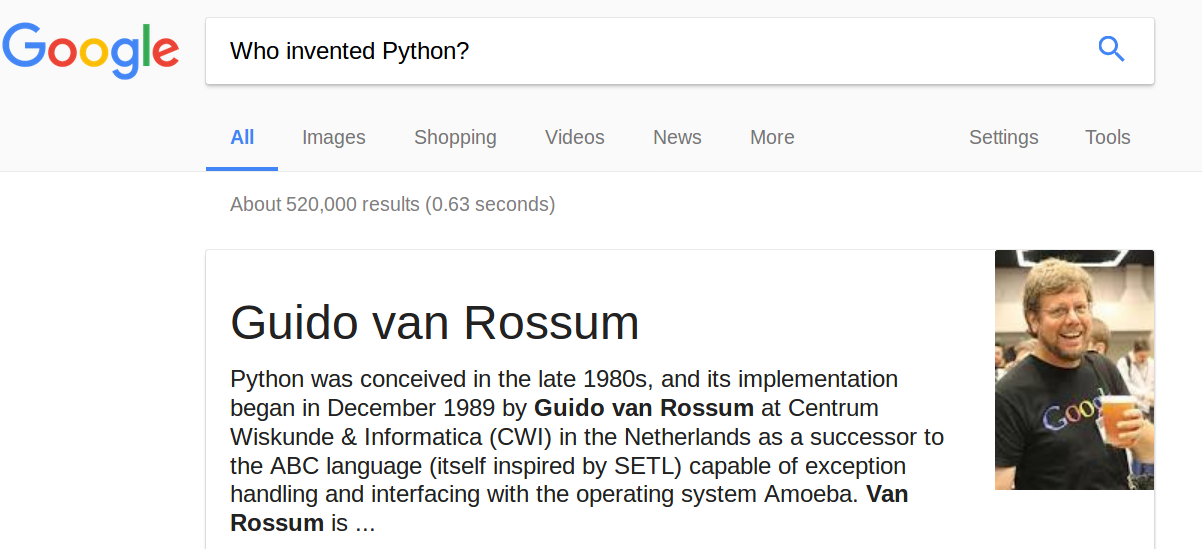
\includegraphics[width=1\linewidth]{./images/Chapitre1/guido_google.png}
	\caption{}
\end{subfigure}

	\begin{subfigure}[b]{0.55\textwidth}
	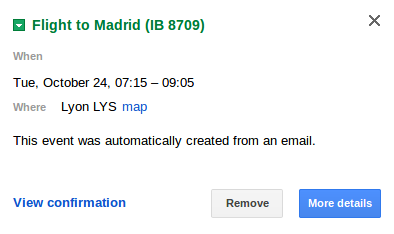
\includegraphics[width=1\linewidth]{./images/Chapitre1/calendar2.png}
	\caption{}
\end{subfigure}
\caption{(a) While searching \textit{Who invented Python?}, Google recognizes the simple question an directly gives us the answer from Wikipedia. (b) Gmail detects we received an email from an airline and parses it, finds the date, and automatically creates the corresponding event in our calendar.}	
\label{fig:google_nlp}
\end{figure}
%
Indeed, making computers learn,  via theories, algorithms and applications, is the general objective of artificial intelligence research \cite{Sugiyama2015}. Coming from this multi-disciplinary area, Natural Language Processing\footnote{And its more applied branch, text mining or text analysis. While it is sometimes argued that text mining deals with the structured data information extracted from text, I believe both terms considerably overlap nowadays. For ease of readability, in this dissertation we use both terms interchangeably, while preferring Natural Language Processing.} (NLP) is the domain that aims to make machines understand our language \cite{JurafskyM09} and thus making it possible to communicate with them in our own language. Specifically, speech and text, the latter being the focus of this work.

Although a challenging task, primarily given the ambiguity and dynamics of human language, NLP has developed rapidly \cite{ClarkBook2010} during the last two decades mainly due to the combination of three factors: 
\begin{itemize}
\item The  availability of \textbf{large quantities of freely-accessible textual data}: primarily enabled by the current Web technologies, we are today able to download with a single click the entire content of the English (or other languages) Wikipedia. In the same sense, we can also download thousands of gigabytes of Web crawled data. This information is used to derive knowledge about the text itself, as we will see in the rest of this dissertation. 
\item The \textbf{computational power} at our disposition: from consumer-based computers able to perform parallel computations with considerably large datasets; to on-demand distributed cloud platforms with high performance computing nodes. The latter may be from private providers, e.g., AWS Cloud Service\footnote{\url{https://aws.amazon.com/}}, Microsoft Azure\footnote{\url{https://azure.microsoft.com/en-us/}}, etc; or furnished by public organizations, such as France's Lyon 1 University\footnote{\url{https://p2chpd.univ-lyon1.fr/}} or the National Institute of Nuclear Physics computing centers\footnote{\url{https://cc.in2p3.fr/}}.

\item  The \textbf{large quantity of open-source text mining and data science analysis tools}. Luckily, it is becoming more common for NLP laboratories around the world to make their developments available to the general public, e.g, Stanford University CoreNLP\footnote{\url{https://stanfordnlp.github.io/CoreNLP/}}, Antwerp's University CLiPS Pattern\footnote{\url{http://www.clips.ua.ac.be/pattern}}.
% Paris 7's University Alpage Team Software\footnote{\url{https://www.rocq.inria.fr/alpage-wiki/tiki-index.php?page=Logiciels}}. 
Additionally, large Web companies, such as Facebook\footnote{\url{https://github.com/facebookresearch}} and Google\footnote{\url{https://github.com/google}}, frequently publish their research code and utilities. Lastly, communities of individuals develop libraries that grow to become essential building blocks of several applications and research in the domain. Notably, \texttt{scikit-learn}\footnote{\url{http://scikit-learn.org/}}, a popular data science library implementing several well-known machine learning algorithms. Regarding NLP specifically, two up-to-date libraries stand out:  \texttt{gensim}\footnote{\url{https://radimrehurek.com/gensim/}} and \texttt{spaCy}\footnote{\url{https://spacy.io/}}. These are, for the most part, cross-platform, high performance, optimized, well maintained, documented, and easily installable libraries.
% The former specializing on topic modeling and the latter on word's distributional representations.

\end{itemize} 
%
\begin{figure}
\centering
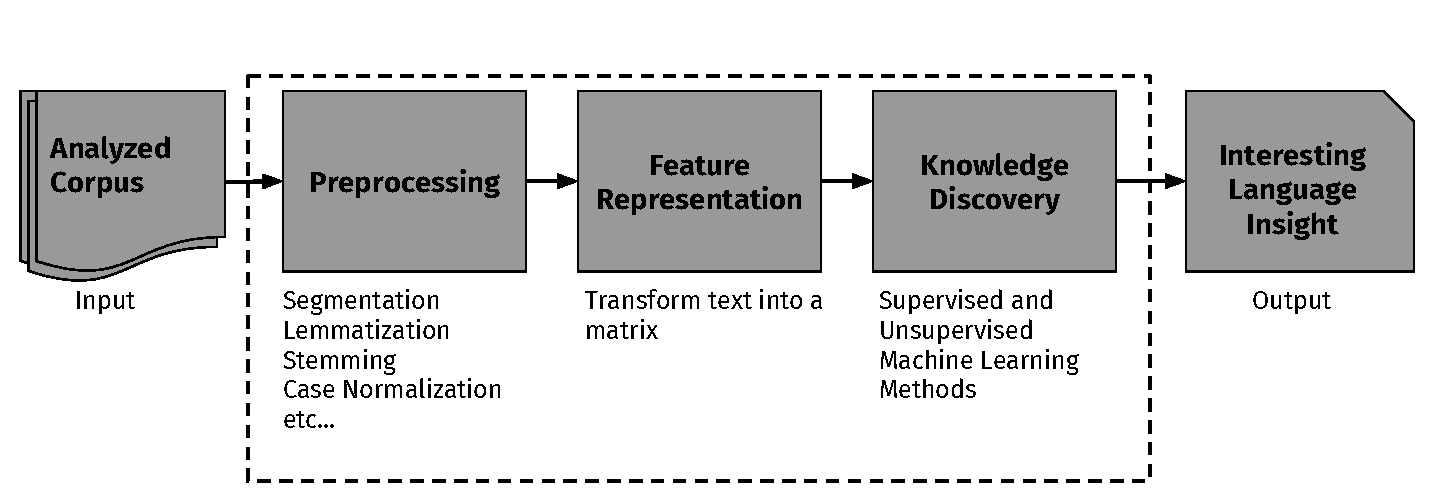
\includegraphics[width=1\linewidth]{./images/Chapitre1/nlp_flow.pdf}
\caption{Typical steps of Natural Language Processing applications.}
\label{fig:nlpflow}
\end{figure}
Solutions to NLP tasks generally follow three steps to achieve their respective goals \cite{mining12Book,JurafskyM09}. We can see in Figure \ref{fig:nlpflow}  the typical steps of a NLP system.  First, in \textbf{Preprocessing}, an input corpus is "normalized" so that it will be easier to treat it in the following steps. Secondly, in \textbf{Feature Representation}, numerous features are extracted from the preprocessed text. Thirdly, in \textbf{Knowledge Discovery},  a machine learning or rule-based (less common nowadays) technique is used to  learn a model able to provide an interesting insight within the existing data as well as on new future instances. The output of said system is usually the model or the language knowledge that reveals an interesting piece of information contained in the input corpus. 

Natural Language Processing is used today for several practical applications. From the elementary tasks that aim to extract linguistic features directly from the text, to more applied systems that employ said features to solve challenging problems. For example, as elementary tasks there is Part-of-Speech (PoS) tagging and Named Entity Recognition (NER). The former, PoS tagging, aims to determine a syntactic class (part of speech) for each word in a corpus \cite{JurafskyM09}. The latter, NER, determines if a proper noun is a place, a person, an organization or any other type of entity required by the final domain and application \cite{nadeau2007survey} . An intermediate task, Word Sense Induction and Disambiguation (WSI/WSD) determines and assigns the semantic meaning of a given word according to its context \cite{ClarkBook2010}.


More complex tasks that generally employ one or more of the aforementioned techniques in order to get more descriptive features from the text and thus get us closer to understand what is being discussed. As an example,  sentiment analysis which ultimate goal of this task is to determine the positiveness or negativeness (or neutrality) of an opinion expressed in a text \cite{liu2012survey}. In this case, it would be useful to know what words express a ``sentiment'': usually adjectives, categorized via PoS tagging; it would be informative to know what (or about who) we are talking about, with NER tagging; as well as the specific context of the words that are being used in the opinion, via WSI/WSD. 



\section{Challenges and Contributions}
There are several research challenges that arise from the choices taken in each one of the steps comprising the NLP system's flow (Figure \ref{fig:nlpflow}).
 In this thesis, we particularly focus on three challenges arising in both the Feature Representation and Knowledge Discovery phases. These challenges are: (1) modeling, extracting, and storing different types of linguistic features from raw text, (2) dealing with the sparsity inherent to text data features and also successfully combining them to get better representations, and (3)  finding	 relations  between words and then leveraging them in order to discover their latent relatedness and be able to solve NLP tasks.

%\begin{itemize}
% \item \textbf{Feature Representation:}
%	 \begin{enumerate}
%	 \item Modeling, extracting, and storing different types of linguistic features from raw text. 
%	 \item Dealing with the sparsity inherent to text data while successfully combining the different available text features.
%	
%	 \end{enumerate}
% \item \textbf{Knowledge Discovery:}
% 	\begin{enumerate}
% 	\item[3.] Finding relations  between words and then leveraging them in order to discover their latent relatedness and be able to solve NLP tasks.
%  	\end{enumerate}
%\end{itemize}


We propose three contributions, one in terms of theoretical modelization and two in terms of NLP applications. Specifically, the contributions that we propose in this work are the following:
\begin{itemize}
\item a hypergraph network-based model to hold and combine heterogeneous linguistic data %as well as a tool to extract said data from unstructured text.
\item a network-based algorithm to discover semantic relatedness between linked words
\item a method to combine heterogeneous representations while at the same time alleviating the sparsity problem common while dealing with text features.
\end{itemize}
These contributions are tested and evaluated using two different NLP semantic tasks: Word Sense Induction and Disambiguation, and Named Entity Recognition. We chose these two tasks as they are semantic problems directly benefited by those methods  that are able to determine the relatedness among words, which is the case of the techniques we propose. Not less important, we attack these tasks as they are central building blocks of more intricate text analysis systems. Our propositions are built using open source tools and trained/tested using freely accessible corpora. We aim to make our software implementations are  to multi-threaded CPU computers when applicable.


\subsection{Modeling linguistic features}
\paragraph{Challenge}
Representing unstructured text within a model that describes textual units and their corresponding features is a critical step within a NLP process. Textual units -- either words, sentences, paragraphs, documents, etc -- need to be represented by some kind of model that will allow for numerical analyses to be applied. Usually, textual units are represented in a vectorial space, where each dimension represents a feature; or in a graph-like structure, where features link units together. Concerning the features themselves, their selection is often an empirical process determined  by the final goal of the NLP process at hand. Nonetheless,  we have access to several types of linguistic features, each one representing the text from different points of view.  Furthermore, texts usually containing large vocabularies involves the need of an efficient way of storing a corpus and its features. These possibilities entail the following research questions: \textbf{what type of model can we employ to represent a corpus through a set of heterogeneous features, extracted from itself, while keeping record of the relationships between textual units?} \textbf{How can we organize and store this model as simply and efficiently possible?} Answering these questions would allow us to  properly design and build a linguistic resource containing heterogeneous descriptions of the textual units\footnote{In this work we focus on words. As such, the rest of this dissertation deals with the representation of words.} adapted to solve NLP tasks.


\paragraph{Contribution}
We propose a linguistic resource in the form of an heterogeneous language network to be used as a first essential data model to solve Natural Language Processing tasks. 
During the last decade, graphs have been used to model textual data given its ability to naturally represent the dynamics and structured of text.

The originality of our work consists in taking into account different types of features, e.g., lexical, syntactical, and orthographic information; and unifying them under a single hypergraph structure. An hypergraph differs from a graph in that its edges may link several nodes together at the same time. This flexibility allows for simple and efficient access to the stored elements, either specific types of words or specific features. (revoir: advantages of hyperedges]
%
We use the proposed model as the starting point of our other two contributions: solving Word Sense Disambiguation and Induction and Named Entity Recognition. 

Lastly, as a proof of concept and in order to test the implementation practicality of our model, we process the English Wikipedia corpus and store its heterogeneous features under the form of the proposed model. We particularly focus onto the lexical and syntactical characteristics of words.

\subsection{Leveraging the network to find semantic relatedness}
\paragraph{Challenge}
Leveraging the structure within the proposed linguistic network is one of our main reasons to build such a graph-based language resource. This structure, namely the features linking words  together, originate groups or communities of related words within the network. In that sense, leveraging these latent communities is still today an open question in the domain of graph-based NLP. Particularly in the context of semantic NLP tasks, where determining the relation among words is of utmost importance, we rise the following questions: \textbf{what kind of communities exist within language networks?} \textbf{How can we find and employ them to solve NLP tasks?} Furthermore, assuming an heterogeneous network like the one we propose, \textbf{what are the quantitative and qualitative differences, both in terms of performance and results, between the different representations existing within the network?} Determining the structure inside a language network, as well as devising an algorithm to exploit it would allow us to better understand the role of communities in  graph-based approaches for NLP. Finally, getting a glimpse of the differences between each heterogeneous feature can help us to decide which is the most appropriate according to a NLP system objective. 


\paragraph{Contribution}
Linguistic networks are complex structures that may hold  heterogeneous entities and links together. Properly leveraging these structures has been indeed a popular area of research in the NLP literature. 

We propose a variant to a literature algorithm that solves word sens induction and disambiguation mainly by leveraging  the structure of a language network in. The assumption of the algorithm is that of the network having "real-world" characteristics, broadly, this means that there are several tight-knit groups of words within the structure. Nonetheless, contrary to the existent model, our proposition differs regarding the considerably lower number of parameters by adjusting them automatically according to the statistics of the concerned network. We also allow for more flexibility of the studied contexts of each word. Furthermore, we leverage the structure of our proposed linguistic model and go beyond the classic homogeneous cooccurrences by studying the effect of heterogeneous features on the quality of the senses induced by the system. Our experiments show the interest of our method by improving on the performance of similar methods and by being on the same ballpark of state-of-the-art methods. We also thoroughly analyze the characteristics of the results --the word senses-- according to the different types of  obtained by our system.

 This We  improve the overall performance compared to other similar graph-based techniques.

\subsection{Combining features and dealing with sparsity}
\paragraph{Challenge}

While the proposed linguistic network contain heterogeneous features, in our previous propositions we have exclusively employed them separately. Nonetheless, employing these different attributes on a single textual representation is equally useful in terms of solving NLP applications. A certain type of feature may indicate relations that are completely unknown in another representation space. Thus a certain type of features can complement another to improve the overall description of words.

Another challenge that arises when building large cooccurrence networks, such as ours, is data sparsity. Indeed, sparsity is one of the main characteristics of textual data. Natural language processing systems rely on accurate information being found within a corpus. However, it is hard to see all the possible word cooccurrences in an input corpus and thus a system trained from it is not able to apply the acquired knowledge when it encounters unseen words and their cooccurrences.


Towards addressing both challenges previously described we pose the following questions: \textbf{how to alleviate data sparsity on textual data?}  Concerning combining linguistic features, h\textbf{ow can we produce a single textual representation  that is able to leverage the complementarity among features?} Lastly, \textbf{what is the behavior of combining features against using them independently?} The answer to these questions may shed light into more robust NLP systems, able to cope with sparsity while leveraging at the same time useful information coming from different types features.


% We explore multimedia fusion techniques to complement the features hold by the netuwork. Specifically, we focus on solving named entity recognition and word sense induction and disambiguation by applying feature-combination methods that have already shown their efficiency in the multimedia analysis domain.  Our results show that the combination of textual features indeed improves the performance compared to single feature representations and trivial features concatenation. Even more, we experiment with background information from open text sources to further improve the performance of our models. Finally, we also present an analysis on the behavior of features according to different types of senses and entity classes.



\paragraph{Contribution}
%\newpage












%\section{Contributions}
Addressing the sparsity of textual data is not an easy task and often involves complex procedures and loss of information. To alleviate this issue, we propose the application of multimedia analysis fusion techniques to solve NLP semantic tasks. The fusion methods we employ comprise a set of methods to combine (or fuse) different types of features into a single unique representation. While combining attributes we also enrich them by leveraging the complementary information  they carry individually. Furthermore, we address the challenge of data sparsity by transferring unseen relations from one feature space to another, that is, we obtain a denser similarity space by joining together both feature spaces. The experiments we carry out, in word sense induction and disambiguation and named entity recognition, show the pertinence of our approach. Specifically, we try different fusion techniques as well as several fusion configurations to improve the tasks' performance compared with using representations independently. Additionally, we study to what extent each type of fusion employed affects the performance of the tasks we evaluate.



\begin{figure*}
\centering
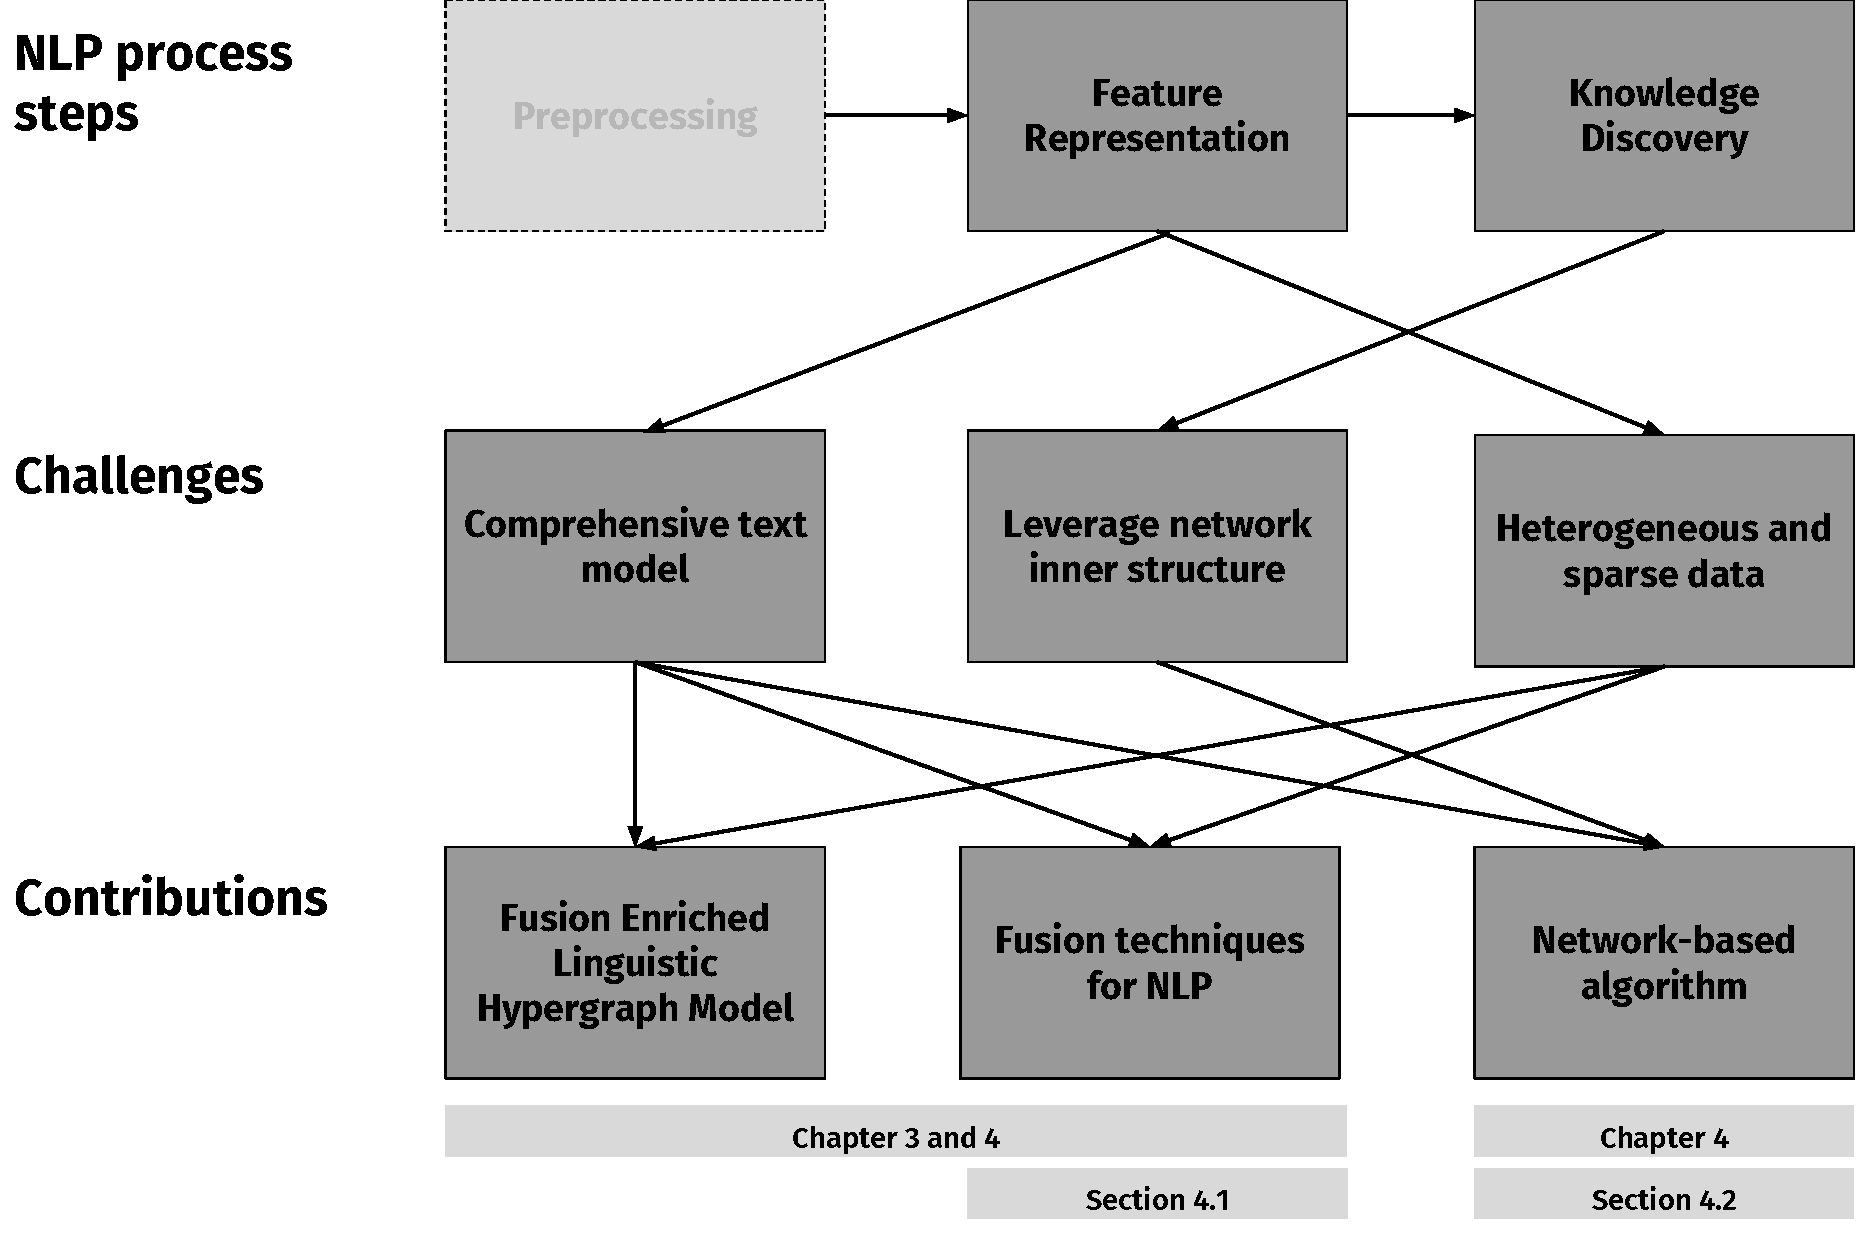
\includegraphics[width=1\linewidth]{./images/Chapitre1/challenges_contribs.pdf}
\caption{Block diagram of the NLP steps of interest, the challenges we address, and the contributions we propose.}
\label{fig:challenges_contribs}
\end{figure*}
\section{Structure of the Dissertation}

Figure \ref{fig:challenges_contribs} synthesizes the concerned NLP process-flow stages of this work (first line), the challenges that we aim to alleviate (second line), and their effect on the contributions we propose (third line). The remainder of this thesis is structured as follows. 

\paragraph{Chapter \ref{chap:backgnd}} This chapter contains the theoretical background on the concepts discussed in this thesis. At the same time, we present the state of the art on the techniques that are relevant to our work. Specifically, we discuss the basics on text representation and how they are all related together by the distributional hypothesis. We then introduce the two main types of mathematical entities to manipulate text in a computer: vector-space models and graph-based models. Given our choice to work with graphs, we continue this path and introduce the types of textual graphs that concern us. Finally, we describe an inherent problem to text data: sparsity.
%Afterwards, we present how these features can be combined to improve the results of single-feature based solutions. 
%Finally, we detail the machine learning methods we employ in certain as part of our methodology. 

\paragraph{Chapter \ref{chap:ling_net}} We begin by giving a review on how linguistic networks are used in the literature. This contextualizes our first contribution. We present and define a theoretical contribution: a novel structure to hold language information based on a hypergraph linguistic model.  We discuss its characteristics and the intuitions behind its conception: the choice of the structure,the role of nodes and heterogeneous edges, the type of features stored, the advantages it represents in terms of accessing and manipulating the data. Then, we introduce a set of techniques to make use of heterogeneous relations while dealing with sparsity, the feature fusion techniques. These methods are integral part of our contributions. Finally, we present a concrete application of our hypergraph model using the English Wikipedia. We describe its properties and motivations. The content of this chapter is drawn from \cite{sorianoJournal,sorianoLREC,sorianoEGCChallenge}.

%This chapter describes the process of parsing and storing an English Wikipedia Syntactical Dump. We use open source tools on freely available data to generate a software that is able to extract lexical and syntactic data from a given corpus.We thus create and publicly release a syntactically annotated version of the English Wikipedia containing often-neglected information, stored in a format that facilitates its manipulation. 
\paragraph{Chapter \ref{chap:wsd}} In this chapter, we present our two applied contributions. First, an algorithm that exploits the structure of the network, i.e., the connections between nodes to solve word sense induction and disambiguation. 
%Namely, we derive senses from a test corpus by finding related words connected to a single main node.
We test the linguistic and lexical features and discuss about its qualities. Our results improve on the performance of similar propositions from the literature.
% We study the combination of features using multimedia fusion techniques in the next chapter.
Secondly, we explore the application of multimedia fusion techniques using linguistic features to solve NLP tasks. 
%Briefly, fusion techniques may consist on trivially concatenating feature columns or a combination that aims to transfer relatedness information from one representation to a second one. 
We experiment with these methods on three datasets for named entity recognition and one dataset for word sense induction and disambiguation. Indeed, we show that using certain configurations of fusion techniques can lead to improvements over single-feature and trivial-concatenation representation matrices. Furthermore, we explore the contribution from each feature space for each sense and class in each task respectively. This work has been published or accepted for publication in \cite{sorianoCICLING,sorianoDS}.	

\paragraph{Chapter \ref{chap:conclusions}} We conclude this dissertation and present possible avenues for future work.


\chapter{Background}
\label{chap:backgnd}
\begin{abstractchap}
This chapter goes into detail about the notions of the theoretical our work is based on. First, we introduce the distributional hypothesis and the parameters involved in the generation of descriptive contexts from a corpus. Secondly, we present how can we describe the distributional contexts within a model, either directly through a vectorial representation or by means of a graph-based representation. Thirdly, we discuss one of the main challenges of dealing with textual data: data sparsity. We cover what is it, its consequences, as well as existent solutions to it. Finally, we summarize the concepts introduced and contextualize our propositions.
\end{abstractchap}
\minitoc

\section{Distributional Hypothesis}\label{sec:disto_hyp}
The work we present in this thesis is prominently based on the distributional hypothesis (DH). This is also the case for the large majority of semantic approaches in NLP today. This context-analysis insight is usually credited primarily to \cite{harris1954}. The hypothesis is simple yet powerful: it can be formulated as "You shall know a word by the company it keeps." \cite{firth57synopsis}. More formally, it states that the similarity of meaning correlates with the similarity of the word's context distribution. It follows that the meaning of a word can be determined by the set of contexts in which it occurs in a corpus. Consequently, for two target words, the larger the number of shared contexts, the semantically closer these words are. 

\begin{figure}
\centering
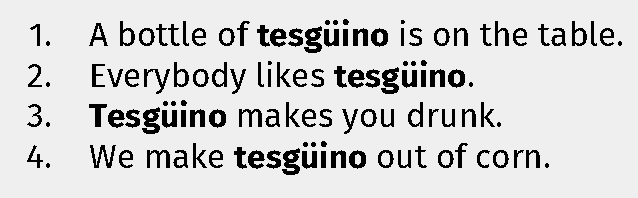
\includegraphics[width=.6\linewidth]{images/Chapitre2/tejuino.pdf}
\caption{Even though \textit{tesg\"{u}ino} is a relatively obscure word, from its context we can understand its an alcoholic drink made from corn.}
\label{fig:tejuino}
\end{figure}


Taking the classic example by \cite{nida1979componential}, shown in the four lines  in Figure \ref{fig:tejuino}, even if we do not know that the word tesg\"{u}ino (or tejuino) rinedefers to a ceremonial corn beer consumed by the native people of the north of Mexico, we can infer, by looking at its context, that we are indeed referring to some sort of corn alcoholic beverage. We can then easily infer that tesg\"{u}ino is similar to other drinks such as tequila or mezcal.



Although we usually find in the literature that the work of Harris is the most important concerning the DH, we should note that the hypothesis rests on two theories  \cite{sahlgren2008distributional,turney2010}: the statistical semantics hypothesis \cite{booth1955machine}, and the  structuralism theory, as described by \cite{de1916course}. The former is important as it places the DH within a larger context. Broadly, it affirms that statistical patterns of human word usage can be employed to understand what people mean. The latter,  gives the DH a more robust approach towards the definition of what kind of distributional context  we should use to determine similarities, as well as what does the meaning of the contextual relations between words implies. In plain words Saussure's version of the structuralist theory indicates that the differences in the contexts of a word determine its role within a language system. 

To this end, Saussure proposed two kinds of context relations: syntagmatic and paradigmatic. Syntagmatic relations concern the context defined by words that co-occur in the text, such as collocations (multi-word expressions that occur frequently in a corpus) and colligations (relations between a lexical item and a grammatical category) \cite{verschueren2015handbook}. On the other hand, paradigmatic relations associate words according to whether they appear or not in the same context. Put differently, these are words that tend to not appear together while sharing the same context. These type of relations define classic semantic relations such as synonymy-antonymy or hypernymy-hiponymy. Coupling both the DH with structuralist theory gives birth to the more fine-grained definition of the distributional hypothesis, introduced by \cite{sahlgren2008distributional}: the refined distributional hypothesis. We note that this distinction, syntagmatic versus paradigmatic relations, is also more recently defined in \cite{schutze1993vector}. In their work, syntagmatic relations are called first-order co-occurrences, while paradigmatic relations  are referred to as second-order co-occurrences.

\begin{figure}
\centering
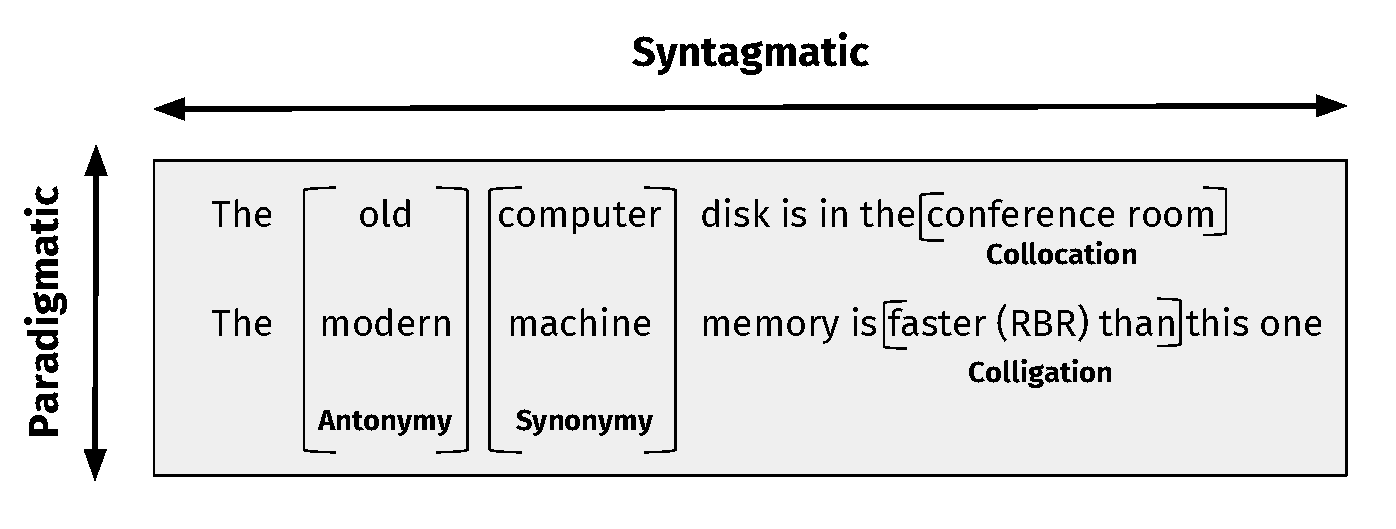
\includegraphics[width=\linewidth]{images/Chapitre2/sintagmatic_paradigmatic.pdf}
\caption{Examples of syntagmatic and paradigmatic contexts and their corresponding semantic relationships. Based on the examples by \cite{sahlgren2008distributional,piero2017}.}
\label{fig:sintagmatic_paradigmatic}
\end{figure}


An example of syntagmatic and paradigmatic relationships can be seen in Figure \ref{fig:sintagmatic_paradigmatic}. Vertically looking at the words \textit{old} and \textit{modern} (in the first and second phrase respectively), we can say that they  share a paradigmatic context, as they tend to not occur together, either we write old \textit{or} modern, while sharing the same context (either \textit{computer} or \textit{machine}). In this case, that leads to an antonym semantic relation. Something similar happens with the words \textit{computer} and \textit{machine}, this time sharing a synonym relation. With respect to the syntagmatic relationships, horizontally looking at the words, we find the collocation \textit{conference room} in the first phrase, as well as the colligation in the second expression between the word \textit{than} usually preceded by a  comparative adverb (RBR), which is \textit{faster} in this case. 

In spite of Sahlgren's  distributional hypothesis definition, determining the types and meaning of semantic relations, obtained with distributional methods, is still an open challenge on distributional models and methods. Determining the specific type of semantic relation (e.g., synonymy, hyponymy, meronymy) is still an open issue in the community \cite{turney2010,fabre2015,perinet2015}. While distributional models can give us fast access  to semantic relations between words within a corpus, they are most of the times ambiguous relations. It is still our task, as users, to determine the type of semantic relations found, in the case these distinctions are needed by the NLP system  at hand.
% We note that our work does not delves into the study of the semantic relations but we use them to relate 

Distributional methods, based on the DH, have been used for a long time now \cite{JurafskyM09}, although computationally automatized since the 1990s \cite{perinet2015}. Being a mature research field, systems based on these distributional models are varied and cover a large range of NLP tasks being obviously most popular on semantic tasks \cite{bruni2014multimodal}. We do note that nowadays, they have somewhat resurfaced (although they really never went away) thanks to the recent re-introduction of word embeddings, or simply word distributional representations. In short, a word embedding, in the context of newer developments, is a vectorial representation  that "embeds" words into a low-dimensional space, usually generated either by means of some sort of matrix reduction \cite{lebret2013deep,levy2014neural} or by using neural networks \cite{Collobert2011,mikolov2013distributed}. These representations are usually obtained from very large bodies of text and they have shown to be quite effective for solving NLP tasks.

The actual implementation of a distributional model consists in three steps: (1) determine what type of context is going to be used, (2) chose a computable context representation, and (3) determine a weighting scheme  and a  relatedness measure.

%\subsection{Types of Context}\label{sec:contexts}
We move now onto the description of what are the types of contexts commonly used while implementing a distributional model to represent words.  We cover two types: lexical co-occurrence and syntactic co-occurrence. In this work we will exclusively focus on those two contexts. The first one describes a word's context based on its nearby words.  The second defines a word's context according to the syntactic relations between the word and its neighbors. We will use the example phrases in Figure \ref{fig:example_phrases} to illustrate the kind of contexts we will describe below. 
\begin{figure}
\centering
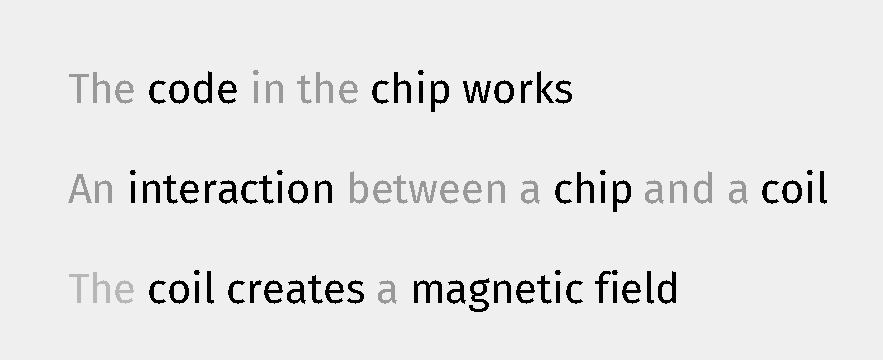
\includegraphics[width=0.7\linewidth]{images/Chapitre2/example_phrases.pdf}
\caption{Example text. Functional words are grayed-out. }
\label{fig:example_phrases}
\end{figure}

%todo Add as footnote the distinction between similarity and relatedness in Turney, Jurafsky, et al
%todo Define what is a target word (first time i talk about target word??)
%todo Add that a "Topical semantic relatedness" is obtained when context window is larger


\subsection{Lexical Contexts}
Also called linear contexts, lexical contexts consist on those  words that co-occur with a given word in a predetermined neighborhood: either in a sentence, a paragraph or larger units of text such as full documents \cite{LevyG14,sahlgren2008distributional}. Nowadays, the lexical context is usually determined by a window of $n$ tokens to each side of the target word. As an example is shown in Table \ref{tab:exo_lexical_contxt}, where the context -2+2 of the words \textit{code}, \textit{chip}, and \textit{coil} is shown. The size of the context depends of course of the application of the system. Indeed, determining the size  is actually a quite empirical decision. Nonetheless, it seems that today the literature \cite{Daume2006,mikolov2013distributed,LevyG14,levy2014neural}  has settled for a two-words to the left and two-words to the right context window (plus the target word), otherwise represented as -2+2. \cite{sahlgren2006word} discusses  the motivations of selecting a window of a particular size. He notes that given the literature evidence,  a shorter context window (specifically a -2+2 window) is preferable for acquiring semantic information. In this sense, \cite{JurafskyM09} determines that generally the context size used lies between 1 and 8 words on each side, or 3 and 17 in total. In practical terms, the choice of the size  affects the scope of the semantic relatedness: the shorter the context, the more specific is the information about a target word, approaching syntactic relations. Furthermore, these relations are "stronger" in the sense of being semantically similar, we could in theory substitute one word for another as the shared relation is synonymy. On the contrary, the larger the window, the broader the information conferred by the context words. 



% Please add the following required packages to your document preamble:
% \usepackage{booktabs}
\begin{table}[]
\centering
\caption{Lexical contexts of the words \textit{code}, \textit{chip}, and \textit{coil} appearing in each one of the phrases on Figure \ref{fig:example_phrases}. The context is paradigmatic, the window being the word and 2 words to the left and right.}
\label{tab:exo_lexical_contxt}
\begin{tabular}{@{}ll@{}}
\toprule
Words & Lexical Context                        \\ \midrule
code  & code;\textbf{w+1}:chip; \textbf{w+2}:works                    \\
chip  & \textbf{w-2}:interaction; chip; \textbf{w+1}:coil \\
coil  & coil;\textbf{w+1}:creates; \textbf{w+2}:magnetic              \\ \bottomrule
\end{tabular}
\end{table}

Lexical co-occurrences are the most popular way to represent distributional contexts. They are easy to obtain as there is no need for external information except the input corpus itself. 
 




%\subsection{Lexical Representations}
%\subsection{Syntactic Representations}
%
\subsection{Syntactic Contexts}

The second type of context depends on a more profound analysis of text. As its name implies, syntactic contexts are based on the analysis (or parsing) of text in order to obtain sense from them. Lexical contexts are able to somehow take into account the order of appearance of words in a phrase. Still, words in a sentence are not related among them like a list: semantic information is indeed extracted from words themselves, however syntax highly affects the way information is combined into semantic structures. Words tend to form groups between themselves, called constituents or chunks, which relate to other constituents to form a single phrase unit \cite{bender2013linguistic}.

\paragraph{Constituent Tree}
Indeed, constituents are  represented with tree structures aptly named  constituents parse tree, or simply parse tree (see Figure \ref{fig:exo1_constits}) \cite{JurafskyM09}. These trees actually represent the context-free grammars models that we use to describe the chunk structure. As such, the parse tree differentiates between terminal, pre-terminals and non-terminal nodes. Non-terminal nodes refer to chunk labels (e.g., noun phrases\footnote{The nomenclature used is the Penn Tree Bank annotation.}: \textit{NP}, verbal phrases: \textit{VP}, prepositional phrases: \textit{PP}), pre-terminal nodes pertain to Part of Speech (PoS) categories (e.g., determinants: \textit{DT}; adjectives: \textit{JJ}; nouns: \textit{NN}). Finally, terminal nodes indicate the word itself. 

%todo References, who is using constituents trees??
A constituents tree is illustrated in Figure \ref{fig:exo1_constits}. The image corresponds to the parse tree of the first phrase of the example in \ref{fig:example_phrases}: \textit{The code in the chip works}. From the bottom-up,  looking at the node labeled \textit{chip}, we see it is a token of type noun (pre-terminal labeled \textit{NN}) and it belongs to a noun phrase (non-terminal \textit{NP}) which in turn belongs to a prepositional phrase (\textit{PP}) which finally is part of the main noun phrase of the sentence \textit{S}. Constituents usually include a word with a prominent role: the \textbf{head} of the constituent. In practical terms, the head (or governor) is the most important word in the chunk because it determines what kind of words (either a verb, an adjective, a noun, etc.) will be joining it within the constituent. 

The context that can be extracted from a constituency parse is similar to that of the lexical contexts, in that words themselves are part of the co-occurrent neighborhood. Yet, with the information from the parse tree, we can restrict the window to a chunk and heal consider only certain structural units. The context of \textit{code} and \textit{chip} of the parse  in Figure \ref{fig:exo1_constits} are shown in Table \ref{tab:exo_constits_contxt}. They consist simply in the non-functional words that co-occur with each word in a given constituent, in this case a noun phrase (NP).

\begin{figure}[t!]
	\begin{minipage}{\textwidth}
		\begin{minipage}{.9\textwidth}
			\centering
			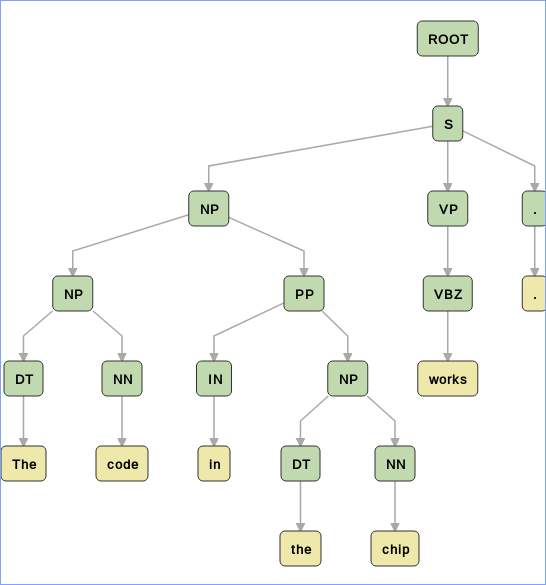
\includegraphics[width=0.7\linewidth]{images/Chapitre2/exo1_constits.png}
			\captionof{figure}{Constituents tree parse of the phrase \textit{The code in the chip works.}}
			\label{fig:exo1_constits}
		\end{minipage}
		\\
		\\
		\begin{minipage}{.9\textwidth}
			\centering
			\begin{tabular}{@{}ll@{}}
			\toprule
			Words & Syntactic Context                        \\ \midrule
			code  & \textbf{NP}:chip                    \\
			chip  & \textbf{NP}:code \\
			\end{tabular}
			\captionof{table}{Syntactic contexts, based on the constituents tree in Figure \ref{fig:exo1_constits}, corresponding to the words \textit{code} and \textit{chip}, from the first phrase on Figure \ref{fig:example_phrases}.} 
			\label{tab:exo_constits_contxt}
		\end{minipage}
	\end{minipage}
\end{figure}

%TODO What is a grammar?
\paragraph{Dependency Tree}
While  a parse tree represent the units existing within a specific group of syntactically related words, as a complementary approach, we can also formalize syntactic information with dependency trees. This time, the syntactic structure of a sentence is described in terms of words and asymmetric binary grammatical functions between these words   \cite{ClarkBook2010}. The trees are directed, all nodes are terminal and they represent words and they are linked following a direction from the head to its \textbf{modifier} (or dependent). An edge thus represent one of these dependency functions which are labeled  with tags that, just as PoS tags and chunk tags, describe what kind of relation exists between two words \cite{bird2006nltk}. For example, the Universal Dependencies\footnote{This set of tags share a large quantity of labels with the more classic Stanford Dependencies \cite{de2006generating,de2008stanford} tagset. Briefly, universal dependencies aim to develop cross-linguistically and cross-language consistent annotations  \cite{nivre2016universal}.} tagset \cite{nivre2016universal,schuster2016enhanced}, which we use in this work, includes tags such as  \textit{det}: determiner, the relation between a noun head (governor) and its determiner, \textit{nmod}: nominal modifier, the same but with a modifier, or \textit{conj}: conjunction, two elements connected by a conjunction.

To illustrate dependency trees, we can observe in Figure \ref{fig:exo1_dependences} the dependency parse of the second phrase shown in \ref{fig:example_phrases}. In this particular case, the relation tags used are the "enhanced" universal dependencies by \cite{schuster2016enhanced}. The difference is that relations are made more explicit by collapsing them (reducing two relation edges into a single one)  and including the modifier  (or adjunct) directly into the label. Consequently, they can be more useful to determine the relatedness between words.

The context that can be extracted from dependency relations varies. Still, the usual consensus is to treat the relation as the triple it is: $(head, relation, dependent)$ and based on it extract a certain type of context. In the example of Figure \ref{fig:exo1_dependences}, a context of the word  \textit{chip}, according to \cite{Lin1997} would be: $(conj:and,coil,head)$. This indicates that \textit{chip} is connected to \textit{coil} by the conjunction \textit{and}. More recent context definitions, such as those of \cite{baroni2010distributional,LevyG14,Panchenko2017} also include the inverse relation a word participates in, i.e., if the target word is a dependent, its dependency relation is also included but indicated as "inverse".  Again, using the previous example with the  word \textit{chip}, the  contexts now would then be: interaction/nmod:between$^{-1}$; coil/conj:and . These contexts and other example can be seen in Table \ref{tab:exo_deps_contxt}.

\begin{figure}[!t]
 \begin{minipage}{\textwidth}
  \begin{minipage}{.9\textwidth}
    \centering
	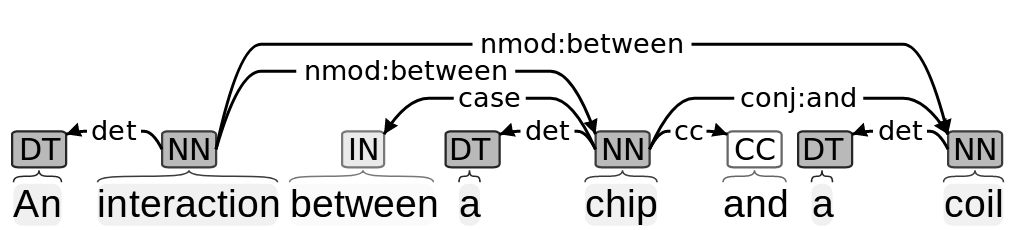
\includegraphics[width=0.9\linewidth]{images/Chapitre2/exo1_dependences.png}
    \captionof{figure}{Dependency tree parse of the phrase \textit{An interaction between a chip and a coil.}}
    \label{fig:exo1_dependences}
  \end{minipage}
  \\ 
  \\
  \begin{minipage}{.9\textwidth}
    \centering
		\begin{tabular}{@{}ll@{}}
		\toprule
		Words & Syntactic Context                        \\ \midrule
		interaction  &   coil/nmod:between; chip/nmod:between                   \\
		chip  & interaction/nmod:between$^{-1}$; coil/conj:and \\
		coil  & interaction/nmod:between$^{-1}$; chip/conj:and$^{-1}$      \\ \bottomrule
		\end{tabular}
		\captionof{table}{Syntactic contexts, based on the dependencies tree in Figure \ref{fig:exo1_dependences}, corresponding to the words \textit{interaction}, \textit{code}, and \textit{chip}, from the second phrase on Figure \ref{fig:example_phrases}} 
		\label{tab:exo_deps_contxt}
    \end{minipage}
  \end{minipage}
\end{figure}

Syntactic contexts are less used than their lexical counterpart in large part due to the process of obtaining the trees discussed before. While nowadays there are several software solutions able to extract this kind of information, the process is decidedly more complex than counting words in a lexical context setting. Furthermore, the information is not 100 \% accurate, as the systems are trained using human annotated banks of trees (called treebanks) which is in itself an ambiguous and hard process \cite{JurafskyM09,perinet2015}.  This difficulty stems yet another problem with syntactic information: syntactic parsers are not easily available for languages other than English and the rest of those in  the indo-european family. As a last downside, these contexts are known to generate sparse computational representations as they are more specific than simpler lexical contexts \cite{sahlgren2006word}. Still, syntactic contexts are shown to be able to contribute more information about word's relations than simple lexical contexts \cite{Lin1997,pado2003constructing,turney2010,baroni2010distributional,LevyG14,Panchenko2017}. In other instances, lexical contexts are shown to perform better in NLP tasks except when the syntactic contexts are extracted from very large corpora (such as Google Syntactic N-gram corpus \cite{goldberg2013dataset} containing $10^{11}$ tokens) \cite{kiela2014systematic}.

We have presented the two  main types of co-occurrence contexts that can represent a word in a corpus. In the next section we present the structures that allow mathematical and computational manipulation of the information provided by these contexts.







%\blindtext %1 %7 lineas x 8.3 =~ 60 lineas


\section{Vector Space Models}

The whole point of determining contexts, either lexical or syntactic, for a set of words in a corpus is to be able to assess how similar their meaning is among them. This assessment of relatedness thus need to be measured by a metric in order to determine its level. The way we measure the relatedness between words relies on well-known algebraic operations, such as the dot  product. In order to calculate a dot product we need vectors. It follows that to calculate relatedness among words we need to represent words by means of vectors, where each vector describe a word and each dimension a context of it. 

The Vector Space Model (VSM) consists in representing textual units in a multi-dimensional space. The textual units represented are not constrained to words themselves. We may describe co-occurrent features for documents, phrases, paragraphs, or other types \cite{manning1999foundations}. A matrix is used as the structure that holds each object and its context features. Indeed, in practical terms, a VSM is then an array of real-number vectors, where each one represent a text unit and the columns describes the co-occurrent contexts the word participates in. To illustrate  this, in Table \ref{tab:lexical_matrix} we represent words of the previous examples in a \textit{word space}. Each entry of this matrix (called a co-occurrence matrix) represent a weight that infers the importance of the row word (or target word) with respect to the column (context) co-occurrence in a given context, within an input corpus \cite{JurafskyM09}. That is, the word \textit{code}, co-occurs once with the context indicated by the second and third columns, which in turn correspond to the words \textit{chip} and \textit{works}.
%We note that some vector space models are not constrained to 2-dimensional matrices and leverage structures of larger dimensions \cite{baroni2010distributional}.

In the example, the weights consist merely on the frequency of co-occurrence of each word with each context. Indeed, there are still other two related parameters that affect the meaning extracted from a distributional model: the weight each cell in the matrix has, or how do each co-occurrence affect each word; and the similarity measure  between vectors we will use to determine the semantic relatedness among words. For a complete analysis on a wide range of parameters affecting vector space models, see \cite{baroni2010distributional,kiela2014systematic,levy2015improving}.



\begin{table}[]
\centering
\caption{Matrix representation of the lexical contexts of the words appearing in the phrases of Figure \ref{fig:example_phrases}. The window is the complete phrase where the word occurs.}
\label{tab:lexical_matrix}
\begin{tabular}{@{}lrrrrrrrr@{}}
\toprule
 Words & \multicolumn{8}{c}{Contexts} \\ \midrule
       & $w_1$ & $w_2$ & $w_3$ & $w_4$ & $w_5$ & $w_6$ & $w_7$ & $w_8$ \\ \midrule
code$_{w_1}$        & 0    & 1    & 1     & 0           & 0    & 0       & 0        & 0     \\
chip$_{w_2}$        & 1    & 0    & 1     & 1           & 1    & 0       & 0        & 0     \\
works$_{w_3}$       & 1    & 1    & 0     & 0           & 0    & 0       & 0        & 0     \\
interaction$_{w_4}$ & 0    & 1    & 0     & 0           & 1    & 0       & 0        & 0     \\
coil$_{w_5}$        & 0    & 1    & 0     & 1           & 0    & 1       & 1        & 1     \\
creates$_{w_6}$     & 0    & 0    & 0     & 0           & 1    & 1       & 1        & 1     \\
magnetic$_{w_7}$    & 0    & 0    & 0     & 0           & 1    & 1       & 0        & 1     \\
field$_{w_8}$       & 0    & 0    & 0     & 0           & 1    & 1       & 1        & 0     \\ \bottomrule
\end{tabular}
\end{table}

%todo slides the word-embeddings.pdf page 34 would be cool to put in this chap
%1 weighting
\subsection{Matrix Weights}

The weight is an important parameter in the creation of a VSM for a NLP application. Weights can be binary, simply  indicating presence or absence. They can count the number of co-occurrences of a word and the context, their absolute frequency. Weights may also be a type of discriminative measure that usually tries to give more importance to those contexts that co-occur more frequently with the target word while being less frequent  with the rest of the words in the text \cite{JurafskyM09,ClarkBook2010}.  

Point-wise Mutual Information (PMI) \cite{Church1990} and Positive Point-wise Mutual Information (PPMI) \cite{niwa1994co} are two popular choices to weight terms in a co-occurrence matrix \cite{turney2010,JurafskyM17}. We describe both of them below.

Given a co-occurrence matrix M, containing $W$ words (rows) and $C$ contexts (columns), where $f_{ij} \in \mathbb{R}^{W\times C}$ denotes the frequency of  target word $w_i$ frequency in the context $c_j$ , i.e., how many times they both co-occur. $N=\sum_{i=1}^W\sum_{j=1}^Cf_{ij}$ represents the sum of all the matrix cells. PMI is defined as:
\begin{equation} \label{eq:pmi}
PMI(w_i,c_j) = \log\dfrac{P(t_{ij}|c_j)}{P(t_{ij})P(c_j)}
\end{equation}
where  $P(t_{ij}|c_j)=\dfrac{f_{ij}}{N}$ tells us how many times the word and the context appeared together, normalized by the total context frequency. $P(t_{ij})= \dfrac{f_{ij}}{N}$, and $P(c_j)=\dfrac{f_j}{N}$. The ratio gives us an estimate of how much more the target and context co-occur than we expect by chance.

While PMI is often used as a weighting choice, it has three main downsides \cite{JurafskyM17,levy2015improving}: (1) PMI is biased towards co-occurrences of rare events, that is, a low-frequency context $c$ co-occurring with any word $w$ will yield a large PMI. Also (2), PMI may yield negative values, which would indicate a certain level of semantic "unrelatedness", which is not a  very intuitive concept. And (3),  if a context and a target word are not observed together (something that is very possible to happen because the co-occurrence matrix is sparse, we will look into that in the following paragraphs), the denominator of \ref{eq:pmi} is zero and thus $PMI_{ij}$ becomes undefined. 

To solve the first issue, \cite{levy2015improving} proposes a smoothed version of PMI, defined as:
\begin{equation} \label{eq:pmi_levy}
PMI_\alpha(w_i,c_j) = \log\dfrac{P(t_{ij}|c_j)}{P(t_{ij})P_\alpha(c_j)}
\end{equation}

with $P_\alpha(c_j) = \dfrac{f_j^\alpha}{N^\alpha}$, where $\alpha$ is a smoothing parameter that affects the contexts counts in order to alleviate the bias of PMI towards rare contexts co-occurrences : the probability of a low-frequency context $c_j$ will be larger thanks to $\alpha$, which makes the denominator of \ref{eq:pmi_levy} larger, which in turns make PMI$_\alpha$ smaller. Thus, addressing the bias for all words when co-occurring with a low-frequency context.


The second and third inconvenient are resolved by using Positive Point-wise Mutual Information (PPMI). PPMI simply replaces all values lower than zero (including $-\infty$) by a zero:
\begin{equation} \label{eq:ppmi}
PMI(w_i,c_j) = \max(PMI(w_i,c_j), 0)
\end{equation}
%2 similarity
\subsection{Defining Vector Similarity}
%3 sparsity (long, important paragraph)
The second parameter to consider after weighting the co-occurrence matrix is how to actually determine the similarity between two word vectors.

As with weighting schemes, there are multiple metrics (defined and compared to greater detail in \cite{ClarkBook2010,ferret2010testing,kiela2014systematic,clark2015vector}) used in the literature to determine the similarity between two vectors. We will focus on two that are of interest to this thesis: cosine and Jaccard similarity. More types of metrics and their comparison can be found in the previously cited literature. While there does not seem to be a single best measure of similarity, we usually use the cosine similarity, as it naturally can deal with real-valued vectors. On the other hand, when dealing with binary presence-absence vectors, it is more common to use Jaccard similarity. 

\subparagraph{Cosine Similarity}
The cosine similarity determines the angle between two multidimensional vectors. It is simply defined as the dot product between two vectors, normalized by the multiplication of their Euclidean length \cite{Manning2008}. The cosine similarity is bounded between $[0,1]$, yet we usually interpret the result in the positive space, where 0 means there is an angle of $90^\circ$ between the two word vectors, thus  no similarity at all; and 1 means there is no angle between them, so they are completely similar. Furthermore, if the weights of the matrix are non-negative values, the cosine similarity is bounded to the range $[0,1]$. The cosine similarity is defined as:
\begin{equation}
sim_{cosine}(\overrightarrow{w_1},\overrightarrow{w_2})  =  \dfrac{\overrightarrow{w_1}  \cdot \overrightarrow{w_2}}{||\overrightarrow{w_1}||\,||\overrightarrow{w_2}||} = \dfrac{\sum_{i=1}^Cw_{1_i}\times w_{2_i} }{\sqrt{\sum^C_{i=1}w_{1_i}^2}\sqrt{\sum^C_{i=1}w_{2_i}^2}}
\end{equation}

\subparagraph{Jaccard Index}
Also known as the Tanimoto index, the Jaccard index \cite{jaccard1908nouvelles} determines the similarity between binary vectors, it is defined, in terms of dot products:

\begin{equation}
sim_{Jaccard}(\overrightarrow{w_1},\overrightarrow{w_2}) = \dfrac{\overrightarrow{w_1} \cdot \overrightarrow{w_2}}{||\overrightarrow{w_1}||^2+||\overrightarrow{w_2}||^2 - \overrightarrow{w_1}\cdot\overrightarrow{w_2}}
\vspace{1cm}
\end{equation}

In terms of two sets, $A$ and $B$, the Jaccard index  calculates the ratio between the cardinality of the intersection of two word vectors divided by the cardinality of their union: $sim_{	Jaccard}(A,B)=\dfrac{|A \cap B|}{|A \cup B|}$. We prefer the definition in terms of dot products because in that way it is more straight-forward to implement it computationally.

We have been discussing vectorial space representations and their parameters (matrix weighting, similarity measure). While VSM models are the most popular to describe the semantic similarity between words, there are other structures that make it easier to  model the interactions that take place among lexical units within a corpus. In that sense, in the next section we introduce the fundamentals of graph-based representations for NLP, which are part of the contributions of this thesis.


\section{Network Models}
Network\footnote{We will use the notion of \textit{network} and \textit{graph} interchangeably during the rest of this dissertation, unless stated otherwise.} based models have been studied deeply during the last years in the NLP field  \cite{Mihalcea2011}. While we can represent a graph as a matrix, and thus as a vector space model, graphs are useful representation formalism that can be applied to a large set of linguistic characteristics, from the relation between words in a text or between the features that describe them. Indeed, language being a dynamic complex system, networks provide an adequate model to represent and study the structure and evolution of linguistic systems \cite{Choudhury2009}. 

Furthermore, based on graph theory, we can conceive efficient and sophisticated solutions to NLP tasks, such as PoS tagging, role-labeling, word sense induction and disambiguation, chunk parsing \cite{Mihalcea2011}. Notably, NLP graph-based approaches are largely employed to solve unsupervised tasks, where we can expect to get insights from the data by looking at  the links existing between entities; and semi-supervised problems, again by leveraging relations to propagate across the network small quantities of hand-crafted tags \cite{nastase2015}. An additional non-negligible advantage of graph models are that they allow human interpretation and analysis through their visualization (nonetheless with relatively small samples of text). 


Based on the  advantages just mentioned, in this thesis we base our linguistic\footnote{We will refer to a linguistic representation as an structure that holds textual units linked by their linguistic features, in this case, distributional co-occurrences.} model proposition on a graph-based structure. In the following paragraphs we discuss the types of networks used to represent textual data, which closely relates to the co-occurrence representations that we covered in the vector space model. Indeed, graph-based methods follow the same distributional principles as VSM. Thus, as we will see, the relationships among nodes on these networks are very similar to the types of contexts described in Section \ref{sec:disto_hyp}.


\subsection{Linguistic Networks}
A graph is a data structure consisting of a set of vertices connected by
a set of edges that  model relationships between objects.
Formally it is defined as a set $G=(V,E)$, where $V$ is a
collection of vertices $V=\{V_i,i=1,n\}$ and $E$ is a collection of
edges over $V$, $E_{ij}=\{(V_i,V_j),V_i \in V, V_j \in V\}$. 

When referring to language networks, nodes represent lexical units (most of the time words) and the edges represent the relationships between words. We present below the types of linguistic networks. 

\subsection{Types of Linguistic Networks}

According to their objectives, we can consider two types of contributions in the linguistic-network literature: on the one hand, there are those approaches that investigate the nature of language via its graph representation, and on the other hand, we find those that propose a practical solution to a given NLP problem  \cite{Choudhury2009}. In particular, we pay attention to two aspects of a given network-based technique: (1) the  characteristics of the linguistic data within the network, and (2), the  algorithms used to extract knowledge from it.


In the following paragraphs we introduce the general categories of linguistic networks according to their type of content and relations. We will introduce these categories as well as the  approaches that make use of them.

\cite{Mihalcea2011} defines four types of Language Networks (LN): co-occurrence network, syntactic-dependency network, semantic network and similarity network. Meanwhile, from a deeper linguistic point of view, \cite{Choudhury2009} introduces broader network's categories, each having several sub-types. The main difference (in our context) between both definitions lies in the separation of categories. In \cite{Choudhury2009}, they conflate syntactic-dependency and co-occurrence networks into the same  category: word co-occurrence networks. Similarly, they join semantic and similarity networks together and place them inside a broader category of lexical networks. The third  family  defined concerns phonological networks which is out of the scope of this work. In this work we will explore four categories of linguistic networks: lexical co-occurrence, syntactic co-occurrence, semantic and heterogeneous networks. Based  on the previously cited works, the following paragraphs will elucidate what does each kind of network represent.
%These difference will be developed in subsection \ref{} and \ref{} where we discuss the nature of the language network graph as well as the algorithms used to obtain a practical solution to a NLP task.



\paragraph{Lexical Co-occurrence Networks (LCN)}
%An effective way to  represent word co-occurrences is by means of a graph structure. Indeed, this kind of graphs are the central column of a Lexical Co-occurrence Network.

 In these structures, nodes represent words and edges indicate co-occurrence between them, i.e., two words appear together in the same context. The context is also defined by a window of terms. It may vary from a couple of words to a full document, although it is usually defined at sentence level. The edges' weight  represent the strength of a link and is generally a frequency based metric that takes into account the  number of apparitions of each word independently and together. Thus, usually the same type of weights as described are used to represent the \textit{strength}  of a relation. An example of such network is shown in Figure \ref{fig:lex_net1}. The words such as \textit{control, systems, power} co-occur in the same window of terms to the word \textit{project}.

\begin{figure}[!h]
\centering
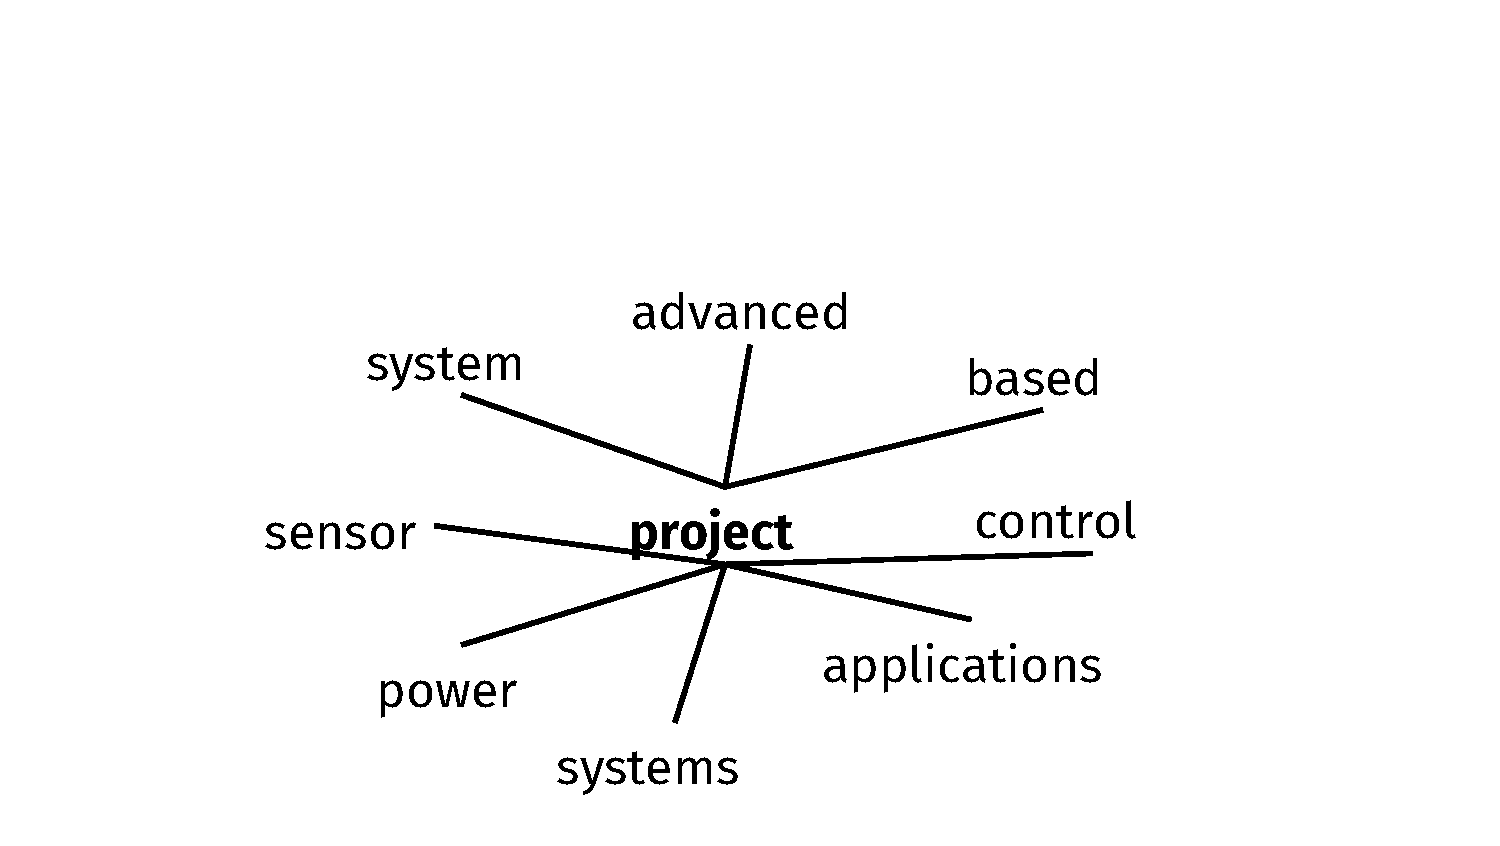
\includegraphics[width=0.8\linewidth]{images/Chapitre2/lex_net1.pdf}
\caption{Lexical network for the word \textit{project}.}
\label{fig:lex_net1}
\end{figure}


\paragraph{Syntactic Co-occurrence Networks (SCN)}
A Syntactic Co-occurrence Network (SCN) is very similar to a LCN  in the sense that both exploit the distributional hypothesis. Nonetheless, SCNs go further by leveraging  syntactic information extracted from the text. Both of the two types of syntactic parses are used: constituency-based  and dependency-based parse trees. SCNs employ, most of the time, dependency trees to create a graph that relates words according to their syntactic relations.  In Figure \ref{fig:syn_net1}, a small syntactic network is shown. In this case, the head word \textit{color} is related to the words \textit{sky} and \textit{weight} by means of a noun-modifier dependency relation  (\textit{nmod}). Other words are linked similarly according to other dependency relations.

%In the case of \cite{2013.Hope.GradedWSI}, a graph is built using syntactic dependencies.
 These networks are usually used to perform WSI employing a very similar approach to those systems using LCNs. As before, the main difference being the semantic relatedness found with one or another type of network.


\begin{figure}[!h]
\centering
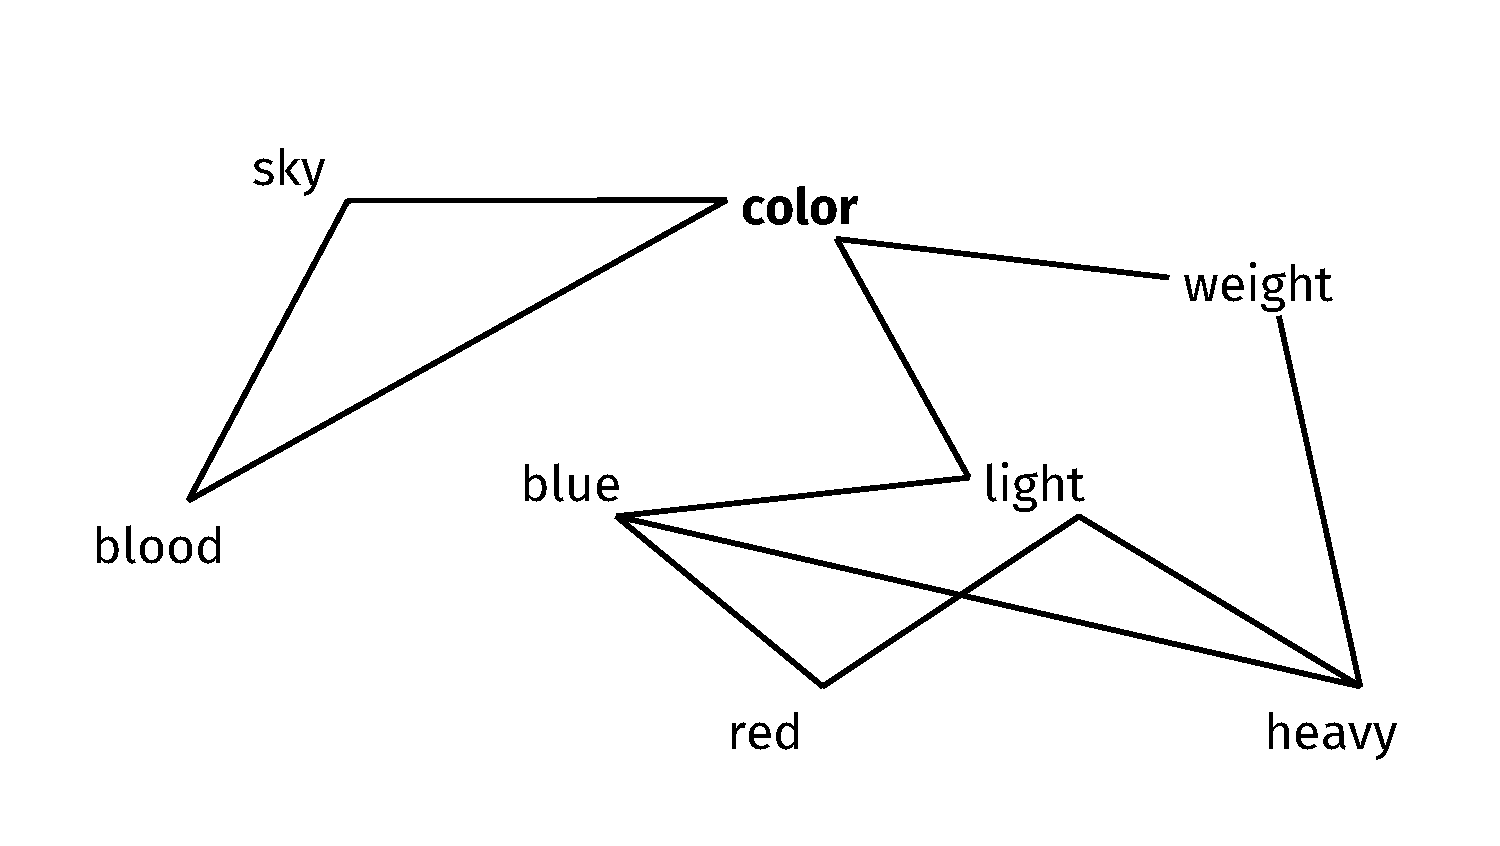
\includegraphics[width=0.7\linewidth]{images/Chapitre2/syn_net1.pdf}
\caption{Syntactic Network of the word \textit{color}.}
\label{fig:syn_net1}
\end{figure}

\paragraph{Semantic Networks}
A Semantic Network (SN) relates words, or concepts, according to well-defined semantic relations. The classical example of a SN is the renowned knowledge base Wordnet. This network, which serves also as an ontology, contains sets of synonyms (called \textit{synsets}) as vertices and semantic relations as their edges. Typical semantic relationships include synonymy-antonimy, hypernymy-hyponymy, holonymy-meronymy. However, other semantic similarities can be defined. The edges are usually not weighted, although in some cases certain graph similarity measures may be used.

\begin{figure}[!h]
\centering
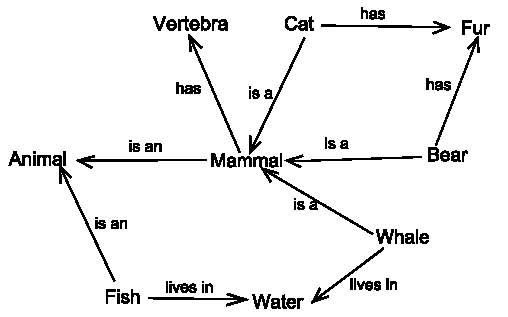
\includegraphics[width=0.7\linewidth]{images/Chapitre2/sem_net.pdf}
\caption{Semantic Network of the word \textit{mammal}.}
\label{fig:sem_net}
\end{figure}


\paragraph{Heterogeneous Networks}
Until now, we have described different types of networks with single types of nodes and relations. Lately, heterogeneous networks have been defined in order to model multi-typed information in a single structure \cite{Jiawei2009}. In reality, we could argue that syntactic-based and semantic networks are already heterogeneous on their own right, as both of them contain edges that represent different types of relations.



Without regards to their type, network-based structures are ultimately transformed into matrices before being treated computationally. Therefore, given that we are still modeling language (words), graphs suffer from sparsity just as vector space models. Indeed, data sparsity is an issue that affects the performance of knowledge discovery approaches \cite{mining12Book,PerinetH15} applied to textual data.

\section{Data Sparsity}
Representing word's contexts as multidimensional  vectors, either directly or through a graph-based structure, is indeed a straight-forward, simple and  yet powerful method to transform textual data into actionable structures. The model links  textual information, in the form of words and contexts, with the methods used in machine learning.

Nonetheless, there is an important issue that needs to be considered when dealing with vector space models: data sparsity.  A sparse data matrix has most of its entries equal to zero. Thus, the majority of the words (rows) in the corpus are described by very few contexts (columns). This is a significant problem as on the Knowledge Discovery phase of any NLP system we aim to train a learning model that will eventually predict, classify, group our words in one way ot another. If the words are represented by a limited number of context, the learning algorithms will not be able to generalize properly. Furthermore, when testing the systems, the system will not be able to handle unseen word-context co-occurrences. This will lead to reduced performance \cite{phan2008learning}.

This phenomenon is not the consequence of using vector space models per se,  as the vectors are merely a representation of  word's distribution within a text. Indeed, words tend to be distributed in a text in a very predictable fashion. In any natural language corpus, most of the words occur very few times. On the other hand, very few words occur multiple times. The consequence is that most of the entries in a co-occurrence are zero because we observe very few unique word-context co-occurrences. Put differently, words co-occur most of the times with the same words and  very few times with other words \cite{sahlgren2006word}. Given that any corpus is limited, acceptable English co-occurrences will be missing from it and their weight will be zero while they  actually happen in other corpora \cite{JurafskyM17}. To illustrate sparsity, Table \ref{tab:lexical_matrix} co-occurrence matrix contains eight words and eight contexts (each of the words), for a total of 64 entries. Among these entries, only 20 values are non-zero, and more importantly each word is only represented  by 2.5 contexts in average. While it is a toy example, and 20 non-zero entries from 64 in a matrix would hardly be considered sparse, it reflects what actually happens with larger corpora, as this problem is corpus-size independent (and even more important with smaller corpora \cite{perinet2015}). 

%\subsection{Dealing with data sparsity}
In order to deal with the distributional representation sparsity, we discuss below multiple techniques used in the literature \cite{sahlgren2006word,RatinovR09,piero2017} that aim to alleviate matrix sparsity.  In the following paragraphs we discuss explicit and implicit representations. We note that by explicit representation we refer to the classic weighted co-occurrence matrix, introduced before, where cell's values represent target word in a specific context. It is explicit in the sense that each column directly represent a context seen in the input corpus.
%


\paragraph{Implicit Representations}
These methods aim to reduce the sparsity as well as the dimension of the co-occurrence matrix while keeping latent (or implicit) features that best represent the original spaces. These techniques reduce the feature space to $k$ dimensions (usually $k$ is much smaller than the original number of columns) and thus the dimensions  are no longer directly interpretable.

\begin{figure}
\centering
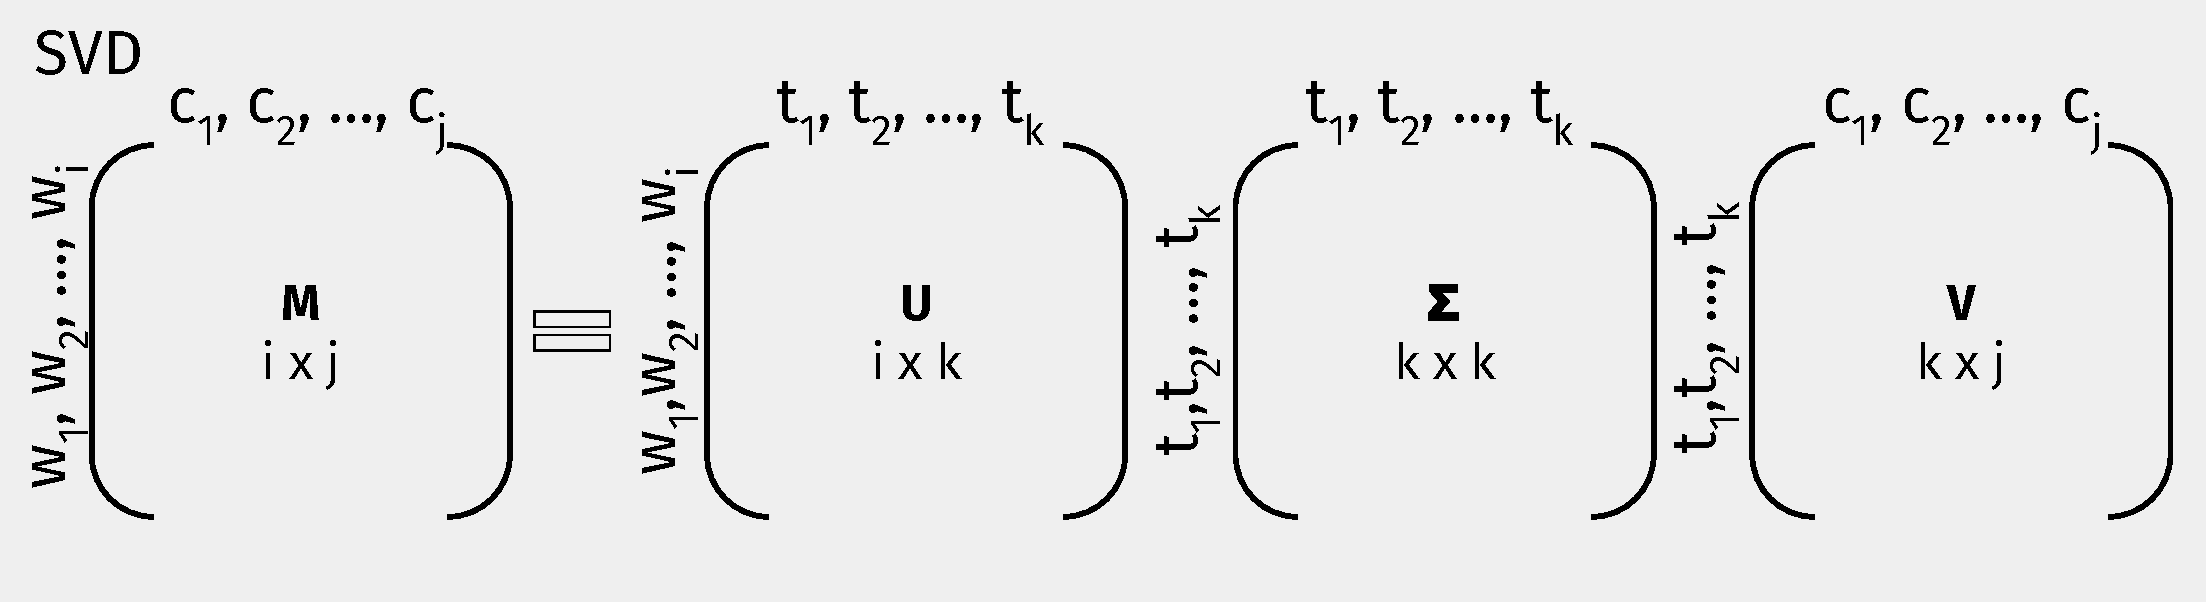
\includegraphics[width=.8\linewidth]{images/Chapitre2/svd.pdf}
\caption{Factorization of the matrix $M$ using SVD. Three matrices are generated: $U$, $\Sigma$, and $V$. $U$ is the one that really interest us, it contains $|W|$ words and $k, k<C$ columns.}
\label{fig:svd}
\end{figure}
%todo HAcer bold the matrix names

Classic examples of implicit representations include Latent Semantic Analysis and Linear Discriminant Analysis, both methods generate a word-document (terms in rows, documents in columns) co-occurrence matrix, weighted by tf-idf. Then, the matrix is reduced into a smaller dimension by means of a Singular Value Decomposition (SVD). SVD keeps the top $k$ singular values that maximize the variance among the features, $k$ being smaller than the original number of dimensions.

Recalling  the  definition of a co-occurrence matrix $M$ (where $f_{ij} \in \mathbb{R}^{W\times C}$), SVD factorizes $M$ into three matrices: two orthogonal matrices $U$ and $V$; and one diagonal, containing ordered eigenvalues $\Sigma$, and $V$, such that $M_{i\times j} = U_{i\times k}\Sigma_{k\times k}V_{k\times j}$, as shown in Figure \ref{fig:svd}. We are interested in matrix $W= U_k\Sigma_k$, as it  contains the words represented by $k$ singular values, and we thus can substitute $M$ with it. In the same fashion, we can obtain the same reduced representation for the contexts by using directly $V_k$. \cite{levy2015improving} found that, empirically, we can even dismiss the eigenvalues matrix $V_k$ in $W$ and obtain better general performance.

% todo cite allison2006another saying that data imporoves results

\begin{figure}
\centering
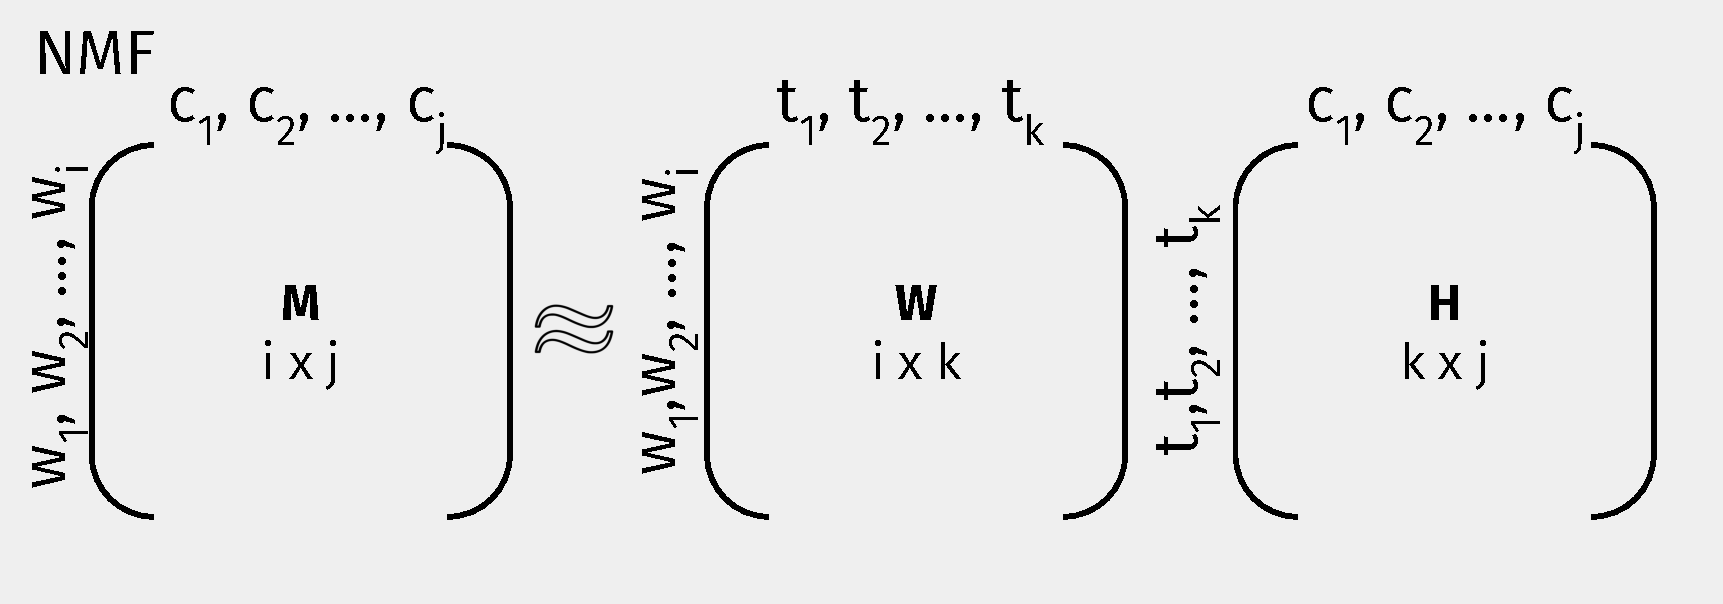
\includegraphics[width=.8\linewidth]{images/Chapitre2/nmf.pdf}
\caption{Factorization of the matrix $M$ using NMF. Two matrices are generated: $W$ and $H$. $W$ contains the words in a $k$ reduced space. $H$ contains the contexts in the reduced space.}
\label{fig:nmf}
\end{figure}

A similar approach, that of the Non-negative Matrix Factorization \cite{lee2001algorithms} (NMF)  is  also used to find latent  dimensions in the co-occurrence matrix. As shown in Figure \ref{fig:nmf}, NMF factorizes $M$ into only two matrices: $M_{i \times j} \approx W_{i\times k} H_{k\times j}$. The first matrix $W$ contains the words represented by a lower dimension $k$. On the other hand, $H$ represents the relation between the contexts and the newly induced dimensions. This procedure solves certain issues with SVD, such as containing only positive values in the factorized matrices, which is more intuitive when dealing with text, i.e., the original matrix is the result of the addition of the factorized values. Also, depending on the implementation, NMF is able to solve the Kullback-Leibler divergence (instead of the Euclidean distance, as SVD) as objective function. This measure is better suited for textual data, for example in the factorization of both lexical and syntactic co-occurrence matrices \cite{VandeCruys2011}.
 

Lastly, the most popular implicit approach nowadays is the use of distributed representations, also known more popularly as word embeddings. The goal is to represent words with a rich dense matrix and relatively few dimensions. These representations are generated from very large bodies of text, creating a regular co-occurrence matrix and calculating, via either a neural network approach \cite{bengio2003neural,Collobert2011,mikolov2013distributed} or a matrix factorization \cite{pennington2014glove,levy2014neural},  a lower dimensional and dense matrix representation. This area is fast developing, with new methods and propositions every few months. Furthermore, the community is not really certain still on which approach is better, either depending exclusively on co-occurrence frequencies and matrix factorization methods, or on sophisticated prediction approaches coupled with neural networks techniques \cite{baroni2014don,levy2015improving}.



\subparagraph{Enriched Explicit Representations}
While implicit representations modify the interpretation of the columns of the co-occurrence matrix so that they are no longer directly interpretable\footnote{Still, the meaning can be inferred to a certain level with the help of the reduced matrices.},  enriched explicit representations modify the meaning of the contexts with the addition of replacement of information to them in order to better cover a larger set of target words and thus reduce the sparsity of the matrix. More importantly, the new contexts are still \textit{natural} concepts in the sense that are still easily interpretable by us humans.




For example, leveraging the large size of the English Wikipedia corpus, the Explicit Semantic Analysis \cite{gabrilovich2007computing} aims to augment text presentation by describing words in terms of Wikipedia concepts. The method yields weighted vectors of Wikipedia concepts that best represent, according to a document ranking, an input text (see Figure \ref{fig:esa}).  The advantage of this representation is that indeed the concepts are human interpretable, not like implicit models, and it covers a very large body of information,  the Wikipedia corpus. As a downside, vectors using this representation tend to be very large, which makes dealing with them may represent a computational challenge.
% What is more, the representations are dependent on the size of the Wikipedia corpus used. 
On the other hand, vectors based on non-English versions may suffer from the reduction of textual data, as the English Wikipedia is considerably larger than most languages.

\begin{figure}
\centering
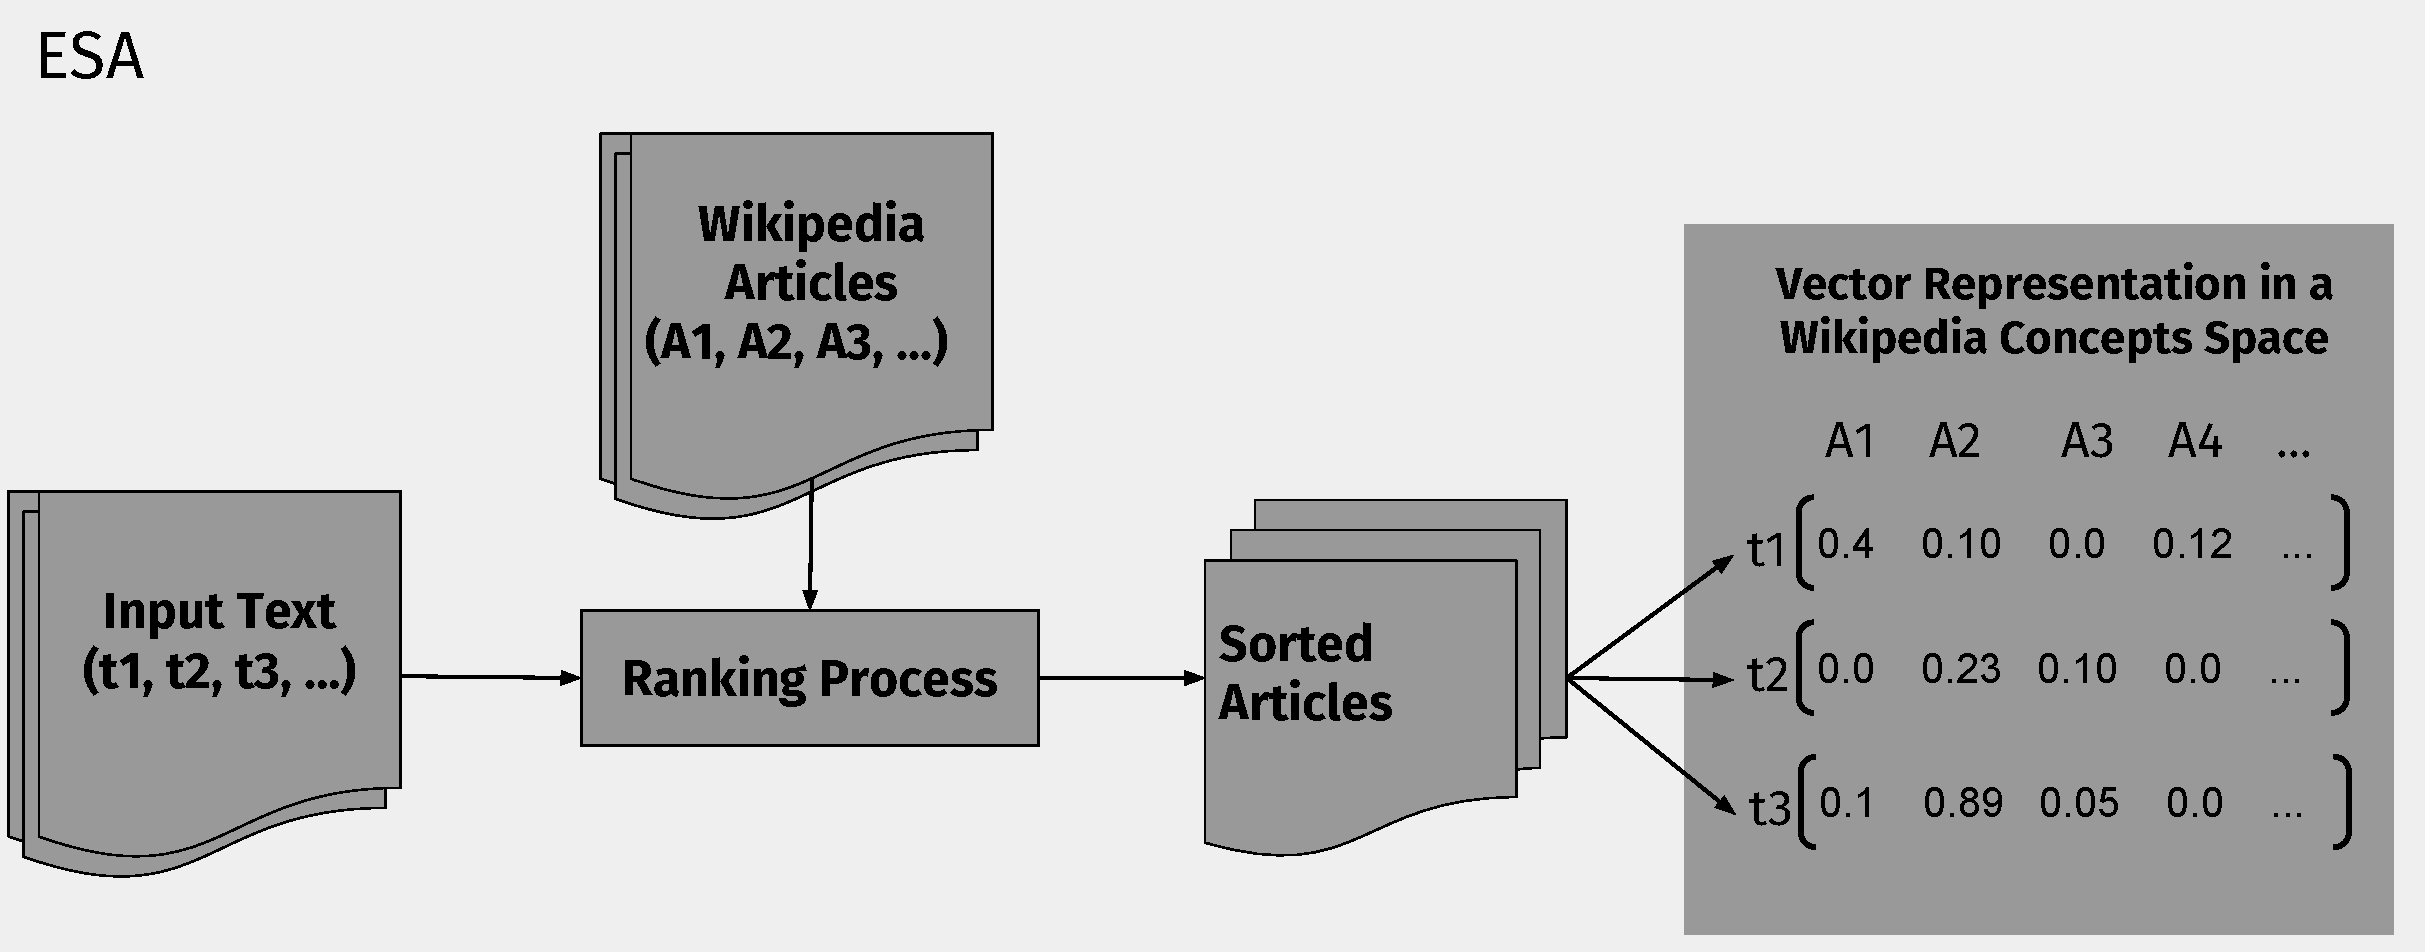
\includegraphics[width=\linewidth]{images/Chapitre2/esa.pdf}
\caption{Block description of the ESA process by \cite{gabrilovich2007computing}. The method ranks Wikipedia articles according to an input document. The document is then described by a weighted vector, where each dimension is a Wikipedia article, or concept.}
\label{fig:esa}
\end{figure}

Fusion techniques are another option to enrich and eventually densify feature spaces.  While not largely applied in the textual analysis domain as in the multimedia information retrieval and phonetics fields \cite{ozkan2010latent,Ah-PineCC15}, they represent a set of simple yet powerful methods to merge information and create more powerful representations. Indeed, these operations are based on the combination of feature spaces  to obtain representations that leverage the complementarity of the original spaces. \cite{bruni2014multimodal} has employed fusion methods to generate enriched multimedia semantic spaces while blending images and text to define the similarity among words. While feature spaces are combined, these techniques do not modify the meaning of the contexts and they remain interpretable. In this thesis, as we described in the introduction of this work, and as we will see later on, we also use these techniques to fight data sparsity by combining linguistic spaces, without resorting to other types of data. Namely,  by leveraging the properties of two distributional representations, both lexical and syntactic co-occurrences, we can get more dense and stronger  word representations. 

%todo random techniques for data spaarsity see \cite{Sahlgreen,Lenci}

\section{Conclusion}

We have introduced four axis that define the work that we carry out in this thesis. Our propositionas are based on the distributional hypothesis: we assume that words that share a common context are related. The relation is determined by the type of context: whether lexical or syntactic properties. If we choose a lexical context, the size of the window (how many words to the right, to the left) should be determined according to the ultimate goal of the NLP task at hand. This window has an effect on the semantic properties of the relatedness among words: the shorter the window, the closer we get to a synonymy similarity, i.e., we may be able to interchange words one for another and keep a coherent phrase. The larger the window, the more topical the relatedness is, i.e., words are related in a broader sense. On the other hand, when using shorter windows we indeed approach to the relatedness provided by syntactic relations \cite{sahlgren2006word}, which relate words that participate in the same syntactic dependency functions, also known as functional similarity \cite{LevyG14}. %Again, this implies that words could be substituted without losing sense within a phrase.

These contexts need to be represented computationally in order to perform some Using co-occurrence matrices, we can keep track of what words are seen with what contexts within a corpus. These counts may then be affected by some weight that determines the relevance of said co-occurrences in terms of uniqueness in terms of the whole set of co-occurrences found. Once these word's vectors are created, we can thus finally calculate a degree of relatedness between them by employing vector similarity metrics, notably the cosine similarity (for real-valued vectors) and Jaccard (binary valued vectors) metrics.

While matrices are the fundamental structure used in computational operations, we can model the links among words intuitively with graph-based structures. Indeed, by modeling text as graphs we gain access to  established graph-theory techniques which helps us elucidate the inner structure of textual data. 	

Whether its vector based or graph based, a textual, explicit, and distributional representation will be sparse. There are too many words in a text and its assured that, while they could occur in other texts, they will not occur in a single text. This becomes an important problem with NLP systems: words are described by only a small set of features.

In the following chapter we describe our two first propositions which address the issue of using heterogeneous information to represent a term and alleviating the data sparsity that comes with such types of textual representations.


%
	

%\section{Graph-based Models}
%
%
%\section{Word Sense Induction and Disambiguation}
%\section{Named Entity Recognition}

%\section{Sequential Classification: Structured Perceptron}
%\section{Clustering: Spectral Clustering}

%++++++++++++++++++++++++++++++++++++++++++++++++++++++++++++++++++++++++++++++++++++++++++++++++++




\chapter{Fusion Enriched Hypergraph Linguistic Model}
\label{chap:ling_net}
\begin{abstractchap}
In the previous chapter we presented the theoretical notions used to represent text with a distributional approach, that is, the parameters, the models to implement them  and the problems that naturally arise from these kinds of representations. In this chapter we introduce and define the first set of our contributions. Briefly, we present a linguistic framework to represent textual data. Feature fusion techniques are then applied over this network in order to better leverage the data contained in it while addressing the sparsity issue.

We organize this  chapter  in four parts: we present a brief state of the art on how the information contained in linguistic graphs is used for WSD/WSI and NER. Secondly, we introduce our model. Thirdly, we present  the method used to combine the data held in our mode, specifically using feature fusion techniques. Finally, we materialize the proposed model by transforming an English Wikipedia based corpus into our proposed framework.
\end{abstractchap}
\minitoc

\section{Introduction}

We have covered the details concerning the parameters regarding the construction of a distributional representation model, as well as its challenges.
The challenges that we will address in this chapter are two: (1) how to organize heterogeneous textual information within a single linguistic resource, and (2), how to leverage said information to obtain complementary representation spaces, while taking into account the feature sparsity issue that is characteristic of textual data.


The first two contributions of this thesis are contained in a fusion enriched hypergraph linguistic model proposition. The model consists on two components which address two research questions each: the issue of making sparsity less severe and leveraging different types of features  by using a single feature representation space. We will describe our motivations and its characteristics in the following paragraphs. We can see the block diagram of the ensemble of our propositions  on Figure \ref{fig:maindiag}. There, we can observe our enriched linguistic model proposition, comprising our first two propositions, which is the focus of this chapter, as well as the instantiation of said model using a Wikipedia based corpus. %On the bottom, we show the application of said model in NLP tasks, described thoroughly in Chapter \ref{chap:wsd}.

The model we present here entails three  important characteristics: firstly, the possibility to leverage different\footnote{We use three in our model definition: syntactic, lexical  and what we will call standard features (explained later on).} types of information.  Secondly, as the words will be linked together, there is an inner structure that will emerge from the model and which we exploit in our experiments. Thirdly, given that we treat unstructured text data, the relations (or features)  between words are sparse, this is alleviated by combining features via fusion techniques.  The three of them are addressed with our propositions. 
In the following chapter, we test the practicality of our proposal with well-established tasks and related evaluation corpora, which we use as benchmark input data in our experiments. 

Our network is based on the distributional hypothesis, as described in the previous chapter.  As co-occurrence features, we select both lexical and syntactic contexts, indeed creating a linguistic resource that hold both types of information in order to get a complementary insight of words' relations. Our network sets a lexical window, a co-occurrence weighting, and the definition of similarity between vectors according to two semantic NLP tasks 
we treat in the following: word sense induction and disambiguation and named entity recognition. Nonetheless, the parameters chosen can be easily changed. Regarding representation, we base our model on a graph-based structure which holds the words as nodes and the linguistic relations as edges. Being able to use the structure of the graph is useful to solve NLP semantic tasks \cite{nastase2015}. The following paragraphs will describe this structure in detail.   
%
%As stated before, both types of textual contexts entail the need to alleviate the feature-matrix sparsity issue. At the same time, we want to leverage these contexts as it is significant to our goals. In this sense, we use fusion techniques form the multimedia analysis literature to deal with both sparsity and the heterogeneity of our contexts.

%The next chapter introduces our first contribution, a linguistic network as a resource for solving NLP tasks.




\begin{figure}
\centering
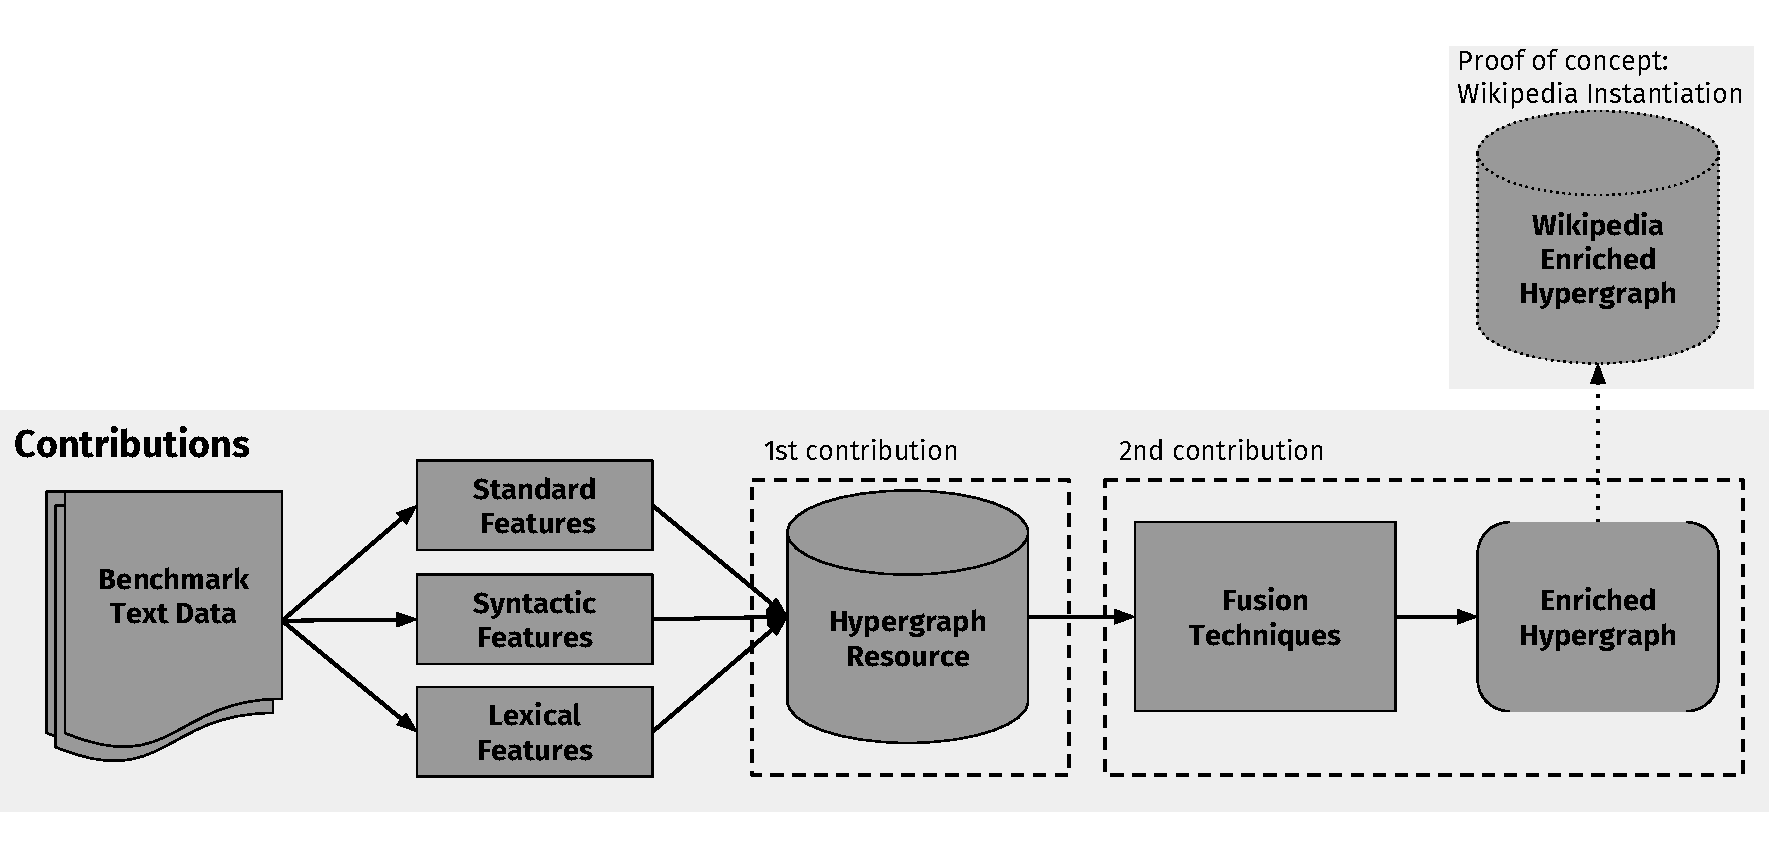
\includegraphics[width=1\linewidth]{./images/Chapitre3/main_diag_p1.pdf}
\caption{Modular description of the first two contributions of this work: an enriched hypergraph resource.}
%  We see the elements of the fusion enriched hypergraph model we propose and its proof of concept instantiation.} 
%Also, at the bottom, the NLP tasks applications based on said model: word sense induction and disambiguation and named entity recognition.}
\label{fig:maindiag}
\end{figure}

In order to contextualize our proposition, we begin with the state of the art on how linguistic networks are employed in the literature. We are interested in those networks previously covered: lexical, syntactical and semantic co-occurrence networks. We give emphasis to two aspects: how the inner structure is used to solve the tasks at hand, and what type of graph-based algorithm is used. The literature on graph-based approaches for NLP is vast, we thus focus specifically on semantic tasks, notably Word Sense Induction and Disambiguation, and Named Entity Recognition. We chose these two tasks as we focus on both of them for the rest of our contributions. Afterwards, we introduce our model, how to build it  and its properties. We focus on the description of hypergraphs and how they allow us to join together different linguistic networks. Next, we introduce the concept of fusion techniques used to combine the linguistic features and obtain an enriched representation.

In that sense, this chapter presents a word representation model based on a generalization of graphs (we employ hypergraphs) that contains different types of linguistic data to characterize the terms (or words) contained within.  These representations are then combined with fusion techniques in order to ideally get an enriched and complementary feature space for each word. Finally, as a proof of concept, we describe the characteristics of the transformation of an English Wikipedia-based corpus into the framework we propose, a hypergraph model and its single enriched representation produced via fusion techniques. We show an example of the results produced by these fusion methods.

%The materialization of the proposed model allows us to computationally test the advantages as well as to discover the limitations of the proposed framework
%In the following chapter, we show in our experiments that this is indeed the case. 
.

\section{Linguistic Networks in Semantic NLP Tasks}\label{sec:ling_net_nlp}



We present here an overview of linguistic network's related work. We discuss what and how different methods are used with language networks to extract knowledge from their structural properties. Finally, we discuss the limitations of the current propositions and the advantages of the model we propose.
%\minitoc



\paragraph{Using Lexical Co-occurrence Networks}

Lexical Co-occurrence Networks (LCN) are  popular  since they do not require any special treatment to obtain them, just the input corpus. It is then natural that truly-unsupervised\footnote{Without the need of human-crafted semantic networks.} word sense induction approaches leverage these type of networks, and in return, the distributional hypothesis, to automatically discover senses for a given target word. That is why several WSI methods \cite{2004.Veronis,2007.Klapaftis.UoY,2010.Navigli.InducingWordSenses.Triangles,2008.Klapaftis.WSIUsingCollocations,2011.DiMarco.Navigli.ClusteringWebSearch,2011.Jurgens.WSICommunityDetection} are tightly related to LCNs. 
The cited works use a LCN as described before while other works such as \cite{2007.Navigli.GraphConnectivity,2014.Tao.Qian.LexicalChainHypergraphWSI} represent, as we do, the co-occurrence by means of a hypergraph scheme. In short, a hypergraph structure is a graph generalization where an edge (called hyperedge) can link more than two vertices per edge and thus it is able to provide a more complete description of the interaction between several nodes \cite{estrada2005}. In that sense, in  \cite{2014.Tao.Qian.LexicalChainHypergraphWSI} they make use of this type of representation to solve the task of word sense induction. Briefly, in this task we have to determine a set of senses for a given target word in a corpus, according to its context (a context here being usually a paragraph where the target word occurs). In their paper, given an input document with several context instances for each target word, they first extract lexical chains (set of semantically related words) from the contexts using a topic-modeling based technique. Secondly, a hypergraph is built where the vertices represent words and the hyperedges link two or more words if they exist in the same lexical chain. Thirdly, the hypergraph is clustered and groups of words are found which are considered to be the senses of the target word. Lastly, to assign these senses to each target word instance, they consider each sense as a vector, whose dimensions are each word in the corresponding cluster and its weight determines its level of co-occurrence  with the target word. The sense assignation is done by determining the similarity between sense vectors and a vectorial representation of each target word instance.

Generally, WSI systems generally perform four steps \index{WSI steps}. Given an input text with a set of target words and their contexts (target words must have several instances throughout the document to cluster them), the steps are the following:

\begin{enumerate}
\item Build a LCN, assigning tokens as nodes and  establishing edges between them if they co-occur in a given context (usually if they both appear in the same sentence),
\item Determine the weights for each edge according to a frequency metric,
\item Apply a graph clustering algorithm. Each cluster found will represent a sense of the polysemous word, and
\item Match  target word instances with the clusters found by leveraging each target word context. Specifically, assign a cluster (a sense) to each instance by looking at the tokens in the context.
\end{enumerate}

As with semantic networks, not only WSD or WSI can be solved with LCNs. Finding semantic associated terms in a corpus is a critical step in several NLP systems. This task is solved in the system proposed by \cite{2011.Haishan.AHypergraphbased}. They also use a LCN although instead of a co-occurrence graph, they also employ a co-occurrence hypergraph, where nodes represent words and edges describe co-occurrence at the paragraph level.  In this work, they use such structure to find related terms in a given corpus. In order to do it, they mine the hypergraph as in a frequent itemsets problem, where the items are the words from a text. The method consists in first finding similar itemsets by means of measuring similarity between nodes. Once the 2-itemsets are found, they induce a graph from the original hypergraph by drawing edges between nodes that have a similarity superior to an arbitrary threshold. Lastly, in order to find $k$-itemsets ($k > 2$), the find either complete or connected components in the induced graph. 



As with WSD, while the LCNs used are mostly the same among approaches, there are certain moving parts that make up the difference between WSI approaches. The most common differences that can arise are:

\begin{itemize}
\item The clustering algorithm to find senses in the LCN graph.
\item The technique used to match context words to clusters.
\item The weight used in the graph edges.
\end{itemize}



\paragraph{Using Syntactic Co-occurrence Networks}

A network representation that is on the border line between being a LCN and a SCN is that of \cite{2013.Bronselaer.TextAnalysisWithGraphs}. They  propose a graph document modelization. In their network, nodes represent words and edges their co-occurrence, as any LCN. Still, their graph resembles a SCN because the edges may represent one of three types of words: either prepositions, conjunctions or verbs. As a result,  they need to first extract syntactic information from a document, namely the part-of-speech tags of each word. They find the most relevant words of a given text by ranking the nodes of the graph. The words that best represent a document can be used to summarize it, as they show in their work.

Approaches based on SCN are rarely used in WSD or WSI systems, and therefore they are an interesting research avenue to explore.




\paragraph{Using Semantic Networks}

Word sense induction is indeed a task usually solved using semantic networks, specially WordNet (and to a lesser extent, BabelNet) \cite{2004.Mihalcea.SemanticNetworkPageRank,2007.Sinha.Mihalcea.Unsupervised,2007.Tsatsaronis.WSDwithSpreading,2007.Navigli.GraphConnectivity,2008.Agirre.Multilingual,2008.Klapaftis.WSIUsingCollocations,2009.Agirre.PersonalizedPageRankWSD,2010.Klapaftis.WSD.WSD.HierarchicalGraphs,2010.Siberer.GraphCooccurrenceWSD,2014.Moro.Navigli.EntityLinking_WSD}. Given an input text with a set of ambiguous target words to process, these approaches follow a two-step algorithm:
\begin{enumerate}
\item Link target words (usually nouns, skipping stop-words and functional words) with their corresponding  sense (or synset in the case of WordNet-like dictionaries) and extract their vertices and edges into a new, smaller, SN. 
\item Apply a node ranking technique, usually a random-walk-based method, and select, for each ambiguous word in the input text,  its top ranking synset node as the correct sense.
\end{enumerate}

The amount of edges a SN has grows depending of the size of the version of WordNet used or the level of polysemy of a given word. In order to avoid redundancy or contradiction between  linking nodes, \cite{2004.Mihalcea.SemanticNetworkPageRank,2007.Navigli.GraphConnectivity} applied pruning techniques to avoid \textit{contamination} while calculating ranking metrics in order to define a pertinent sense. Regarding edge similarity measures,  in  \cite{2007.Sinha.Mihalcea.Unsupervised, 2007.Tsatsaronis.WSDwithSpreading} they test some metrics individually and also combined. They found that the best results are indeed obtained when multiple metrics are used at the same time.

%Other semantic tasks can also be solved using a SN. For example, Entity linking \cite{2014.Moro.Navigli.EntityLinking_WSD}. In their work, they leverage the BabelNet LKB to jointly disambiguate and link polysemous words to Wikipedia articles. 

Concerning the measure of semantic affinity between two terms, in \cite{2009.Yeh.Wikiwalk} they quantify word similarity by means of projecting them into a Wikipedia space. First, they represent each word by a vector representing its most pertinent pages,  and then they calculate a vectorial similarity measure between them.

%In \cite{2013.Matuschek.Gurevych.Dijsktra.WSA} they propose a technique that aligns SNs, i.e., they link senses from two different networks. This task is called word sense alignment. Several SNs are used (WordNet, Wikipedia, Wiktionary, etc.) thus nodes can represent synsets, articles, or concepts. The links may depict semantic relations or may be links joining two concepts or pages together. Their approach aims to find the shortest path between nodes of any two given SNs while leveraging already existing links between  equal concepts found in both SNs.



Finally, extracting entities from text can also benefit from the use of SNs. The work proposed by  \cite{2013.Kivimaki.AGraph-BasedApproach} aims to extract technical skills from a document. Again, using Wikipedia as SN, they first represent each article and the input document in a token vector space model.  Next, they find the document top 200 similar pages by calculating the cosine similarity between the document and each page. This serves to extract a Wikipedia subgraph which is used to calculate the most relevant pages for the entry document. Finally, the top pages are filtered by means of selecting those articles that actually represent a skill using a fixed list of skill-related tokens. Once again, the nodes represent Wikipedia articles and the edges the hyperlinks that join them.


The cited methods vary in how they make use of their SN, not so much in the network per se. These differences boil down to three aspects:
\begin{enumerate}
\item Type of relationship implied by the edges linking the nodes of the network, 
\item The algorithm used to rank the nodes after the semantic network is built, and
\item The weight assigned to each edge.
\end{enumerate}

\paragraph{Using Heterogeneous Networks}

Even though this kind of structure seems to open new avenues of research in the semantic analysis domain, only few explicitly take advantage of them, as is the case of \cite{2013.Saluja.Graph-BasedUnsupervisedLearning}. In their approach, they build a graph that links together features with words, and discover similarity measures that leverage the multi-typed nature of their network.


\subsection{Algorithms used in Linguistic Networks}

We have discussed until now the different types of networks from a content point of view. In this subsection, we address the details of the graph-based algorithms used to solve semantic NLP tasks. In this section we cover the details of four different types of graph algorithms.

%\paragraph{Notation}
%In this section we will be referring to a connected undirected graph, which we denote by $G = (V,E,W)$. The graph $G$ has vertex set $V$, edge set $E$ where $|V|=n$, $|E|=m$, and the matrix $W\in\mathbb{R}^{n\times n}$, with $w_{u,v} \geq 0$, defines any kind of weights in the graph.


\paragraph{Edge Weights}

We begin by describing the metrics used to determine similarity between nodes, usually stored as edge weights. As stated in the previous sections, most of the metrics are frequency based, specially when dealing with LCNs. The main idea of these measures is to assign a weight that decreases as the association frequency of the words increases. Among these measures, the most popular are the Dice  coefficient \cite{2010.Navigli.InducingWordSenses.Triangles,2011.DiMarco.Navigli.ClusteringWebSearch,2013.DiMarco.Navigli.ClusteringGraph-BasedWSI}, normalized pointwise mutual information \cite{2013.Hope.GradedWSI}, and a graph-adapted tf-idf variant \cite{2007.Tsatsaronis.WSDwithSpreading} which aims to give importance to frequent edges while also favoring those that are rare.

Edge weights can also be calculated when the vertices of a network do not represent words. Such is the case of \cite{2010.Klapaftis.WSD.WSD.HierarchicalGraphs}, where nodes represents a target word context (set of tokens around an ambiguous word). This time the Jaccard index is used to quantify similarity between them while considering how many words are shared between a pair of context nodes.

When the nodes represent synsets (or concepts), certain approaches leverage only the intrinsic nature of the network connections, leveraged by random walk algorithms, without explicitly using  weighted edges \cite{2004.Mihalcea.SemanticNetworkPageRank}. 
 On the other hand, there are techniques that assign a frequency-based weight to represent the importance of a semantic relation, particularly those found in the reviews  by \cite{2007.Sinha.Mihalcea.Unsupervised,2007.Navigli.GraphConnectivity}, where several weights are tested.

A  more sophisticated approach to edge weighting is proposed in \cite{2013.Saluja.Graph-BasedUnsupervisedLearning} where they employ  custom-defined functions in order to learn the most appropriate edges' weights for a given set of seed vertices inside a network. The main idea  is to enforce \textit{smoothness} \index{smoothness} (keeping two nodes close if they have related edges) across the network.

As a way to rank edges according to their importance, the ratio of triangles (cycles of length 3), squares (cycles of length 4), and diamonds (graphs with 4 vertices and 5 edges, forming a square with a diagonal) in which an edge participates are calculated \cite{2010.Navigli.InducingWordSenses.Triangles,2013.DiMarco.Navigli.ClusteringGraph-BasedWSI}. Once the top edges are found, they create a subgraph containing only these edges (and its corresponding vertices).

Finally, instead of applying weights to edges, a case where  nodes are weighted can be found in \cite{2013.Kivimaki.AGraph-BasedApproach}. They measure and remove popular nodes in order to avoid their bias during the application of their random walk approach.




 

\paragraph{Graph Search} \index{Graph Search}
Usually, in a WSD approach, the first step to follow is to build a graph from a LKB. The goal is to explore the semantic network and find all the senses linked to  those found in the context of an ambiguous word. Aside from custom search heuristics applied by certain works \cite{2006.Agirre.TwoGraph-basedAlgorithms,2007.Sinha.Mihalcea.Unsupervised,2009.Agirre.PersonalizedPageRankWSD}, researchers also use well-known graph techniques such as depth-first search \cite{2007.Navigli.GraphConnectivity}, breadth-first search \cite{2008.Agirre.Multilingual} and even the Dijsktra  algorithm to find the group of closest senses in the network \cite{2013.Matuschek.Gurevych.Dijsktra.WSA}.


\paragraph{Node Connectivity Measures}\label{sec:connectivity_measures} \index{Node Connectivity Measures}
A Connectivity Measure (CM) determines the importance of a node in a graph according to its association with other nodes. In most cases its value ranges from zero to one, where the 0 indicates that the node is of minor importance while 1 suggests a relatively high significance. Nowadays, the most widely used  measures are those based on random walks.

A Random Walk (RW) can be simply defined as the traversal of a graph beginning from a given node and randomly jumping to another in the next time step.
% It is similar to a Markov chain process, the difference being that in a Markov chain the next step node is chosen to according to a certain distribution.  

PageRank \cite{Brin1998} \index{PageRank}, the popular random walk based algorithm is used commonly in WSD. The recursive intuition of PageRank is to give importance to a node according to the PageRank value of the nodes that are connected to it. %Formally, the vector PageRank holding values for each node in $v \in V$ is calculated as: $PR(v) = \alpha\sum_{u,v\in E}{\frac{PR(u)}{outdegree(u}} + \mathbf{v}(1-\alpha)$, where $ \alpha  $ is a dumping factor to control the jumps a random walker will make; and $ \mathbf{v} $ is the relevance vector for each node has in $G$. In classical PageRank, the values of  $\mathbf{v}$ are uniformly set to $\frac{1}{n}$ for all nodes in $|V|$. 
Nonetheless, as a regular random-walk algorithm, in PageRank the probability distribution to change from a node to another is uniform. In such case, the jumps a random walker performs depend solely on the nature of the graph studied. Among the approaches surveyed, those that use the most PageRank are those that solve word sense disambiguation \cite{2004.Mihalcea.SemanticNetworkPageRank,2006.Agirre.TwoGraph-basedAlgorithms,2007.Navigli.GraphConnectivity,2010.Siberer.GraphCooccurrenceWSD}. 
%
These approaches make a conventional use of PageRank: they apply it and rank nodes to select the most appropriate senses for ambiguous words. Still, there are some improvements over the classical use of PageRank in WSD. Some techniques employ a different version of PageRank called Personalized PageRank (or PageRank with restart \cite{Murphy2012} or PPR) \index{Personalized PageRank (PPR)} were a random walker may return to a specific starting node with certain probability rather than jumping to a random node. This formulation allows researchers to assign more weight to certain nodes. For example, in \cite{2009.Agirre.PersonalizedPageRankWSD} they are able to use the complete Wordnet graph as their SN. They do this by directly adding context words of a polysemous token into Wordnet and then giving a uniform initial distribution to only these nodes. In this way, they force PageRank to give more importance to the context words without the need of extracting a subgraph from the SN. In \cite{2014.Moro.Navigli.EntityLinking_WSD} they apply the same technique to obtain a \textit{semantic signature} of a given sense vertex. After applying PPR, they obtain a frequency distribution over all the  nodes in the graph. The so-called semantic signature consists in those nodes that were visited more than an arbitrary threshold and that best represent an input sense node.

There are other methods which share the properties of random walk approaches. In  \cite{2007.Tsatsaronis.WSDwithSpreading,2013.Kivimaki.AGraph-BasedApproach} they apply a method known as spreading activation. This algorithm aims to iteratively diffuse the initial weights of a set of seed nodes across the network. Specifically, once a weighted semantic network is built, they \textit{activate}  the nodes representing the context senses, assigning a value of 1, while \textit{deactivating} the rest by setting them to 0. They determine the most pertinent senses to the input nodes by storing, for each of them, the last active sense node with the highest activation value. 

Beyond WSD and into the task of determining word similarities, we found the work of \cite{2009.Yeh.Wikiwalk}, where they calculate a semantic similarity between a pair of words while leveraging a Wikipedia SN. For each word, they  apply PPR to find the articles that best represent a word. 
%They set the initial distribution in such a way that the articles that best represent each word have a higher probability than the rest of nodes. 
In \cite{2013.Saluja.Graph-BasedUnsupervisedLearning}, they also employ PPR to find synonym words given a word-similarity matrix and a new unknown word (also known as out-of-vocabulary word). They link the new word to its corresponding feature nodes and they normalize the similarity matrix to use the weights as probabilities and thus bias the random walk. In \cite{2013.Kivimaki.AGraph-BasedApproach} they use centrality measures to determine the most relevant nodes in a SN and then, in contrast with most approaches, remove them from the graph in order to not bias their graph algorithms.
%

With regard to other CMs, there are  more elementary alternatives to determine the importance of a node. For example, the approaches of  \cite{2004.Veronis,2007.Klapaftis.UoY,2011.Haishan.AHypergraphbased,2013.Bronselaer.TextAnalysisWithGraphs,2014.Moro.Navigli.EntityLinking_WSD} successfully use the degree of a node, or other metric, to determine its importance in a network.

\paragraph{Graph Clustering/Partitioning} \label{par:partitioning_clustering} \index{Graph Clustering/Partitioning}

Graph clustering is defined as the task of grouping the vertices of a graph into clusters while taking into consideration its edge structure \cite{Schaeffer2007}. As previously mentioned, graph-based word sense induction relies most importantly in the graph clustering step where the actual senses of a word are inferred. 

In this subsection we also consider  subgraph extracting techniques which are exploited to find separated groups of words and thus induce senses. In this context we found the approaches of \cite{2004.Veronis,2010.Siberer.GraphCooccurrenceWSD}. These systems make use of both the Minimum and Maximum Spanning Trees algorithms (MinST and MaxST, respectively) as a final step to  disambiguate a target word given its context.  Meanwhile, both \cite{2011.Haishan.AHypergraphbased,2014.Tao.Qian.LexicalChainHypergraphWSI}  use the Hypergraph Normalized Cut (HCT) approach, a hypergraph clustering method based on minimum cuts, to induce senses.

Most of the reviewed approaches employ state of the art techniques \cite{2008.Klapaftis.WSIUsingCollocations,2010.Klapaftis.WSD.WSD.HierarchicalGraphs,2011.Jurgens.WSICommunityDetection,2013.Hope.GradedWSI}. Specifically, they utilize Chinese Whispers (CW) \index{Chinese Whispers (CW)} \cite{biemann2006chinese}, Hierarchical Random Graphs (HRG) \index{Hierarchical Random Graphs (HRG)} \cite{clauset2008hierarchical}, Link Clustering (LC) \index{Link Clustering (LC)} \cite{ahn2010link}, and MaxMax (MM) \index{MaxMax(MM)} \cite{hope2013maxmax} respectively. 

Briefly, CW is a randomized graph-clustering method  which is time-linear with respect to the number of edges and does not need a fixed number of clusters as input. It only requires a maximum amount of iterations to perform. HRG, being a hierarchical clustering algorithm, groups words into a binary tree representation, which allows to have more in-detail information about the similarity among words when compared to flat clustering algorithms. Regarding LC, instead of clustering nodes, this procedure groups edges. Thus it can identify contexts related to certain senses, instead of finding groups of words as most approaches do. Finally, MM, is able to assemble words into a fixed cluster (hard clustering) or allow them to be in several groups at the same time (soft clustering). It shares certain characteristics with CW:  they are both methods that exploit similarity within the local neighborhood of nodes and both are time-linear. Nonetheless, a key difference is that CW is not deterministic, while MM is, thus MM will always find the same clustering result for the same input graph.

Another common clustering approach to automatically induce word senses \cite{GoyalH14,Song16} is spectral clustering \cite{Shi2000} \index{spectral clustering}. Some advantages of this method include that it is simple to implement and often outperforms other clustering methods as well as being able to work directly with graph and non-graph data \cite{Luxburg2007}.
%
The algorithm consists in projecting the normalized Laplacian \index{Laplacian} of an affinity (or similarity) matrix (adjacency matrix in the case of graph data) on its $k$ first eigenvectors. The lower-space projection allows for an easier separation, for example with $k$-means, in order to find the  group membership of each original data point. 

%  The adjacency matrix is used to compute a normalized graph Laplacian
%    whose spectrum (especially the eigenvectors associated to the
%    smallest eigenvalues) has an interpretation in terms of minimal
%    number of cuts necessary to split the graph into comparably sized
%    components.
%
%    This embedding can also 'work' even if the ``adjacency`` variable is
%    not strictly the adjacency matrix of a graph but more generally
%    an affinity or similarity matrix between samples (for instance the
%    heat kernel of a euclidean distance matrix or a k-NN matrix).

Indeed, the Laplacian of an affinity matrix can be used to represent several properties of the inherent structure within the data. Specifically, in the case of a graph, it tells us about the number of connected components through its  set of eigenvalues, specially the eigenvectors associated to the smallest eigenvalues, which synthetically represent the data.

The normalized Laplacian of an affinity (symmetric and positive) matrix $W\in \mathbb{R}^{n\times n}$, with $w_{ij} = w_{ji} \geq 0$, is defined as: 
\begin{equation}\label{eq:norm_laplacian}
\mathcal{L} = I - D^{-1/2}WD{-1/2}
\end{equation}

where $I$ is the identity matrix and $D$ is the degree matrix of $W$. $D$ is defined as the diagonal matrix with the degrees $d_1 ,\dots,d_n$ on the diagonal. As $W$ may not be an adjacency matrix, we define the degrees of each row in the matrix as: $d_i=\sum_{j=1}^{n}{w_{ij}}$.

Given a  symmetric and positive similarity matrix $W \in \mathbb{R}^{n \times n}$, and a number of desired clusters $k$, the steps required to perform spectral clustering are:

\begin{enumerate}
\item Obtain the normalized Laplacian $\mathcal{L}$ as indicated in Equation \ref{eq:norm_laplacian}.
\item Obtain the first $k$ eigenvectors $u_{1\dots k}$ of $\mathcal{L}$.
\item Store said eigenvectors as columns in a matrix $V \in \mathbb{R}^{n \times k}$. This matrix is akin to a lower-dimension projection of the original similarity matrix $W$.
\item Cluster the points in $V_i$ with $k$-means. The clusters found and their members correspond to the cluster of the spectral algorithm.
\end{enumerate}

Special attention must be given to the input matrix $W$ as it must be indeed a symmetric affinity matrix in order to ensure the proper behavior of this method \cite{Luxburg2007,GoyalH14}.



\paragraph{Supervised Sequential Classification}\label{sec:perceptron} \index{{Supervised Sequential Classification}}

In order to determine the correct set of tags that identify the words within a phrase, sequential NLP tasks such as NER, are usually solved by using supervised structured algorithms. In particular, we focus on the  structured perceptron \index{structured perceptron} by \cite{Collins2002} sequence labeling algorithm. The general intuition of this method is introduced below. We chose this method as it is relatively simple and performs as well as more complex probabilistic approaches (e.g., conditional random fields, hidden Markov models)  \cite{Daume2006,daume2012course}. 


Like  the well-known perceptron algorithm, the structured perceptron is an online method that learns to classify one example at a time. The goal of this algorithm is to determine a label for each structured input. Formally, for an input $x \in \mathcal{X}$, we want to predict a class $\hat{y} \in \mathcal{Y}$ that maximizes the following matrix product: 

\begin{equation}
\hat{y}= \argmax_{\hat{y}\in \mathcal{Y}}w\cdot \Phi(x,\hat{y})
\end{equation}
where $\Phi(x,\hat{y})$ is the vector of representing  the feature space of input  $x$ with respect to each of the  possible labels $\mathcal{Y}=\{1,\dots,\textit{K}\}$. Indeed,  $\Phi(x,\hat{y})$ indicates a certain level of compatibility between input $x$ and each label $y$. 

We learn $w$ as a weight vector which considers each feature in regard to each class. As with the classic perceptron, $w$ is updated if the predicted $\hat{y}$ is different to the true label $y$, as follows: 

\begin{equation}
w \leftarrow w+\Phi(x,y) - \Phi(x,\hat{y})
\end{equation}

The algorithm for the structured perceptron is shown in Algorithm \ref{alg:struct_perc}.  For each input, we obtain its predicted class and determine whether it is equal to the true label. If it is not the case, we update the weight vector.

\begin{algorithm}[htp]
\SetAlgoLined
\KwIn{Data $x \in \mathcal{X}$}
\KwIn{True labels  $y \in \mathcal{Y}$ }
\KwIn{Max number of iterations $MaxIteration$}
\KwOut{A vector of lerned weights $w$}
\For{$Iteration=1\dots MaxIterations$}
{
	\ForEach{$(x,y) \in \mathcal{X},\mathcal{Y}$}
	{
	
		$\hat{y}= \argmax_{\hat{y}\in \mathcal{Y}}w\cdot \Phi(x,y)$
		
		\If{$\hat{y}\neq y$}
		{	
			$w \leftarrow w+\Phi(x,y) - \Phi(x,\hat{y})$
		}
	}
}

\Return{$w$}


\caption{Training phase of the Structured Perceptron}
\label{alg:struct_perc}
\end{algorithm}


The main issue with this algorithm is the computation of $\argmax_{\hat{y}\in \mathcal{Y}}w\cdot \Phi(x,\hat{y})$ in line 3 of Algorithm \ref{alg:struct_perc}. As said before, we are looking for the sequence of labels $\hat{y}$  that maximize this product. This implies a very large search over all the possibilities that grows exponentially with the number of possible tags $\mathcal{Y}$. If we consider a phrase with $L$ words, and a tagset of $k$ labels, the total number of possibilities to explore would be $L^k$. For example, for a phrase with 10 words, and 5 labels, we would need to explore a space of $10^5=100,000$ possibilities. This exploration then tends to be computationally unfeasible for a large number of phrases and/or a larger number of words per phrase.

In order to address this problem, another familiar  algorithm is employed: the Viterbi decoder\index{Viterbi decoder}. Briefly, this method calculates the optimal set of labels for each input, by determining the maximum path (or sequence of labels) through a lattice of tags' possibilities, one step at a time. As we search the maximum path of labels taking into account only the current word and the last at a time, we reduce the search space to $LK^2$. Again, for a phrase of 10 words and 5 labels as before, we would be searching over $10\times 5^2=250$ possible sequences of tags.




\subsection{Discussion}\label{sec:disc_chap3}
We have covered the network attributes of several approaches on semantic related NLP tasks. A summary of these strategies is shown in Table \ref{tab:survey_sum}.
In this section we shortly discuss the reviewed articles from a  modelization perspective as well as looking at the evolution of the approaches used to solve the word sense disambiguation and induction tasks.

\begin{table}[]
\centering
\caption{Survey summary table.}
\label{tab:survey_sum}
\setlength\tabcolsep{1.8mm}
\def\arraystretch{.95}%
\begin{tabular}{l|cccc|cccc}
\hline
\textbf{\textbf{Approach}}                                                       & \multicolumn{4}{c|}{\textbf{Network Type}}                                                                                                              & \multicolumn{4}{c}{\textbf{Algorithms}}                                                                                                                                                                                                                            \\ \hline
                                                                                 & \rotatebox[origin=c]{90}{Semantic} & \rotatebox[origin=c]{90}{Lexical} & \rotatebox[origin=c]{90}{Syntactic} & \rotatebox[origin=c]{90}{Heterogeneous} & \rotatebox[origin=c]{90}{Edge Wts.} & \rotatebox[origin=c]{90}{Graph Search} & \rotatebox[origin=c]{90}{Connectivity Meas.} & \rotatebox[origin=c]{90}{Graph Clust.} \\ \hline
Veronis, 2004 \cite{2004.Veronis}                                                &                                    & x                                 &                                     &                                         &                                                                                  &                                        & x                                               & x                                                                                    \\
Mihalcea et al., 2004 \cite{2004.Mihalcea.SemanticNetworkPageRank}               & x                                  &                                   &                                     &                                         &                                                                                  &                                        & x                                               &                                                                                      \\
Agirre et al., 2006 \cite{2006.Agirre.TwoGraph-basedAlgorithms}                  &                                    & x                                 &                                     &                                         &                                                                                  & x                                      & x                                               &                                                                                      \\
Sinha and Mihalcea, 2007 \cite{2007.Sinha.Mihalcea.Unsupervised}                 & x                                  &                                   &                                     &                                         &                                                                                  & x                                      &                                                 &                                                                                      \\
Navigli and Lapata, 2007\cite{2007.Navigli.GraphConnectivity}                    & x                                  &                                   &                                     &                                         &                                                                                  & x                                      & x                                               &                                                                                      \\
Tsatsaronis et al., 2007 \cite{2007.Tsatsaronis.WSDwithSpreading}                & x                                  &                                   &                                     &                                         &                                                                                  &                                        & x                                               &                                                                                      \\
Klapaftis and Manandhar, 2007 \cite{2007.Klapaftis.UoY}                          &                                    & x                                 &                                     &                                         & x                                                                                &                                        & x                                               &                                                                                      \\
Klapaftis and Manandhar, 2008 \cite{2008.Klapaftis.WSIUsingCollocations}         &                                    & x                                 &                                     &                                         & x                                                                                &                                        &                                                 & x                                                                                    \\
Agirre and Soroa, 2008 \cite{2008.Agirre.Multilingual}                           & x                                  &                                   &                                     &                                         &                                                                                  & x                                      &                                                 &                                                                                      \\
Agirre and Soroa, 2009 \cite{2009.Agirre.PersonalizedPageRankWSD}                & x                                  &                                   &                                     &                                         &                                                                                  & x                                      & x                                               &                                                                                      \\
Klapaftis and Manandhar, 2010 \cite{2010.Klapaftis.WSD.WSD.HierarchicalGraphs}   &                                    & x                                 &                                     &                                         & x                                                                                &                                        &                                                 & x                                                                                    \\
Navigli and Crisafulli, 2010 \cite{2010.Navigli.InducingWordSenses.Triangles}    &                                    & x                                 &                                     &                                         & x                                                                                &                                        &                                                 &                                                                                      \\
Silberer and Ponzetto, 2010 \cite{2010.Siberer.GraphCooccurrenceWSD}             &                                    & x                                 &                                     &                                         &                                                                                  &                                        & x                                               & x                                                                                    \\
Di Marco and Navigli, 2011 \cite{2011.DiMarco.Navigli.ClusteringWebSearch}       &                                    & x                                 &                                     &                                         & x                                                                                &                                        &                                                 &                                                                                      \\
Jurgens, 2011 \cite{2011.Jurgens.WSICommunityDetection}                          &                                    &                                   &                                     &                                         &                                                                                  &                                        &                                                 & x                                                                                    \\
Di Marco and Navigli, 2013 \cite{2013.DiMarco.Navigli.ClusteringGraph-BasedWSI}  &                                    & x                                 &                                     &                                         & x                                                                                &                                        &                                                 &                                                                                      \\
Hope and Keller, 2013 \cite{2013.Hope.GradedWSI}                                 &                                    &                                   & x                                   &                                         & x                                                                                &                                        &                                                 & x                                                                                    \\
Moro et al., 2014 \cite{2014.Moro.Navigli.EntityLinking_WSD}                     & x                                  &                                   &                                     &                                         &                                                                                  &                                        & x                                               &                                                                                      \\
Qian et al., 2014 \cite{2014.Tao.Qian.LexicalChainHypergraphWSI}                 & x                                  & x                                 &                                     &                                         &                                                                                  &                                        &                                                 & x                                                                                    \\
Yeh et al., 2009 \cite{2009.Yeh.Wikiwalk}                                        & x                                  &                                   &                                     &                                         &                                                                                  &                                        & x                                               &                                                                                      \\
Liu et al., 2011 \cite{2011.Haishan.AHypergraphbased}                            &                                    & x                                 &                                     &                                         &                                                                                  &                                        & x                                               & x                                                                                    \\
Matuschek and Gurevych, 2013 \cite{2013.Matuschek.Gurevych.Dijsktra.WSA}         & x                                  &                                   &                                     &                                         &                                                                                  & x                                      &                                                 &                                                                                      \\
Bronselaer and Pasi, 2013  \cite{2013.Bronselaer.TextAnalysisWithGraphs}         &                                    &                                   & x                                   &                                         &                                                                                  &                                        & x                                               &                                                                                      \\
Kivim\"{a}ki et al., 2013 \cite{2013.Kivimaki.AGraph-BasedApproach}              & x                                  &                                   &                                     &                                         & x                                                                                &                                        & x                                               &                                                                                      \\
Saluja and Navr\'{a}til, 2013 \cite{2013.Saluja.Graph-BasedUnsupervisedLearning} &                                    & x                                 &                                     & x                                       & x                                                                                &                                        & x                                               &                                                                                      \\ \hline
\multicolumn{1}{c}{25}                                                           & 11                                 & 12                                & 2                                   & 1                                       & 9                                                                                & 6                                      & 14                                              & 8                                                                                    \\ \hline
\end{tabular}
\end{table}


Regarding WSD approaches, we see that the use of a lexical knowledge base, such as Wordnet\footnote{\url{https://wordnet.princeton.edu}}, is pervasive in this task. Indeed, new resources, such as BabelNet\footnote{\url{http://babelnet.org}}, solves to some extent the fixed (no new senses are included automatically) nature of this type of resources by leveraging the always evolving knowledge of Wikipedia. Particularly, in  recent years, entity linking has emerged as a related task to WSD. It takes even more advantage from bases that combine both Wordnet and Wikipedia, the case of BabelNet. On the other hand, WSI, while being a more flexible approach (language and word-usage independent, does not require human-made bases)  for solving WSD, its results are tightly linked to the quality of the clustering algorithm used. 
% 
%We refer to  linguistic-network modelization as the type of linguistic information and the means in which it is stored within a language network.
 With respect to the networks' modelization, we find that few approaches deal with syntactic attributes. We believe that finding semantic similarities can be improved by adding syntactic information not only  while using dependency relations but also by leveraging the constituency tree of each word. Moreover, using syntactic data along with semantic and/or lexical co-occurrences takes us into the heterogeneous network domain which has not been addressed in most of the approaches covered. Being able to design new similarity metrics that deal with different types of information opens new avenues of research in the semantic similarity domain. Finally, concerning the algorithms employed, few approaches make direct use of the graph Laplacian representation. New similarities could be defined using the Laplacian as a starting point. 


Taking into account the described opportunities of research, in the following section we propose a  hypergraph modelization of a linguistic network that aims to solve some limitations stated above. 


 
\section{Proposed Model: Fusion Enriched Hypergraph Linguistic Network}
\label{sec:enriched_hypergraph}

As stated before, our model consists on two parts (and two contributions). The first one, an hypergraph model that holds different types of linguistic relations extracted from a corpus. And the second one, the combination of linguistic features in order to generate a less sparse, enriched representation. 

In this section we focus on the first part, the hypergraph model. We note that for the sake of simplicity we limit ourselves to lexical and syntactic information. The model in essence holds two different networks, one for each type of relations. They are both unified by means of a hypergraph structure. 

\subsection{Hypergraph Linguistic Model}\label{sec:ling_model} \index{Hypergraph Linguistic Model}

 Formally, a hypergraph \cite{Berge1985} \index{hypergraph} is a graph generalization  that allows more than two vertices to be linked by a single edge.  We call $\mathcal{H}=(V,E)$ a {hypergraph}
 with the {vertex} set $V$ and the hyperedge set $E$. Let $V$ denote a finite set of objects, and let $E$  (the hyperarcs or hyperedges) be a
group of subsets  of $V$ such that $V = \cup_{e_j \in E}e_j$.
%todo add biblio how hypergraphs are used in NLP??
A \emph{weighted hypergraph} is a hypergraph that has a positive number $w(e)$ associated with each hyperedge, called the \emph{weight} of the hyperedge $e$ \index{hyperedge}. A \emph{weighted hypergraph} is then denoted by $\mathcal{H}=(V,E,w)$.
%
A hyperedge $e$ is said to be \emph{incident} with a vertex $v$ when
$v \in e$.
 As one can see, as in regular graph theory, the adjacency is referred to the elements of the same kind (vertices vs vertices, or edges vs edges), while the incidence is referred to the elements of different kind (vertices vs edges).

\begin{figure}
\centering
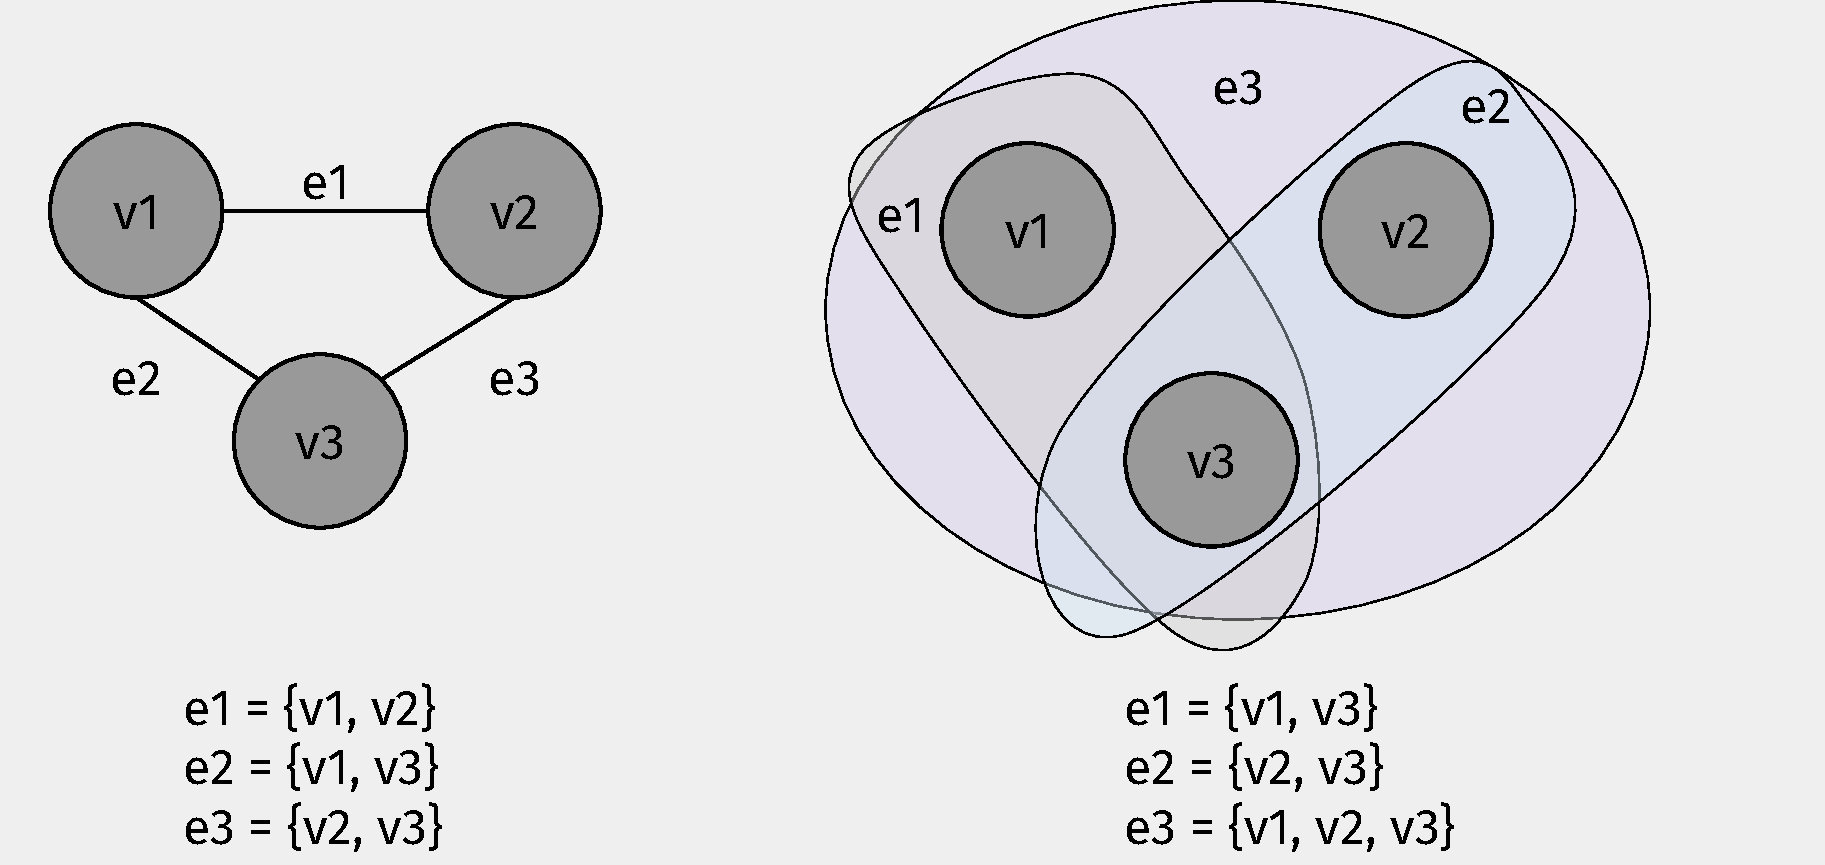
\includegraphics[width=0.7\linewidth]{images/Chapitre3/graph_vs_hgraph.pdf}
\caption{A graph (to the left) compared to a hypergraph (to the right). The edges of the hypergraph (hyperedges) may hold more than two nodes at once, relaxing the constraint of graphs' binary relations. A hypergraph can be seen as a set of $n$-ary sets: $E=\{\{v1,v3\},\{v2,v3\},\{v1,v2,v3\}\}$.}
\label{fig:graph_vs_hgraph}
\end{figure}


Building upon previous linguistic representations \cite{2007.Klapaftis.UoY,2011.Haishan.AHypergraphbased,2014.Tao.Qian.LexicalChainHypergraphWSI}, our model is indeed based on the use of a hypergraph.
% As stated before, hypergraphs have been employed in the literature to model complex systems. 
Its single most important difference with regular graphs, being able to relate more than two vertices at the same type, allows for a better characterization of interactions within a set of individual elements (in our case, words) \cite{heintz2014beyond}. Indeed, our hypergraph modelization initially integrates four types of relations between tokens: sentence co-occurrence, part-of-speech tags, words' constituents data and dependency relations in a single linguistic structure. These relationships were chosen because it is relatively easy to obtain them for high-resource languages. These features can be seen as building blocks for NLP models. Extracting deeper language features would implicate relying even more on general domain systems. In any case, our goal is to arrive to more complex annotations (e.g., named entities) from the selected features and relations. Indeed, as we discussed before, different types of contexts give us different types of similarities. Recall that a  smaller lexical window  gives us co-occurrence relations that approach functional relatedness, such as those found with syntactic contexts. That is why we decided to keep a lexical context at sentence level, so that it may complement the distributional semantic information provided by the dependency functions context as well as the phrase-constituency syntactic context. In short, we  aim to cover three levels of possible semantic relatedness via  three levels (in terms of the size of the neighborhood of a target word) of distributional co-occurrences 
%todo (see Figure \ref{})
: a short range with dependency functions, a medium range with phrase constituency membership, and a longer range with sentence lexical co-occurrences. The intuition is that when solving NLP tasks, having direct access to these three semantic spaces will help to determine a more appropriate meaning's relation between words. 

 
\paragraph{Construction}
In our case, the set of words in the corpus are the set of nodes  $V$, and the set of hyperedges  $E$ represent the relations between nodes according to different linguistic aspects.
%
We consider each word (i.e., each node) to exist in one of three types of hyperedges, two syntactic and one lexical co-occurrence contexts:
\begin{enumerate}
\item $\textsc{\textbf{NP}}$: noun phrase (NP)  constituents,
\item $\textsc{\textbf{DEP}}$: dependency relations. We consider all types of dependency functions between nouns and verbs,
\item  $\textsc{\textbf{SEN}}$: lexical context, in this case the window considered is the whole sentence
\end{enumerate} 

The part of speech information is stored implicitly with the constituent information. While these parameters are fixed in our implementation, they can easily be adapted to other configurations. For example, we may consider noun phrases and verb phrases as chunks, specific types of dependency functions, or different lexical window size.

To populate the hypergraph, given a token $v$, a noun phrase $p$, a sentence $s$, and a 
dependency function $dep(h, \cdot)$, with $h$ being the head of the relation, we consider the following rules:

\begin{itemize}
\item $v$ is incident (or belongs) to a hyperedge $e_j$ of type NP if  $v$ appears in the same noun phrase $p$.
\item The same condition is used with sentence hyperedges SEN: if  $v$ appears in a sentence $s$, it will be located in a hyperedge $e_j$ of type SEN. 
\item If $v$ participates in a dependency function $dep(h,v)$ as a dependent, it belongs to a hyperedge $e_j$ of type DEP.
\end{itemize}

Each hyperedge is labeled according to an identifier that allows the hypergraph to be populated while reading words from a corpus. For example, the hyperedges of the set $\textsc{\textbf{SEN}}=\{h_{S_1}, h_{S_2}, h_{S_3}\}$ are indeed hyperedges that represent sentences, identified by an index in this case. Hyperedges $h_{S_1}, h_{S_2}, h_{S_3}$ contain each a set of words. Additionally, the hypergraph can be represented as a $n \times m$ incidence $H$ matrix with entries $h(i,j) = N(v_i, e_j)$ where $N(v_i, e_j)$ is the number of times $v_i \in e_j$ occurs in the corpus. This frequency values can be later converted into other weighting schemes as seen in Chapter \ref{chap:backgnd}. Indeed, the incidence matrix allows us to pass from the hypergraph-based model of representation into the vector-space model.

\paragraph{Running Example}
We illustrate the process of creating a sample hypergraph model with the following example phrase: \textit{The report contains copies of the minutes of these meetings}.  We tokenize the phrase, keeping all the words, and we lemmatize and parse it to obtain both constituency and dependency trees. 

\subparagraph{Constituency Tree} The constituency tree of the example phrase is shown in Figure \ref{fig:tree_constits}. The sentence, as well as each noun phrase (\textit{NP}) node is identified by a number, these numbers serve as an unique identifier of the phrase chunk within the whole sentence. We can observe that this phrase is composed by five noun phrases and one verb phrase. Meanwhile, some \textit{NP} are formed by other kind of phrases, depending on the grammar production rule used to build each one of them. Furthermore, as is usual in this kind of structures, there is a one to one relation between the number of tokens in the sentence  and the number of leaves in the tree.

For clarity,  in our example we  only consider nouns and the first three noun phrases (from left to right), as well as the nominal subject (\textit{nsubj}) and direct object (\textit{dobj}) dependency relations. Thus, in total, as described below, we have three hyperedges of noun phrase type: $NP_1, NP_2$ and $NP_3$. Each of them corresponding to the noun phrases in the constituents tree.
 
\subparagraph{Dependency Tree}
The dependencies of the example phrase are shown in Figure \ref{fig:tree_deps_report} as a tree structure. The relations can also be seen as tuples in Table \ref{tab:depends_report} In these relations' examples, the head is the first token to appear  followed by the dependent word. Two hyperedges are found: 
$nsubj_{contains}$ and $dobj_{contains}$.
 \begin{figure}
 \centering
 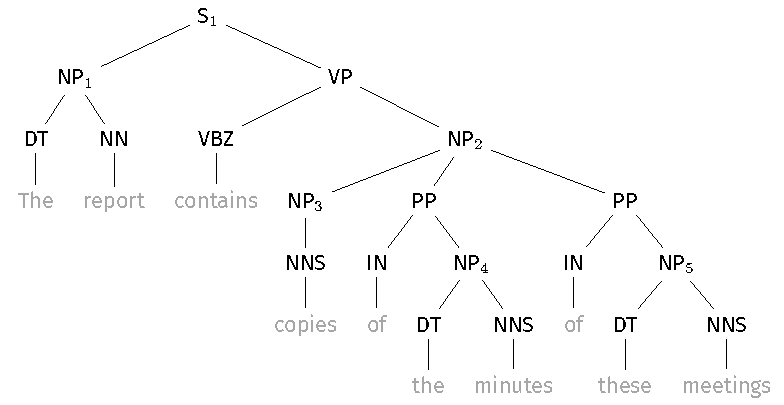
\includegraphics[width=0.7\linewidth]{images/Chapitre3/trees/tree_constits.pdf}
 \caption{Constituency-based tree of the phrase \textit{The report contains copies of the minutes of these meetings.}}
 \label{fig:tree_constits}
 \end{figure}
 
 %todo compare levels of semanticity in the three proposed models
 %
 
\begin{figure}[]
	\begin{minipage}{\textwidth}
		\begin{minipage}{.9\textwidth}
		\centering
		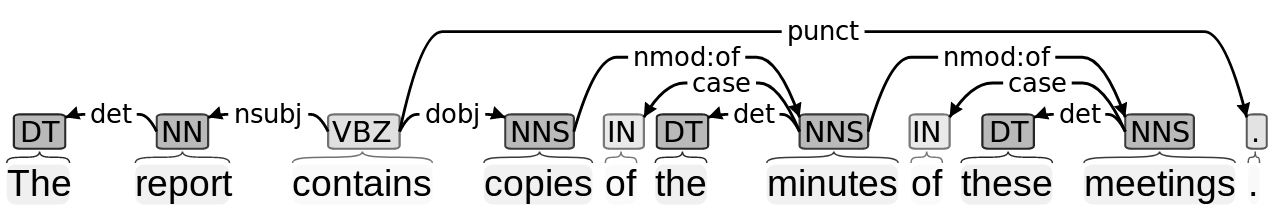
\includegraphics[width=0.9\linewidth]{images/Chapitre3/tree_deps_report.png}
		\captionof{figure}{Dependency-based tree of the example phrase.}
		\label{fig:tree_deps_report}
		\end{minipage} 
		\vspace{1cm}
		
		\begin{minipage}{.9\textwidth}
		\centering
		\begin{tabular}{@{}ll@{}}
%		 \toprule
		 \textbf{root}(root, contains)    & \textbf{det}(minutes, the)       \\
		 \textbf{det}(report, The)        & \textbf{nmod:of}(copies, minutes)   \\
		 \textbf{dobj}(contains, copies)  & \textbf{det}(meetings, these)    \\
		 \textbf{nmod:of}(minutes, meetings)       & \textbf{nmod}(minutes, meetings) \\
		 \textbf{nsubj}(contains, report) &
		 \end{tabular}
		 \captionof{table}{Dependency relations of the example phrase.}
		 \label{tab:depends_report}
		\end{minipage} 
	\end{minipage}	
\end{figure}


 
\subparagraph{Hyperedges Found}
From both syntactic parses and the phrase itself we build a hypergraph representation as stated before.  We show below the hyperedges sets found for each type,  (NP, SEN, and DEP), and their members. Each hyperedge  is labeled  with a unique identifier:
%todo imagen con el hypergrafo completo would be nice
\begin{itemize}
\item $\textsc{\textbf{NP}}=\{NP_1, NP_2, NP_3\}$
	\begin{itemize}
		\item $NP_1=\{report\}$	
		\item $NP_2=\{copies,\,minutes,\,meetings\}$
		\item $NP_3=\{minutes\}$
	\end{itemize}
\item $\textsc{\textbf{SEN}}=\{S_1\}$
	\begin{itemize}
		\item $S_1=\{report,\,contains,\,copies,\,minutes,\,meetings\}$	
	\end{itemize}
\item $\textsc{\textbf{DEP}}=\{nsubj_{contains},\,dobj_{contains}\}$
	\begin{itemize}
		\item $nsubj_{contains}=\{report\}$	
		\item $dobj_{contains}=\{copies\}$	
	\end{itemize}

\end{itemize}

\subparagraph{Incidence Matrix}\index{Incidence Matrix}We can represent these hyperedges as an incidence matrix, illustrated in Figure \ref{fig:incidence_report}.  
Looking at the table, we can   infer that the word \textit{copies} appears  in two hyperedges of type NP: first in \textit{NP$_2$}, which is built from a noun phrase  and two prepositional phrases (\textit{PP}). Secondly, we see that it is part of \textit{NP$_3$}, which  indicates a plural noun (\textit{NNS}).
Regarding the syntactic dependency hyperedges, the word \textit{copies} appear in the \textit{dobj} \textit{contains} column which indicates that \textit{copies} was the direct object of the verb \textit{contains}. Concerning the sentence hyperedges, we see that the token \textit{copies} appeared in the same sentence S$_1$ as the other four noun words.

\begin{figure}
\centering
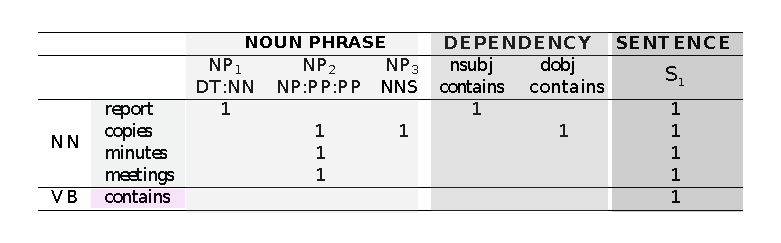
\includegraphics[width=\linewidth]{images/Chapitre3/incidence_mat.pdf}
\caption{Incidence matrix of the example phrase hypergraph modelization.}
\label{fig:incidence_report}
%todo change font to fira of this pic!
\end{figure}


%\paragraph{Discussion}
With the short example presented we show the intuitive way in which we identify three different kinds of relations: lexical co-occurrence (at sentence level), dependency co-occurrence, and noun phrase co-occurrence. Looking at the incidence matrix we see the three levels of semantic relatedness we aim to represent with the three different types of context: sentence, dependency, and noun phrase level. At the same time, there is a structure within the hypergraphs. Groups of words are found to be together either directly or by means of paths traced by other nodes. 

On the other hand, we realize that the incidence matrix is relatively sparse and this it will inevitably increase as more text is included in the hypergraph. Sparsity, as we saw previously, affects the performance of knowledge discovery techniques applied to NLP tasks. 

Just as the literature approaches covered before, we aim to solve semantic tasks by using the proposed linguistic resource and its relations. Yet, unlike those approaches we have three contexts and thus three levels of semantic relatedness, coupled to the $n$-ary relations from the hypergraph structure. Nonetheless, our model also suffers from data sparsity. We will show how to deal with this issue in the following section. The general idea is that by combining features from the different contexts we can alleviate the problem as similarities not seen in a context may complement the features from another context. The set of approaches that perform this combination are known as multimedia fusion techniques.
% We can thus build systems that allow us to interpret a word from different perspectives according to said relations.




                                                                                            
\subsection{Representation Enrichment with Fusion Techniques}\label{sec:fusion}
 

\begin{table}[]
\centering
\begin{tabular}{ll}
\textbf{Notation}               & \textbf{Definition}                                                          \\
$A,B$                  & Single modality representation matrices                                            \\
$\mlex$                & Lexical representation matrix                                       \\
$\msyn$                & Syntactic representation matrix                                     \\
$\mstd$                & Standard features representation matrix                              \\
$\slex$                & Lexical similarity matrix                                           \\
$\ssyn$                & Syntactic similarity matrix                                         \\
$\sstd$                & Standard similarity matrix                                          \\
$E_\alpha(A,B)$        & Early fusion representation space from matrices A and B             \\
\textbf{hstack}                 & Function that joins together two matrices column-wise               \\
$\alpha$               & Early fusion parameter that weighs input matrices                   \\
$L_\beta(A,B)$         & Late fusion representation spaces from matrices A and B             \\
$\beta$                & Late fusion parameter that weighs input matrices                    \\
$X_\gamma(A,B)$        & Cross fusion representation from matrices A and B                   \\
$\mathbf{K}(A,\gamma)$ & Operator yielding the top $\gamma$ neighbors of similarity matrix A \\
$\gamma$ 			   & Cross fusion parameter that determines the number of similar neighborhoods to take with the $\mathbf{K}$ function \\
$X_F$                  & Cross Feature fusion                                                \\
$X_S$                  & Cross Similarity fusion                                             \\
$X_FEF$                & Cross Feature Early Fusion                                          \\
$X_FX_SF$              & Cross Feature Cross Similarity Fusion                               \\
$EX_FF$                & Early Cross Feature Fusion                                          \\
$LX_FF$                & Late Cross Feature Fusion                                           \\
$ELX_FF$               & Early Late Cross Feature Fusion                                     \\
$EEELX_FLX_F$           & Triple Early Double Late Cross Feature Fusion                      
\end{tabular}
\caption{Fusion related notations and definitions}
\label{tab:fusion_notation}

\end{table}

%\printnomenclature

%We first describe below multimedia (or multimodal) fusion techniques  as well as relevant use cases where they have been employed. 
%Then, we focus exclusively on fusion techniques applied to NLP tasks, which is the general domain of the two tasks (NER and WSI/WSD) we focus on.                   

The second part of our proposed method deals with the fusion of textual features. For convenience, we start by introducing in Table \ref{tab:fusion_notation} the notations we use in the description of our fusion approaches. Specifically, by using fusion operators, we combine the features that describe terms into a single representation space. This new space aims to address two issues that arise while working with textual data: effectively using information coming from different linguistic levels (e.g., lexical, syntactic, semantic) while alleviating the sparsity typical of textual representations.

Multimodal fusion \index{Multimodal fusion} entails set of popular techniques used in multimedia analysis tasks. These methods integrate multiple media features, the affinities among these attributes or the decisions obtained from systems trained with said features, to obtain rich insights about the data being used and thus to solve a given analysis  task \cite{AtreyHEK10}. We note that these techniques come at the price of augmenting the complexity of a given system by increasing or reducing the sparsity of a given feature matrix.


In the multimodal fusion literature we can discern two main common types of techniques: early fusion and late fusion. A third and fourth type of fusion methods, cross-media fusion and hybrid fusion are also employed in multimedia analysis tasks. 

These four fusion operators naturally address the issue of dealing with heterogeneous data as they all mix one way or another the feature columns from each of two representations. Regarding alleviating sparsity, the intuition is that by combining matrices either by summing or element-wise multiplying them, the resulting matrix will have a denser structure. For example, by summing two matrices with the same shape, such as two term-term similarity matrices, we  obtain a resulting matrix that contains the similarities of both feature spaces. In the same sense, when multiplying two matrices we combine them while also obtaining a denser output matrix. Nonetheless, both sum and multiplication result depends evidently on the nature of the matrices employed. Two of the fusion techniques mentioned above, late fusion and cross-media fusion use sum and multiplication as they  main matrix operator. What is more, both of them contemplate the use of similarity matrices as at least one of their inputs. Being similarity matrices, they tend to be dense and thus the resulting sum or product will be more dense than the original sparse representation, while complementing and enriching the space with other types of information. We present an example of this intuition in the following section.


We describe the four of them in the following paragraphs. The notation used is first introduced as follows. The fusion functions are binary, they all take two inputs, parameters $A$ and parameter $B$ which define arbitrary single-modality matrices. For example, both matrices $A$ and $B$ may represent a lexical $M^{L}$, syntactical based $M^{S}$, or other type representation spaces $M^{T}$. On the other hand, they may also describe their  respective similarity (square) matrices, $S^{L}$ and  $S^{S}$. In a broader sense, matrices $A$ and $B$ may represent any pair of valid\footnote{Valid in terms of having compatible shapes while computing a matrix sum or multiplication.} term-feature matrices.



\paragraph{Early Fusion} \index{Early Fusion}
This technique is the most widely used fusion method. The principle is simple: we take both modal features and concatenate them into a single representation matrix. More formally, we consider two matrices  that represent different modality features each  over the same set of individuals. To perform early fusion we concatenate them column-wise, such that we form a new matrix having the same number of lines but increasing the number of columns to the sum of the number of columns of both matrices. The matrices may also be weighted as to control the influence of each modality.

Such trivial fusion  is shown in Figure \ref{fig:ef_diag}. In this example, two  matrices are used, $\mlex$ and $\msyn$. Each one represents a different feature space. They both have the same number of rows $n$, they have $m$ and $p$ columns, respectively. After an early fusion operation, the final matrix  has $m+p$ features. Formally, the early fusion function is defined as:
\begin{equation}
E(A,B) = \mathbf{hstack}(A , B)
\end{equation}
As stated before, the matrices $A$ and $B$ are combined together via a concatenation function $\mathbf{hstack}$ which joins both of them column-wise. In order for this operator to work, both matrices must have the same $n$ number of rows.

During the concatenation, we may also apply a weight to matrices $A$ and $B$ such as: 
\begin{equation}
E_\alpha(A,B) = \mathbf{hstack}(\alpha\cdot A , (1-\alpha)\cdot B)
\end{equation}
Indeed, this weighted early fusion  represents the same operation as before with an extra parameter: $\alpha$, which controls the relative importance of each matrix. In the following, we refer to both operations simply as early fusion. When $\alpha$ is determined (and indicated as a subscript), we refer to weighted early fusion. Otherwise, there is no weighting scheme applied to the operation.

The main advantage of early fusion is that a single unique model is fitted while leveraging the correlations among the concatenated features. The method is also easy to integrate into an analysis system. The main drawback is that we increase the representation space and may make it harder to fit models over it.

\begin{figure}
\centering
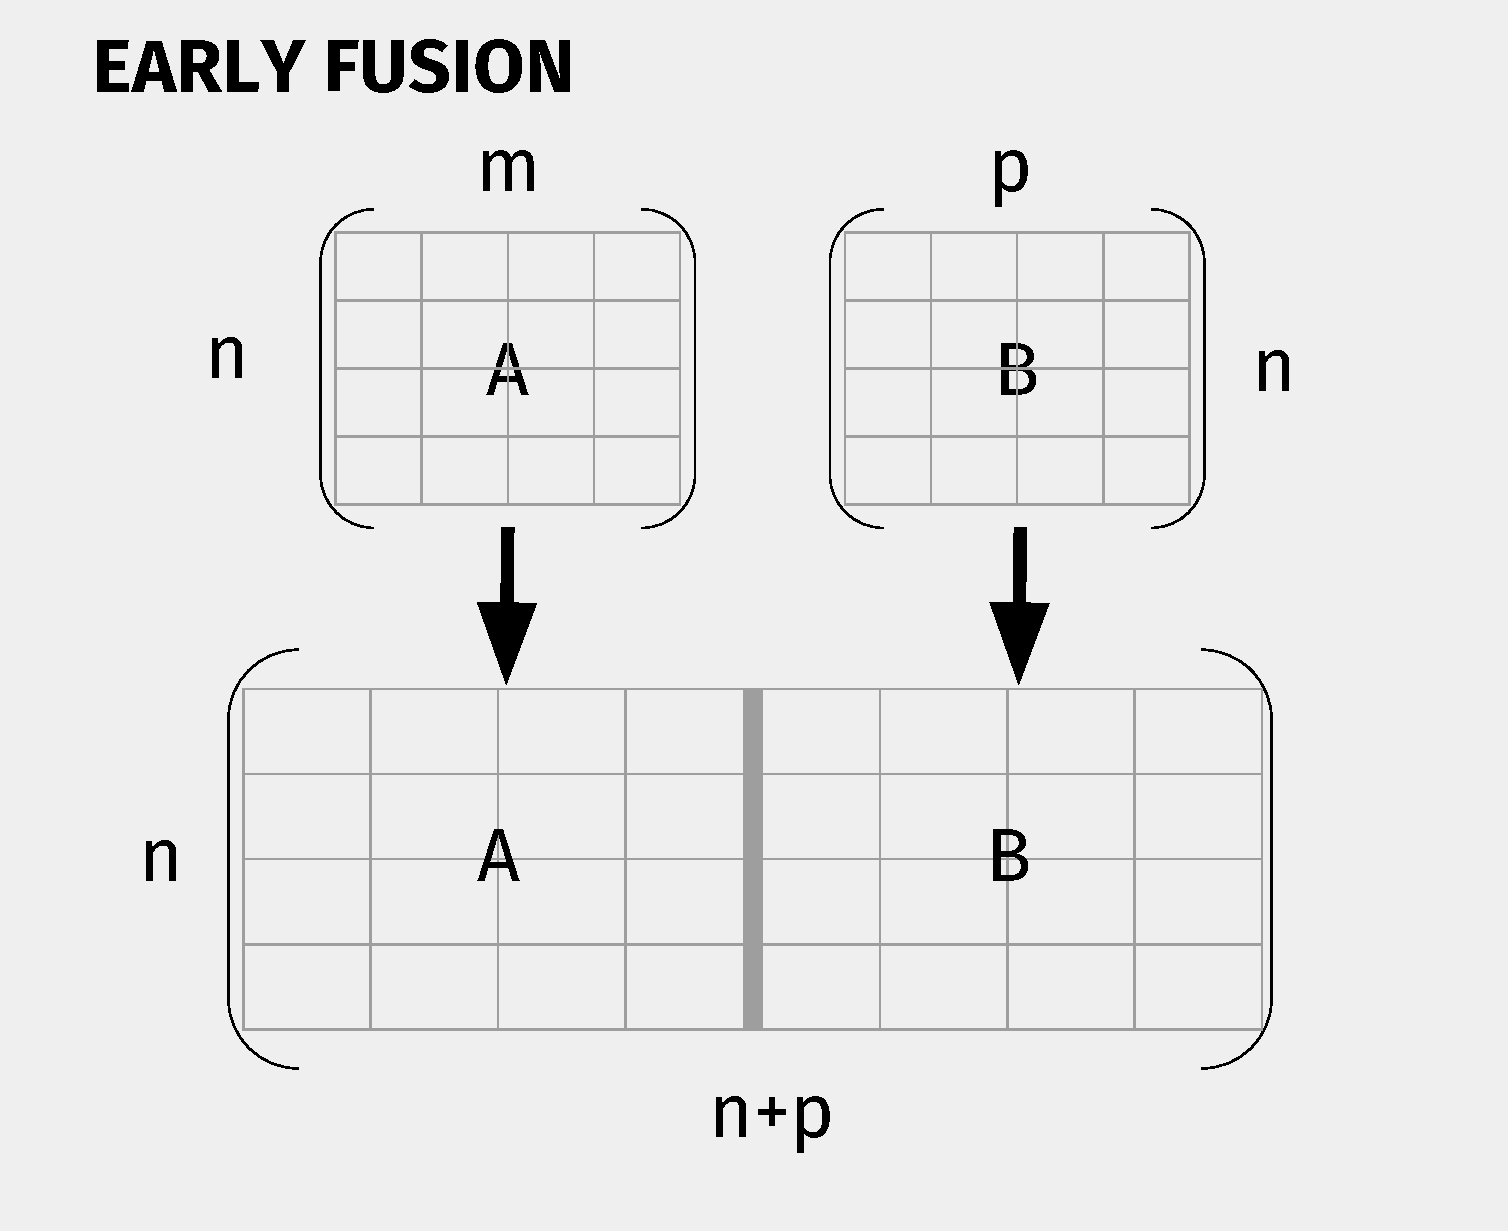
\includegraphics[width=0.7\linewidth]{images/Chapitre3/ef_diag.pdf}
\caption{Early Fusion of feature matrices $A$ and $B$. The result is the concatenation of both matrices.}
\label{fig:ef_diag}
\end{figure}


%

%   of shape $(n, m + p)$. Following the literature notation of [vulic], the early fusion representation matrix EF is defined as:
%\begin{equation}
%EF = \alpha \times X_1 || (1 - \alpha) \times X_2
%\end{equation}

%where $||$ represents the column-wise concatenation operation and ? is the parameter that determines the contribution of each modality. 
%
%Early fusion has been employed in several multimodal tasks. For example, [?]. 
\paragraph{Late Fusion}\index{Late Fusion}
In contrast to early fusion, in late fusion the combination of multimodal features are generally performed at the decision level, i.e., using the output of independent knowledge discovery models trained  each with a unique set of features \cite{ClinchantAC11}. In this setting,  decisions produced by each model are combined into a single final result set. The diagram in Figure \ref{fig:lf1} shows this combination of matrices $A$ and $B$.
%
The methods used to combine preliminary decisions usually involve one of two types: rule-based (where modalities are combined according to domain-specific knowledge) or linear fusion (e.g., weighting and then adding or multiplying both matrices together). This particular type of fusion is very close to machine learning  ensemble methods.
%

Indeed, late fusion combines both modalities in the same semantic space. In that sense,  we may also combine modalities via an affinity representation instead of final decision sets. In other words, we may combine two modalities  by means of their respective similarity matrices. In this case, a  representation is  obtained by adding  two similarity matrices, as in Figure \ref{fig:lf2}. In the figure, we use the equal-sized matrices $S^L$ and $S^S$, which in this case are the similarity matrices of matrices $\mlex$ and $\msyn$. Both matrices are then summed to produce a single $n \times n$ weighted matrix (determined by a parameter $\beta$). 
%

More formally, we define the late fusion function as:
\begin{equation} \label{eq:late-fusion}
L_\beta(A,B) = \beta \cdot A + (1 - \beta)\cdot B
\end{equation}

In this function, the extra parameter $\beta$ affects the influence of matrix $A$,  and consequently also the relevance of matrix $B$. As we are summing two matrices, for this operator both $A$ and $B$ must be of the same size.


The advantages of late fusion include the combination of features at the same level of representation (either the fusion of decisions or similarity matrices). Also, given that independent models are trained separately, we can choose which algorithm is more adequate for each type of features. 



\begin{figure}
	\centering
	\begin{subfigure}[t]{.5\textwidth}
	\centering
	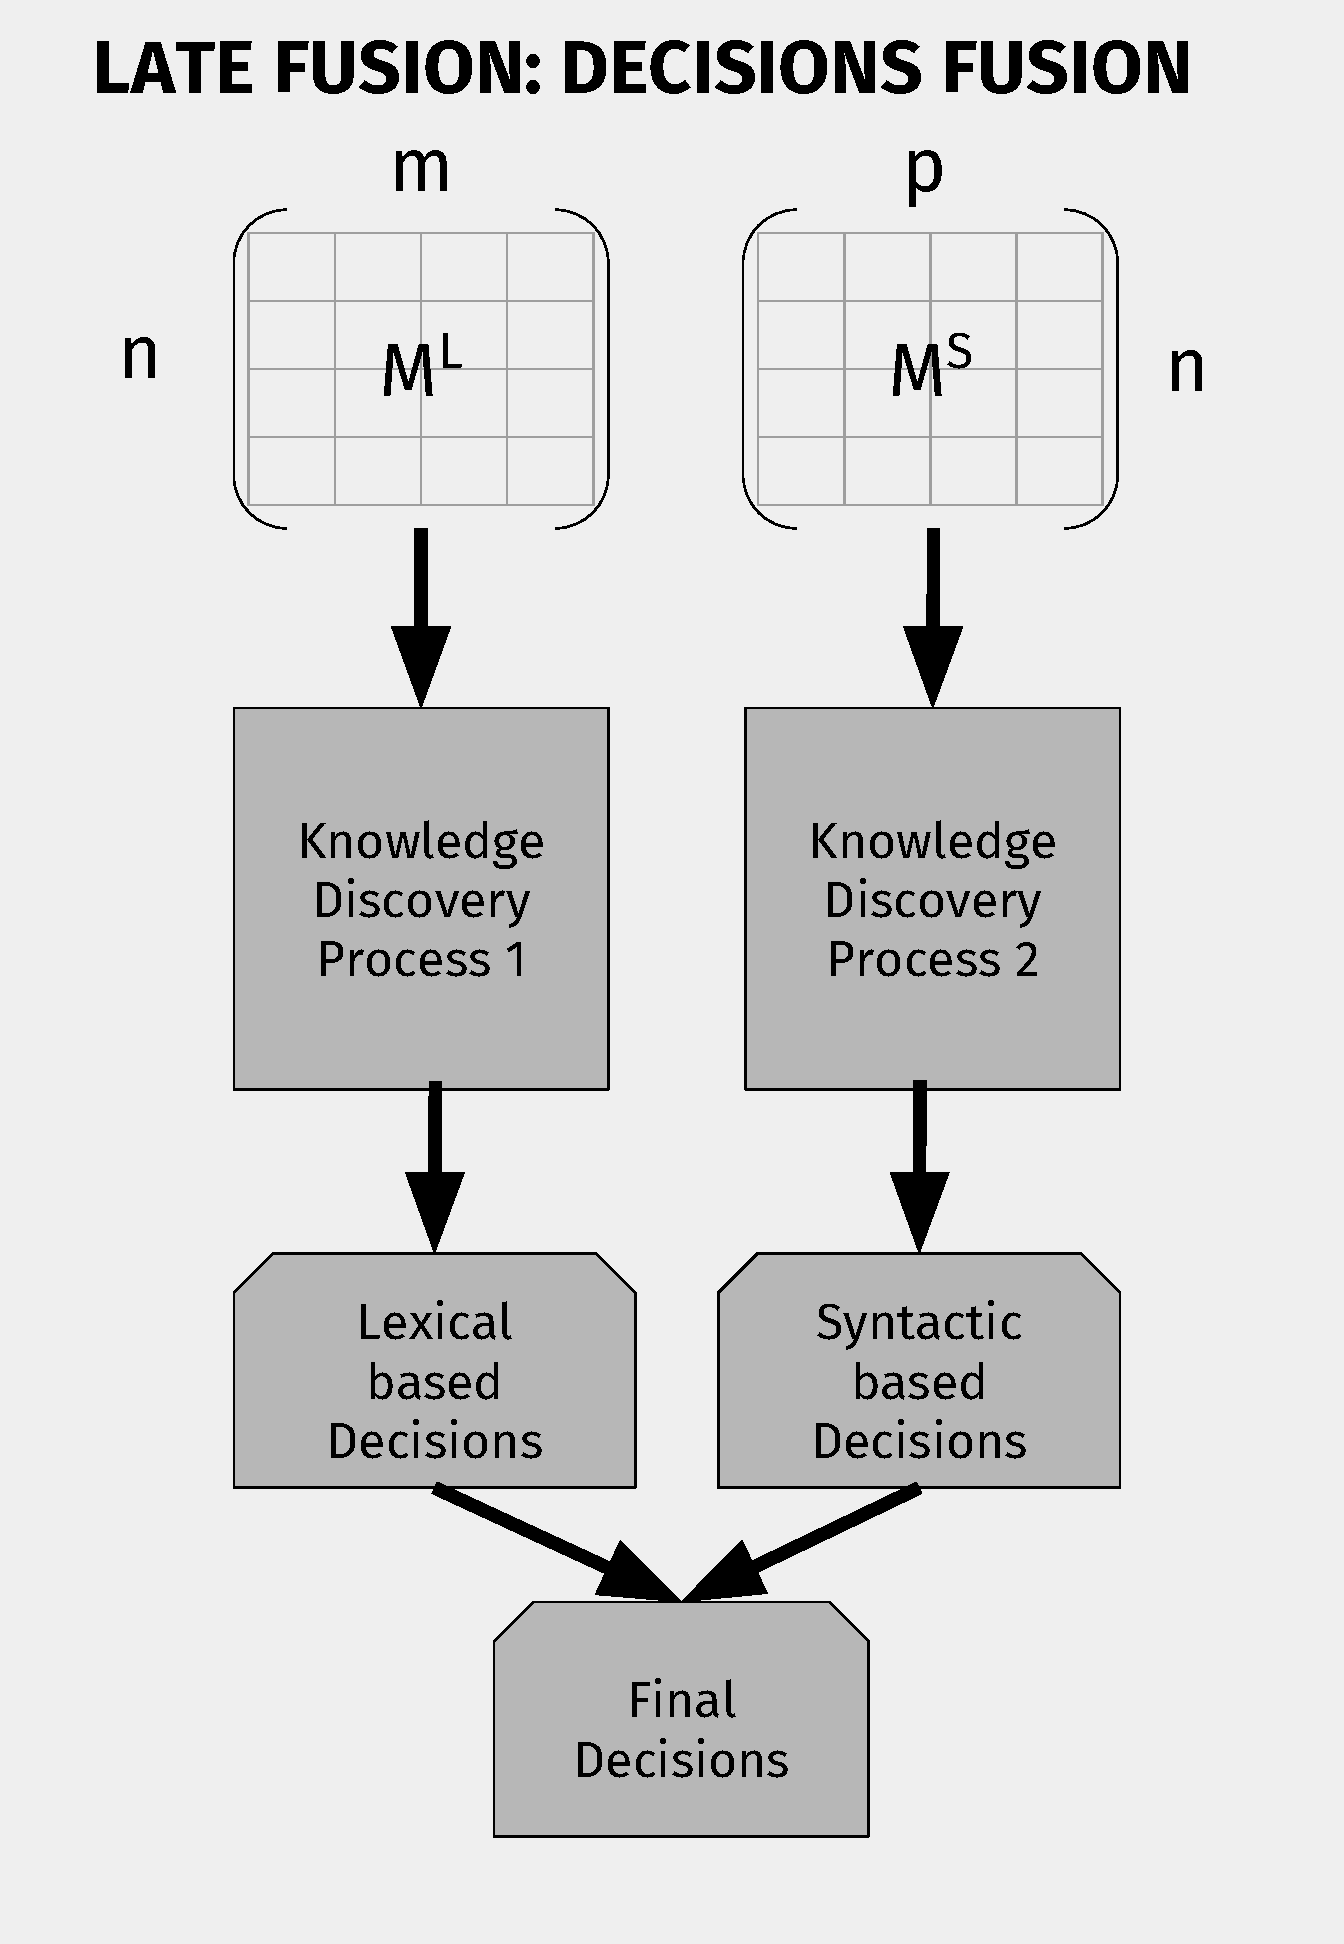
\includegraphics[width=0.9\linewidth]{images/Chapitre3/lf1_diag.pdf}
	\caption{Fusion of decisions.}
	\label{fig:lf1}
	\end{subfigure}% 
	\begin{subfigure}[t]{.5\textwidth}
	\centering
	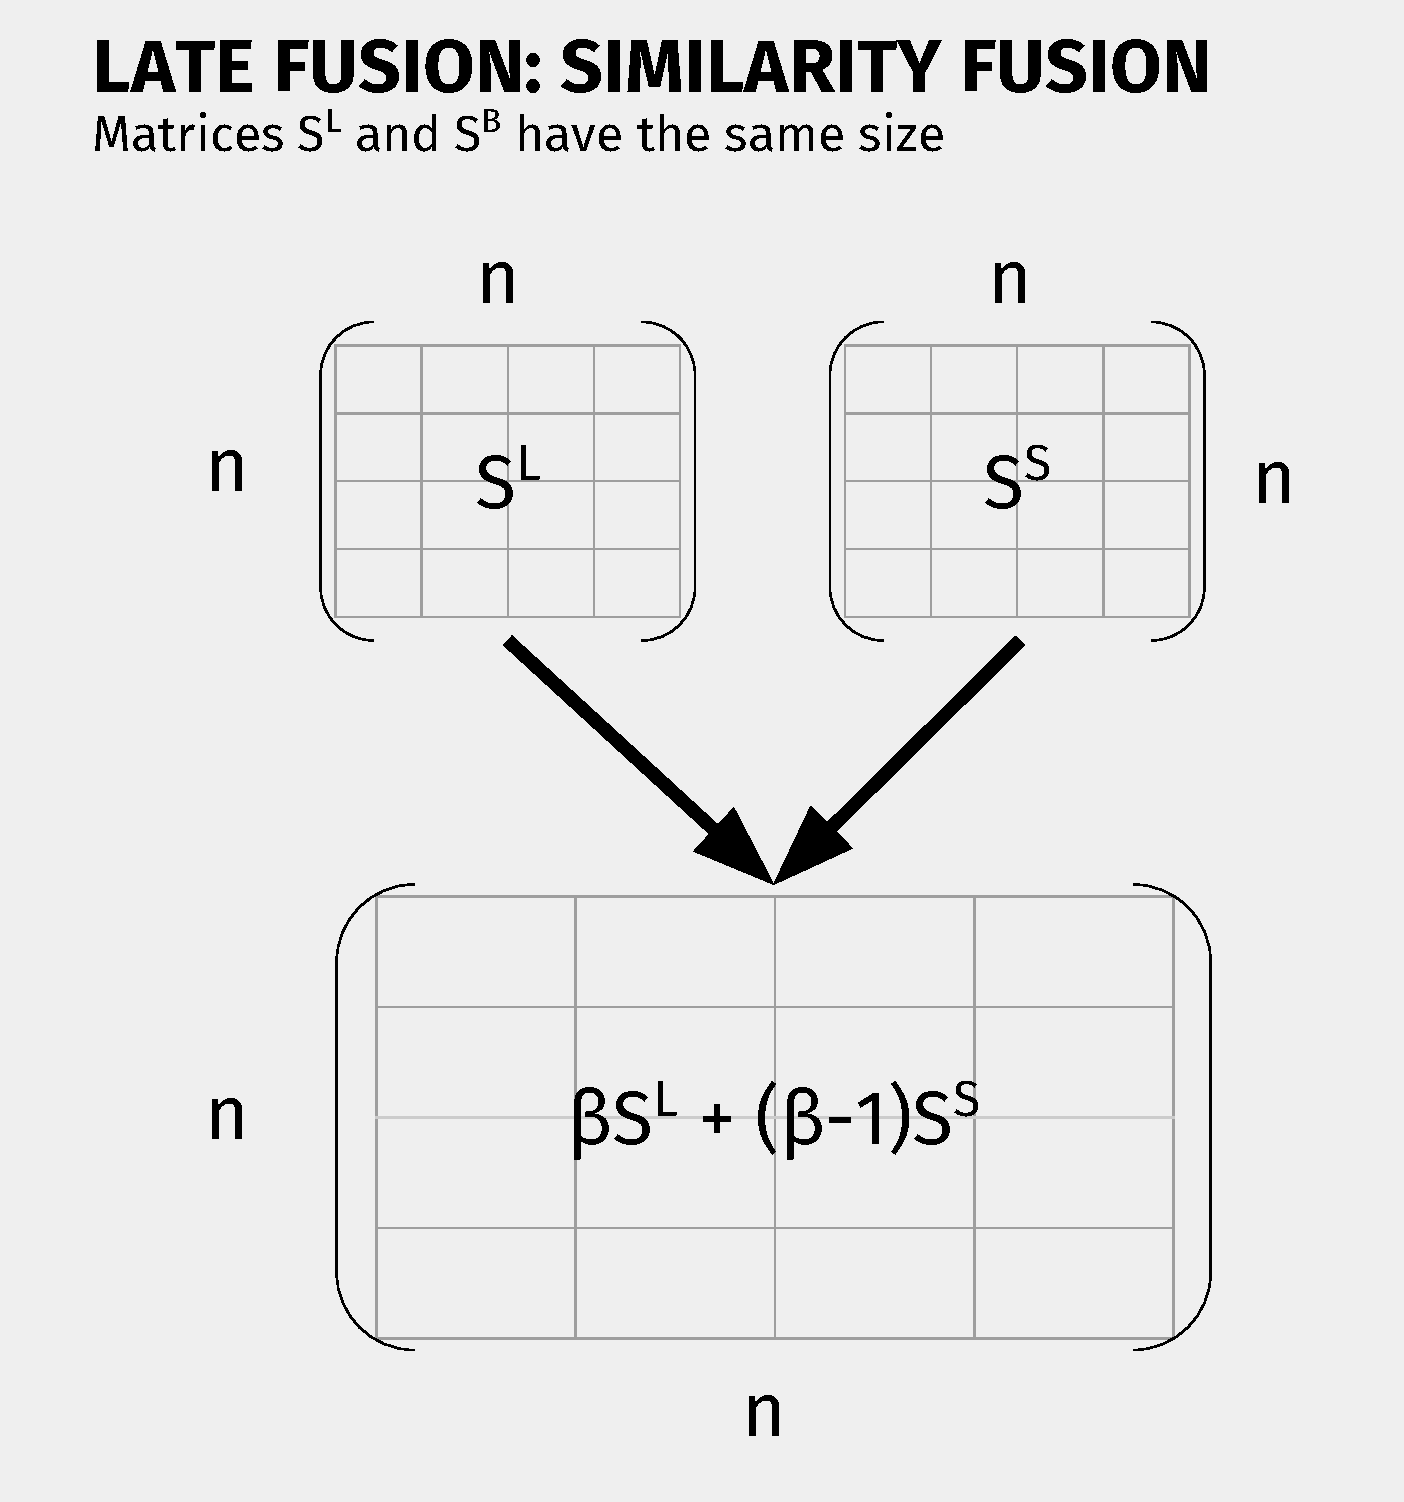
\includegraphics[width=0.9\linewidth]{images/Chapitre3/lf2_diag.pdf}
	\caption{Fusion of similarity matrices.}
	\label{fig:lf2}	
	\end{subfigure}
	\caption{Late fusion possibilities. To the left, fusion of knowledge discovery models' decisions. To the right, fusion of similarity matrices.}
	\label{fig:lf_diag}
\end{figure}




%For example, in information retrieval (Ah-Pine et al., 2015), lexicon learning (Vulic et al., 2016), coreference resolution (Eisenstein and Davis, 2007); different types of representations (different modalities) can be combined in order to take advantage of the complementarity existing among them
\paragraph{Cross-media  Fusion}{Cross Fusion}
%
A third type of fusion technique, cross-media  fusion (or simply cross fusion),   introduced in \cite{ClinchantAC11,Ah-PineCC15}, is defined and employed to propagate a single similarity matrix into a second similarity matrix. In their paper, the authors propagated information from textual media towards visual media. In our case, we transfer information among textual features. For example, to perform a cross fusion between lexical and syntactical features, we perform the following steps: 
\begin{enumerate}
\item Compute the corresponding similarity matrices for each type of features.
\item Keep only the nearest neighbors for each word within the lexical similarity matrix while assigning zero to the rest.  These selected neighbors are to be used as lexical representatives to enrich the syntactical similarities.
\item Linearly combine both similarity matrices  via a matrix product.
\end{enumerate}  

\begin{figure}
\centering
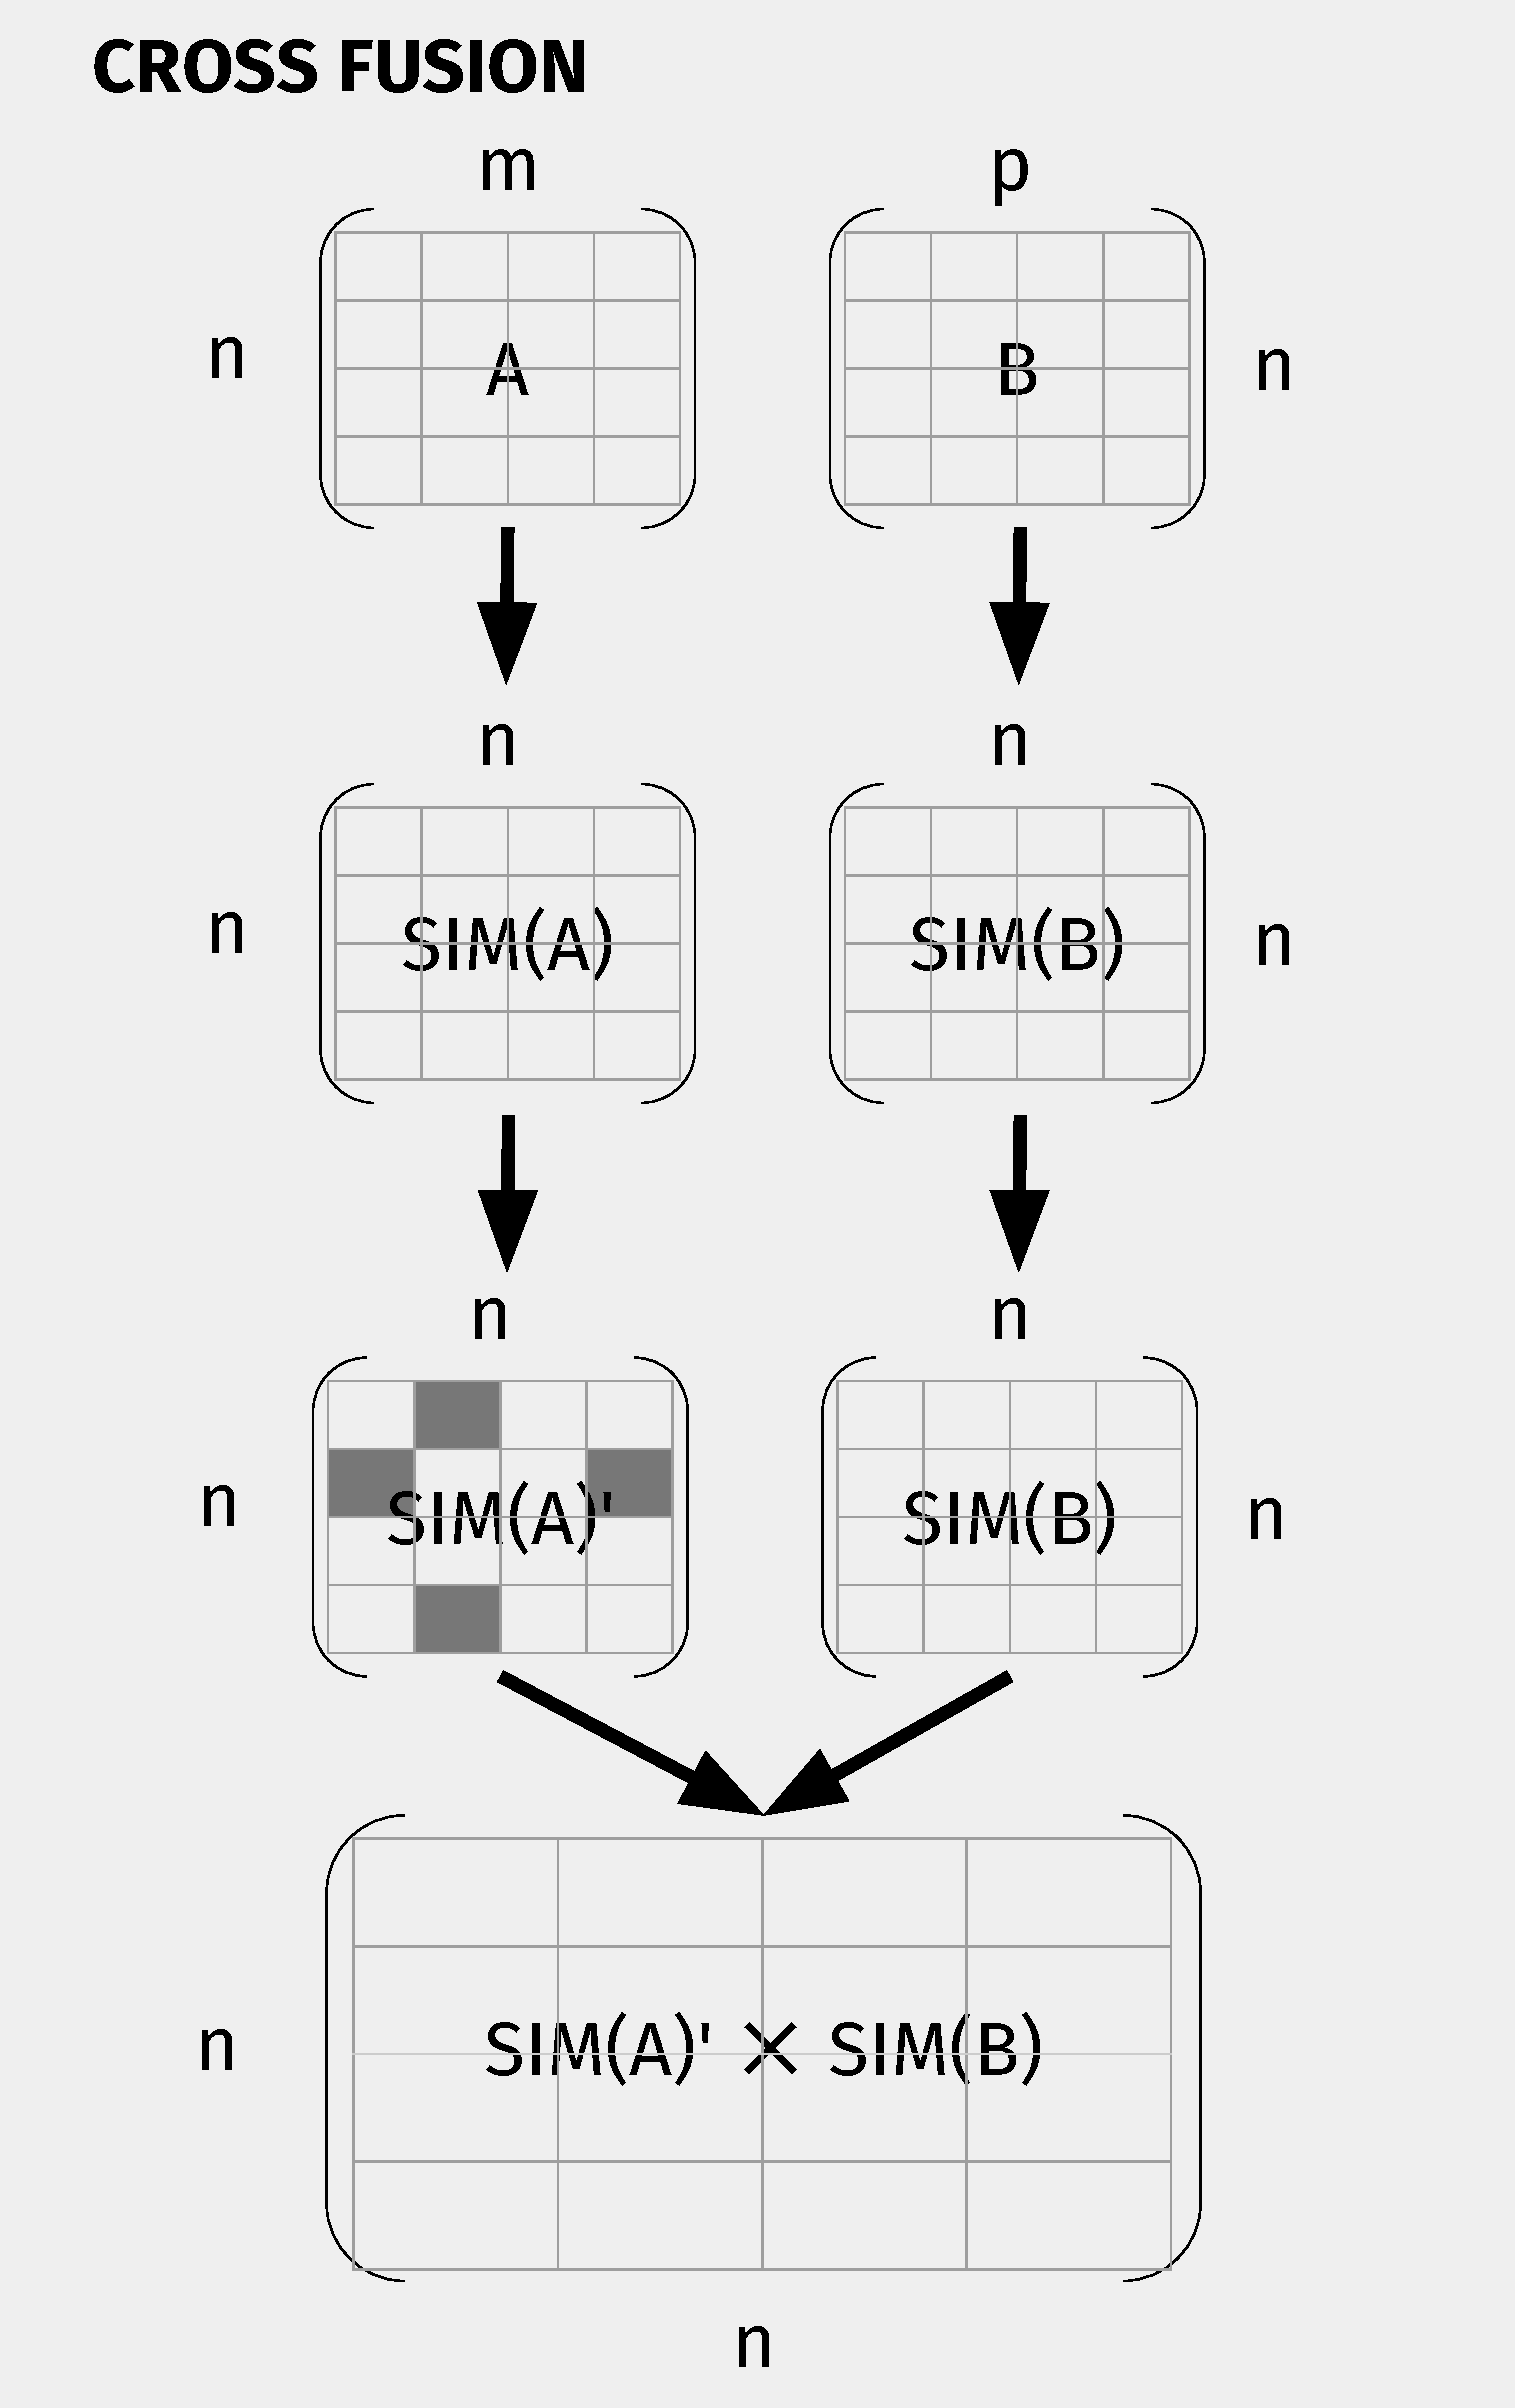
\includegraphics[width=0.6\linewidth]{images/Chapitre3/xf_diag.pdf}
\caption{Cross fusion for matrices $A$ and $B$. Similarities are computed, the best similarities are selected for $A$ and finally a product is calculated between the similarities of $B$ and the top similarities of $A$.}
\label{fig:xf_diag}
\end{figure}

Figure \ref{fig:xf_diag} shows this cross fusion example, between matrices $\mlex$ and $\msyn$. First, their corresponding similarity matrices $\slex$ and $\ssyn$ are first obtained. Secondly, a  top-nearest neighbors operation is applied, $\mathbf{K}(\slex, \gamma)$, yielding a matrix which contains only the most representative similarities, determined by the parameter $\gamma$. Finally, the cross fusion representation is obtained by computing the product $\mathbf{K}(\slex, \gamma) \times \ssyn$.

Formally, we define the cross fusion function as:
\begin{equation}\label{eq:xfusion}
X_{\gamma}(A,B) = \mathbf{K}(A,\gamma) \times B
\end{equation}

In this case, the $\mathbf{K}(\cdot)$ function takes the top-$\gamma$ closest words (columns) to each word (lines) while the rest of the values are set to zero. As noted before, matrices $A$ and $B$ may be two similarity matrices. While $A$ is always required to be a square filtered similarity matrix, $B$ may be also a plain term-feature matrix, as we describe in the following paragraphs.
The sole requirement is that the  number of columns of the result of the operation $\mathbf{K}(\cdot)$ should be equal to the number of rows of $B$.

Cross fusion aims to bridge the semantic gap between two modalities by using the most similar neighbors as proxies to transfer valuable information  from one modality onto another one. Usually, the result of a cross fusion is combined with the previous techniques, early and late fusion. In this work we perform  experiment in that sense.

\paragraph{Hybrid Fusion}\index{Hybrid Fusion}
We may leverage the advantages of the previous three types of fusion techniques by combining them once more in a hybrid setting. As described in \cite{AtreyHEK10,yu2014informedia}, the main idea is to simultaneously combine features at the feature level, i.e., early fusion, and at the same semantic space or decision level. Nonetheless, they define a specific type of hybrid fusion. In this chapter, we adopt a looser definition of hybrid fusion. That is, we perform a hybrid combination of features by leveraging the aggregation of the fusion strategies described before. 

Having said that, here we distinguish three levels of hybrid fusion (aside from the use of single features, or SF henceforth, independently) that we employ in our experiments during the Chapter \ref{chap:wsd}. 

 \begin{enumerate}
\item \textbf{First Degree Fusion (1F)}\index{{First Degree Fusion (1F)}}: we  consider the  three elementary fusion techniques described before (early fusion, late fusion, cross fusion) by themselves.  This level of fusion serve as the baseline we set to surpass in order to show the efficacy of the representation feature space found through fusion techniques.
As an example, we may obtain a first degree representation matrix by performing an early fusion between the lexical matrix and the syntactical features matrix: $E(M^{L}, M^{S})$. 

We note that we distinguish two types of cross fusion operators: \textbf{Cross Feature Fusion}\index{Cross Feature Fusion} ($X_F$) and \textbf{Cross Similarity Fusion}\index{Cross Similarity Fusion} ($X_S$). The former combines a similarity matrix with a feature matrix, e.g., $X_F(\slex, \msyn)$. The latter joins a similarity matrix with another similarity matrix, for example $X_S(\ssyn, \slex)$. %Indeed, $X_S$ has the same configuration as the cross fusion presented before. We rename it to distinguish against the $X_F$ configuration. 
The intuition behind cross feature fusion $X_F$ is that the rich information from the first input matrix can be transferred directly to a representation without the need of obtaining its similarity matrix beforehand. We denote them \textit{feature} and \textit{similarity} to refer to the fact that the first one uses simply a feature matrix and the second requires some knowledge from the data, in this case the similarity between terms.

\item \textbf{Second Degree Fusion (2F)}\index{Second Degree Fusion (2F)}: in this level we  begin with the recombination of the outputs of the previous two levels. Namely, this procedure  yields a combination of "second-degree" among fusion methods. Indeed, we introduce four types of second degree fusions employed in the following list. Each one is illustrated with an example:


\begin{enumerate}

\item \textbf{Cross Feature Early Fusion}\index{Cross Feature Early Fusion} ($X_FEF$): consists on the cross feature fusion ($X_F$) of two inputs, a similarity matrix, and the output of an early fusion. For example the operation $X_F(\sstd, E(\mlex, \msyn))$ implies the $X_F$ of the similarity matrix $\sstd$ with the early fusion of matrices $\mlex$ and $\msyn$.

% %
\item \textbf{Cross Feature Cross Similarity Fusion}\index{Cross Feature Cross Similarity Fusion} ($X_FX_SF$): entails the cross feature fusion ($X_F$) of two elements, the output of a cross similarity fusion ($X_S$), and a term-feature matrix. For example, the operation $X_F(X_S(\sstd, \ssyn), \mstd)$ is the cross feature fusion ($X_F$) of a cross similarity fusion ($X_S$), the late having similarity matrices $\sstd$ and $\ssyn$ as inputs, and a standard features matrix $\mstd$.

%
\item \textbf{Early Cross Feature Fusion}{Early Cross Feature Fusion} ($EX_FF$):  this operation consists on the early fusion of a feature matrix with the output of a cross similarity fusion. As an example, the operation $E(\mstd,X_F(\slex, \mstd))$ computes the early fusion of matrix $\mstd$ with the result of a $X_F$ with $\slex$ and $\mstd$ as operands. 
%

\item \textbf{Late Cross Feature Fusion}\index{Late Cross Feature Fusion} ($LX_FF$): this fusion implies the late fusion of a feature matrix with the output of a cross feature fusion. For example, the fusion $L(\mstd, X_F(\sstd, \mstd))$ describes a late fusion between the feature matrix $\mstd$ and the cross feature fusion among $\sstd$ and $\mstd$.
\end{enumerate}

% A second-degree fusion would be an early fusion of the lexical feature matrix with a cross fusion, expressed as $E(M^{L}, \allowbreak X(S^{T}, M^{T}))$.   
\item \textbf{Higher-Degree Fusion (HF)}\index{Higher-Degree Fusion (HF)}: in this last level we follow a similar approach to the previous level by combining the output of the second-degree fusion level multiple times (that is, more than two times) with other second-degree fusion outputs. In this level we test the following two fusion operations:
\begin{enumerate}
\item \textbf{Early Late Cross Feature Fusion}\index{Early Late Cross Feature Fusion} ($ELX_FF$): As an example for this fusion, the operation $E(\mstd, \allowbreak L(\msyn, X_F(\sstd, \mstd)))$ implies the combination of three fusion operations. From left to right, first we compute the early fusion (first operation) of  matrix $\mstd$, with the result of a late fusion (second operation) between feature matrix $\msyn$ and the result of a cross feature fusion, itself having as input matrices $\sstd$ and $\mstd$. Indeed, we perform three operations, an early fusion, a late fusion and a cross feature fusion, thus the name Early Late cross feature fusion of this operator.
\item \textbf{Triple Early Double Late Cross Feature Fusion\footnote{We adopted the \textit{double} and \textit{triple} notation to lighten the explicit name of this fusion operation: Early Early Early Late Cross Feature Late Cross Feature Fusion}}
\index{Triple Early Double Late Cross Feature Fusion}
%Early Early Early Late Cross Feature Late Cross Feature Fusion
 ($EEELX_FLX_F$): although it seems complex, this fusion scheme merely consists on the early fusion of the last two operators: $LX_FF$ and $ELX_FF$, with another feature matrix. As an example, the operator  $E(\mlex, E(E(\mstd,  L(\mstd, X_F(\sstd, \mstd))),\allowbreak L(\mlex, X_F(\ssyn, \mlex))))$ entails the early fusion of matrix $\mlex$ with the result of the early fusion of $ELX_FF$ with $LX_FF$.
\end{enumerate}

	
%As an example, the equation $E(L(M^{T}, \allowbreak X(S^{T}, M^{T})),  L(M^{L}, X(S^{S}, M^{L})))$  \allowbreak denotes the early fusion between two operations: (1) a late fusion between a lexical-features matrix and a cross fusion, and (2),  another late fusion consisting of a standard-features matrix (this matrix is detailed below)  and a cross fusion. In general, we determine a n-degree fusion empirically. That is to say, we look at the performance of second-degree fusions and try to improve the performance of the systems by recombining the fusion outputs via a n-degree combination. This process is in fact applied during the second-degree fusions also. 
	\end{enumerate}   


%\paragraph{Discussion}             
The fusion operators presented (early, late, and cross fusion) are simple and straight-forward. In total, there are three parameters to control: $\alpha$ and $\beta$ in early and late fusion, respectively. They both control the relevance of each matrix $A$ and $B$ in the operation.  And $\gamma$, controlling how many top similarities are kept in the cross fusion operator.

As we will see in the experiments carried out in the next chapter, it is the aggregation of several of these fusion functions, as hybrid fusion operations, that yields interesting results against the use of single features or independent fusion operators. This is in line with other relevant research \cite{Ah-PineCC15}. We consider early fusion, the simple concatenation, a baseline to the rest of fusion aggregations we perform. 

Fusion techniques also have downsides. As said before, certain  operators densify the feature-space matrix but at the same time the number of dimensions grow considerably (with the early fusion operation). Additionally, to the increment of density, the number of features represent an important challenge computationally. 
%We address these concerns on the following chapter.

Before getting into the experimentation details, in order to make our hypergraph linguistic resource concrete, we present the process to obtain such a representation from a raw corpus, namely the English Wikipedia. In other words, we instantiate our model with a Wikipedia-based corpus in order to better understand the characteristics proposed. To get there, we first need a syntactically parsed Wikipedia corpus. In the following section, the method we describe first extracts text from the corpus and then analyses it to create a Syntactically Annotated English Wikipedia Dump (SAEWD)\index{Syntactically Annotated English Wikipedia Dump (SAEWD)}. From there, we detail the steps we carried out to store it as the proposed language network (represented as a hypergraph incidence matrix accompanied by complementary metadata information regarding the meaning of each vertex and hyperedge). 



\section{Proof of Concept: Wikipedia-based Corpus as an Enriched Hypergraph}
%In order to have a working dataset, we first built an application that process and parse any input corpus. We describe its properties, its inputs, the information extracted, as well as the output generated by the software.

In order to materialize our proposed linguistic model, we need to first create a chain of applications that will extract text from a semi-structured body of text, tokenize it, parse it to extract the syntactic trees the model requires, and then store in order to be used by a NLP application. In this section we describe this process, implemented as an application that takes a corpus as input and outputs the linguistic resource we introduced in the previous section. In this practical example, we use the English Wikipedia corpus as the source for our resource.

%\subsection{Related Parsed Dumps}
%Today, the broad reach of Wikipedia in Text Mining (TM) and Natural Language Processing (NLP) research  is indisputable. Several recent approaches and tools have  been conducted based on the explicit and implicit knowledge contained in it. Certainly, Wikipedia provides a common ground for researchers and developers to test and compare their results.

The online encyclopedia Wikipedia\footnote{\url{https://en.wikipedia.org}} has been used as a source of valuable data as well as a common background corpus to perform experiments and compare results for diverse NLP/TM related tasks. For example, concerning the first case, in the area of Information Extraction, Wikipedia's infoboxes structured information is used in \cite{Wu2010} as a valuable resource to complement and improve their open information extraction system. Along the same line, \cite{charton2010}  extracted metadata from Wikipedia while leveraging its internal structure in order to produce a semantically annotated corpus. Moving on to the Information Retrieval field, features extracted from Wikipedia can also help to better predict the performance of a query  \cite{katz2014} in a given  corpus.  In the second case, as a background collection for experiments, a document-aligned version of English and Italian Wikipedia has been used to determine the quality between word's translations \cite{vulic2011}.  

Wikipedia, being such a popular resource  already has various off-the-shelf parsed snapshots (or dumps). These parsed dumps allow researchers to focus more into their approaches than into the extraction and transformation of Wikipedia's data.  We briefly describe certain relevant parses found in the literature.   
%



%The already mentioned parsed dump from \cite{ATSERIAS08}
A relevant Wikipedia parsed dump example comes from \cite{ATSERIAS08}. Their work provides a balanced amount of syntactic and semantic information. In short, the dump includes each word's part of speech tag, their dependency relations as well as the output of three different named entity recognition parsers. Additionally, they provide a graph structure that leverages Wikipedia's internal composition alongside its corresponding metadata. Nonetheless, the resource is no longer available on the original URL although it may be obtained through Yahoo's Webscope\footnote{\url{https://webscope.sandbox.yahoo.com/}} datasets library.  In \cite{FLICKINGER10}, they perform a deep parse analysis is performed to provide detailed syntactic and semantic information. The authors leverage a previously manually annotated portion of the English Wikipedia. They extract a grammar from this portion and also train a statistical model  to automatically parse the rest of Wikipedia. Even though the parse offered is deep and rich in details, the annotation labels, as well as the corpus output format, may not be convenient and easy to use because of its complexity and particular nature. \cite{SchenkelSK07}  released a purely semantic XML parse that links WordNet concepts to Wikipedia pages. They focus greatly on cleaning and pretreating Wikipedia. In this paper we do not focus as much into the cleaning of Wikipedia as already available tools can solve the task quite well for non-specific needs. 
Finally, there are certain Wikipedia dumps that offer the raw cleaned text without any extra subsequent parsing or analysis. Such is the case of the corpus made available by \cite{westbury2010}. This corpus makes  use of the \textit{WikiExtractor} script  \cite{Attardi2015} to clean the Wikipedia dump.
  
  
Although the existing parses and dumps already satisfy numerous specific research needs, they have certain limitations that drove us to build our own resource: the Syntactically Annotated English Wikipedia  Dump (SAEWD). Specifically, we address the following shortcomings: the lack of constituents-based tree information, the complex output formats, the limited online access and the absence of the tools used (i.e., the source code) to create the annotated corpus. In SAEWD we include the complete parse tree information for each word provided by well-known parsing tools. We store the extracted information in a simple and already existing output format. Additionally, we give open access to the parsed dump\footnote{\url{https://eric.univ-lyon2.fr/~psoriano/SAWD.html}} and we share our source code\footnote{\url{https://github.com/psorianom/SAWD-maker}} with the community. The code allows anyone (with programming skills) to  apply our processing pipeline and build their own particular Wikipedia parse or even to parse other text collections. Finally, we present and provide a hypergraph linguistic network for fast NLP/TM experimentation. Indeed, SAEWD aims to be used as a stepping stone for a standard Wikipedia parsed version for the largest possible set of tasks in future research. 

SAEWD uses widely known English language parsing tools, namely those included in the Stanford CoreNLP suite.  Aside from being accessible and regularly maintained, it provides a common set of labels (Universal Dependencies\footnote{\url{http://universaldependencies.github.io/docs/}}) used by numerous NLP and TM experiments. Regarding SAEWD output's format, we believe that the file format we use, which follows  that of \cite{ATSERIAS08}, allows for fast reading and simple interpretation. Among other syntactical information, we provide the constituents parse branch for each word (explained in detail in Section \ref{text:description}). 
Constituent's paths, and hence chunk's production rules, have been proved useful as a complement feature to classic text representations \cite{sagae2009,Bergsma2012,Massung2013}. 
%This information is commonly missed by most Wikipedia parses. It may be due to the fact that it may not be easy or clear to use the constituents nodes information; or may be because storing a tree branch is not as straightforward as stocking a single relationship type label, as is the case of a dependency parse.

Furthermore, we propose a hypergraph linguistic representation. Over the past few years, research on the NLP domain has been focusing on novel techniques that take advantage of the characteristics of language networks to achieve new and interesting results \cite{Mihalcea2011}. That is why, in addition to SAEWD, we also propose, as a proof of concept, a hypergraph representation that stores certain information found in a SAEWD in a practical way that allows for fast and effortless data extraction. This hypergraph can be indeed considered as a Linguistic Network \cite{Choudhury09}.  It aims to facilitate the implementation of graph-based approaches by allowing researchers to jump directly into the algorithm development stage. We use a sample of the Wikipedia corpus consisting of articles related to Natural Language Processing and Text Mining\footnote{Later on during our experiments, we extracted a random sample of  200 thousand articles. We employ the larger corpus in the experiments in the following sections.}. 
% Our parsed dump,  the source code used to generate it, the network and its metadata will be online and available for LREC 2016.

In the following sections we describe the steps we undertook to transform a Wikipedia dump into SAEWD, we give a detailed account of the contents of SAEWD and the format in which we stored the parsed information, then we explain the characteristics of our proposed network structure. % Lastly, we present our final comments on the nature of the work done as well as possible future work perspectives.




\begin{figure}[t]

	\centering
	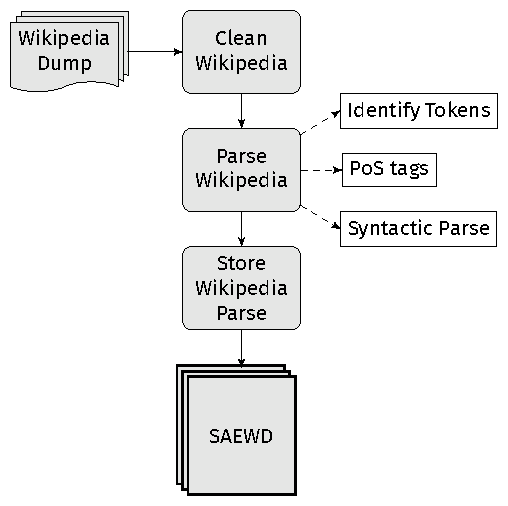
\includegraphics[scale=.8]{images/Chapitre7/flow_chart.pdf}
	\caption{The tree steps we took to build SAEWD.}
	\label{fig:flow}
%TODO change figs to Chapter4 folder!
\end{figure}

\subsection{Construction of SAEWD}
The three main steps we followed to build SAEWD are presented in Figure \ref{fig:flow}. Briefly, we have one input, which is the Wikipedia dump and one output which is the parsed snapshot. In the following we provide a detailed description of each step of the process. 

 
We begin the construction of the parsed corpus with the Wikipedia dump XML file obtained from the Wikipedia database\footnote{\url{https://dumps.wikimedia.org/enwiki}} from early November 2014. This dump  contains around 4.7 million article pages\footnote{We kept all articles available in the Wikipedia dump.}. As shown in Figure \ref{fig:flow}, we apply the following processing steps in order to yield the final parsed version.
 
\subsubsection{Cleaning Wikipedia} First, we discard Wikipedia's  tables, references and lists, markup annotations and HTML tags with the \textit{WikiExtractor} \cite{Attardi2015}  script. 
We used this tool to clean and split the content of the original XML file into 429 folders each one containing 100 files of approximately 300 kB. These files contain a certain number of complete Wikipedia articles which is automatically determined by WikiExtractor  according to the maximum possible size assigned for each file, 300 kB in our case, thus the number of articles in each file may vary. We decided to use numerous files as well as a small size to easily read their content into memory while parsing. Having multiple small files also makes it easier to handle the multi-threading aspect of our parsing tool.
We kept WikiExtractor's original folder nomenclature which assigns to each one of them a sequence of letters sorted lexicographically\footnote{We have folders named \textit{AA}, \textit{AB}, \textit{AC} and so on.}. The files containing the cleaned text is simply named \textit{wiki\_XX} where  \textit{XX} goes from 00 to 99, as we have 100 files per folder. 
It is important to note that the Wikipedia articles' titles themselves are not sorted in any specific way, as it was not in the interest of our research to have them ordered. 
Inside each cleaned file, besides the article's text, WikiExtractor keeps the original article's URL as well as its unique Wikipedia ID within an XML-like label that also doubles as  article separator. 

\subsubsection{Parsing Wikipedia} Next, once the Wikipedia dump had been cleaned, we use the Stanford CoreNLP\footnote{\url{http://nlp.stanford.edu/software/corenlp.shtml}} \cite{manning2014} analysis tools to parse all the file texts produced during the previous step. As a part of our processing pipeline, we first perform  sentence segmentation, word tokenization and lemmatization. Below, we briefly describe each of the extracted attributes. We also exemplify them in detail in Section \ref{text:description}.
\begin{itemize}
\item \textbf{PoS tagging}: we obtain the grammatical category of each word, i.e., the part-of-speech tag, using the CoreNLP default tagger, the \textit{left3words} PoS tagging model.

\item \textbf{Constituents parse}:                                                                                                                                                           
the output of this analysis is a rooted tree that represents the syntactic structure of a phrase.                                                                                  
This tree is commonly known as the constituency-based parse tree.                                                                                                                  
For each word, we store its complete path in the constituency tree.
 Specifically, we keep all the nodes of a word's own branch from the root to the word itself.
 We employ the Stanford Shift-Reduce parser.
 This path is transformed into a single line and included in SAEWD. 
\item \textbf{Dependency parse}: this attribute consists on an extracted tree that describes the types of grammatical relations between words, i.e., the dependency-based parse tree. 
The analysis was performed with the Stanford's \textit{Shift-Reduce}  parser.
% This parser is known to perform better than other Stanford parsers.                                  
 %(notably  faster and  with stronger \textit{F1} measure than the previous PCFG parser, although not as accurate as the Recurrent Neural Network system trained with semantic word vectors).
As information representation, we use the basic dependencies scheme, as we wanted to include each one of the possible dependency relations without any collapsing between them.     

\end{itemize} 	
%\section{Parsed files organization}
 Finally, once the parsing process is complete, the parsed files are stored into individual files and thus there are as much parsed files as input Wikipedia cleaned files. The parsed files keep their original name plus the \texttt{parsed} extension, e.g., \texttt{wiki\_00.parsed}. The structure within the files is described in Section \ref{section3.2}. After parsing, we found the statistics shown in Table \ref{tab:corpus_stats}.
 
\begin{table}[t]
\centering
\caption{English Wikipedia dump statistics.}
\label{tab:corpus_stats}
\begin{tabular}{lr}
{\bf Number of tokens}      & 1,889,769,908 \\
{\bf Unique tokens (types)} & 8,761,691 \\
{\bf Number of sentences}   &  84,760,512\\
{\bf Average number of tokens per sentence} & 22.30
\end{tabular}
\end{table}

\subsection{SAEWD Description}\label{text:description}
In this section we describe in detail the characteristics of SAEWD.




\begin{table*}[ht]
\centering
\caption{Extract of a Wikipedia parsed file. The phrase shown is the parse result of the previous example sentence in Figure~\ref{fig:tree_saewd} }
\label{tab:parse}
\noindent\makebox[\textwidth]{%
\begin{tabular}{llllll}
 \multicolumn{6}{l}{\textit{FILENAME wiki\_00.parsed}}                                           \\ \hline
  \textbf{token}   & \textbf{lemma}   & \textbf{POS} & \textbf{constituency}                      & \textbf{head} & \textbf{dependency} \\ \hline
 \multicolumn{6}{l}{\textit{\%\%\#PAGE Anarchism}}                                         \\ \hline
  {$\vdots$}      &      {$\vdots$}   &  {$\vdots$}   &     {$\vdots$}                              &    {$\vdots$}  &     {$\vdots$}       \\  \hline
 \multicolumn{6}{l}{\textit{\%\%\#SEN 25  9}}                                             \\ \hline
						 A       & a       & DT  & NP\_22,S\_97                      & 3    & det        \\ %\cline{2-7} 
                         great   & great   & JJ  & NP\_22,S\_97                      & 3    & amod       \\ %\cline{2-7} 
                         brigand & brigand & NN  & NP\_22,S\_97                      & 4    & nsubj      \\ %\cline{2-7} 
                         becomes & become  & VBZ & VP\_44,S\_97                      & 0    & root       \\ %\cline{2-7} 
                         a       & a       & DT  & NP\_18,NP\_20,VP\_44,S\_97        & 6    & det        \\ %\cline{2-7} 
                         ruler   & ruler   & NN  & NP\_18,NP\_20,VP\_44,S\_97        & 4    & xcomp      \\ %\cline{2-7} 
                         of      & of      & IN  & PP\_57,NP\_20,VP\_44,S\_97        & 9    & case       \\ %\cline{2-7} 
                         a       & a       & DT  & NP\_18,PP\_57,NP\_20,VP\_44,S\_97 & 9    & det        \\ %\cline{2-7} 
                         Nation  & nation  & NN  & NP\_18,PP\_57,NP\_20,VP\_44,S\_97 & 6    & nmod       \\ %	\cline{2-7} 
\hline 
      
\end{tabular}}
\end{table*}

% Please add the following required packages to your document preamble:
% \usepackage{multirow}
% \usepackage{graphicx}
\begin{table*}[ht]
\centering
\resizebox{\textwidth}{!}{%
\begin{tabular}{cl|cccc|cccc|c}
\multirow{2}{*}{\textbf{PoS Tag}} & \multirow{2}{*}{\textbf{Token}} & \multicolumn{4}{c}{\textbf{NP}} & \multicolumn{4}{c}{\textbf{DEP}} & \multicolumn{1}{l}{\textbf{SEN}} \\ 
 &  & \multicolumn{1}{c}{$ \text{NP\_22}_1 $} & \multicolumn{1}{c}{$ \text{NP\_20}_1 $} & $ \text{NP\_18}_1  $& \multicolumn{1}{c}{$ \text{NP\_18}_2 $} & nsubj\_become & xcomp\_become & nmod\_ruler & \multicolumn{1}{c}{amod\_brigand} & \multicolumn{1}{l}{$ \text{~~S}_1 $} \\ \cline{1-11} 
\multirow{3}{*}{\textbf{NN}} & \multicolumn{1}{l|}{brigand} & 1 &  &  &  & 1 &  &  & & 1 \\
 & \multicolumn{1}{l|}{ruler} &  & 1 & 1 &  &  & 1 &  &  & 1 \\
 & \multicolumn{1}{l|}{nation} &  & 1 &  & 1&  &  & 1 &  & 1 \\ \hline
\textbf{VB} & \multicolumn{1}{l|}{becomes} &  &  &  &  &  &  &  & & 1 \\ \hline
\textbf{JJ} & \multicolumn{1}{l|}{great} & 1 &  &  &  &  &  &  & 1 & 1 \\ \hline
\end{tabular}
}
\caption{Brief example of the linguistic network incidence matrix of the previous used phrase. On the left side, as on the top, we can see the metadata we store for each word (rows) and each column (hyperedges). We omit the rest of the words from the example phrase for brevity.  }
\label{ref:incidence}
\end{table*}

\paragraph{Constituency parse storage in detail}
%The  result from the constituency parse is not as straightforward to store as the other kinds of parses, i.e., the output is  a deeper tree structure than that of a dependency parse. Thus, we believe that the storage of this information in SAEWD requires a more in detail explanation. 
%In this subsection, we will describe how we stock the information concerning  the phrases' constituents. 

We will use an example to better explain the storage of the constituency-based parse tree. In Figure \ref{fig:tree_saewd} we can see the constituency parse of the phrase  \textit{A great brigand becomes a ruler of a Nation}. On the bottom of the figure, we observe the constituent's path (or branch), of the words \textit{brigand} and \textit{Nation}. As in any tree structure, each leaf node has a defined path from the root node to itself. In this example, the leaf containing the noun \textit{brigand} 
%(PoS tag \textit{NN})
 follows the bottom-up path \textit{NP22}$\rightarrow$\textit{S97}. \textit{Brigand's} parent node is a Noun Phrase (NP) node which in turn comes from the root of the tree, the Sentence node \textit{S}. We assign to each phrase chunk an identifier (22 and 97 in this case) in order to distinguish them according to their building elements as specified by the grammar rule used.
  In other words, a phrase chunk, e.g., a NP, a Verbal Phrase (VP), a Prepositional Phrase (PP), or other chunk defined by the grammar in CoreNLP, may be built from different types of PoS tags. Thus, again from Figure \ref{fig:tree_saewd}, we see that the sentence \textit{S97} is  built both from a NP and a VP chunk. 
 In a similar way, the noun phrase \textit{NP18} is produced by a determinant (DT) and a noun (NN), while  \textit{NP22} is generated by a determinant, an adjective (JJ) and a noun.
  The identification digits are obtained from the hash code that represents each chunk object inside our Java application. For each phrase-chunk tree node, we keep the last two significative figures produced by the \texttt{hashCode}\footnote{Java \texttt{hashCode} function description: \url{https://en.wikipedia.org/wiki/Java\_hashCode\%28\%29}} Java method.
%\begin{figure}[]
%\resizebox{\linewidth}{!}{%
%\begin{forest} 
%[S97
%	[NP22 [DT [A, blue text]] [JJ [great, blue text]] [NN [brigand, blue text]]]
%    [VP44 [VBZ [becomes, blue text]]
%      [NP20
%        [NP18 [DT [a, blue text]] [NN [ruler, blue text]]]
%        [PP57 [IN [of, blue text]]
%          [NP18 [DT [a, blue text]] [NN [Nation, blue text]]]]]]]
%	\node [draw,fill = blue!20,text width=21em] at (1.5,-6.8) (sparse) {\textbf{brigand} (NN): NP22$\rightarrow$S97 \\ \textbf{Nation} (NN): NP18$\rightarrow$PP57$\rightarrow$NP20$\rightarrow$VP44$\rightarrow$S97};
%\end{forest}
%}

%\caption{Constituency tree for the phrase \textit{{A great brigand becomes a ruler of a Nation}.}
%% On the bottom, we can see the bottom-up path stored for the words \textit{brigand} and \textit{Nation}.
%}
%\label{fig:tree_saewd}
%\end{figure}

\begin{figure}
\centering
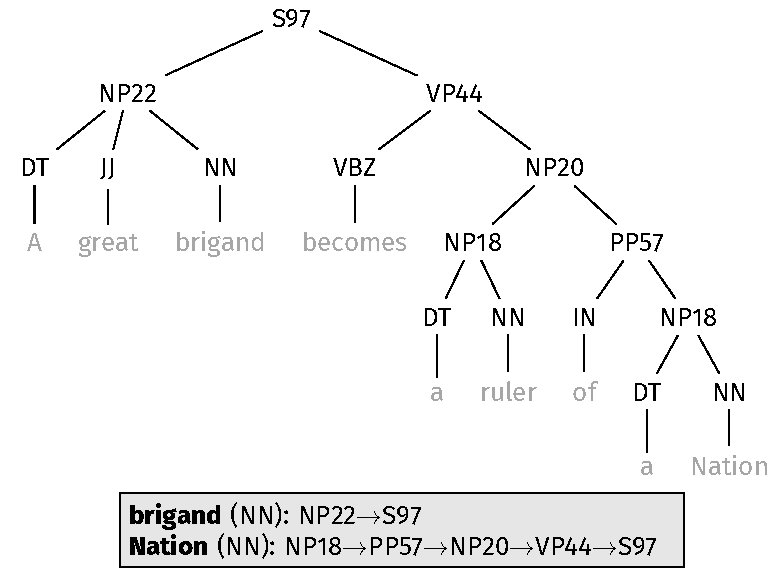
\includegraphics[width=0.8\linewidth]{images/Chapitre3/trees/tree_saewd.pdf}
\caption{Constituency tree for the phrase \textit{A great brigand becomes a ruler of a Nation}. On the bottom, we can see the bottom-up path stored for the words \textit{brigand} and \textit{Nation}.}
\label{fig:tree_saewd}
\end{figure}
 


As another example, the noun \textit{Nation} has the following bottom-up constituency path: \textit{NP18}$\rightarrow$\textit{PP57}$\rightarrow$\textit{NP20}$\rightarrow $\textit{VP44}. Indeed, the string \texttt{NP\_18,PP\_57,NP\_20,VP\_44,S\_97}, originating from the previously described path,  is the information we keep about the constituency parse for each token in the Wikipedia dump.



\paragraph{Annotation scheme}\label{section3.2}
To store the parsed text we use a scheme  inspired by that used in \cite{ATSERIAS08}. The format can be considered as a regular Tab Separated Values file  (extension tsv), with additional metadata tags. An extract from a parsed file can be observed in Table \ref{tab:parse}. 

The file includes two headers: the first one simply indicates the name of the current parse file; the second one contains the names that describe each column. The tags and columns our parsed dump contains are the following:
\begin{itemize}
\item Metadata tags:
\begin{enumerate}
\item {FILENAME}: indicates the original file used to extract the current parse, 
\item {\%\%\#PAGE}: denotes a new Wikipedia article, as well as its title, 
\item {\%\%\#SEN}: marks the beginning of a new sentence. It is followed by two integers: (1) the number of the current sentence, and (2), the number of tokens in the sentence.

\end{enumerate}

\item Parse columns for each token:
\begin{enumerate}
\item Token: the token itself,
\item Lemma: the token the canonical form,
\item POS: its part of speech tag,
\item Constituency: the bottom-up constituency path described before,
\item Head: the head index of the dependency relation the current token belongs to,
\item Constituency: the name of the grammatical relationship this token participates in as a dependent.
\end{enumerate}
\end{itemize}

Using the example phrase introduced before (Table \ref{tab:parse}), the token \textit{becomes} has \textit{become} as lemma, it is a verb, thus it has \textit{VBZ} as PoS tag, its constituency path is \textit{VP\_44,S\_97}, so it belongs to the verb phrase {VP44} which in turn comes from sentence {S97}. Finally, \textit{becomes}, being the main verb, is in this case the grammatical root of the sentence and its head is by convention determined as  zero. 

\subsection{Enriched Wikipedia-based Hypergraph}

Once SAEWD is saved to disk, we leverage its information by building a linguistic network by connecting tokens according to their interaction within the Wikipedia corpus. Given the large size of the Wikipedia corpus, we chose a sample of it to illustrate our proposed representation. We randomly selected around 200 thousand articles. %We store the incidence matrix (which is in fact a sparse matrix) on disk as a \textit{Matrix Market} format file. The metadata is stored as \textit{JSON} files. Both formats allow for an easy data lecture.


%\subsection{Enriching the Wikipedia Hypergraph with Fusion Techniques}
%

We focus now on the combination of the linguistic features contained in the model to obtain a more diverse, enriched, and less sparse representation. In this subsection, we present a practical example of what are the differences between each the three essential fusion operators (early, late and cross fusion)  and with respect to using single features independently. For sake of clarity, we focus on two types of linguistic information: lexical (with a context window  of +2-2 around each word) and syntactic (using  dependency relations).

The goals of this example are to show how the type of context affects the semantic relatedness of a given word, to get a glimpse of how heterogeneous features get combined into a single enriched representation ideally allowing us to get more knowledge about a given term, and finally, discover how the sparsity is alleviated by combining two different matrices together, especially using the late and cross fusion techniques. 

The example consists in presenting the top 5 most similar words of the target word \textit{priest} according to different representation spaces. These representation spaces are obtained using five representation matrices: the lexical features matrix ($\mlex$),  the syntactic features matrix ($\msyn$), the early fusion matrix $E(\msyn,\mlex)$, the late fusion matrix ($L_{0.5}(\ssyn,\slex)$), and finally two cross fusion matrices ($X_F(\ssyn,\mlex)$ and $X_F(\slex,\msyn)$). We  report the sparsity level of each matrix (percentage of zero values in the matrix) obtained. 

The procedure to obtain said similar words consist in calculating a cosine-similarity matrix for each of the five fusion representations. In some cases, as in late fusion and cross fusion, this step is implicit as in this example, these operators already require the computation of similarity matrices (see Equations \ref{eq:late-fusion} and \ref{eq:xfusion}).

The  most similar terms to the target word can be seen in Table \ref{tab:priest}. We note that in this example we are not interested in determining the quality of the semantic related words discovered with each representation space. Even more, it seems hard to determine the semantic-relatedness quality of these similar (\textit{similar} in the sense of cosine similarity) words. Still, we can say that, as expected, the words seem to be semantically related in a large sense.

As discussed by \cite{LevyG14}, lexical features seem to give words that are semantically related in a larger sense, in this example, religion related terms. On the other hand, dependency based relations similarities tend to discover functional words or words that are of the same \textit{semantic type}.
With respect to early and late fusion, while the similar words found are already known, we discover new terms that were until now unknown which seem to be semantically related, such as \textit{relic} and \textit{seer}. Concerning the cross fusion, in this case cross feature fusion, both transferring from the syntactic to the lexical similarity matrix and the other way around, we see that we also found previously seen words while discovering yet another couple of related words: \textit{monk} and \textit{chorus}. It is also clear how by selecting to transfer information from the syntactic matrix (fifth column) we get functionally related terms (occupations in the church or in a power structure) while on the sixth column (transfer from lexical to syntactic), we get mostly words that correspond to a broader similarity domain.

In Table \ref{tab:priestSims} we present again the top 5 similar terms to the word \textit{priest}.  This time using similarity matrices as representation spaces. The overall behavior described above regarding the nature of the semantic relations is also kept in this representation spaces.

With regard to alleviating the data sparsity (indicated below the header of each column as the percentage of non-zero values in the matrix) it is quite obvious that by using a similarity matrix we densify the space by means of a matrix multiplication, which is the case of both cross fusion operators (columns four and five of Table \ref{tab:priest}): we pass from a sparsity of {5.49}\% in the lexical matrix and {4.97}\% in the syntactic matrix to  {16.75}\% and {13.45}\% in the cross fusion matrices, respectively. 
%The large increment of density in the late fusion representation is obviously due to the use of similarity matrices in this operation, which usually tend to be dense matrices.
%
Furthermore, for the cross feature fusions $X_F$, while we also employ a similarity matrix, we stay in the same space (same number of dimensions) of the feature matrix, while more than doubling the density of the space at the same time. 


On the other hand, the same reduction of sparsity is achieved while using similarity matrices, (in Table \ref{tab:priestSims}). Originally having 75.25\% and 60.64\% sparsity using the lexical and syntactic similarity matrices respectively, we get to a maximum of 87.22\% using cross similarity fusion going from syntactic to lexical information $X_S(S^S, S^L)$.


% Please add the following required packages to your document preamble:
% \usepackage{booktabs}
\begin{table}[]
\centering

\begin{tabular}{@{}llllll@{}}
\toprule
                           & \textbf{\begin{tabular}[c]{@{}l@{}}Lexical\\ Features\\(5.49\%)\\$\mlex$\end{tabular}}              
                           & \textbf{\begin{tabular}[c]{@{}l@{}}Syntactic\\ Features\\(4.97\%)\\$\msyn$\end{tabular}}        
                           & \textbf{\begin{tabular}[c]{@{}l@{}}Early\\ Fusion\\(5.23\%)\\$E(\mlex, \msyn)$\end{tabular}}                
                           & \textbf{\begin{tabular}[c]{@{}l@{}}$X_F$\\Fusion\\(16.75\%)\\$X_F(\ssyn, \mlex)$\end{tabular}}   &
                           \textbf{\begin{tabular}[c]{@{}l@{}}$X_F$\\Fusion\\ (13.45\%) \\$X_F(\slex, \msyn)$\end{tabular}}                 \\ \midrule
\multicolumn{1}{c}{priest} & \begin{tabular}[c]{@{}l@{}}priests\\ nun\\ canton\\ sailor\\ burial\end{tabular} & \begin{tabular}[c]{@{}l@{}}monk\\ regent\\ aedile\\ seer\\ meek\end{tabular} & \begin{tabular}[c]{@{}l@{}}sailor\\ regent\\ nuclei\\ nun\\ relic\end{tabular} & \begin{tabular}[c]{@{}l@{}}vassal\\ regent\\ nun\\ sailor\\ monk\end{tabular} & \begin{tabular}[c]{@{}l@{}}sailor\\ fluent\\ dean\\ nuclei\\ chorus\end{tabular} \\

 \bottomrule

\end{tabular}
\caption{Target word \textit{priest} and its top 5 most similar words using different representation matrices. The sparsity level (percentage of non-zero values) of each representation is shown below the header of each column.}
\label{tab:priest}
\end{table}

\begin{table}[]
\centering

\begin{tabular}{@{}lllllll@{}}
\toprule
                           & \textbf{\begin{tabular}[c]{@{}l@{}}Lexical\\ Similarity\\(75.25\%)\\$S^L$\end{tabular}}              & \textbf{\begin{tabular}[c]{@{}l@{}}Syntactic\\ Similarity\\(60.64\%)\\$S^S$\end{tabular}}        & \textbf{\begin{tabular}[c]{@{}l@{}}Early\\ Fusion\\(67.94\%)\\$E(S^L, S^S)$\end{tabular}}                & \textbf{\begin{tabular}[c]{@{}l@{}}Late\\ Fusion\\(83.17\%)\\$L(S^L, S^S)$\end{tabular}}                 & \textbf{\begin{tabular}[c]{@{}l@{}}$X_S$\\ Fusion\\(87.22\%)\\$X_S(\ssyn, \slex)$\end{tabular}}  &
                           \textbf{\begin{tabular}[c]{@{}l@{}}$X_S$\\
                           Fusion\\(79.69\%)\\$X_S(\slex,\ssyn)$\end{tabular}}                 
                           \\ \midrule
\multicolumn{1}{c}{priest} 
& \begin{tabular}[c]{@{}l@{}}wholly\\burial\\monk\\lingua\\nuclei\end{tabular} &
\begin{tabular}[c]{@{}l@{}}regent\\ coach\\ broker\\ dream\\tailor\end{tabular} & \begin{tabular}[c]{@{}l@{}}regent\\slang\\ broker\\rebel\\tiger\end{tabular} & \begin{tabular}[c]{@{}l@{}}regent\\slang\\ seer\\ tutor\\cradle\end{tabular} & \begin{tabular}[c]{@{}l@{}}regent\\vassal\\vizier\\leader\\result\end{tabular} & \begin{tabular}[c]{@{}l@{}}sailor\\nuclei\\nun\\canton\\burial\end{tabular} \\

 \bottomrule

\end{tabular}
\caption{Target word \textit{priest} and its top 5 most similar words using different representation similarity matrices. The sparsity level (percentage of non-zero values) of each representation is shown below the header of each column.}
\label{tab:priestSims}
\end{table}


%\paragraph{Discussion}
%Concerning the computation time, SAEWD takes around 40 hours to be produced using a general purpose laptop (Intel i7 4700MQ with 4 cores, 8 GB and Linux Mint 17 as operative system). Most of the time is taken by the parsing step. 
%
%We verified the consistency of the corpus built by analyzing a sample of 20 Wikipedia articles. The output of CoreNLP and the information contained in the corpus match.



\section{Conclusion}

In this chapter  we analyzed the state of the art of linguistic network-based approaches to semantic similarity task from a graph-centric point of view. We reviewed the techniques in terms of its graph characteristics, from their structure to the algorithms employed. Among the literature covered, certain non-explored research paths were identified, namely the lack of syntactic data on the networks employed, and therefore, a homogeneous network nature that only allows for relations of a unique type. 

We addressed these paths with the proposition of a fusion enriched hypergraph linguistic model that is able to hold heterogeneous language information while allowing its combination and alleviating the data sparsity.  This structure allows the integration multiple kinds of information and has potential in terms of which algorithms it can be used with. The three levels of contexts we integrated in the model (sentence lexical co-occurrence, dependency function co-occurrence, and constituent-membership co-occurrence) aim to cover distinct levels of semantic relatedness. We noted the challenges of dealing both with textual data sparsity and leveraging the heterogeneity of the hypergraph. To alleviate both concerns, we propose the use of fusion functions, introduced also in this chapter. The structure of the hypergraph is also an important characteristic that we can use to find groups of semantically related words within a corpus. Finally, we presented a materialization of a corpus, a portion of the English Wikipedia, as the linguistic network we proposed.




\chapter{Applications to named entity recognition and word sense disambiguation} 
\label{chap:wsd}
\begin{abstractchap}
This chapter presents the experiments we performed as applications of the proposed model. On the first subsection, we use well-known methods to solve named entity recognition while using fusion enriched representation spaces. We show that these kinds of representations, leveraging heterogeneous information and alleviating its data sparsity, are useful to improve the performance of the task. Indeed, our results on three different datasets using enriched representations are better than those of the baselines we propose, and more importantly, our results show that the combination of textual features indeed improves the performance compared to single feature and the trivial feature concatenation. We also give a detailed analysis into how the fusion operations get to improve the performance of the task at hand.

In the second subsection, we change the NLP task to word sense induction and disambiguation. First, we apply the same fusion operations as before to solve the task using an existing literature approach. Our experiments on two different corpora show that the improvements shown in named entity recognition are consistent in word sense induction and disambiguation. Secondly, we propose a method to exploit the structure of the network within our linguistic model. 
Although this approach has been studied before, we improve over the previous  literature results while having a reduced number of parameters and employing heterogeneous features to solve the task. We also analyze the results obtained according to the  type of word studied, whether nouns or verbs, and according to the effect of the use of either lexical or syntactical information.


%Secondly, in the second section of the chapter, we explore the use of well-known multi-modal fusion techniques to solve two prominent Natural Language Processing tasks. Specifically, we focus on solving Named Entity Recognition and Word  Induction and Disambiguation by applying feature-combination methods that have already shown their efficiency in the multi-media analysis domain. We present a series of experiments employing fusion techniques in order to combine textual linguistic features. 
%Furthermore, we perform an extensive analysis on the importance of each feature relevance with respect to the senses and classes discovered in WSI/WSD and NER, respectively.

\end{abstractchap}

\minitoc
\section{Introduction}
In this applications chapter we set to solve two natural language processing tasks using as data source corpora in the form of the model described in Chapter \ref{chap:ling_net}. We address the tasks of Named Entity Recognition (NER) and Word Sense Induction and Disambiguation (WSI/WSD). Both tasks are located on the  semantics sub-domain of NLP. 

These experiments represent the third and final contribution of this thesis, after introducing the theoretical fusion enriched model in the previous chapter. Indeed, this contribution is the continuation of our set of propositions, as shown in Figure \ref{fig:main_diag2}. We employ both a fusion enriched and a raw hypergraph network based on benchmark corpora to validate the utility of our proposals.

The general objectives of the experiments described below are two: (1) to test the effectiveness of using fusion enriched representations to solve NLP tasks, while combining heterogeneous information and densifying the feature space;  and (2), to leverage the structure of a network built using the hypergraph structure described before.

 %By making use of the network we want to test the effectiveness of using different types of linguistic features. 
There are two main parts  in this chapter. First we address NER, we study how the different types of fusion operations affect the performance of the task. We train well-known classification algorithms with representations obtained from fusion operations.  According to our results, we find that it is indeed interesting to combine different types of features into a single representation space. We also delve into a result's analysis to try to understand the reason behind the improvement using fusion techniques.

The second part deals with WSI/WSD. This subsection is divided in two segments. First, once we determined that combining features is interesting for NER, we want to verify that this combined representations are indeed useful for other NLP tasks, such as WSI/WSD. As before, we use a literature learning technique with the representation obtained by the combination of available features. Our results show that the fusion enrichment is useful also to solve WSI/WSD.

Secondly, we leverage the structure within the hypergraph resource to solve WSI/WSD. Briefly, the goal is to detect important words, according to their connections with other words, and extract their neighborhood to determine possible senses  within the network. While this method has been used before, we improve the performance and reduce the number of parameters employed by those literature methods. We also study the effect of using different types of linguistic information, namely lexical and syntactic contexts.

At the end of the chapter we conclude by discussing the experiments performed, their limitations and  future improvements and further research. 

\begin{figure}
\centering
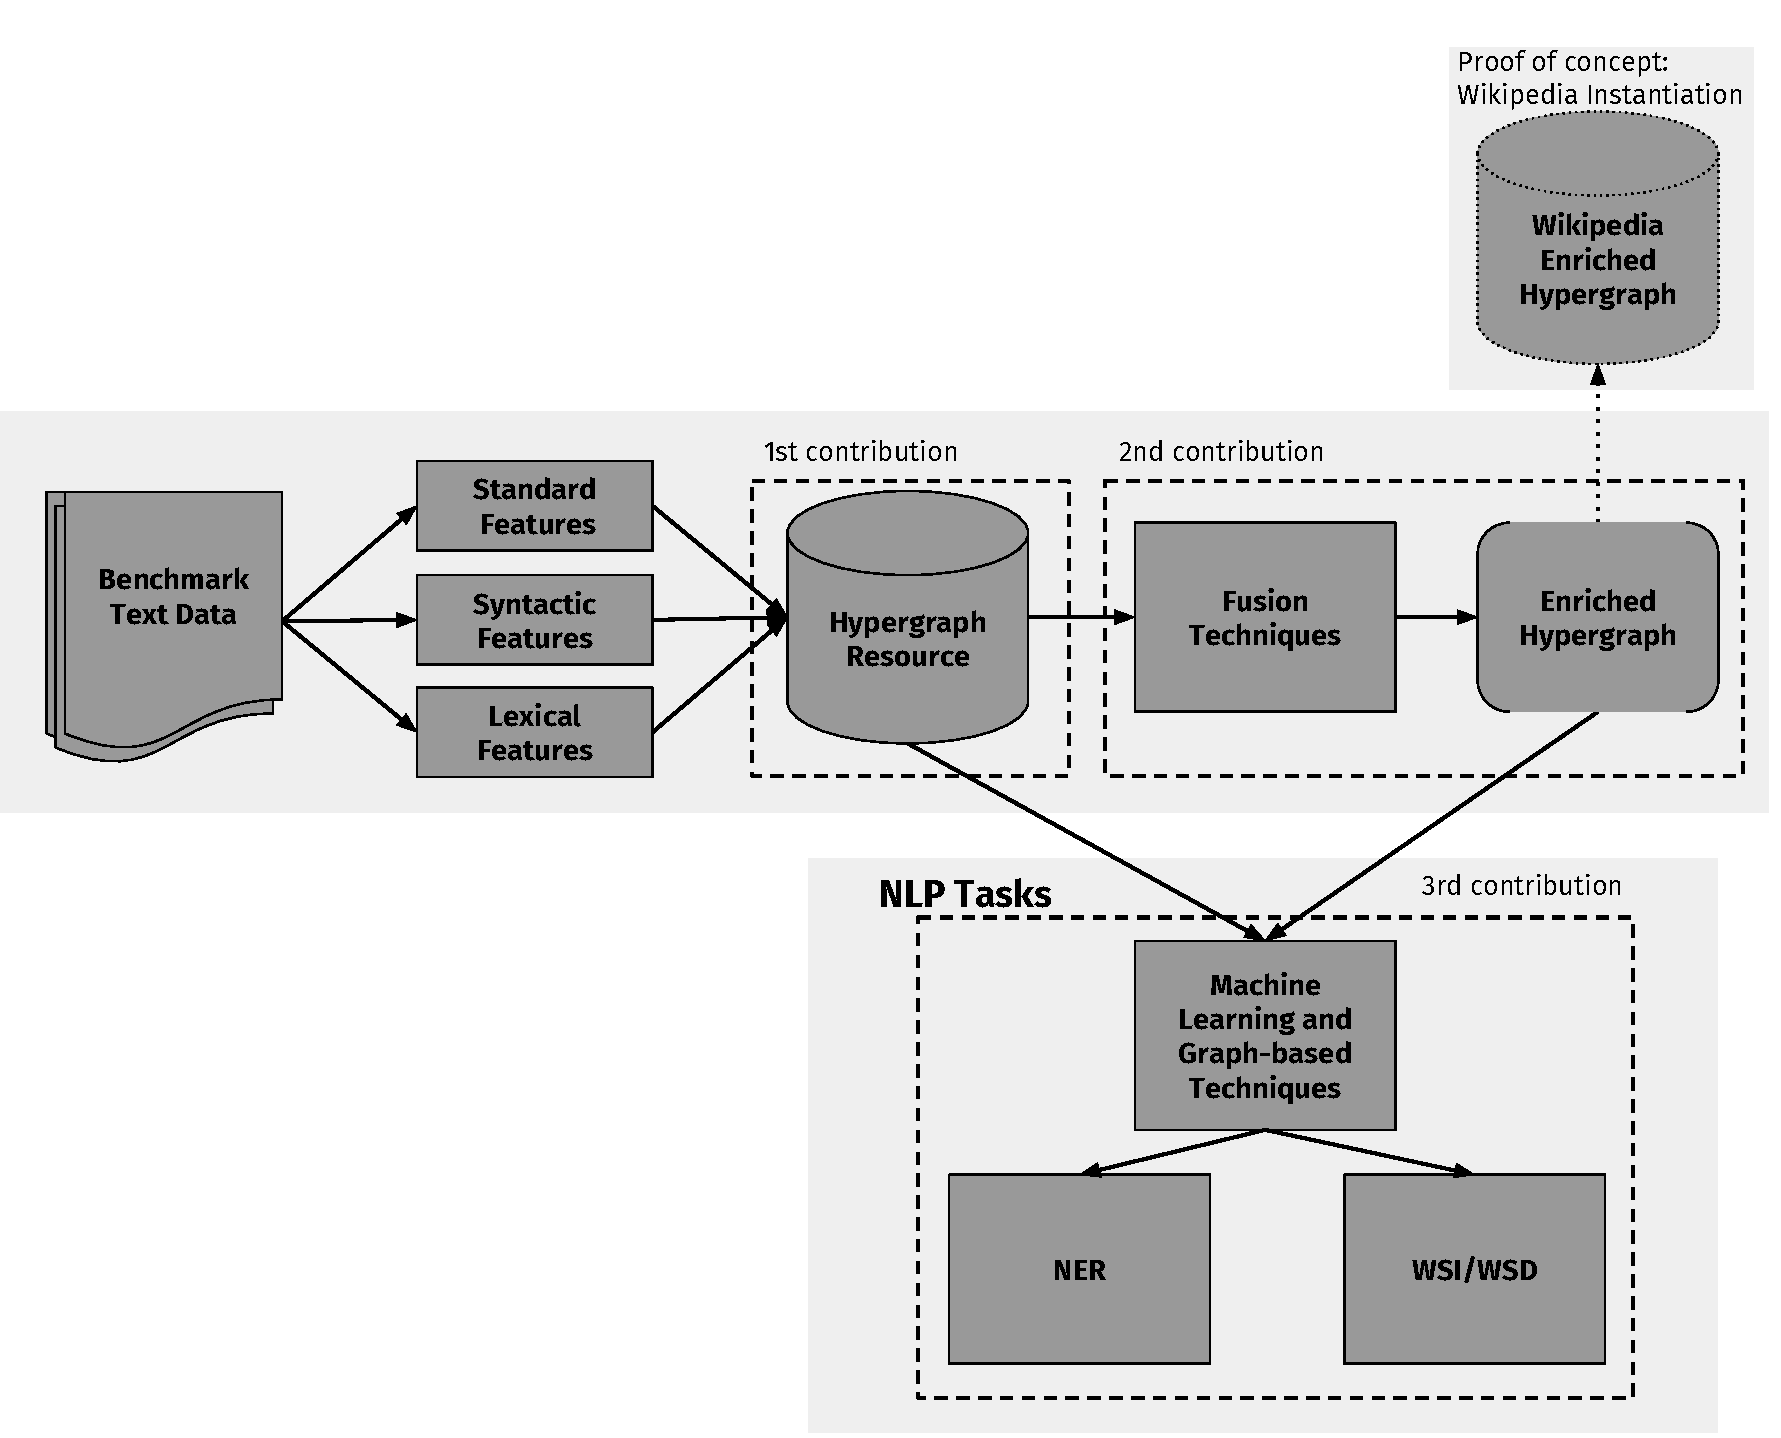
\includegraphics[width=.9\linewidth]{images/Chapitre4/main_diag2.pdf}
\caption{Complete description of the three contributions of this work. In this chapter we focus on the third contribution, addressing WSD/WSI and NER with the model proposed in the previous chapter.}
\label{fig:main_diag2}
\end{figure}

\section{First Application: Named Entity Recognition}
\label{sec:ner}


 NER goal is to automatically discover, within a text, mentions that belong to a well-defined semantic category. The classic task of NER involves detecting, within a text, entities of type Location (LOC), Organization (ORG), Person (PER), Miscellaneous (MISC), or if the term is not an even an entity, assigning them a (O) label. The task is of great importance for more complex NLP systems, e.g, relation extraction, opinion mining \cite{nadeau2007survey}.  
 
 Generally, two common solutions to NER involve the use of matching patterns, created manually or extracted in a semi-automatically fashion\cite{gupta2015distantly}; or more popularly, by training a supervised machine learning algorithm with large quantities of annotated text \cite{mining12Book} . The latter being the currently more popular solution to this task. As is usual with other NLP tasks, NER  requires textual features to represent words in order to determine their role within a phrase. We propose to build representations based on our fusion enriched hypergraph model.


Usually, representations employed for NER are obtained from the surrounding context of the words in the  input corpus. Mainly,  two types of representations are used: lexical and syntactic. As we know, the first type requires no extra information than that contained already in the analyzed text itself. The second type, syntactic features  are based on part of speech tags, phrase constituents information, and syntactical functionality between words, the later portrayed by syntactical dependencies. Likewise, there are specific features that are particular to one task are also be employed.


The main intuition of these experiments is that word similarities may be found at different levels according to the type of features employed. In order to exploit these similarities, we leverage our fusion enriched framework. Specifically, in our experiments, we try to mutually complement independent representations by utilizing said fusion techniques to generate a single feature space that improves the performance of NER, specially compared to the using features independently and the trivial feature concatenation (early fusion). Consequently, the main goal is to assess the effectiveness of simple, yet untested fusion techniques and their combination.

%The rest of the chapter is organized as follows: in section \ref{chap6:back}, we go into further details about fusion techniques. 
%%as well as its application in the NLP domain. 
%We introduce the fusion operators that we use in our experiments in section \ref{chap6:application}. Then, in section \ref{chap6:expes} we show the effectiveness of the presented methods by testing them on NER and WSI/WSD and their respective datasets. Finally, in section \ref{chap6:conclusion} we present our conclusions and future directions to explore. A more general overview on fusion for multimedia analysis can be found in \cite{AtreyHEK10}.


We consider the first three types of fusion techniques described in subsection \ref{sec:fusion} (early fusion, late fusion and cross fusion) as the building blocks to the experiments we conduct.  While we work with a single modality, i.e., textual data, we consider the different kinds of features extracted from it as distinct modalities. Our intuition being that the semantic similarities among words in these different spaces can be combined in order to exploit the latent complementarity between the lexical and syntactical representations. We also find new combinations empirically. Nonetheless, as we will show, their effectiveness replicates to different datasets and NLP tasks. 

The specific methods used to solve both NER and WSI/WSD (in the following subsection) are already known to be robust. Our work focus specially on the generation of new representation spaces.
% Using well-proven methods to solve both WSI/WSD and NER, so that the learning part of our experiments is known to be robust.
%The fusion should therefore improve the performance of the NLP tasks at hand, first NER and later on WSI/WSD

\subsection{Fusion Enriched Representations}
\label{chap6:application}
 Our first goal in this subsection is to assess the effectiveness of the classic fusion methods and then, as a second goal, to propose new combinations that yield better outcomes in terms of performance than the simpler approaches. The new combinations are found through experimentation. Nonetheless, as we will show, their effectiveness replicates to different datasets and NLP tasks. 





\begin{figure}[t]
\centering
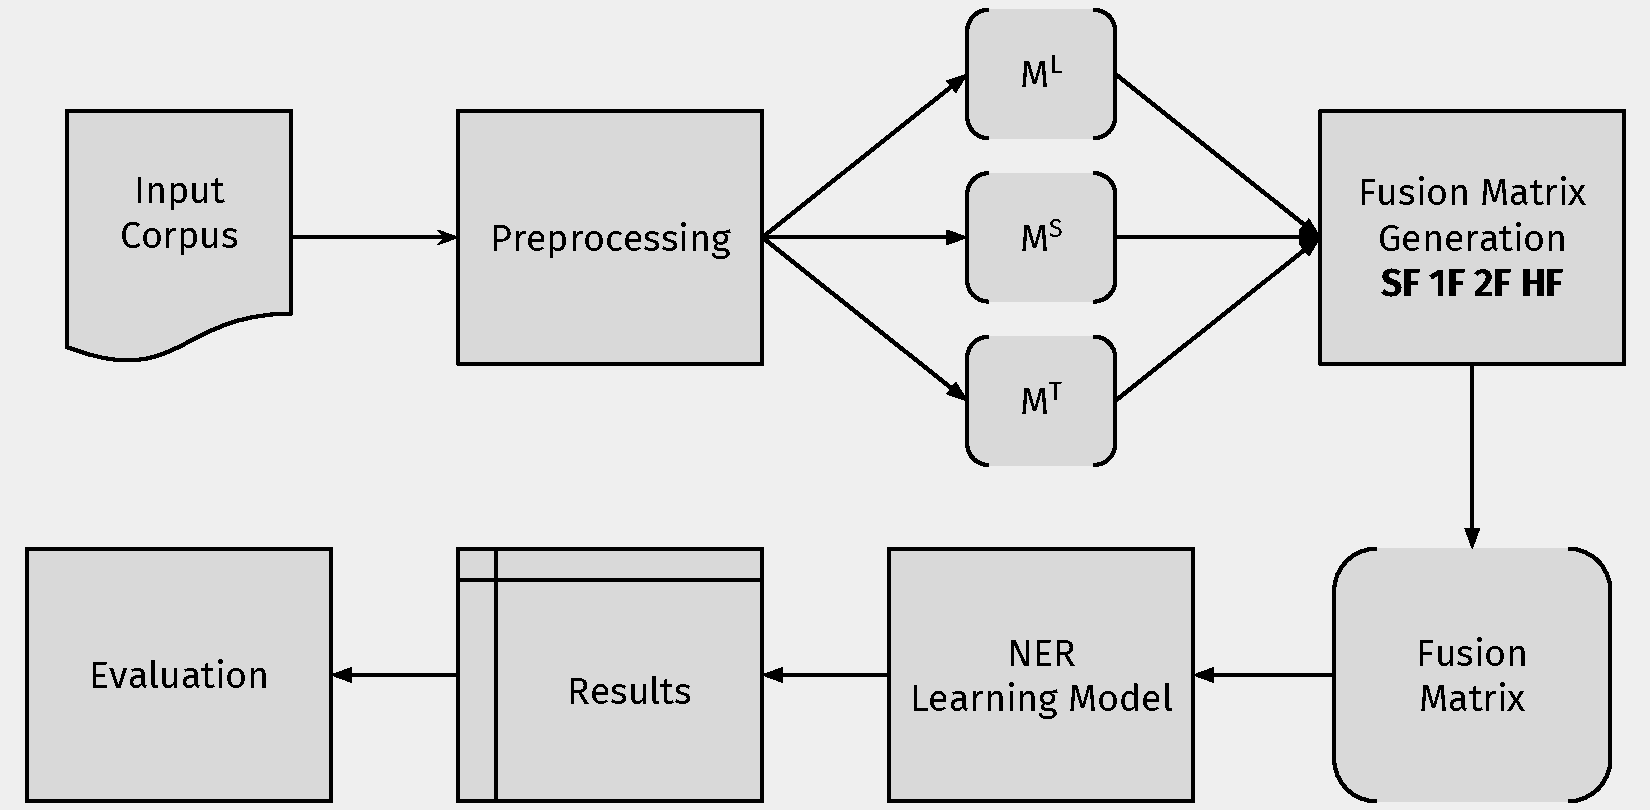
\includegraphics[width=0.85\linewidth]{images/Chapitre4/diag_metodoNER.pdf}
\caption{Steps followed on our fusion-enriched representations for NER  experiments. First the corpus is preprocessed, then features are extracted from the text. A fusion matrix is generated, which in turn is used as input to a learning algorithm. Finally, the system yields its results and to be analyzed.}
\label{fig:diagmetodo}
\end{figure}

The experiments we carry on consist in generating fusion matrices that will serve as input to a learning algorithm in order to solve NER. These input feature matrices are based upon lexical, syntactical, or other NER standard types of representation. The procedure can be sen in Figure \ref{fig:diagmetodo}.

\paragraph{Representation Spaces}\label{sec:rep_spaces}
In  Chapter \ref{chap:ling_net} we presented the fusion operators to be used in our experiments. Below we detail the three types of features matrices used to generate the fusion-enriched combinations that describe the words of the corpus tested.
\subparagraph{Lexical Matrix (L)}
For each token in the corpus, we use a lexical window of two words to the left and two words to the right, plus the token itself. Specifically, for a target word $w$, its lexical context is $(w_{-2}, w_{-1}, w, w_{+1}, w_{+2})$. This type of context features is typical for general systems studying the surroundings of a word and in particular for the named entity recognition task \cite{Daume2006,Nothman2009,RatinovR09}. 
 We retake the example phrase from \cite{LevyG14}, the lexical-based features of the phrase \textit{Australian scientist discovers start with telescope}, are shown in Table \ref{tab:lex-contextos}.
 
\begin{table}[ht]
\centering
\begin{tabular}{ll}
\hline 
 \textbf{Word} & \textbf{Features} \\ 
\hline 
Australian & word:Australian, word+1:scientist, word+2:discovers\\ 
scientist  &  word-1:Australian, word:scientist, word+1:discovers, word+2:star\\ 
discovers & word-2:Australian, word-1:scientist, $\dots$, word+2:telescope \\ 
star & word-2:scientist, word-1:discovers, word:star, $\dots$, word+2:telescope \\ 
with & word-2:discovers, word-1:star, word:with, word+1:telescope \\ 
telescope  &  word-2:star, word-1:with, word:telescope \\ 
\hline \
\end{tabular} 

\caption{Lexical features corresponding to the phrase \textit{Australian scientist discovers start with telescope}.}
\label{tab:lex-contextos}
\end{table} 

\subparagraph{Syntactical Matrix (S)}
Based on the syntactic features used in   \cite{LevyG14,Panchenko2017}, we derive contexts based on the syntactic relations a word participates in, as well as including the part of speech (PoS) of the arguments of these relations. Formally, for a word $w$ with modifiers $m_1, \dots, m_k$ and their corresponding PoS tags $p_{m_1}, \dots, p_{m_k}$; a head $h$ and its corresponding PoS tag $p_h$, we consider the context features $(m_1, p_{m_1}, lbl_1), \dots, \allowbreak (m_k, p_{m_k}, lbl_k), \allowbreak (h,p_h,lbl\_inv_h)$. In this case, $lbl$ and $lbl_{inv}$ indicate the label of the dependency relation and its inverse, correspondingly. Using syntactic dependencies as features should yield more specific similarities, closer to synonymy, instead of the broader topical similarity found through lexical contexts.

For the phrase \textit{Australian scientist discovers start with telescope} the dependency-based context is shown in Table \ref{tab:syn-contexts}.
\subparagraph{NER Standard Features Matrix (T)}
The features used for NER are based roughly on the same as those used in \cite{Daume2006,Balasuriya2009}. The feature set consists of: the word itself, whether the word begins with capital letter, prefix and suffix up to three characters (also within a window of two words to the left and two words to the right), and the PoS tag of the current word. These features are considered to be standard in the literature. We note that the matrix generated with these features is exclusively used in the experiments regarding NER.	

\begin{table*}
\centering
\begin{tabular}{ll}
\hline 
 Word & Contexts \\ 
\hline 
Australian & scientist/NN/amod\_inv \\ 
scientist  &  Australian/JJ/amod, discovers/VBZ/nsubj\_inv\\ 
discovers & scientist/NN/nsubj, star/NN/dobj, telescope/NN/nmod:with \\ 
star & discovers/VBZ/dobj\_inv \\ 
telescope  &  discovers/VBZ/nmod:with\_inv \\ 
\hline \
\end{tabular} 
\caption{Syntactic contexts corresponding to the phrase \textit{Australian scientist discovers start with telescope}.}
\label{tab:syn-contexts}
\end{table*}


\paragraph{Learning Methods}
NER being a supervised learning task, we use an averaged structured perceptron  \cite{Collins2002,Daume2006} (see Section \ref{sec:perceptron}) to determine the tags of the named entities. We considered logistic regression and linear SVM. For the main experiments, we chose the perceptron because of its performance and the lower training time. On the other hand, for the analysis of the results, we use a logistic regression as it is considerably easier to interpret its results, keeping in mind that our goal is to give some insights regarding the usefulness of our fusion methods.




\subsection{Experiments and Evaluation}
\label{chap6:expes}

We experiment with the four levels of fusion discussed before: Single Features (SF), First-degree Fusion (1F), Second-degree Fusion (2F) and Higher-degree Fusion (HF). The representation matrices for NER come from lexical context features $\mlex$, syntactical context features $\msyn$ or standard features $\mstd$.  On the other hand, experiments on WSI/WSD exclusively employ matrices $\mlex$ and $\msyn$.

We recall that our first goal is to compare the efficiency of the primary  fusion techniques applied to   named entity recognition. Then, we empirically determine a fusion combination operator able to leverage the complementarity of the features used.

To this end, we evaluate the aforementioned 4 fusion levels. We note that the fusion combinations in the third and fourth level (2F and HF) are proposed based on the results obtained in the previous levels. In other words, in order to reduce the number of experiments, we restrict our tests to the best performing configurations. This is due to the large number of possible fusion combinations that can be tested.
% (an argument to a fusion operation may be any valid output of a second fusion operation).



\paragraph{Preprocessing}

As is usual when preprocessing text before performing named entity recognition, \cite{RatinovR09}, we normalize tokens that include numbers. For example, the token 1980 becomes *DDDD* and 212-325-4751 becomes *DDD*-*DDD*-*DDDD*. This allows a degree of abstraction to tokens that contain years, phone numbers, etc. We do not normalize punctuation marks.

\paragraph{Features}
The linguistic information we use is again extracted with the Stanford's CoreNLP parser. We recall that the features used for these experiments on NER are those described before: lexical, syntactic and standard features, i.e., $\mlex$, $\msyn$, and $\mstd$, respectively. 

\paragraph{Test Datasets}We work with three corpus coming from different domains:
\begin{itemize}
\item [(1)] CoNLL-2003 (CONLL): This dataset was used in the language-independent named entity recognition CoNLL-2003 shared task \cite{SangM03}. It contains selected news-wire articles from the Reuters Corpus. Each article is annotated manually. It is divided in three parts:  training (\textit{train}) and two testing sets (\textit{testa} and \textit{testb}). The training part contains 219,554 lines, while the test sets contain 55,044 and 50,350 lines, respectively. The task was evaluated on the \textit{testb} file, as in the original task.
\item [(2)]WikiNER (WNER): A more recent dataset \cite{Nothman2009} of selected English \allowbreak Wikipedia articles, all of them annotated automatically with the author's semi-supervised \allowbreak method. In total, it contains 3.5 million words from an unspecified number of articles. 
\item[(3)] Wikigold (WGLD): Also a corpus of Wikipedia articles \cite{Balasuriya2009}. Nonetheless, this one was annotated manually. This dataset is the smaller, using 149 articles and 41,011 words. We used this corpus to validate human-tagged Wikipedia text. These three datasets are tagged with the same four types of entities: Location, Organization, Person and Miscellaneous. Otherwise, while it is faster to train models with this corpus, it may be the case that they are not able to properly fit the data given its size, and thus performance is lower than the other datasets.

The three of these datasets employ the BIO text segment tagging schemes. This tag set suggests that a word is in the \textbf{B}eginning, \textbf{I}nside, or \textbf{O}utside of a named entity. Indeed, given that there are four categories, person (PER), location (LOC), organization (ORG) and miscellaneous (MISC), there are indeed 9 different classes (B and I for each category plus O).



\end{itemize}
%
\paragraph{Evaluation Measures}
We evaluate our NER models following the standard CoNLL-2003 evaluation script. Given the large amount of experiments we carried out and to reduce the number of reported results, we report exclusively the total F-measure for the four types of entities (Location, Organization, Person, Miscellaneous). WNER and WGLD datasets are evaluated on a 5-fold cross validation.

\subsection{Results and Discussion}
We present in this subsection the results obtained in the named entity recognition task, while employing the 4 levels of fusion proposed in the previous section.

In contrast to other related fusion works \cite{Ah-PineCC15,ClinchantAC11,GialampoukidisM16}, we do not focus our analysis on the impact of the parameters of the fusion operators. Instead, we focus our analysis on the effect of the type of linguistic data being used and how, by transferring information from one feature type to another, they can be experimentally recombined to generate more complete representations.

Regarding the fusion operators' parameters, we empirically found the best configuration for $\beta$, from late fusion $L_\beta(A,B) = \beta \cdot A + (1 - \beta)\cdot B$, to be $\beta=0.5$. This implies that an equal combination is the best linear fusion for two different types of features.

In respect of the $\gamma$ parameter, used in cross fusion $X_{\gamma}(A,B) = \mathbf{K}(A,\gamma) \times B$, we set $\gamma=5$. This indicates that just few high quality similarities attain better results than utilizing a larger quantity of lower quality similarities.

\begin{table}[!tbp]
\centering
\caption{NER F-measure results using the Single Features over the three datasets. These values serve as a first set of baselines. Results are obtained with the structured perceptron algorithm.}
\label{tab:ner-blines}
\begin{tabular}{@{}lccc@{}}
\toprule
$A$                           & \multicolumn{3}{c}{\textbf{Single Features}} \\ \midrule
                & \textbf{CONLL}    & \textbf{WNER}     & \textbf{WGLD}    \\ \cmidrule{2-4}
$\mstd$                        & 77.41    & 77.50    & 59.66   \\
$\mlex$                       & 69.40    & 69.17    & 52.34   \\
$\msyn$                        & 32.95    & 28.47    & 25.49   \\ \bottomrule
\end{tabular}

\end{table}
\paragraph{Single Features}
Looking at Table \ref{tab:ner-blines}, we see that the best single features (SF), in terms of F-measure come from the standard representation matrix $\mstd$. This is not surprising as these features, simple as they may be, have been used and proved extensively in the NER community. On the other hand, $\mlex$ performs relatively well, considering it only includes information contained in the dataset itself. Nevertheless, this kind of representation is the foundation of most word embedding techniques used nowadays.
While we expected better results from the syntactical features $\msyn$, as they are able to provide not only general word similarity, but also functional, getting close to synonymy-level \cite{LevyG14},  we believe that the relatively small size of the datasets do not provide enough information to generalize 


\begin{table}[!t]
\centering
\setlength\tabcolsep{2pt}

\caption{NER F-measure results using first degree fusion (1F). Operators in column $B$ are either indicated on the table or specified as follows. In $X_FF$, depending on the dataset tested,  ${b}^*_{\scriptscriptstyle X_FF}$ takes the matrix from the set $\{\mlex, \mstd\}$ which yields the best performing result. In $X_SF$, $\hat{b}_{\scriptscriptstyle X_SF}^{*}$ corresponds to the best performing matrix in $\{\slex,\ssyn\}$. These configurations serve as the main set of baseline results. Results are obtained with the structured perceptron algorithm.}
\label{tab:ner-1d}
\centering
%\tablewidth=\textwidth
\begin{tabular}{@{}llccc@{}}
\toprule
    $A$      &    $B$       & \multicolumn{3}{r}{\textbf{Early Fusion (EF)} }                                            \\ \midrule
          &           & \textbf{CONLL}                      & \textbf{WNER}                      & \textbf{WGLD}                      \\ \cmidrule{3-5}
          
$\mlex$ & $\msyn$ & 72.01                      & 70.59                     & 59.38                     \\
$\mlex$ & $\mstd$ & 78.13                      & 79.78                     & 61.96                     \\
$\msyn$ & $\mstd$ & 77.70                      & 78.10                     & 60.93                     \\
$\mlex$ & $E(M^S, M^T)$ & \textbf{78.90}                      & \textbf{80.04}                     & \textbf{63.20}                   \\
\midrule
          &           & \multicolumn{3}{r}{\textbf{Late Fusion (LF)} }                                             \\
\midrule     
          &           & \textbf{CONLL}                      & \textbf{WNER}                      & \textbf{WGLD}                      \\ \cmidrule{3-5}
$\slex$ & $\ssyn$ & \textbf{61.65}                      & 58.79                     & 44.29                     \\
$\slex$ & $\sstd$ & 55.64                      & \textbf{67.70}                     & 48.00                     \\
$\ssyn$ & $\sstd$ & 50.21                      & 58.41                     & \textbf{49.81}                     \\
\midrule
          &           & \multicolumn{3}{r}{\textbf{Cross Feature Fusion ($\mathbf{X_FF}$)}} \\
\midrule
          &           & \textbf{CONLL}                      & \textbf{WNER}                      & \textbf{WGLD}                      \\ \cmidrule{3-5}
$\slex$ &$\mstd$        & 49.90                      & \textbf{70.27}                     & \textbf{62.69}                    \\
$\ssyn$ & $\mstd$ & 47.27                      & 51.38                     & 48.53                     \\
$\sstd$ & ${b}^*_{\scriptscriptstyle X_FF}$        & \textbf{52.89}                      & 62.21                     & 50.15                     \\
\midrule
          &           & \multicolumn{3}{r}{\textbf{Cross Similarity Fusion ($\mathbf{X_SF}$)}}  \\
\midrule
          &           & \textbf{CONLL}                      & \textbf{WNER}                      & \textbf{WGLD}                      \\ \cmidrule{3-5}
$\slex$ & $\sstd$ & 27.75                      & \textbf{59.12}                     & 38.35                     \\
$\ssyn$ & ${b}_{\scriptscriptstyle X_SF}^{*}$       & 36.87                      & 40.92                     & 39.62                     \\
$\sstd$ & ${b}_{\scriptscriptstyle X_SF}^{*}$        & \textbf{41.89}                      & 52.03                     & \textbf{39.92}                     \\ \bottomrule
\end{tabular}
\end{table}

\paragraph{First Degree Fusion }
In Table \ref{tab:ner-1d} we present the first degree fusion level (1F). The best performance is obtained by trivially concatenating the representation matrices. This baseline proved to be the toughest result to beat. Late fusion does not perform well in this setting, still, we see further on that by linearly combining weighted representation matrices, we can add information to an already strong representation. Finally, regarding the cross fusion techniques, cross feature and similarity fusion, we see that they depend directly on the information contained in the similarity matrices. We note that, as is the case on single features, the combinations with matrix $\sstd$ yield almost always the best results. While these fusion techniques by themselves may not offer the best results, we see below that by recombining them with other types of fusion we can improve the general performance of a representation.





\begin{table}[t!]
\centering

\caption{NER F-measure results using second degree fusion (2F) operations. In $X_FX_SF$, $\hat{a}$ corresponds to the best performing matrix in the set $\{ X_S(\sstd, \slex),X_S(\slex, \sstd), \allowbreak X_S(\sstd, \ssyn)\}$. In $EX_FF$, depending on the dataset, $b^*_{\scriptscriptstyle EXEF}$  takes the best performing matrix from $\{X_F(\ssyn, \mlex), \allowbreak X_F(\slex, \mlex), X_F(\slex, \mstd), \allowbreak X_F(\ssyn, \mlex), X_F(\ssyn, \mstd) \}$. Finally, in $LX_FF$, $\hat{b}_{\scriptscriptstyle LX_FF}$ takes the best possible matrix from $\{X_F(\slex, \mstd), X_F(\ssyn, \mstd), \allowbreak X_F(\ssyn, \mlex) \}$. Results are obtained with the structured perceptron algorithm.}
\label{tab:ner_2d}
\begin{tabular}{@{}llccc@{}}
	\toprule
	$A$                      & $B$            & \multicolumn{3}{r}{\textbf{Cross Feature Cross Similarity Fusion ($\mathbf{X_FX_SF}$)}}  \\ \midrule
	                         &                & \textbf{CONLL} & \textbf{WNER}  &             \textbf{WGLD}             \\
	\cmidrule{3-5}
$\hat{a}$ & $\mstd$      & 37.69 & 59.44 &            \textbf{41.71}             \\
	$\hat{a}$                & $\mlex$      & \textbf{38.31} & \textbf{58.73} &            41.56             \\
	$\hat{a}$                & $\msyn$      & 29.31 & 52.06 &            34.91             \\ \midrule
	                         &                &
	                         
	                        \multicolumn{3}{r}{\textbf{Cross Feature Early Fusion ($\mathbf{X_FEF}$)}} \\ \midrule
	                         &                & \textbf{CONLL} & \textbf{WNER}  &             \textbf{WGLD}             \\
	\cmidrule{3-5}
$\sstd$ & $E(\mlex, \mstd)$          &   \textbf{54.34}    &    \textbf{64.20}   & 39.59 \\
	$\slex$                &$E(\mlex, \mstd)$         &  49.71     &   71.84    &  \textbf{45.14}\\
	$\ssyn$                & $E(\mlex, \mstd)$         &  47.54     &   53.77    & 43.32 \\ \midrule
	                         &                & \multicolumn{3}{r}{\textbf{Early Cross Feature Fusion ($\mathbf{EX_FF}$)}} \\ \midrule
	                         &                & \textbf{CONLL} & \textbf{WNER}  &             \textbf{WGLD}             \\
	\cmidrule{3-5}
$\mstd$ & $b^*_{\scriptscriptstyle EX_FF}$          & 49.58 & \textbf{77.32} &            \textbf{61.69}             \\
	$\mlex$                & $b^*_{\scriptscriptstyle EX_FF}$      & 49.79 & 66.22 &            53.54             \\
	$\msyn$                & $b^*_{\scriptscriptstyle EX_FF}$           & \textbf{51.53} & 70.94 &            53.70             \\ \midrule
	                         &                & \multicolumn{3}{r}{\textbf{Late Cross Feature Fusion ($\mathbf{LX_FF}$)}}  \\ \midrule
	                         &                & \textbf{CONLL} & \textbf{WNER}  &             \textbf{WGLD}             \\
	\cmidrule{3-5}
$\mstd$ &$\hat{b}_{\scriptscriptstyle LX_FF}$           &  54.82   & \textbf{75.70} &            \textbf{54.73}             \\
	$\mlex$                & $\hat{b}_{\scriptscriptstyle LX_FF}$  & \textbf{56.53} & 62.27 &            52.39             \\ \bottomrule
\end{tabular}
\end{table}
           

\paragraph{Second Degree Fusion} 
The second degree fusion techniques (2F) presented in Table \ref{tab:ner_2d} show that the recombination of cross fusion techniques gets us closer to the early fusion baseline. Except for cross feature cross similarity fusion ($X_FX_SF$), the rest of the recombination schemes yield interesting results. First, in cross feature fusion, the best results, for the most part, are obtained while using the $\slex$ matrix combined with the output of $E(\mlex, \mstd)$, which is still far from the baseline values. Concerning, EXEF, we get already close to surpass the baselines with the $\mstd$ matrix, except for the CONLL dataset. In LXEF, even though the cross fusion $X_F(\ssyn, \mlex)$ is not the best performing, we found experimentally that by combining it with $\mlex$ through a late fusion, it gets  a strong complementary representation. Our intuition in this case was to complement $\mlex$ with itself but enriched with the $\ssyn$ information. In the following high degree fusion results we discover that indeed this propagation of information helps us beat the baselines we set before.


\begin{table}[t]
\centering

\caption{F-measure results using high degree  fusion (HF) operators. In $EEELX_FLX_F$, $\hat{b}_{\scriptscriptstyle EEELX_FLX_F} =  E(E(\mstd, 	 L(\mlex, X_F(\ssyn, \mlex))), \allowbreak L(\mlex, X_F(\sstd, \mlex)))$ for CONLL and $\hat{b}_{\scriptscriptstyle EEELX_FLX_F} =  E(E(\mstd, 	 L(\mstd, X_F(\ssyn, \mstd))), L(\mlex, X_F(\ssyn, \mlex)))$ for WNER and WGLD. The best result is obtained in $EEELX_FLX_F$  when $\alpha=0.95$. If $\alpha$ is not indicated there is no weighting on EF. Results are obtained with the structured perceptron algorithm.}

\label{tab:ner-nf1}
\begin{tabular}{@{}llccc@{}}
\toprule
    $A$      &    $B$      & \multicolumn{3}{r}{\makecell{\textbf{Early Late} \\ \textbf{Cross Feature Fusion ($\mathbf{ELX_FF}$)}}}                                            \\ \midrule
          &      &      \textbf{CONLL}                     & \textbf{WNER}                      & \textbf{WGLD}                      \\ \cmidrule{3-5}
$\mstd$ & $L(\mlex, X_F(\ssyn, \mlex))$ & 67.16                      & 79.45                     & 62.37                     \\
\midrule
          &        &   \multicolumn{3}{r}{\makecell{\textbf{Triple Early} \\ \textbf{Double Late Cross Feature Fusion} \\ \textbf{($\mathbf{EEELX_FLX_F}$)}}}                                             \\
\midrule     
          &          & \textbf{CONLL}                      & \textbf{WNER}                      & \textbf{WGLD}                      \\ \cmidrule{3-5}
%&& EF & EF & EF \\        
%\cmidrule(l){3-3}\cmidrule(l){4-4}\cmidrule(l){5-5}

  
$\mlex$ & $ \hat{b}_{\scriptscriptstyle EEELX_FLX_F}$ & 65.01                      & 78.02                     & 62.34                    \\
$\mlex_{\alpha=0.95}$ & $ \hat{b}_{\scriptscriptstyle EEELX_FLX_F}$  & \textbf{79.67}                      & \textbf{81.79}                     & \textbf{67.05	}                     \\ \midrule \midrule
\multicolumn{2}{l}{EF Baseline} & 78.90                      & 80.04                     & 63.20                     \\ 
\bottomrule
\end{tabular}

% | B in $\{M^{\scriptscriptstyle LEX}, M^{\scriptscriptstyle STD}, M^{\scriptscriptstyle SYN}\}$
%| B in $\{S^{\scriptscriptstyle LEX}, S^{\scriptscriptstyle STD}, S^{\scriptscriptstyle SYN}\}$
\end{table}
	
           
           
\paragraph{High Degree Fusion}
Finally, the last set of experiments are shown in Table \ref{tab:ner-nf1}. Using a recombination of high degree fusion operations (HF), a so-called hybrid approach, we finally beat the baselines (single features and early fusion) for each dataset. We note that the best configuration made use of a weighted early fusion with $\alpha=0.95$. This indicates that the single feature matrix, $\mlex$ is enriched a small amount by the fusion recombination, which is enough to improve the results of said baselines. In CONLL, the early fusion (see Table \ref{tab:ner-1d}) baseline being 78.13, we reached 78.69, the lowest improvement of the three datasets. Regarding the Wikipedia corpus, in WNER, we passed from 79.78 to 81.75; and in WGLD, from 61.96 to 67.29, the largest improvement of all. It is important that we tried the weighted Early Fusion operator with different $\alpha$ and the best result does not beat these fusion results.

\subsection{Fusion Analysis}
In this subsection we present an analysis on the results obtained with the combination fusion operators shown  above. Namely, we want to understand how each addition of fusion operators helps to improve the result of the NER task. For simplicity,  we focus on the most successful fusion combination found for the three tested corpora. While the procedure to build the models analyzed herein is the same as before, we do have certain dissimilarities due to the need to explain said models in an effective way. Namely, there are two important changes in the methodology presented before: (1) we focus exclusively on the Wikigold corpus, and more importantly (2), we change the learning method from a structured perceptron to a multinomial logistic regression with L1 regularization. The main reason is that the regression is somewhat easier to interpret as it fits a sparse vector of weights for each feature and for each possible class. While the structured perceptron, also fits a matrix of feature weights, its interpretation is complex as these weights are then used to decode the best combination of tags given a complete phrase, considering the preceding and following words for each term in the corpus. In other words, in the logistic regression we can explain each word prediction independently based on a sparse vector of fitted weights for each feature and the vector that represent the word itself. On the other hand, while using the structured perceptron, we need to look at whole phrases  while considering precedent and subsequent words at each time, making the interpretation quite complex. We note that the performance is considerably lower using the logistic regression. Still, using the logistic regression also yields a sequential performance improvement  by using enriched feature spaces, similarly to those experiments shown in the previous results tables (results with the structured perceptron).

The most performing fusion combination found during the previous experiments is reported in the second to last line in Table \ref{tab:ner-nf1}. We will use this fusion operator to investigate the characteristics of the feature space, which yields improved results. We note that, experimentally, this operator gave the best results for both the structured perceptron and the logistic regression learning methods (as can be seen in Table \ref{tab:4ops}). This operator is fully expressed as:    
\begin{equation}\label{eq:big_fusion}
E_{\alpha=0.95}(\mlex,  E(E(\mstd, 	 L(\mstd, X_F(\ssyn, \mstd))), L(\mlex, X_F(\ssyn, \mlex))))
\end{equation}

This fusion is principally based on the early fusion operator. It is important to notice that only the left most fusion operator is weighted, that is, its first input is the only one affected by the weight $\alpha=0.95$. The rest of the early fusions in the operator are non-weighted, i.e., no scaling is applied to their operands. Still, as they are second operator of the first weighted early fusion, they are implicitly affected by a weight of $(1-\alpha)=0.05$.

For the sake of clarity in the presentation of the operator in Equation \ref{eq:big_fusion}, and while we defined early fusion as a binary function (in Chapter \ref{chap:ling_net}), we will express it below as a $n$-ary function which concatenates all the input values into a single representation. Again, we note that the parameter $\alpha$ applies exclusively too the first operand of the first and left most early fusion operation. Nevertheless, we include the implicit weights that affect each of the arguments of each function in the description below. Thus, we identify four main operations in equation \ref{eq:big_fusion}:
\begin{equation}\label{eq:big_fusion2}
\overbrace{\underbrace{\overbrace{E_{\alpha=0.95}(\underbrace{\mlex}_{\circled{1}},\mstd}^{\circled{2}},L(\mstd, X_F(\ssyn, \mstd))}_{\circled{3}}, L(\mlex, X_F(\ssyn, \mlex))}^{\circled{4}})
\end{equation}


Explicitly, these numbered operations are below. We associate to each operations a model, which is trained using the representation obtained with the corresponding fusion operation.
\begin{enumerate}
\item[\circled{1}] $\mlex$ \label{eq:f1} used to train model $M_1$.
\item[\circled{2}] $E_{\alpha_1=0.95,\alpha_2=0.05}(\alpha_1\mlex, \alpha_2\mstd)$ \label{eq:f2} used to train model $M_2$.
\item[\circled{3}] $E_{\alpha_1=0.95,\alpha_2=\alpha_3=0.05}(\alpha_1\mlex, \alpha_2\mstd, \alpha_3L(\mstd, X_F(\ssyn, \mstd)))$ used to train model $M_3$. \label{eq:f3}
\item[\circled{4}] $E_{\alpha_1=0.95,\alpha_2=\alpha_3=\alpha_4=0.05}(\alpha_1\mlex, \alpha_2\mstd, \alpha_3L(\mstd, X_F(\ssyn, \mstd)), \alpha_4L(\mlex, X_F(\ssyn, \mlex)))$ used to train model $M_4$. \label{eq:f4}
\end{enumerate}

As can be seen, the operation in Equation \ref{eq:big_fusion2} is a concatenation of four elements, the feature matrices $\mlex$ and $\mstd$, and two late fusions, each one containing a cross feature fusion ($X_FF$). The analysis we make tries to elucidate the role of each numbered fusion combination. To this end, we analyze the models $M_1$ to $M_4$ and their corresponding predictions given to certain word instances. 

\paragraph{Per-Entity Performance Gain}
First, we are interested into discovering what is the contribution of each model to  the F-measure metric overall and for each specific type of named entity. In that sense,  Table \ref{tab:4ops} identifies the gains in performance due to the incremental addition of  fusion operations. In the first line  we see the results using the $M_1$. As said before, the results are lower than those obtained with the structured perceptron. On the second line, it is shown that the increment in F-measure (shown in parentheses) for all classes obtained by using $M_2$ is considerable and in fact the largest (17.50) of them all. Also, while all the classes improve, the most important gain is obtained for the class PER (person), shown in bold letters. In the same sense, on the third line, for model $M_3$, the best improvement is found for the class ORG (organization). Finally, the last mode $M_4$, improves LOC (location) class among the rest of the classes.




% Please add the following required packages to your document preamble:
% \usepackage{booktabs}
\begin{table}[!ht]
\centering
\caption{Results and improvements between four multinomial linear regression (L1 normalization) models. The performance (in F-measure) is lower than before but the improvement trend with more fusion enrichment is kept. Results are obtained with the logistic regression algorithm.  }
\label{tab:4ops}
\begin{tabular}{@{}llllll@{}}
\toprule
& \multicolumn{5}{c}{\textbf{NER Tags}} \\ \cline{2-6}
 \textbf{Model} & \textbf{All Tags}           & \textbf{LOC}                   & \textbf{MISC}         & \textbf{ORG}                   & \textbf{PER}                    \\ \midrule
$M_1$ & 38.03         & 49.02                 & 30.24        & 27.49                 & 41.52                  \\
$M_2$ & 55.53 (17.50) & 65.04 (16.02)         & 40.03 (9.79) & 39.46 (11.97)         & \textbf{69.19 (27.67)} \\
$M_3$ & 56.11 (0.58)  & 65.75 (0.71)          & 40.26 (0.23) & \textbf{41.13 (1.67)} & 68.99 (-0.20)          \\
$M_4$& 56.28 (0.17)  & \textbf{66.08 (0.33)} & 40.49 (0.23) & 41.07 (-0.06)         & \textbf{69.31 (0.32)}           \\ \bottomrule
\end{tabular}
\end{table}

In summary, the second element of the fusion operator we analyze improves on the PER class, the third on class ORG and the fourth and last on class LOC. This knowledge allows us to frame more easily our next analysis. In the following, we are interested in determining which are the features that most likely make each model take  a decision towards one class or another. To that end, we look at three different words that were wrongly classified in a first model and correctly categorized in the next fusion enriched model. We study words whose correct tags match the tag of the enriched model with the best improvement (see Table \ref{tab:4ops}). For example, we are interested in the word \textit{Kory}, which is wrongly classified by model $M_1$ (it is assigned a tag O) but it is correctly classified as PER in model $M_2$, since PER is the class with the largest improvement in regard to $M_1$.

To determine which features are the most relevant, we look into the words non-zero-valued feature columns and match them to the logistic regression  coefficients' vectors (corresponding to the model's fitted decision function). In this way we can infer which features contribute or deter  the model from selecting a given class according to whether these values are negative or positive. The words we study are:
\begin{itemize}
\item \textit{Kory}: wrongly classified as O (out of an named entity) by $M_1$ and correctly classified as PER by $M_2$.
\item \textit{A-League}: wrongly classified as O by $M_2$ and correctly classified as ORG by $M_3$.
\item \textit{Green}: wrongly classified as  ORG by $M_3$ and correctly classified as LOC by $M_4$.
\end{itemize}

In what follows we are interested in determining which features help to determine the correct classification of the words discussed.
                                                                                                                         
\paragraph{Per-model Feature Importance}
In Figures \ref{fig:trans_M1_M2}, \ref{fig:trans_M2_M3}, and \ref{fig:trans_M3_M4} we present six heatmaps showing the features that contribute and prevent words from being classified as one of the five tags available according (broadly) to the weights fitted for each feature during training. Specifically, there is a line for each possible class and a column for each feature that has a non-zero fitted coefficient and a non-zero value on the representation space of its corresponding word. In parentheses, next to the classes, we see the product of  the feature vector of the studied word times the coefficients' matrix of the corresponding model. These values serve as an indicator\footnote{Indeed, these values are used to obtain the  probability of each class by applying to them a logistic function, namely a softmax function.} of the class predicted by the model. Color wise,  white indicates zero values, red indicates positive values and blue represent negative values. The color intensity is directly associated with the absolute value of the coefficient.

\subparagraph{From $\mathbf{M_1}$ to $\mathbf{M_2}$} In the analysis from model $M_1$ to model $M_2$, we consider the word $Kory$.
%, which changes from being ill classified in model $M1$ as O to being well classified in $M2$ as PER. We consider this last tag since its the class model $M2$ improves the most. 

In model $M_1$ (Figure \ref{fig:trans_M1}) we see it is wrongly classified as not a named entity, or tag O, as the feature \textit{word-1:senior}, i.e., the previous word was \textit{senior}, drives this decision. The tag PER is also supported by the features \textit{word+2:and} and \textit{word-2:,} but it is not enough to drive the decision towards it considering the features' coefficients  of the O class.

On the other hand, regarding the model $M_2$ (Figure \ref{fig:trans_M2}), \textit{Kory} is correctly classified  as person, since we added features from the $\mstd$ representation space. Specifically, its PoS tag (NNP), contributes towards the selection of PER by the regression decision function. At the same time, the feature CAP which determines whether the word is in upper case or not, contributes against the word being tagged as O.

\begin{figure}[h!]
	\centering
	
	\begin{subfigure}[t]{.5\textwidth}
	\centering
	\captionsetup{width=0.7\textwidth}
	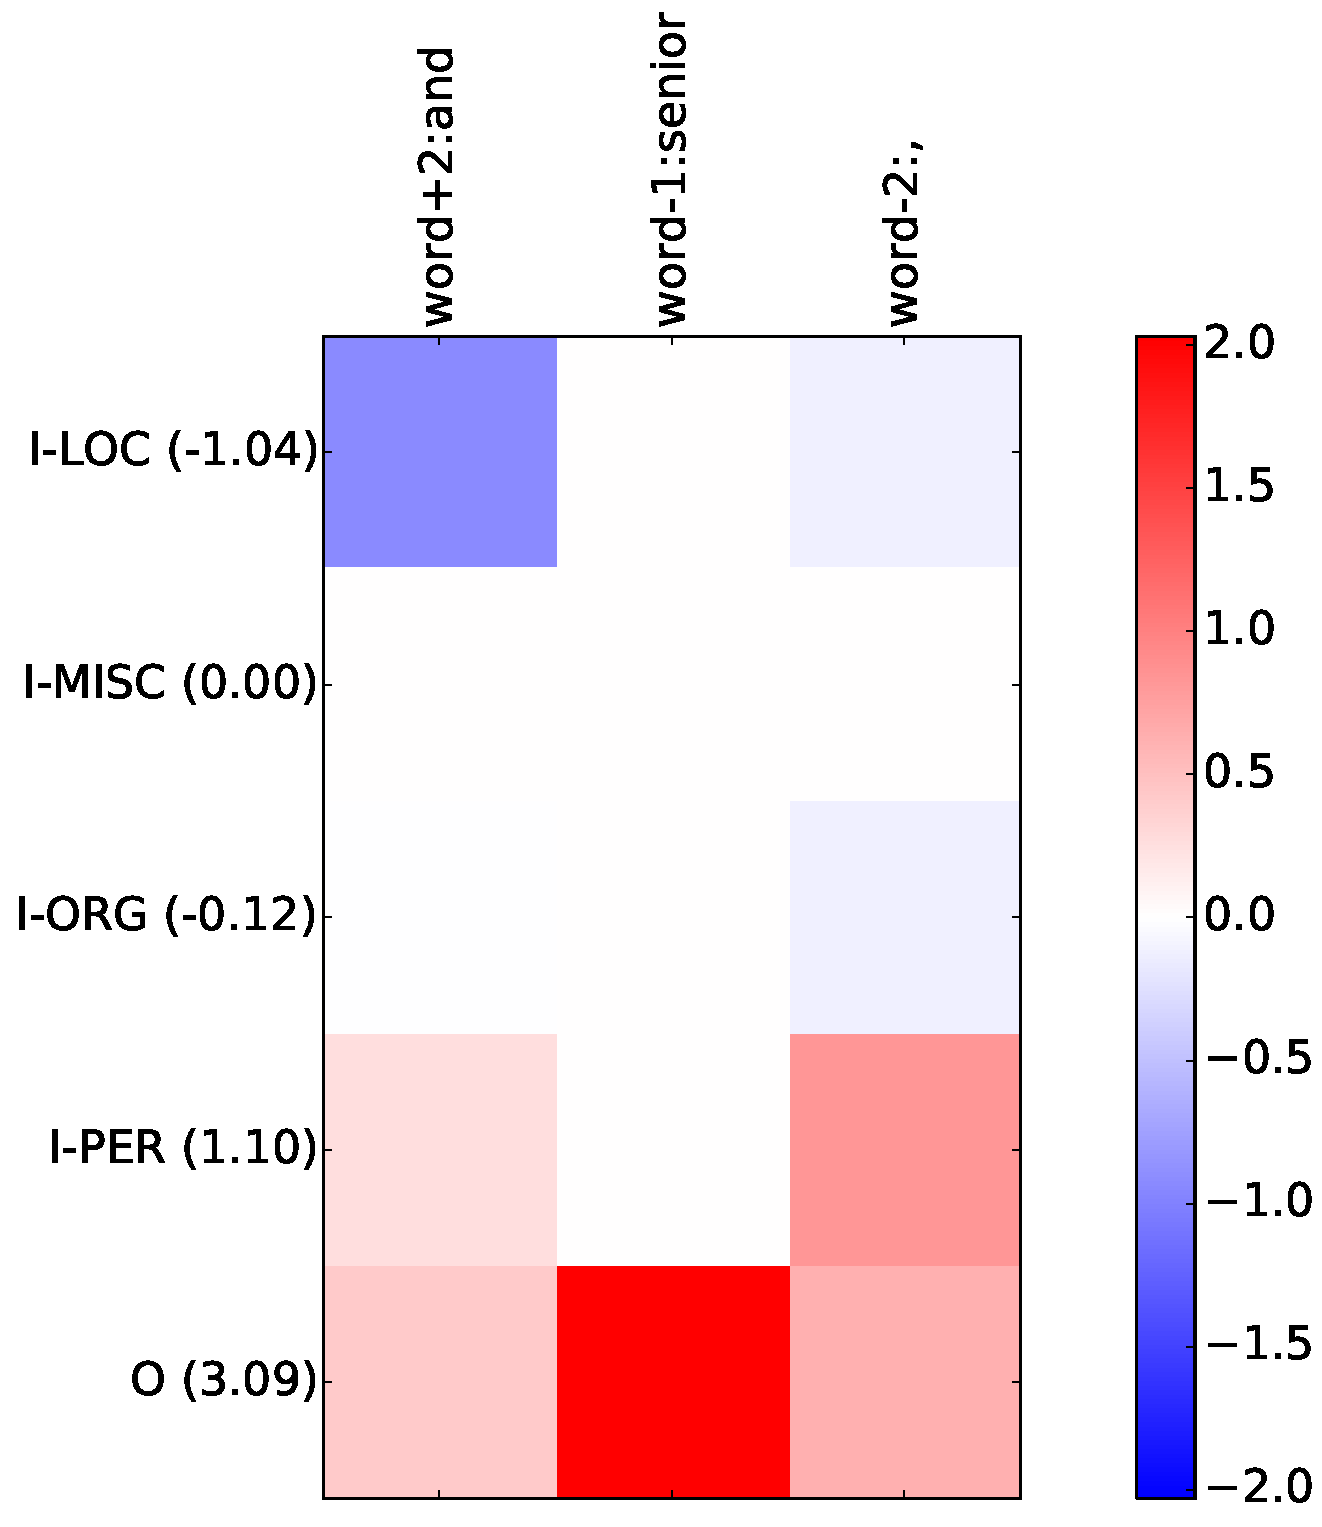
\includegraphics[width=0.9\linewidth]{images/Chapitre4/M1_383.pdf}
	\captionof{figure}{The word \textit{Kory} is predicted to be class O by model $M_1$ given the coefficients of the features indicated.}
	\label{fig:trans_M1}
	\end{subfigure}% 
	\begin{subfigure}[t]{.5\textwidth}
	\centering
	\captionsetup{width=0.7\textwidth}
	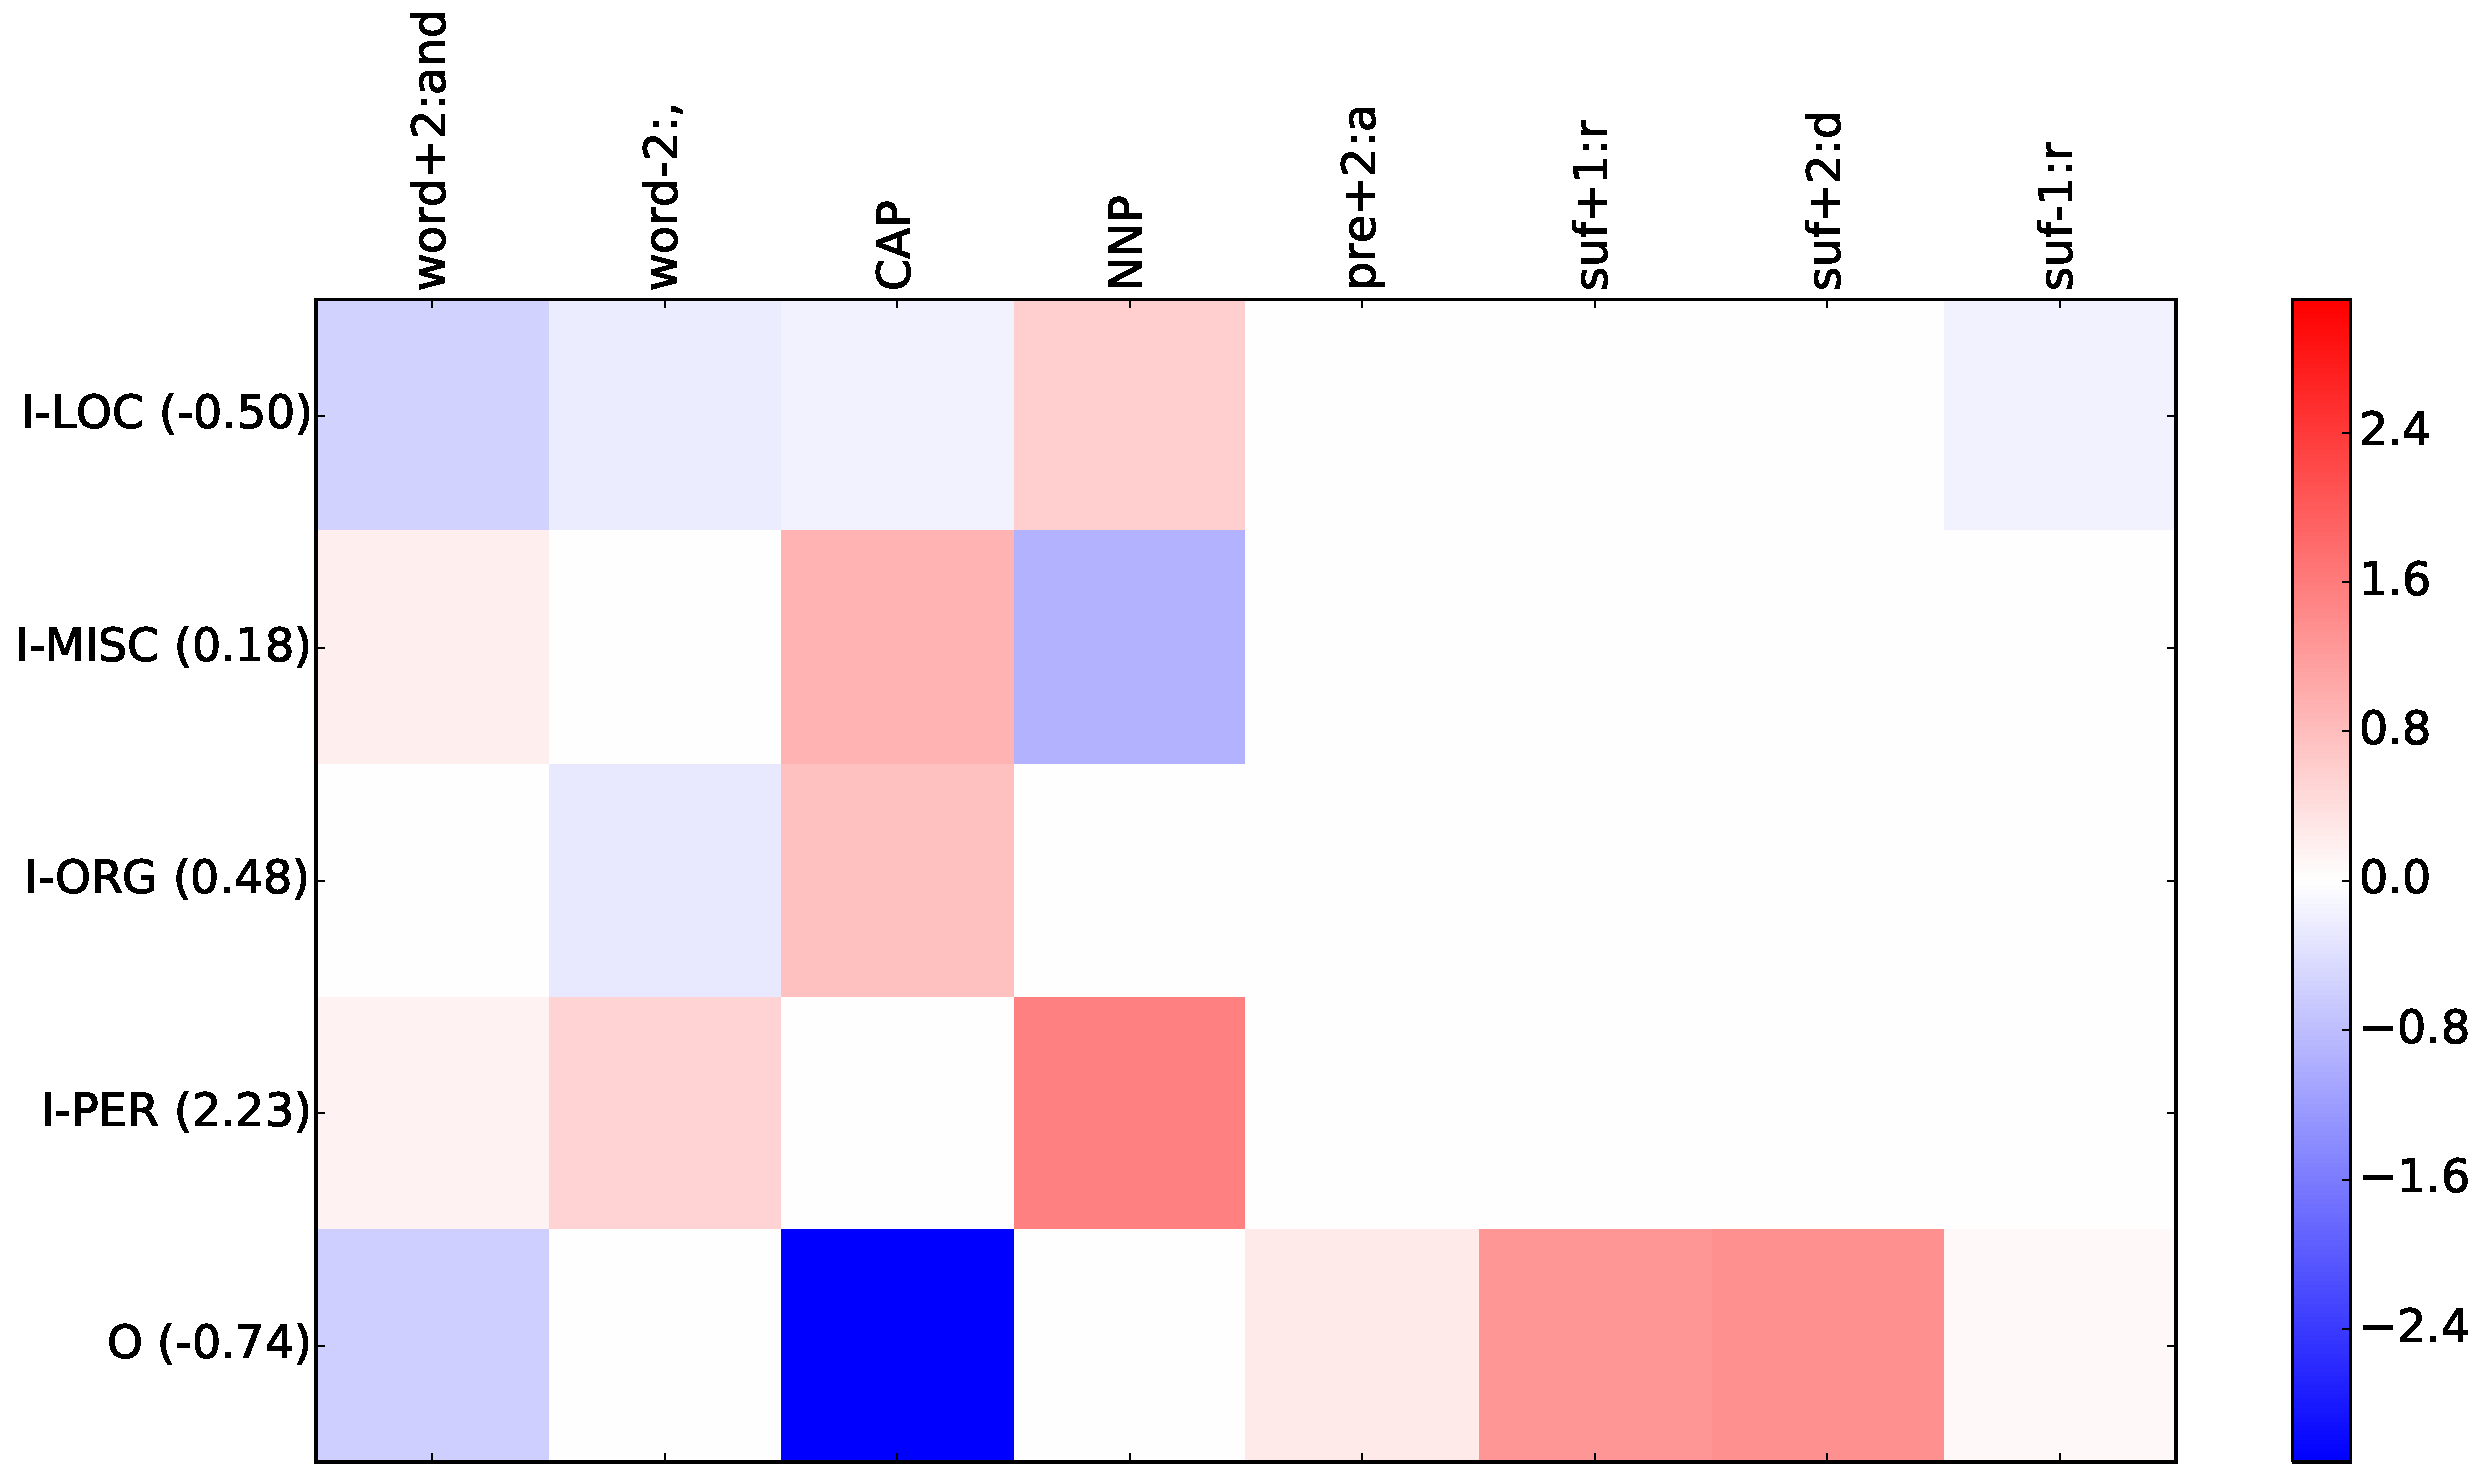
\includegraphics[width=0.9\linewidth]{images/Chapitre4/M2_383.pdf}
	\captionof{figure}{The same word is correctly predicted to be class PER by model $M_2$ given the new features in the model.}
	\label{fig:trans_M2}	
	\end{subfigure}
	\caption{Non-zero coefficients heatmaps for models  $M_1$ and $M_2$ corresponding to the word \textit{Kory}. On the left, $M_1$ fitted using the feature matrix $\mlex$. On the right, model $M_2$ trained using the term $E_{\alpha=0.95}(\mlex, \mstd)$. Red colors are positive, blue are negative. The color intensity varies according to the magnitude of the value.}
	\label{fig:trans_M1_M2}
\end{figure}
\begin{figure}
	\centering
	\begin{subfigure}[t]{.9\textwidth}
	\captionsetup{width=\textwidth}
	\centering
	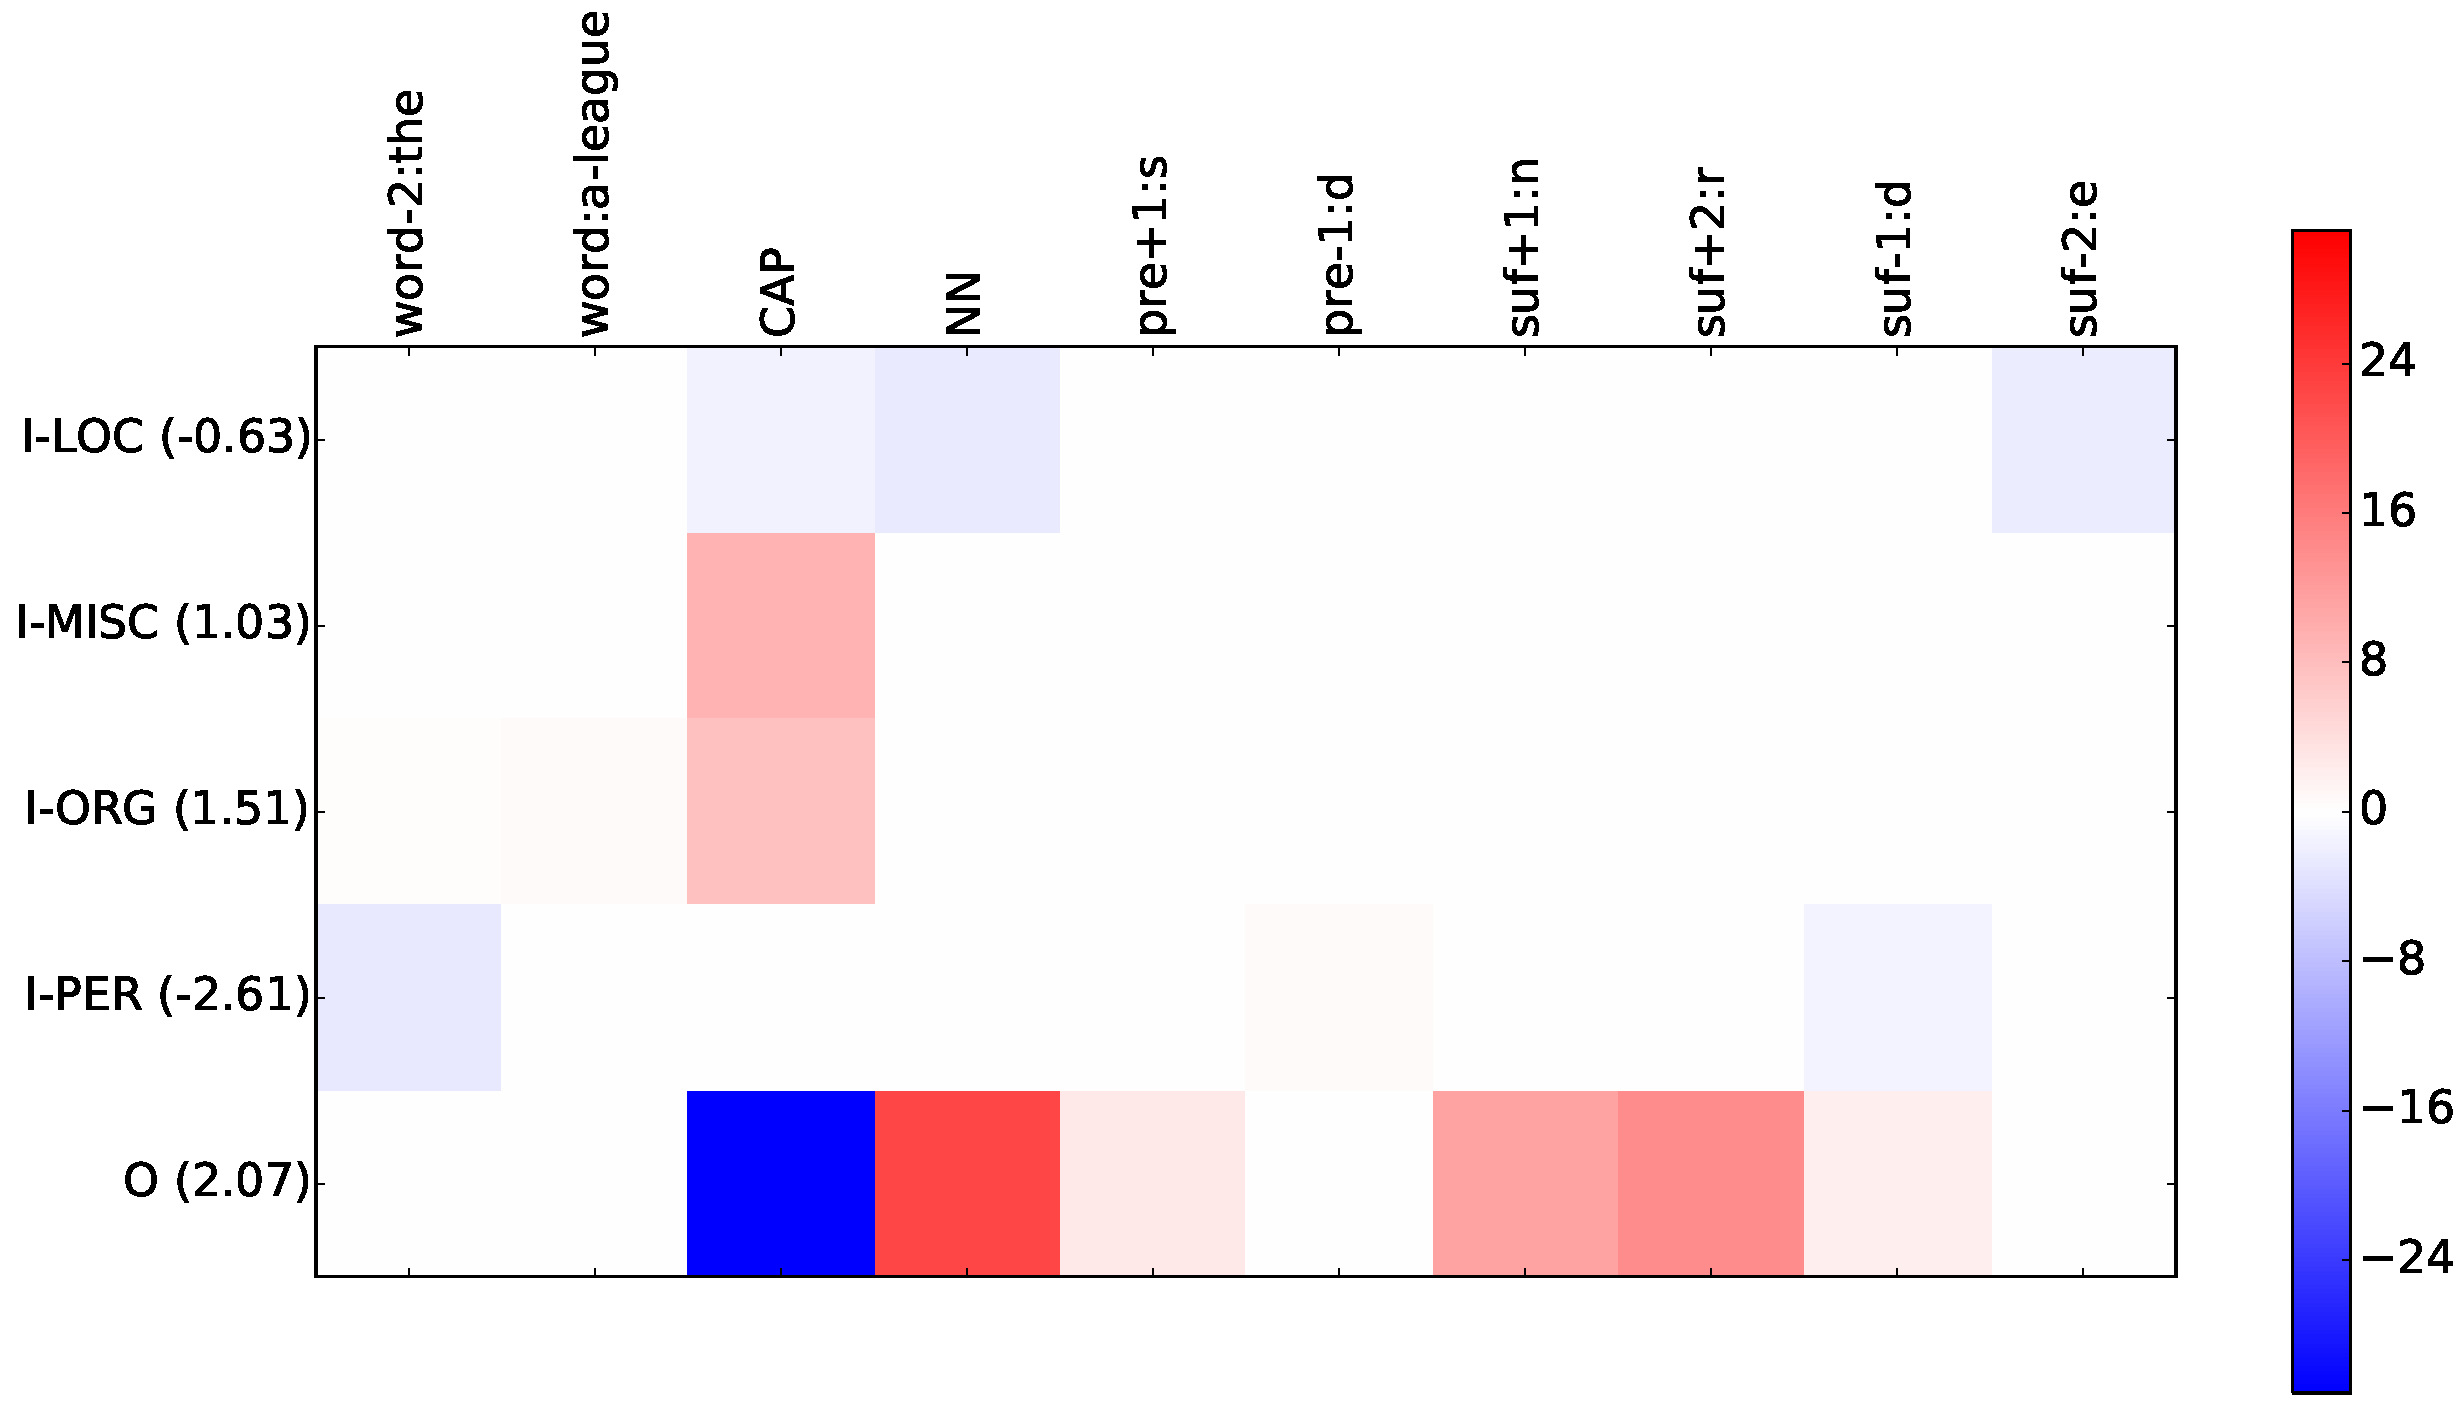
\includegraphics[width=1\linewidth]{images/Chapitre4/M2_1140.pdf}
	\captionof{figure}{The word \textit{A-League} is predicted to be class O by model $M_2$ given the coefficients of the features indicated.}
	\label{fig:trans_M22}
	\end{subfigure}\\%  
	\begin{subfigure}[t]{.9\textwidth}
	\captionsetup{width=\textwidth}
	\centering
	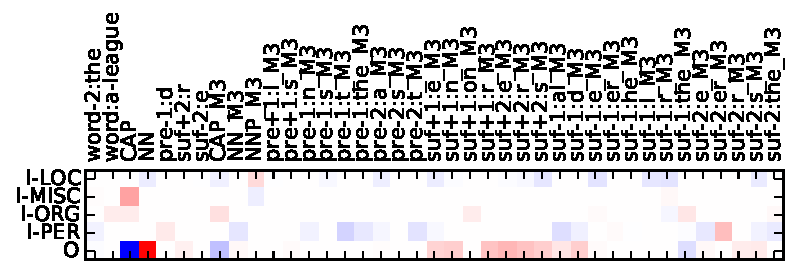
\includegraphics[width=1\linewidth]{images/Chapitre4/M3_1140.pdf}
	\captionof{figure}{The same word is correctly predicted to be class ORG by model $M_3$ given the new features in the model.}
	\label{fig:trans_M3}
	\end{subfigure}
	\caption{Non-zero coefficients heatmaps   for models $M_2$ and $M_3$ corresponding to the word \textit{A-League}. On top, $M_2$ fitted using the term $E_{\alpha=0.95}(\mlex, \mstd)$. On the bottom, model  $M_2$ trained using the  $E_{\alpha=0.95}(\mlex, \mstd, L(\mstd, X_F(\ssyn, \mstd)))$ combination. Red colors are positive, blue are negative. The color intensity varies according to the magnitude of the value.}
	\label{fig:trans_M2_M3}
\end{figure}



\subparagraph{From $\mathbf{M_2}$ to $\mathbf{M_3}$} Going from model ${M_2}$ to ${M_3}$, we focus on the word \textit{A-League}. In the first model, $M_3$ (Figure \ref{fig:trans_M22}), \textit{A-League} is classified as O, since it being a  noun\footnote{The PoS tagger identified it as a simple noun.} (and not a proper noun) seems to be a good indication of a noun not being part of named entity, among other features, such as \textit{suf+2:r}, i.e., the last letter of the second word to the right of \textit{A-League}, in this case \textit{r}. 

With respect to model $M_3$ (see Figure \ref{fig:trans_M3}), \textit{A-League} is correctly tagged as ORG. While the largest coefficients are assigned to the features of the model $M2$ (namely CAP and NN), we can see that the enriched features \textit{CAP\_M3}\footnote{Features added by the third fusion operation are labeled with a \textit{\_M3} suffix. The same is done for the fourth fusion with the suffix \textit{\_M4}} and \textit{suf-1:the\_M3} play a decisive role into the assignation of the class ORG, as most of the values corresponding to the newly added features are positive for this class.



\begin{figure}[h!]
	\centering
	\begin{subfigure}[t]{.9\textwidth}
	\centering
	\captionsetup{width=\textwidth}
	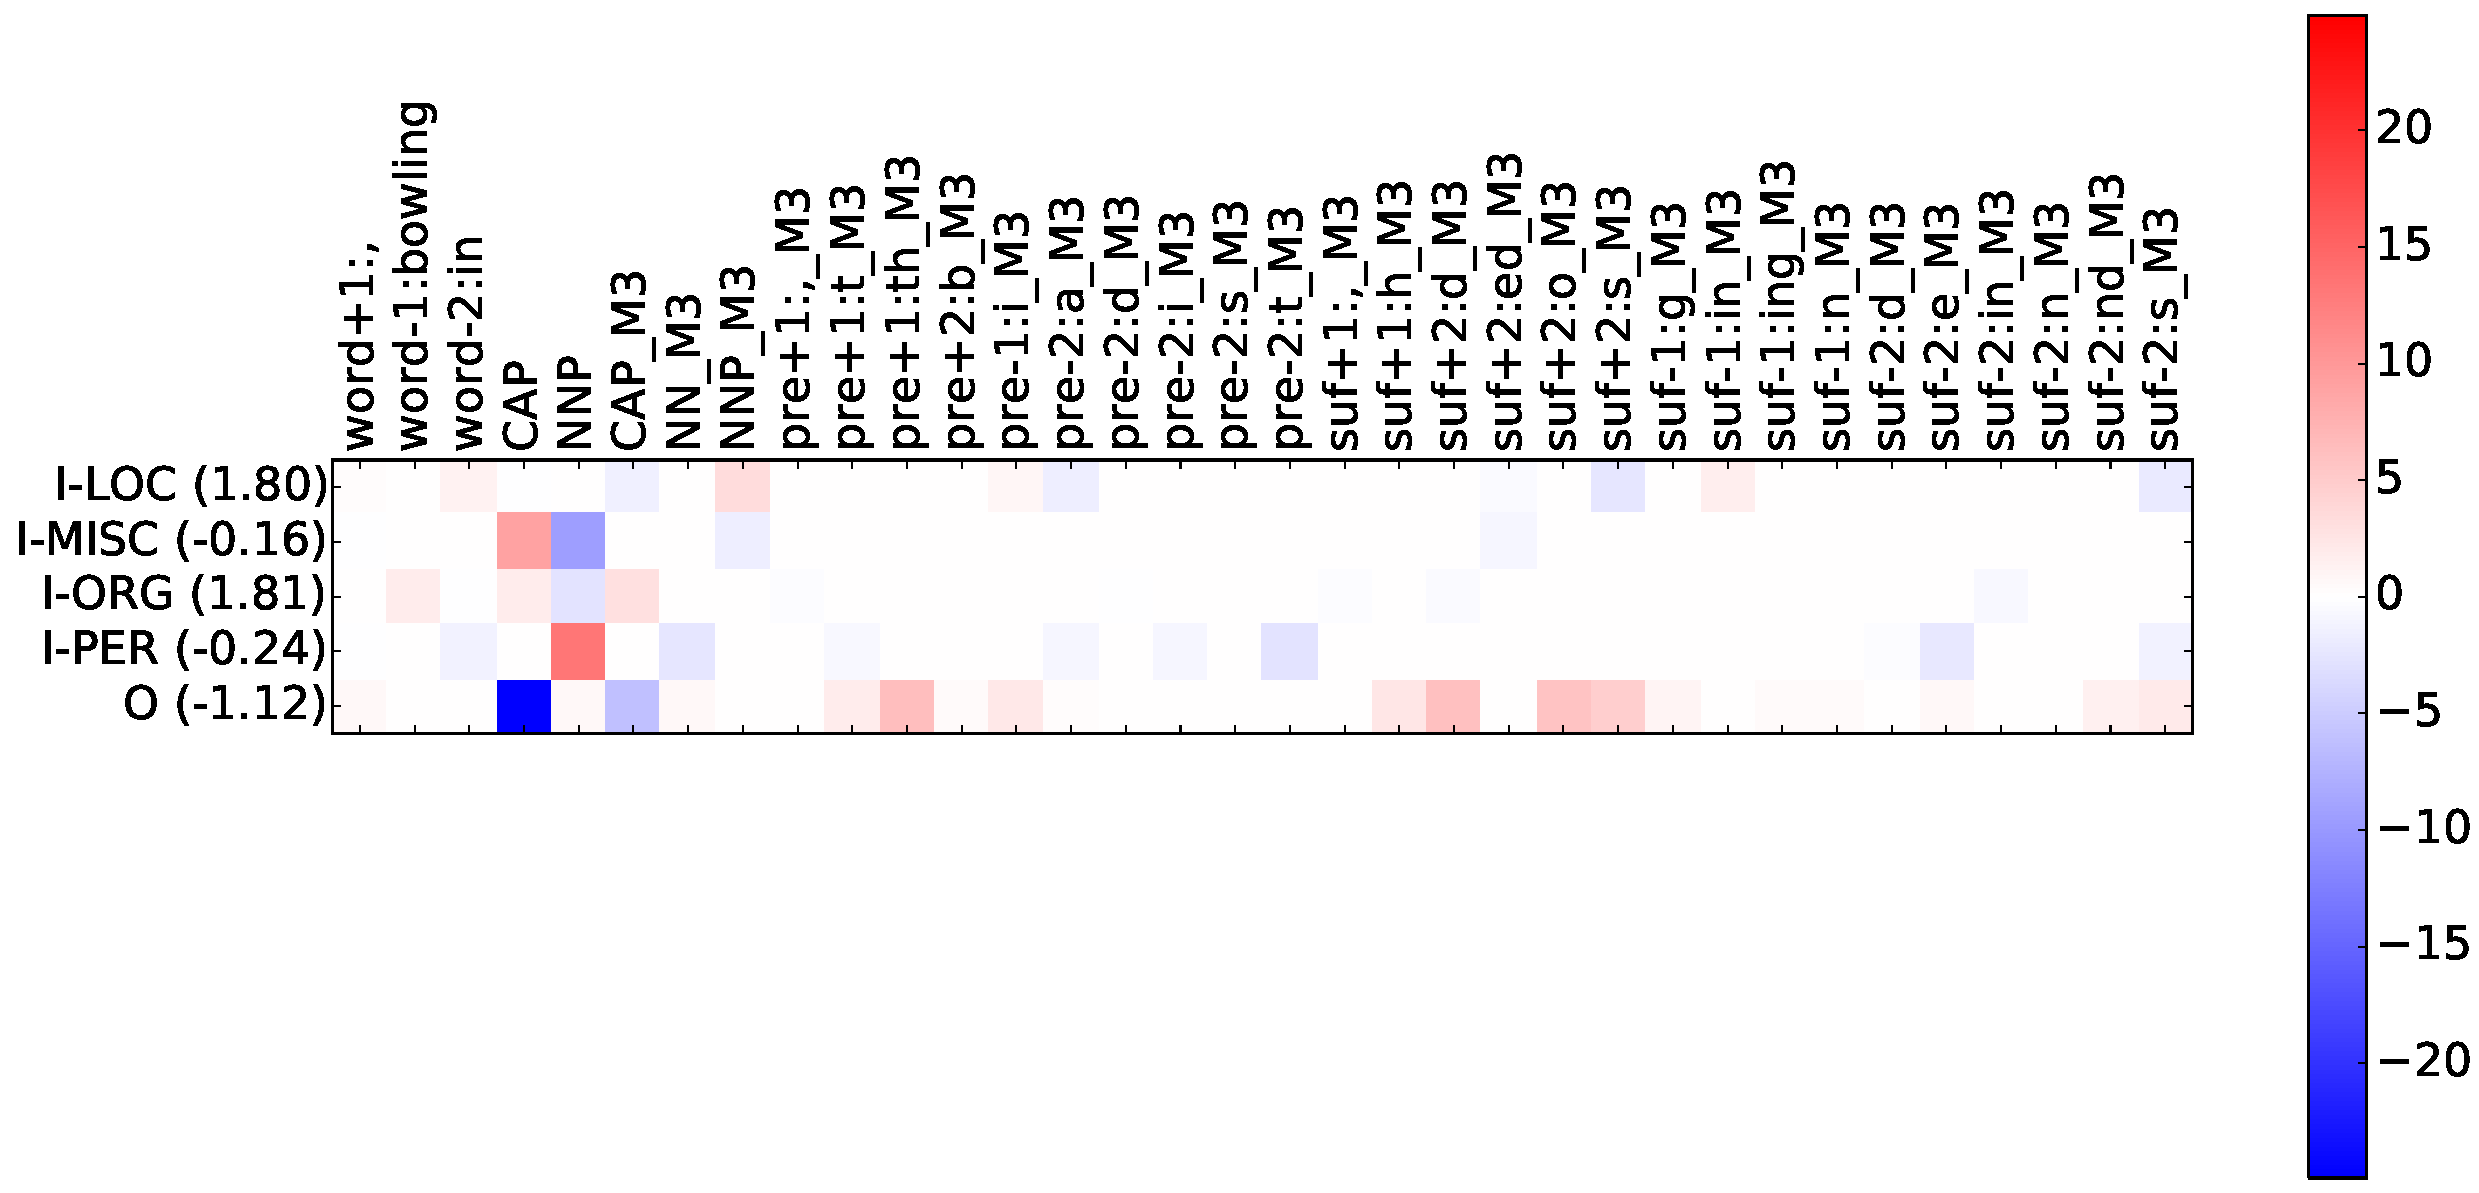
\includegraphics[width=1\linewidth]{images/Chapitre4/M3_16029.pdf}
	\captionof{figure}{The word \textit{Green} is predicted to be class ORG by model $M_3$ given the coefficients of the features indicated.}
	\label{fig:trans_M33}
	\end{subfigure}\\% 
	\begin{subfigure}[t]{.9\textwidth}
	\centering
	\captionsetup{width=\textwidth}	
	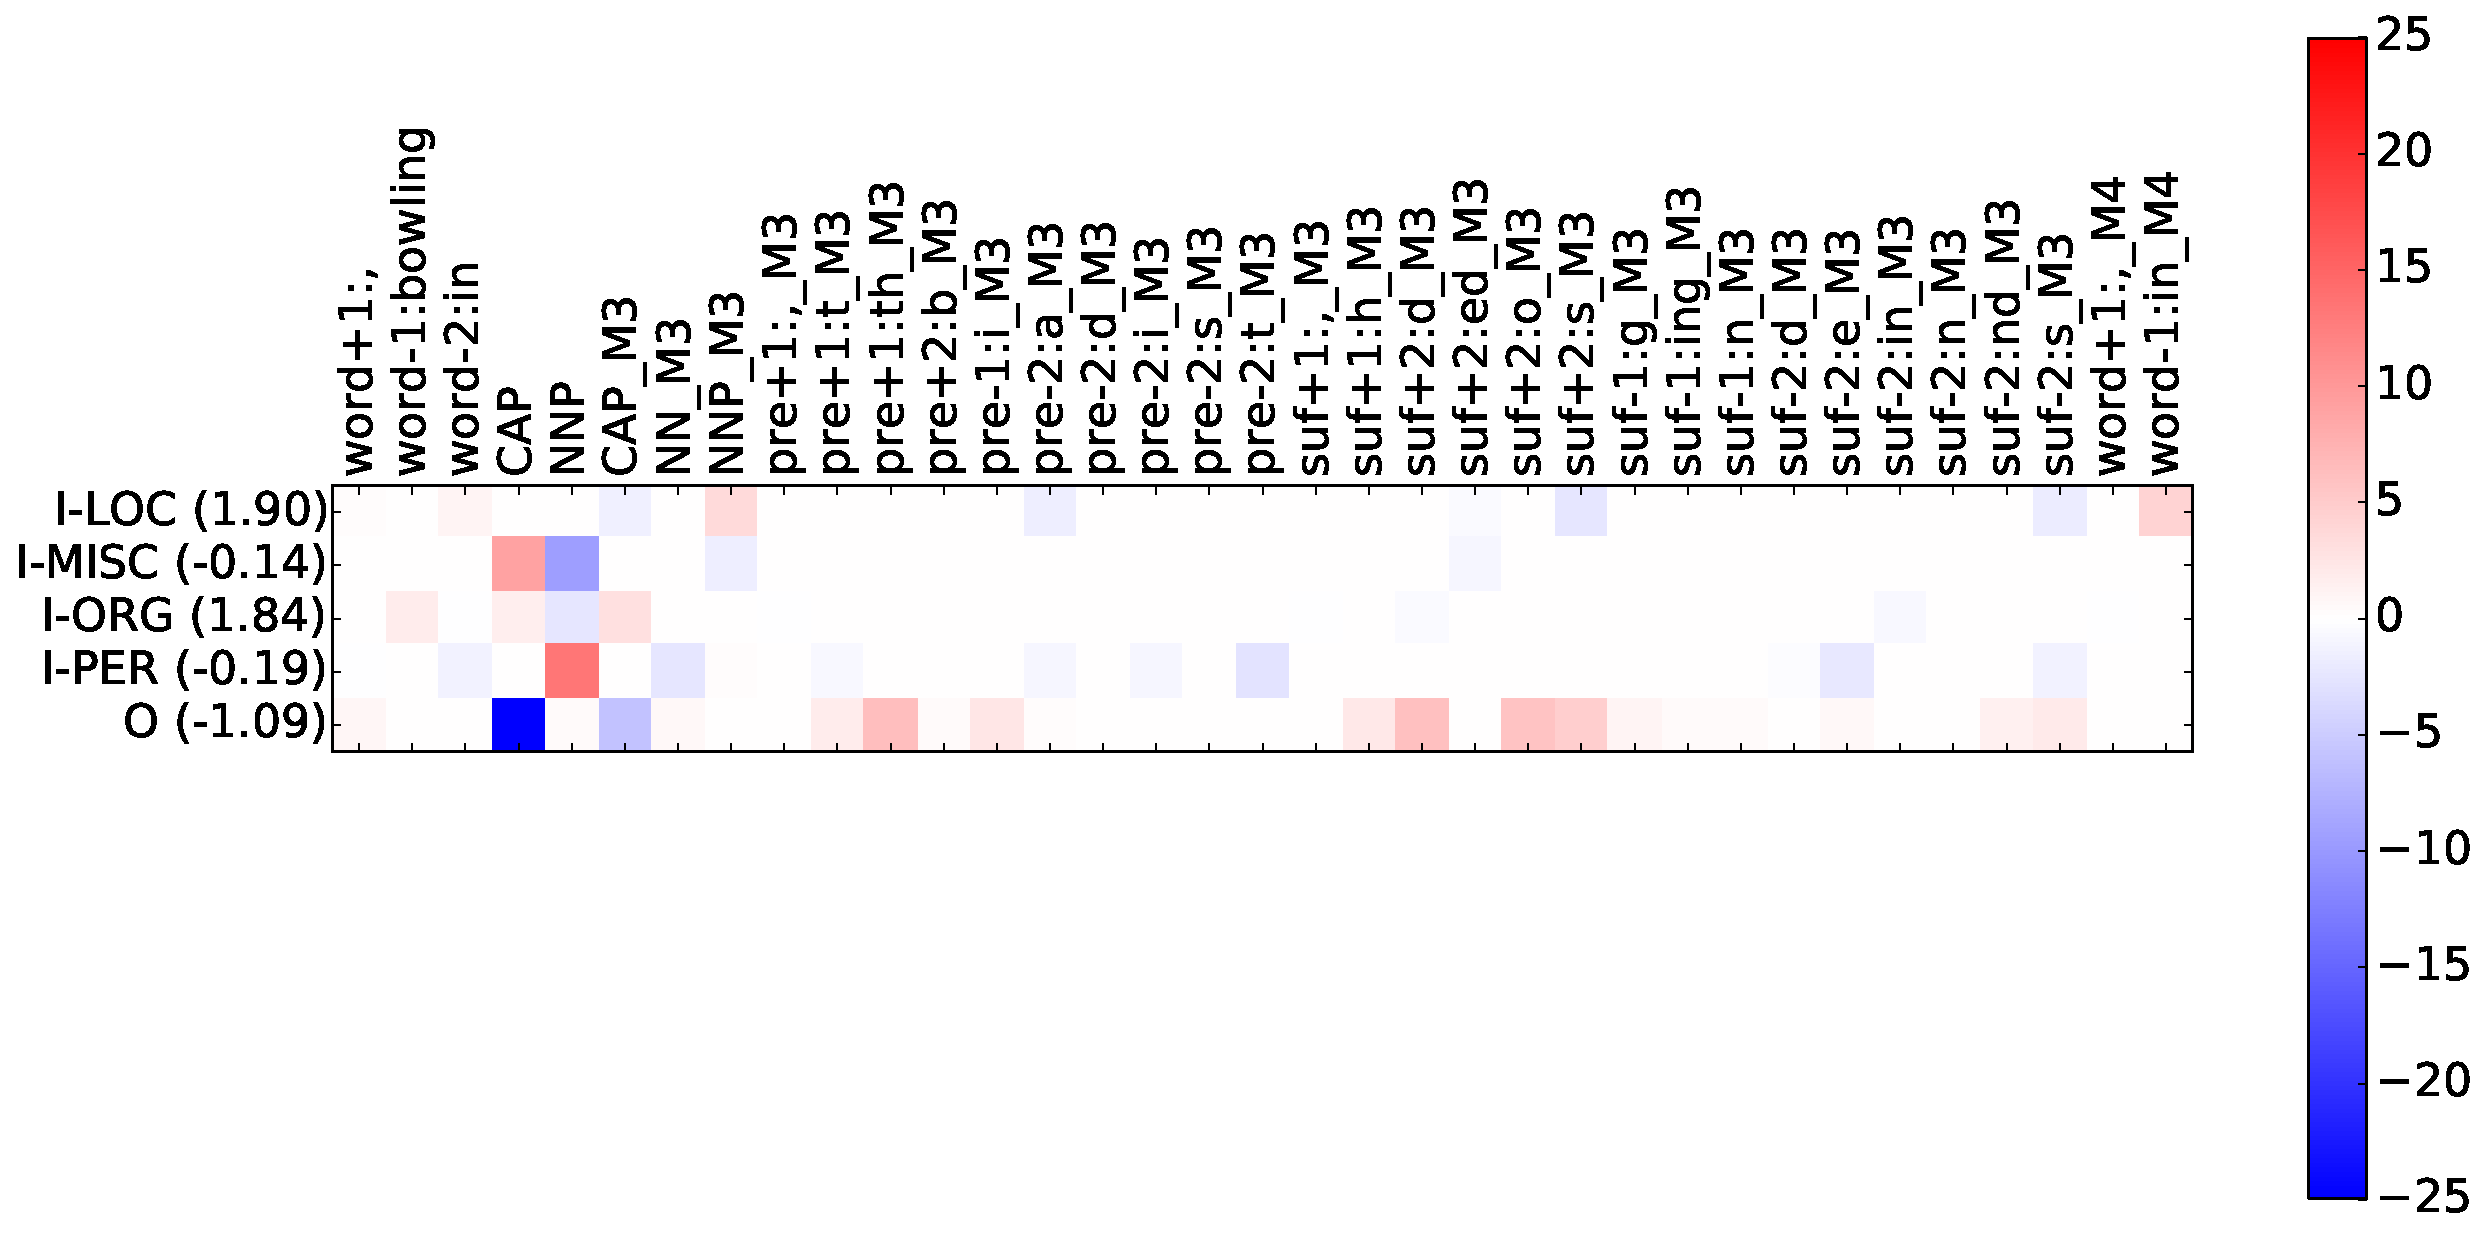
\includegraphics[width=1\linewidth]{images/Chapitre4/M4_16029.pdf}
	\captionof{figure}{The same word is correctly predicted to be class LOC by model $M_4$ given the new features in the model.}
	\label{fig:trans_M4}
	\end{subfigure}
	\caption{Non-zero coefficients heatmaps for  models $M_3$ and $M_4$ corresponding to the word \textit{Green}. On top, $M_3$ fitted using the term $E_{\alpha=0.95}(\mlex, \mstd, L(\mstd, X_F(\ssyn, \mstd)))$. On the bottom, model $M_4$ trained using   $E_{\alpha=0.95}(\mlex, \mstd, L(\mstd, X_F(\ssyn, \mstd)), L(\mlex, X_F(\ssyn, \mlex)))$ as fusion operator. Red colors are positive, blue are negative. The color intensity varies according to the magnitude of the value.}
	\label{fig:trans_M3_M4}
\end{figure}

\subparagraph{From $\mathbf{M_3}$ to $\mathbf{M_4}$} Finally, going from model $M_3 $ to model $M_4$, in Figure \ref{fig:trans_M3_M4} we have an incorrect ORG classification to a correct LOC classification after the application of the last fusion operation. The chosen word is \textit{Green}. Both coefficients' values are quite similar  to each other (see Figures \ref{fig:trans_M33} and \ref{fig:trans_M4}). In fact, the score in parentheses for both LOC and ORG are quite close in both models. This is expected as their difference in performance is small (see Table \ref{tab:4ops}). Not surprisingly, there are only two features coming from the last fusion (the last two columns, indicated with a \textit{\_M4} suffix. Nonetheless, it seems that one of these enriched features, \textit{word-1:in\_M4} determines the model decision towards the LOC class, thus making the correct classification.

In general, in these experiments, we see that the added enriched features are not the highest valued in the fitted coefficients vectors, nonetheless, they  provide the extra information needed to push the model towards the correct prediction, by enriching the features through cross and late fusion and by providing more descriptors for each word and consequently reducing the sparsity of the representation matrices.

Once we found a set of fusion operations that work reasonably well with NER, we experiment with another task, word sense induction and disambiguation, to confirm the usefulness of using fusion enriched representations to train better models.

In the next subsection we present a series of analogous experiments, this time solving WSI/WSD.


\section{Second Application: Word Sense Induction and Disambiguation}
\label{sec:wsd_wsi}
Word Sense Induction and Disambiguation entails two closely related tasks\footnote{Even though these tasks are closely related, they are independent from one another. Still,  we consider them to be a single one: WSI/WSD.}. WSI aims to automatically discover the set of possible senses for a target word given a text corpus containing several occurrences of said target word. Meanwhile, WSD takes a set of possible senses and determines the most appropriate sense for each instance of the target word according to the instance's context. WSI is usually approached as an unsupervised learning task, i.e., a cluster method is applied to the words occurring in the instances of a target word. The groups found are interpreted as the senses of the target word. The WSD task is usually solved with knowledge-based approaches, based on WordNet; or more recently with supervised models which require annotated data. It can be also solved reasonably well by comparing the words surrounding each target word and the words belonging to the induced senses (or clusters) found during the WSI step.

We believe that in order to solve WSD in a truly end-to-end unsupervised way, one would need to first automatically find a list of senses for a word without the help of pre-built semantic networks. In other words, solve WSI. Word sense induction is usually solved as follows:

Given an input document with a set of target words, coupled with a set of contexts (a target word in a unique context is called an instance), the goal is to discover a list of senses for each target word and then assign each instance in the document with an automatically generated sense (this part corresponds to WSD). The common four steps used are the following:

\begin{enumerate}
\item Build a lexical co-occurrence network (LCN), or similar, assigning tokens as nodes and  establishing edges between them if they co-occur in a given context (usually if they both appear in the same sentence, paragraph or fixed window of words).
\item Determine the weights for each edge either according to a frequency metric or using binary weights. 
\item Apply a graph clustering algorithm. Each cluster found will represent a sense of the polysemous target word.
\item Match target word instances with the clusters found (the senses) by using the word context. Specifically, assign a sense to each instance by looking at the tokens in the context. This step is actually the word sense disambiguation task. 
\end{enumerate}	


Word sense induction, while being an unsupervised and thus more flexible task (language and word-domain independent, does not require human-made knowledge bases), require a good quality clustering algorithm, as its results are tightly linked to its performance.
\subsection{Fusion Enriched Representations}

In this subsection we also employ the hypergraph model introduced before to propose a solution to both WSD and WSI tasks, specifically the enrichment of features via fusion techniques.

The WSI method, i.e., the clustering algorithm, we employ is not original, as we will see. Nonetheless, our interest lies on  using a combined representation, which is able to address certain concerns that are not deeply studied, namely the use of heterogeneous context features to solve semantic tasks while reducing the number of parameters compared to similar approaches.  Our method is evaluated with a corpus corresponding to the WSI task of the international workshop of semantic evaluations, edition 2007, or Semeval 2007. 

As shown in Figure \ref{fig:diagmetodoWSD}, the procedure we follow is very similar to that of the previous NER experiments. The difference being the task addressed and the features employed (we find clusters using only lexical and syntactic contexts).
\begin{figure}[t]
\centering
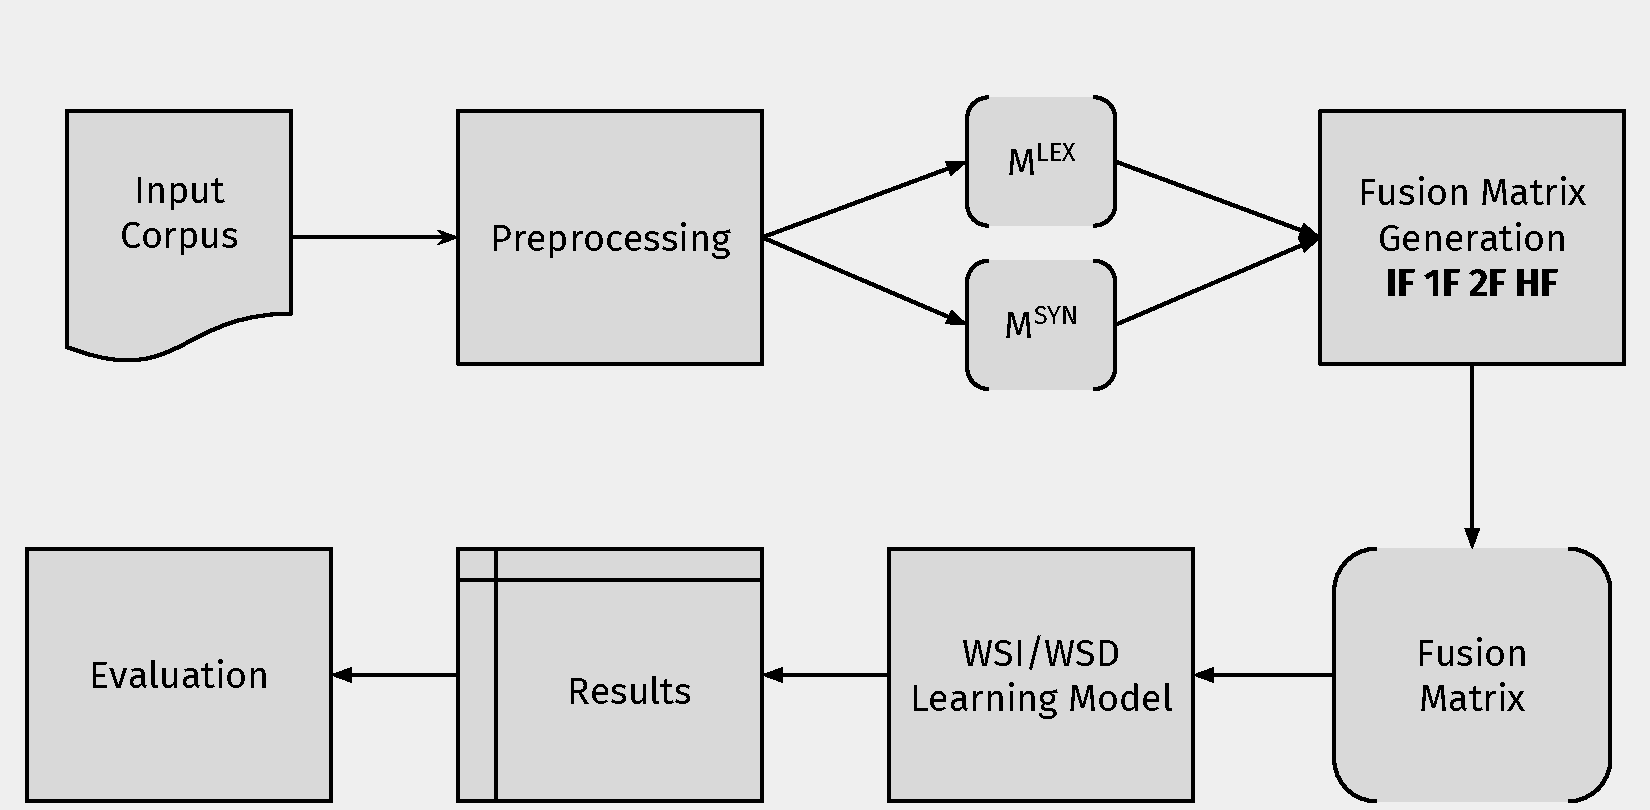
\includegraphics[width=0.85\linewidth]{images/Chapitre4/diag_metodoWSD.pdf}
\caption{Steps followed on our fusion-enriched representation for WSI/WSD experiments. First the corpus is lightly preprocessed, then features are extracted from the text. A fusion matrix is generated, which in turn is used as input to the learning algorithm. Finally, the system yields its results and to be analyzed.}
\label{fig:diagmetodoWSD}
\end{figure}
%\subsection{Introduction}



We discovered a set of successful fusion operations in the previous experiments. In these experiments we set to test if the improvements obtained before, using said fusion schemes, can be transferred into WSI/WSD and other corpora. 

\paragraph{Representation Spaces}
We use the same set of features from the previous subsection (see \ref{sec:rep_spaces}), except for the standard NER features, that is, those represented by $\mstd$, as they are specifically designed to tackle that task. Consequently, we will experiment with two representation matrices $\mlex$ and $\msyn$.

\paragraph{Learning Methods}
Regarding the machine learning methods to induce senses, (the WSI part), we employ spectral clustering (as is described previously in Chapter 3, paragraph \ref{par:partitioning_clustering}) on the input matrices in order to automatically discover senses (a cluster is considered a sense). As we noted before, this method require as input a symmetric positive similarity matrix. Given that our fusion operators already may yield similarity matrices (e.g., late fusion of similarity matrices). If that is the case, we use this type of matrix directly as input to the algorithm. Otherwise, we compute the cosine similarity to obtain the corresponding affinity matrix and then use it as input. Similarly, spectral clustering is said to be more efficient if the input matrix is sparse \cite{song2008parallel}. We do not sparsify the matrix, usually done by applying a top-$k$ nearest neighbors selection, as we already apply said selection in certain fusion operators and it then becomes even harder to track the modifications applied to the feature space.

 Regarding disambiguation, we trivially assign senses to the target word instances according to the number of common words in each cluster and the context words of the target word. In other words, for each test instance of a target word, we select the cluster (sense) with the maximum number of shared words with the current instance context.

\paragraph{Experiments and Evaluation}
Having learned the best fusion configuration from the previous task, in these experiments we set to test if the improvements achieved can be transfered into another NLP task, namely Word Sensed Induction and Disambiguation (WSI/WSD). As preprocessing, we simply remove stopwords and tokens with less than three letters. The features we extracted from the tested corpora with the same tools as in the previous task.
\subparagraph{Test Dataset}
The WSI/WSD model is tested on the dataset of  the Semeval 2007 WSID task \cite{Agirre2007}. The task was based on a set of 100 target words (65 verbs and 35 nouns), each  word having a set of instances, which are specific contexts where the word appear. Senses are induced from these contexts and applied to each one of the instances.

%In the case of Semeval 2007, the unsupervised evaluation assumed the induced senses as clusters of examples. These clusters are compared to the sets of examples tagged with the given gold standard word senses (classes), and evaluated using the \textit{F-measure} measure for clusters. 
% 
%The supervised setting maps the induced senses to manually-defined gold standard senses, and use a mapping produced by the organizers to tag the test corpus with gold standard tags. The mapping is
%automatically produced by the organizers, and the resulting results evaluated according to the
%usual precision and recall measures for supervised word sense disambiguation systems. 


\subparagraph{Evaluation Measures}
Being an unsupervised task, the evaluation metrics of WSI/WSD are debated in terms of quality \cite{CruysA11}. We consider supervised recall and unsupervised F-measure, as in the competition original paper \cite{Agirre2007}. The first one maps the output of a system to the true senses of the target words' instances and the second one measures the quality of the correspondence between the automatically found clusters and the senses. 
We consider that the number of senses found by the system is also a rather good indicator of performance: the best competition baseline assigns the most frequent sense to each target word (this baseline is called the Most Frequent Sense or MFS), thus this baseline system would have an average of 1 sense (cluster) per word. A system that goes near this average may be indeed not resolving the task efficiently but finding the MFS trivial solution. Consequently, to show that we do not fall in the MFS solution, we display in our results the average number of clusters.




\begin{table}[htp!]
\centering
%\setlength\tabcolsep{3pt}
\caption{All-words, nouns, and verbs supervised recall for the Semeval 2007 corpus using fusion operations (SF, 1F, 2F, HF) and spectral clustering. We also display the average number of clusters found by each fusion configuration, the best performing system as well as the MFS baseline. In bold the best results per-column among our experiments.}
\label{tab:wsd-semeval_sup_Recall}
\begin{tabular}{@{}lrrrrc@{}}
\toprule
\textbf{Fusion Operation / System} & \multicolumn{3}{c}{\textbf{Recall (\%)}} & \#\textbf{cl} & \textbf{Fusion Level}\\ 
        & \textbf{all}          & \textbf{nouns}          & \textbf{verbs} &          \\ 
       \midrule
        \multicolumn{5}{r}{\textbf{Single Features}} & \multirow{3}{*}{\textbf{SF}} \\ %\midrule
       $\mlex$                    & 79.20 & 82.10 & 75.80 & 4.13\\
 

       $\msyn$                    & 79.10 & 81.60 & \textbf{76.20} & 4.47\\
       \midrule
                   \multicolumn{5}{r}{\textbf{Early Fusion (EF)}}  & \multirow{10}{*}{\textbf{1F}}     \\ %\midrule
       $E(\mlex, \msyn)$		& 78.70 & 81.11 & 76.10 & 4.46\\
	  %\midrule
                   \multicolumn{5}{r}{\textbf{Cross Feature Fusion ($\mathbf{X_FF}$)}}       \\ %\midrule	         
	   
	   $X_F(\slex, \mlex)$		& 79.20 & 82.30 & 75.70  & 3.63\\	   
       $X_F(\slex, \msyn)$		& 78.30 & 80.90 & 75.30  & 3.08\\
	   $X_F(\ssyn, \mlex)$		& 78.60 & 80.90 & 76.10  & 1.08\\	   
       $X_F(\ssyn, \msyn)$		& 78.90 & 81.40 & 76.10 & 2.72\\       
 %\midrule
                   \multicolumn{5}{r}{\textbf{Cross Similarity Fusion ($\mathbf{X_SF}$)}}       \\ %\midrule
	   
 
	   $X_S(\ssyn, \slex)$		& 78.70 & 80.90 & \textbf{76.20}  & 1.01\\
	   $X_S(\slex, \ssyn)$		& 78.80 & 80.90	& 76.06 & 1.33\\
	  
 \midrule
                   \multicolumn{5}{r}{\textbf{Cross Feature Cross Similarity Fusion ($\mathbf{X_FX_SF}$)}}  & \multirow{9}{*}{\textbf{2F}}     \\ %\midrule
	   
       $X_F(X_S(\slex, \ssyn), \mlex)$		& 78.40 & 80.40 & 76.10 & 3.11 \\	   
       $X_F(X_S(\slex, \ssyn), \msyn)$		& 78.90 & 81.80 & 75.60 & 3.16\\	   
       	  %\midrule
                   \multicolumn{5}{r}{\textbf{Early Cross Feature Fusion ($\mathbf{EX_FF}$)}}       \\ %\midrule	         
       
       $E(\mlex, X_F(\slex, \mlex))$		& 79.20 & 82.40 & 75.70 & 3.57\\	   
	   $E(\msyn, X_F(\slex, \mlex))$		& 78.30 & 80.50 & 75.80 & 1.95\\	   
       %\midrule
                   \multicolumn{5}{r}{\textbf{Late Cross Feature Fusion ($\mathbf{LX_FF}$)}}       \\ %\midrule	  
	   $L(\msyn, X_F(\slex, \msyn))$		& 78.60 & 81.10 & 75.80 & 4.22\\	   
	   $L(\mlex, X_F(\slex, \mlex))$		& \textbf{79.50} & \textbf{82.80} & 75.70 & 3.96\\	   
       \midrule
                   \multicolumn{5}{r}{\textbf{Early Late Cross Feature Fusion ($\mathbf{ELX_FF}$)}}     & \multirow{3}{*}{\textbf{HF}}  \\ %\midrule	  
	   $E(\mlex, L(\msyn, X_F(\slex, \msyn)))$		& 78.50 & 81.40 & 75.40 & 4.26\\	   
	   $E(\mlex, L(\mlex, X_F(\slex, \mlex)))$		& \textbf{79.50} & 82.70 & 75.90 & 3.99\\
	   \midrule
	   \midrule
	   

	   Baseline MFS		& 78.70 & 80.90 & 76.20 & 1.00\\ 	   	 	    
	   Semeval 2007 Best System& 81.60 & 86.80 & 75.70 & 1.15\\ 	 		   
       \bottomrule
\end{tabular}
\end{table}


\begin{table}[htp!]
\centering
\setlength\tabcolsep{3pt}
\caption{All-words, nouns, and verbs unsupervised F-measure for the Semeval 2007 corpus using fusion operations (SF, 1F, 2F, HF) and spectral clustering. We also display the average number of clusters found by each fusion configuration, the best performing system as well as the MFS baseline. In bold the best results per-column among our experiments.}
\label{tab:wsd-semeval_unsup_fm}
\begin{tabular}{@{}lrrrrc@{}}
\toprule
\textbf{Fusion Operation / System} & \multicolumn{3}{c}{\textbf{F-measure (\%)}} & \#\textbf{cl} & \textbf{Fusion Level}\\ \midrule
      	& \textbf{all}          & \textbf{nouns}          & \textbf{verbs}           \\ 
       \midrule
       \multicolumn{5}{r}{\textbf{Single Features}} & \multirow{3}{*}{\textbf{SF}}\\ %\midrule
       $\mlex$                    &	72.70	 & 76.90 & 67.90 & 4.13\\
 

       $\msyn$                    &	69.30	& 69.40 & 69.20 & 4.47\\
       \midrule
       \multicolumn{5}{r}{\textbf{Early Fusion (EF)}}  & \multirow{10}{*}{\textbf{1F}}     \\ %\midrule
       $E(\mlex, \msyn)$		&	74.00	& 76.66 & 71.11 & 4.46\\
	  %\midrule
       \multicolumn{5}{r}{\textbf{Cross Feature Fusion ($\mathbf{X_FF}$)}}       \\ %\midrule	         
	   
	   $X_F(\slex, \mlex)$		&	76.20	& 79.60 & 72.50 & 3.63 \\	   
       $X_F(\slex, \msyn)$		&	74.60	& 75.10 & 73.90 & 3.08 \\
	   $X_F(\ssyn, \mlex)$		&	\textbf{78.90}	& 80.70 & \textbf{76.90}	 & 1.08 \\	   
       $X_F(\ssyn, \msyn)$		&	73.70	& 77.70 & 70.00 & 2.72 \\       
% \midrule
       \multicolumn{5}{r}{\textbf{Cross Similarity Fusion ($\mathbf{X_SF}$)}}       \\ %\midrule
	   
 
	   $X_S(\ssyn, \slex)$		&	\textbf{78.90}	& \textbf{80.80} & 76.80 & 1.01 \\
	   $X_S(\slex, \ssyn)$		&	78.70	& 80.50  & 76.80 & 1.33 \\
	  
 \midrule
       \multicolumn{5}{r}{\textbf{Cross Feature Cross Similarity Fusion ($\mathbf{X_FX_SF}$)}}   & \multirow{9}{*}{\textbf{2F}}    \\ %\midrule

       $X_F(X_S(\slex, \ssyn), \mlex)$		&	70.00	&68.70  & 71.40& 3.11 \\	   
       $X_F(X_S(\slex, \ssyn), \msyn)$		&	75.20	& 77.40 & 72.80 & 3.16 \\	   
       	  %\midrule
       \multicolumn{5}{r}{\textbf{Early Cross Feature Fusion ($\mathbf{EX_FF}$)}}       \\ %\midrule	         
       
       $E(\mlex, X_F(\slex, \mlex))$		&	76.00	& 79.50  & 72.10 & 3.57 \\	   
	   $E(\msyn, X_F(\slex, \mlex))$		&	75.20	&75.40  & 75.00 & 1.95 \\	   
       %\midrule
       \multicolumn{5}{r}{\textbf{Late Cross Feature Fusion ($\mathbf{LX_FF}$)}}       \\ %\midrule	  
	   $L(\msyn, X_F(\slex, \msyn))$		&	67.80	& 71.40&63.80 & 4.22 \\	   
	   $L(\mlex, X_F(\slex, \mlex))$		&	76.09	&79.10 &72.70 & 3.96 \\	   
       \midrule
       \multicolumn{5}{r}{\textbf{Early Late Cross Feature Fusion ($\mathbf{ELX_FF	}$)}}    & \multirow{3}{*}{\textbf{HF}}   \\ %\midrule	  
	   $E(\mlex, L(\msyn, X_F(\slex, \msyn)))$		&	74.20	& 78.20 & 69.80& 4.26 \\	   
	   $E(\mlex, L(\mlex, X_F(\slex, \mlex)))$		&	75.80	& 78.50&72.70 & 3.99 \\
	   \midrule
	   \midrule
	   Baseline 1c1word 		&	78.90	& 80.70&76.80 & 1.00 \\ 	   	 	    	   
	   Semeval 2007 Best Systems	&	78.70	& 80.80&76.30 & 3.06 \\ 	 

		   
       \bottomrule
\end{tabular}
\end{table}




\paragraph{Results and Discussion}
Word sense induction and disambiguation results, using fusion enriched matrices with spectral clustering, are found in Tables \ref{tab:wsd-semeval_sup_Recall} and \ref{tab:wsd-semeval_unsup_fm} for the supervised recall and unsupervised F-measure respectively.

In the unsupervised evaluation results, we include an interesting baseline which had also the best performing results. The baseline consists in assigning one cluster per word (or {1c1word}), i.e., it simply assigns a single sense to all the test instances of a word. This baseline was not beat during the competition. On the other had, for the supervised results, we include the Most Frequent Sense (or MFS) baseline which tags every test instance with the sense that occurred most often in the training corpus of the competition. Besides these baselines, we included also the best performing systems' results for both of the evaluations.


We experimentally set $\beta=0.90$ and $\gamma=50$. Remember that $\beta$ controls the relevance of each matrix in the late fusion binary operator $L(\beta\cdot A, (1-\beta)\cdot B)$ and $\gamma$ control number of nearest neighbors to take from the first operand of the cross fusion $\mathbf{K}(A,\gamma) \times B$. The parameter $\alpha$ of the early fusion operator is not employed (i.e., we concatenate matrices without weighting them) unless the value of $\alpha$ is explicitly specified.
%Specifically regarding this WSI/WSD task, late fusion, when the first matrix  is deemed more relevant than the second one, the performance is higher. This may be due to the fact that, in this task, the feature matrices rows contain types (that is, each line represent an unique word), and thus they are more dense, which may entail more noisy data. By reducing the relevance of the second matrix in late fusion, we are effectively attenuating the less important information.

%Concerning the parameter $\gamma=50$ in cross fusion (remember that $\gamma$ controls the number of top nearest neighbors in the cross fusion operation: $X_{\gamma}(A,B) = \mathbf{K}(A,\gamma) \times B$), again due to the denser characteristic of the matrices, we believe there is a larger quantity of true similar words that are useful to project information into another matrix, through cross fusion.  

In the following paragraphs, we will discuss these results obtained. We note that we omit certain configurations that do not yield interesting results either by converging to the MFS solution (one sense found per target word) or because the performance shown by those  configurations is simply not interesting. Also, we recall that our objective is to surpass the performance of using of single features, and/or their trivial early fusion combination. Nonetheless, in this WSI/WSD task, there are the baselines we mentioned before (MFS and 1c1word) which are very simple but hard to beat \cite{Agirre2007}. Our goal is then to first beat our baselines while keeping an eye on these last two competition baselines.

\subparagraph{Single Features}
Regarding Single Features (SF), $\mlex$ comes on top of $\msyn$ again, looking at both recall and F-measure regarding all the words (nouns and verbs). Nonetheless, $\msyn$ performs better for both metrics in terms of verbs. Thus, syntactic dependencies can provide useful information  about verbs. This may be because different senses for different verbs can be better found using dependencies because the differences among head-dependent relations is clearer than between lexical windows of words. 

\subparagraph{First Degree Fusion}
On the 1F level, we see that the early fusion techniques in this task does not surpass the independent features representation in none of the metrics. This is unexpected as in NER, the early fusion operator was actually the best baseline during the experiments. This may be due to the fact that the clustering algorithm is sensitive to the noise produced when adding both matrices together, thus reducing the quality of the clusters found. 

In cross feature fusion, with respect to the supervised evaluation, there is the $X_F(\slex,\mlex)$ operator that performs as well as $\mlex$. Indeed, this operator does improves on nouns, although it has lower performance on verbs.
%
Regarding the unsupervised F-measure, the best result is obtained by $X_F(\slex, \mlex)$. This configuration already beats the SF baselines by improving both noun and verb results on the unsupervised evaluation. Nonetheless,  while it produces a bit more senses than the MSF average number of senses (1 sense per target word versus 1.08 by this fusion operator), it may be simply approaching  the same MSF naive solution, that is, assigning one sense per word. 


Looking at cross similarity fusion ($X_SF$), in both tables, we see that both  $X_S(\ssyn,\slex)$ and $X_S(\slex,\ssyn)$ produces results that are too close to the baseline MFS and 1c1word, implying that we are converging to a naive solution.


\subparagraph{Second Degree Fusion}
In level 2F, regarding the supervised evaluation, going directly to  the early cross feature fusion ($EX_FF$), the operator $E(\mlex$,$X_F(\slex, \mlex))$ yields as good results as the 1F operator  $X_F(\slex, \mlex)$ before: it beats the MFS while producing clearly more than a single cluster per word. This result leads us  test to test the same operands but combined with a late fusion combination, resulting in the operator $L(\mlex, X_F(\slex,\mlex))$. The performance obtained with this operator confirmed the intuition of enriching a single feature matrix with another weighted-down matrix to improve the performance. Indeed, we consider that $L(\mlex, X_F(\slex, \mlex))$ gets the best results in terms of all-words supervised recall (while not considering solutions that are too close to the MFS baseline). 

Concerning the all-words unsupervised F-measure, in this level, all the operations surpass the baseline of the naive early fusion ($E(\mlex,\msyn)$ except for  $X_F(X_S(\slex,\ssyn),\mlex)$ and $L(\mlex, X_F(\slex,\msyn))$. The first one seems to be affected by the quality of the information contained in $\mlex$, compared to $\msyn$, used in the more performing operation $X_F(X_S(\slex, \ssyn), \msyn)$, which is also a $X_FX_SF$.  The latter performance-lacking operator in this level, $L(\mlex, X_F(\slex,\msyn))$, seems to be due the fact that the $\msyn$ matrix as the basis of the late fusion operation is not a good choice. If we look into the results of the matrix by itself, we see that it is easily outperformed by $\msyn$.




\subparagraph{High Degree Fusion}
As with the NER experiments on the HF level, the intuition in this stage is to recombine the best previous  operators in new fusion modalities. In this case, we present the best performing operations. We note that we tried other fusions but they were found to have low results. As an example of these failed configurations, we tried $E(\mlex,X_F(\slex,\mlex))$ both recombined through an early and a late fusion operations. Furthermore, in order to have coherence with the best result obtained in NER, we tried solving WSI/WSD using the Triple Early Double Late Cross Feature Fusion (or $EEELX_FLX_F$). Unfortunately, the results in this level were not as interesting as before. Thus, we present the two most successful high degree fusion operators found. The two operators we test in this level do improve on the early fusion baseline. However, they are not able to improve over the 1c1word baseline. 

Indeed, contrary to what we reported in the previous NER experiments, the best results are generally obtained in the 2F level, and not in the HF level, according to the all-word supervised recall and unsupervised F-measure. Still, it is clear that the best recombination of fusion operations (yield better results than our established baselines (single features and early fusion) and the MFS baseline.

Specifically, regarding supervised recall, the operations $L(\mlex, X_F(\slex,\mlex))$ and $E(\mlex,L(\mlex,X_F(\slex,\mlex)))$ (with a performance of 79.5\%) surpass the MFS baseline (78.7\%), both single feature matrices $\mlex$ and $\msyn$ (79.2\%), and the early fusion trivial operation $E(\mlex,\msyn)$ ( with 78.7\%).
  
Concerning the unsupervised F-measure, we do surpass our two baselines but not the 1c1word competition baseline. While considering this performance metric is harder to determine the best performing model. There are several fusion operations that match the performance of the 1c1word baseline, although the number of clusters produced is very close to one. This is the case of the $X_F(\ssyn,\mlex)$ and $X_S(\ssyn,\slex)$ operators, with 78.9\% F-measure and generating 1.08 and 1.01 clusters respectively. This fact leads us to consider another performance metric, introduced before in this Chapter, to try to identify the best systems.




In the following subsection, we put aside the fusion enrichment and we focus into another characteristic of our proposed hypergraph structure. We leverage the links (features) among nodes (words) to induce senses. Specifically, we propose a method that clusters together words which represent induced senses for a set of target words.


\subsection{Leveraging the Linguistic Network Structure}
Until now, we have employed the hypergraph representation in terms of leveraging the heterogeneous information to enrich and densify a feature space.
Now, we will leverage the relations that exist within the network to identify words that, together with their neighborhood, represent a sense. Thus, we propose a network-based algorithm to solve word sense induction. 

%Word sense disambiguation, or WSD, is the task of examining a word in different contexts (we refer to a word in a particular context as an instance)  and determining which is the sense being used in each one of the contexts analyzed. Usually a list of senses from where to chose the correct one is given as an input. When this list is not available, WSD then becomes a different, complementary task: word sense induction, or WSI. WSI also analyzes  tokens of a target word context but before assigning a sense to each of its instances, it first generates a list of possible senses from where to select from. 





%

%\paragraph{State of the art discussion}\label{sec:survey_disc}


With respect to the information contained in the network, we find that few approaches include syntactic attributes into their model. We believe that finding semantic similarities can be improved by leveraging syntactic information by using dependency relations. 
%Moreover, using syntactic data along with semantic and/or lexical co-occurrences takes us into the heterogeneous network domain which has not been addressed in most of the approaches covered.
%Being able to design new similarity metrics that deal with different types of information opens new avenues of research in the semantic similarity domain. % Finally, concerning the algorithms employed, few approaches make direct use of the graph Laplacian representation. New similarities could be defined using the Laplacian as a starting point. 




\paragraph{Proposed Method}
	
%The cited works use a LCN as described before while other works such as \cite{2014.Tao.Qian.LexicalChainHypergraphWSI} represent the co-occurrence by means of a hypergraph schema. In short, a hypergraph structure is a graph generalization where an edge (called hyperedge) can link multiple vertices per edge and thus it is able to provide a more complete description of the interactions between several nodes.


Formally, the objective of WSI/WSD is the following: given a document $d$ with a set $T$ of  target words $tw \in T$ and the set $C$ with contexts for each target word $ct_{tw}$. 
Specifically, each paragraph represents the context  of a target word. A target word in a specific context is also called an instance.
% $tw$. %Each word $tw$ features several $ct$.
The goal is first to solve the WSI task, that is, automatically determine a list of senses for a given $tw$, and then assign one meaning from this list to each of its instances, the WSD task.
%
%As described before, WSI  is usually solved following four steps: (1) creation of a linguistic network, (2) determine the level of similarity between nodes within the network, (3) cluster nodes together, thus creating individual senses, and (4)  assign a cluster (sense) to each instance of a target word in the input document (this step amounts to WSD).


Our method  is inspired on previous approaches from both \cite{2004.Veronis} and \cite{2007.Klapaftis.UOY}. In Hyperlex,  the graph-based  method presented  in \cite{2004.Veronis}, the main intuition is that co-occurrence networks have small-world properties and thus it is possible to detect and isolate important heavily-connected nodes, call "hubs". These hubs, and their connected nodes represent a sense in itself. 

Hyperlex performs WSI and WSD using a weighted lexical co-occurrence network. The process is performed for each target word in the document. As a first step, they build a  graph by defining the vertices (the target word node is removed) as the tokens found in the  co-occurring  context of a target word. The edges link two words co-occurring together. Each edge is assigned a weight that decreases as the association frequency of the words increases. The second step consists on iteratively finding the hubs and removing them, along with their adjacent nodes, from the target word graph. Again, the intuition of the method is that these isolated hubs, and their adjacent words, represent a sense of the analyzed word. The third and final step carries out the disambiguation. A new graph is created by adding the target word to the co-occurrence graph. Zero-weighted edges are added between each hub and the target word. A minimum spanning tree is then calculated and the sense component found to have the closest set of nodes is chosen as the target word sense.

The second approach, {UOY}, described in \cite{2007.Klapaftis.UOY},  relies itself on the small-world intuition presented  by Hyperlex to find hubs and its adjacent nodes to represent senses.   In short, these methods, as ours, exploit the real-world characteristics of linguistic networks by theorizing that there are certain few high-degree nodes (called hubs) that carry an important role in the network and therefore may represent, coupled with their neighbors, a sense for a given target word. Particularly, UOY considers bigrams and trigrams that co-occur in a paragraph as hyperedges. Under a frequent-itemset setting, they determine important hyperedges given their \textit{support} and their \textit{confidence}  values. Then, the clustering of words takes place by finding the hubs and considering them as sense carriers only if they satisfy a threshold mainly set upon their containing-hyperedge confidence value. Finally, once the senses are identified, each target word instance (represented by a context) is assigned to a sense according to the sum of confidences of the hyperedge appearing on said context. 

In our method, we generate a network for each $tw$ and consider that the high-degree nodes inside this network may represent a $tw$ sense. Figure \ref{fig:wsd_wsi_process}  shows an overview of the process. Also, in Algorithm \ref{alg:wsd} we show the general flow of our approach.  We detail the steps taken alongside the corresponding line in the algorithm below. 

\begin{figure}
\centering
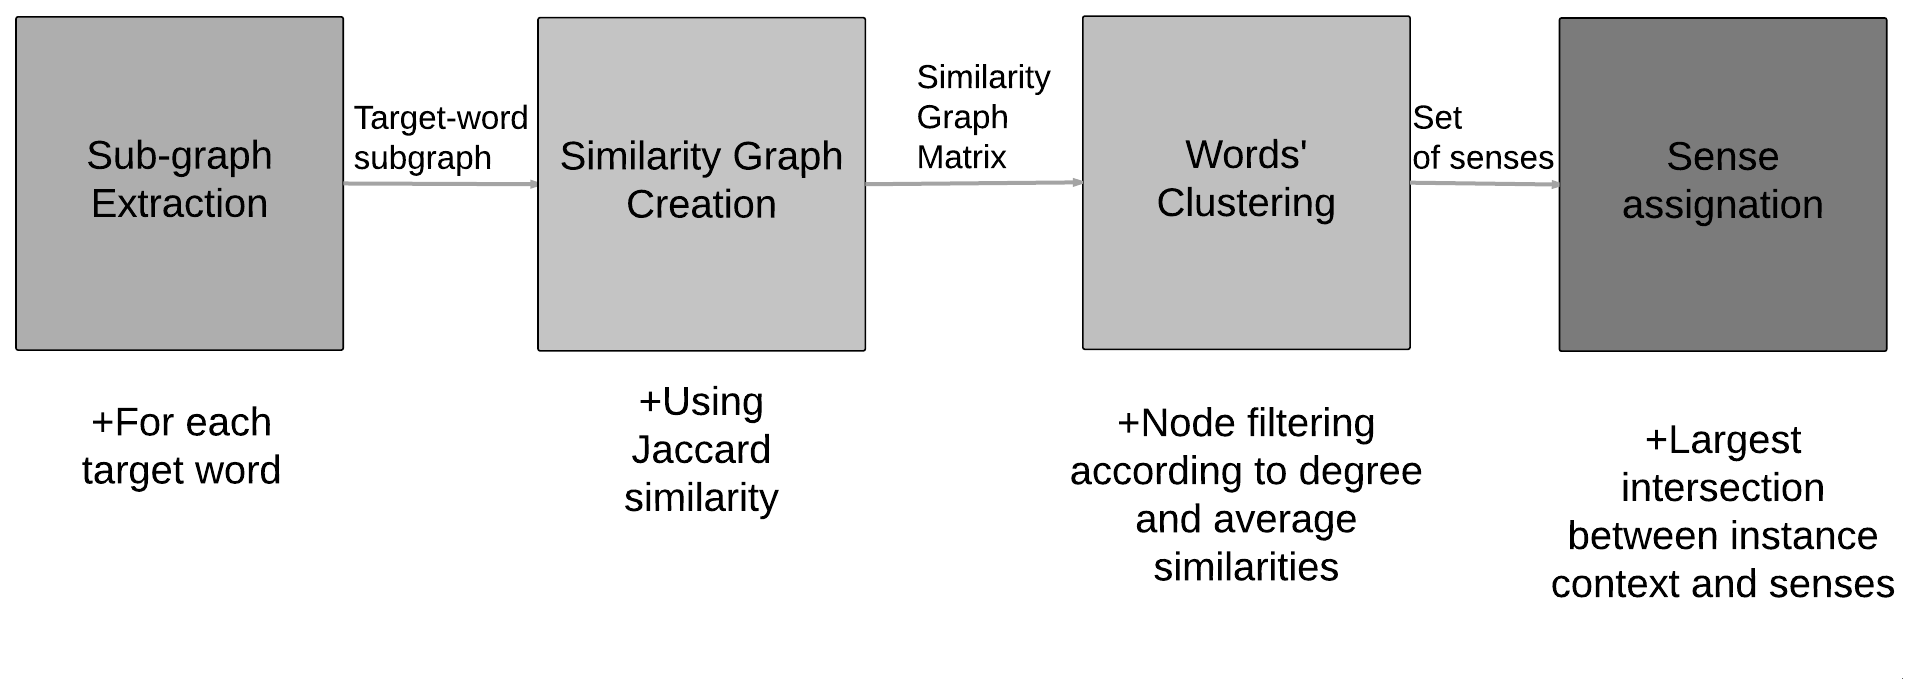
\includegraphics[width=1\linewidth]{images/Chapitre4/wsd_wsi_process.png}
\caption{Block diagram of the WSI/WSD method proposed.}
\label{fig:wsd_wsi_process}
\end{figure}


\paragraph{Creation of the linguistic network}
%In the previous sections we worked with the English Wikipedia as background corpus to build and model our proposed linguistic network. Given the large size of Wikipedia, and to iterate faster our experiments, we decided to change the corpus to one with a more manageable size.

%We use the Open American National Corpus (OANC) \cite{oanc} as background document collection to build a hypergraph network $G_H$ following our proposed model.  The OANC  includes texts from several domains and encompasses 11,406,155 words. We split the documents of the corpus in sentences, then we tokenize and parse them with Stanford's CoreNLP \cite{corenlp}. As described before, the dependency and constituency tree are used to build the hypergraph: words are depicted by nodes, and they may exist inside any of the three different types of hyperedges defined (sentence,  noun phrase or dependency contexts). If any  hyperedge is repeated through the corpus, we increment a counter and keep the number of apparitions instead of adding redundant columns to the hypergraph incidence matrix.

\begin{algorithm}[!htp]
\SetAlgoLined
\KwIn{A set $tw\_set=\{tw_1, tw_2, ..., tw_n\}$ of target words }
\KwIn{A background linguistic network $G_H$}
\KwIn{Filtering thresholds $th_1$, $th_2$}

\KwOut{A set $SoS_{tw}$ of senses for each target word}
\ForEach{target word $tw$ in tw\_set}{
	
	$G_{tw}$ = \texttt{extract\_subgraph}($G_H$, $tw$)\;
	$B_{tw}$ = \texttt{induce\_bipartite\_graph}($G_{tw}$)\;
	$S_{tw}$ = \texttt{sim\_matrix}($B_{tw}$)\;
	$F_{tw}$ = \texttt{induce\_hypergraph}($S_{tw}$, \textit{th1})\;
	$candidate\_hubs$ = \texttt{sort(degree}($F_{tw}$))[:100]\;
	$SoS_{tw}$ = [~]\;
	\ForEach{candidate\_hub in candidate\_hubs}{
%		\uIf{\texttt{degree}(candidate\_hub) $<$ th2}{
%			\textbf{continue}\;
%			}
%		\tcc{get all hyperedges where candidate\_hub appears}
		$candidate\_hyperedges$ = \texttt{get\_hyperedges}($candidate\_hub$, $F_{tw}$)\;
		$candidate\_avg_jaccard$ = 0\;
		\ForEach{ hyperedge in candidate\_hyperedges}{
%		\tcc{get average jaccard of all words (nodes) within hyperedge}
			$candidate\_avg\_jaccard$ += \texttt{get\_avg\_jaccard}($hyperedge$)\;
			}
		\uIf{candidate\_jaccard $>$ th2}{
			$SoS_{tw}$.\texttt{add}(\texttt{get\_words}($candidate\_hyperedges$))\;
%			\tcc{remove hyperedges of candidate hub from tw (filtered) hypergraph.}
			$F_{tw}$ = $F_{tw} \setminus candidate\_hyperedges$\;
		}
	}
	\Return{$SoS_{tw}$}
}

\caption{Pseudo-code of our WSI/WSD network-based approach}
\label{alg:wsd}
\end{algorithm}


In order to find senses from the contexts of a target word, the first step in our procedure is to build a linguistic graph $G_H$ from a background corpus. As described in previous sections, the dependency and constituency trees are used to build the hypergraph: words are depicted by nodes, and they may exist inside any of the three different types of hyperedges defined (sentence,  noun phrase or dependency contexts). If any  hyperedge is repeated through the corpus, we increment a counter and keep the number of apparitions instead of adding redundant columns to the hypergraph incidence matrix.

At each step, that is, for each $tw$ in the test input document, we extract a subgraph $G_{tw}$ from $G_H$ that contains all the words that appear together with $tw$ (line 2), whether by lexical or syntactic co-occurrence. The $tw$ is removed from $G_{tw}$. In this approach we focus specifically on dependency relations and lexical co-occurrence. 

We note that for the syntactic co-occurrence, that is, the dependency relations between words, we apply two strategies: when dealing with a noun target word, we use the co-occurrent relations between said noun and other words having a similar  dependency head token. On the other hand, when dealing with a verb target word, we select the co-occurrent words having said verb as head of the dependency relation.  The reason is that usually verbs are more often than not the head of dependency relations, so the intuition is that words which have the same verb governor are somehow semantically related. %Otherwise, if we took the relations between verbs and other words having a similar dependency head, we would 

\paragraph{Computing the similarity between nodes}
In order to computationally treat $G_{tw}$, we first induce a bipartite graph $B_{tw}=(U,W,E)$ from $G_{tw}$ (line 3). The set of left nodes $U$ represent words and the set of right nodes $W$ depicts the membership to a given hyperedge. Thus, we have as many nodes in $W$  as we had hyperedges in $G_H$.

We compute the Jaccard index between each node $n_{i,j} \in U$ as $Jaccard(i,j)=\frac{|N(i)\cap N(j)|}{|N(i)\cup N(j)|}$ in order to build a $|U|\times|U|$ similarity matrix $S_{tw}$ (line 4). We induce from $S_{tw}$ a new filtered  hypergraph incidence matrix $F_{tw}$ (line 5), which contains word nodes as rows and columns as hyperedges. Each of these hyperedges represent a set of words that are deemed similar between them according to their Jaccard  index value, which must be equal or higher than an assigned threshold $th_1$ .  

\paragraph{Clustering words  together}
Once the incidence matrix $F_{tw}$ is built we can proceed to induce senses for a target word by clustering words (vertices) together. First, we calculate the degree of each node $n_i \in F_{tw}$. The degree of a node is simply the number of hyperedges it is incident in. Nodes are sorted in descending order and evaluated one by one. We consider the top $c$-nodes as sense hub candidates (line 6). We accept or reject a node $n \in F_{tw}$ as a sense carrying word according to one condition. As shown from line 11 to 17 in the pseudo-code, we set a minimum limit to the average of the Jaccard similarities between each pair of neighbors of node $n \in F_{tw}$ within each hyperedge  $n$ belongs to. Formally, for a node $n$, we define the average Jaccard measure as: $$AvgJaccard(n)=\frac{1}{|hedges(n)|}\sum_{h\in hedges(n)}\frac{\sum_{\substack{i\in h\\j\in h;i\neq j}}Jaccard(i,j)}{|h|}$$ 
where $hedeges(n)$ is the set of hyperedges $n$ is incident in and its cardinality is defined as $|hedges(n)|$, and $|h|$ is the number of nodes in the hyperedge $h$. 

The Jaccard similarity measure allows us to easily determine the neighbors of each node in the current bipartite hypergraph representation. As each node is joined to a sentence or dependency node, calculating the Jaccard similarity amounts to determining the level of co-occurrence between each word according to a specific type of hyperedge (represented as a node from the other graph partition) while taking into account the total number of hyperedges the words participate in. We differentiate specifically from the previously described method, UOY, in that in the case of that system, the weighting of the hyperedges is done by computing the average confidence metric of each hyperedge. In this regard, the Jaccard similarity is more flexible with respect to the confidence metric, as the confidence requires in the numerator the number of contexts (paragraphs in UOY's case) shared by all the members of the hyperedge, whereas the Jaccard measure takes pairs of members individually and thus is less strict in the apparition of all the elements of the hyperedge in the contexts. Given the nature of the features used (lexical and syntactical dependencies), we fix our thresholds in a manual but simpler way by defining percentiles and taking the value of the threshold directly, without having to change it according to the characteristics of the data.

If node $n$ satisfies both thresholds $th_1$ and $th_2$, it is deemed as a sense purveyor and all its neighbors (words that appear in the same hyperedges as $n$) are conflated into a single set representing a $tw$ sense. This new sense is added to $SoS_{tw}$ (line 17). The sense set is then removed from $F_{tw}$.

The process is repeated until no more nodes satisfy both boundaries. When the process is complete, we obtain a set of senses $SoS_{tw}$ where each set contains words that ideally represent a unique meaning for each target word. 

\paragraph{Sense assignation}

The assignation of a sense consists in looking at each $tw$ instance represented by a context $ct$ and simply determining which sense $s$ in $SoS_{tw}$ shares the highest amount of words with $ct$. The sense $s$ is thus assigned to that instance. If two senses in $SoS_{tw}$ share the same amount of words with $ct$, one of them is randomly chosen.  This operation is repeated for each instance of each target word. 



	
\paragraph{Experiments and Evaluation}
\subparagraph{Test Datasets}
We trained and evaluated our system on two datasets: Semeval 2007 Task 2 (as in the previous experiments) and Semeval 2010 Task 14 \cite{Semeval2010}. We recall that the Semeval 2007 task consisted in the induction and disambiguation of a single set of 100 words, 65 verbs and 35 nouns, each target word having a set of contexts where the word appear. On the other hand, the Semeval 2010 task consisted also on 100 words, with 50 being verbs and 50 being nouns. This time, a training set from which the senses of a word have to be induced is provided. In our experiment, for the Semeval 2010 dataset, we induce the senses from the training set and disambiguate the target words present within the test set.

We apply a light pretreatment, consisting on token lemmatization and we remove all words that appear less than four times. Concerning the individual graphs of each target word, we work only with nouns and if the extracted graph has fewer than 100 nodes, we do not apply any filtering (we keep all the extracted words). We do this in order to avoid empty solutions.



\subparagraph{Implementation}
The objective of this experiment is to understand the performance of both lexical and syntactic co-occurrence information, used independently, while solving WSI and WSD tasks while using the method described in the previous subsection. To that end we build two independent systems: LEX, which uses exclusively lexical co-occurrence hyperedges, and DEP, which employs only syntactic dependency hyperedges. 
 %
Each type of hyperedge has its own network characteristics as mentioned before. Sentence hyperedges tend to have a much smaller number of words than those of the dependency category. This make sense as sentences usually contain less than 30 words, meanwhile a dependency hyperedge may contain up to hundreds of words (several words may share the same dependency relation). Taking this into consideration we set different threshold values for LEX and for DEP. First, we  consider only the top 100 nodes as candidate sense hubs. Secondly, we do not set the thresholds' values directly but instead we set up a percentile value for the Jaccard similarity ($th_1$) and for the average Jaccard similarity ($th_2$). This is a practical solution to the changing nature of the network model according to the features being employed. We experimentally found the best values for  each threshold used.



%Given that the variation of these thresholds affect the performance of the systems, we decided to experimentally fix threshold $th_1$ at 0.7 for \textit{dep} and at 0.030 for \textit{lex}. The difference of scales is determined by the characteristics stated before, that is, the sparse nature of the sentence hyperedges compared to the density of dependency hyperedges. The second threshold $th_2$ is automatically set for both systems, as explained above.
%
%This leaves only one threshold left, $th_3$. We experiment with two different ranges of values, one for each system. For \textit{dep} we set the range $[0.3, 0.65]$ with a step of 0.05. For \textit{lex} we set $[0.01, 0.08]$ with a step of 0.1. These ranges were chosen experimentally with two constraints in mind: (1) lower threshold values usually gave the same results\footnote{Still, some of the values used produced equal results and thus are not visible in Figure \ref{fig:prec_recall}.} as those already included in our ranges, and (2) higher threshold values forced the system to either give only one sense per word (resulting in the most frequent baseline), or even worse, not accepting any sense, thus having an null solution. 



\paragraph{Results and Discussion}
%Both Semeval 2007 and Semeval 2010 tasks are evaluated by an unsupervised and supervised set of measures. 
\subparagraph{Semeval 2007}

\begin{table}[!htb]
\centering
\caption{Unsupervised F-measure (FM) for the Semeval 2007 test set. Results are obtained with our proposed algorithm.}
\begin{tabular}{@{}lrrrr@{}}
\toprule
\textbf{F-measure (\%)} & \textbf{all} & \textbf{nouns} & \textbf{verbs} & \textbf{\#cl} \\ \midrule
1c1word          & 78.9         & 80.7           & 76.8           & 1.00             \\
UBC-AS           & 78.7         & 80.8           & 76.3           & 1.32          \\
DEP     & 74.9         & 80.2           & 69.0           & 3.27          \\
LEX     & 61.4         & 62.6           & 60.1           & 4.26         \\
UoY(2007)        & 56.1         & 65.8           & 45.1           & 9.28          \\
Random           & 37.9         & 38.1           & 37.7           & 19.7             \\
1c1instance & 	9.5         & 6.6           & 12.7           & 48.51             \\ \bottomrule
\end{tabular}

\label{tab:sem2007_unsup_FS}
\end{table}

In Table \ref{tab:sem2007_unsup_FS} we present the unsupervised evaluation results for our models as well as for some other systems. We include the F-measure as performance metric. 

In this table, as in the rest of the tables presented in this section, the columns show the results for all the words, for the nouns exclusively as well as for the verbs. The final column indicates the number of induced clusters per system. It is important to consider this value as the unsupervised metrics are biased towards systems with less number of induced clusters and thus to the 1c1word baseline.

We can appreciate that both our methods surpass the baselines and the system described before \textit{UoY(2007)}. The best system of the competition, \textit{UBC-AS} used also co-occurrence graphs and applied a random-walk based clustering algorithm over the vertices' similarity matrix. Still, our system induced a larger amount of senses, while retaining a competitive F-measure value. We also note that in this evaluation DEP, the system using only co-occurrent dependency relations outperformed the lexical co-occurrence only system LEX.

\begin{table}[!htb]
\centering
\caption{Supervised Recall (SR) on the Semeval 2007 test set. Results are obtained with our proposed algorithm.}
\begin{tabular}{@{}lrrrr@{}}
\toprule
\textbf{Recall (\%)} & \textbf{all} & \textbf{nouns} & \textbf{verbs} & \textbf{\#cl} \\ \midrule
I2R & 81.6 & 86.8 & 75.7 & 3.08 \\
LEX & 79.4 & 82.5 & 75.9 & 4.26 \\
DEP & 79.1 & 81.5 & 76.4 & 3.27\\
MFS & 78.7 & 80.9 & 76.2 & 1 \\
UoY(2007) & 77.7 & 81.6 & 73.3 & 9.28 \\ \bottomrule
\end{tabular}

\label{tab:sem2007_sup_recall}
\end{table}


Moving onto the supervised results for Semeval 2007, in Table \ref{tab:sem2007_sup_recall} we show the results obtained concerning the Recall performance metric.  In this table we include the competing system \textit{I2R} \cite{Niu2007}, based on an Information Bottleneck based clustering algorithm, which obtains the best results according to all the words and nouns. Both our systems DEP and LEX beat the baseline of assigning the most frequent sense to an instance MFS). More interestingly, DEP was able to beat the MFS verb baseline, something that was not achieved during the competition. As was the case before, our systems beat UoY(2007).




As a way of determining where does both systems complement each other, in Figure \ref{fig:nouns_fs} and Figures  \ref{fig:verbs_fs2} and \ref{fig:verbs_fs3} we show the unsupervised F-measure value for nouns and verbs respectively (we split the verbs in two figures for visibility). We can see that, as the previous result tables indicated, DEP did better overall. Nonetheless, and what is most interesting in these figures, is that there are certain words (both nouns and verbs) that obtain better scores using LEX instead of DEP and vice versa. For example, the nouns \textit{area}, \textit{future}, and \textit{state} are better treated by LEX, according to this measure, even if by a small margin. On the other hand, with respect to the verbs, the differences between performance are more important. Again, the LEX system does better while finding senses and assigning them to the verbs \textit{avoid}, \textit{fix}, and \textit{work}. %This information will be useful during the design of hybridization techniques between feature of our hypergraph structure.

 




 \begin{figure}[!htb]
\centering
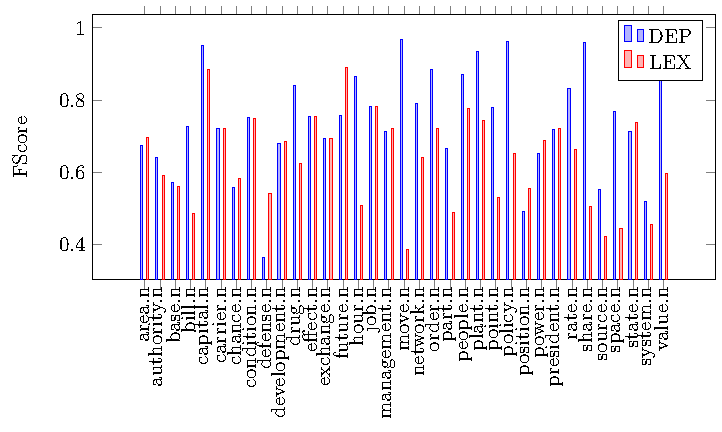
\includegraphics[width=1\linewidth]{images/Chapitre5/tex_img_files/nouns_fs.pdf}
\caption{Unsupervised F-measure results for the nouns of the Semeval 2007 test set.}
\label{fig:nouns_fs}
\end{figure}

 \begin{figure}[!htb]
\centering
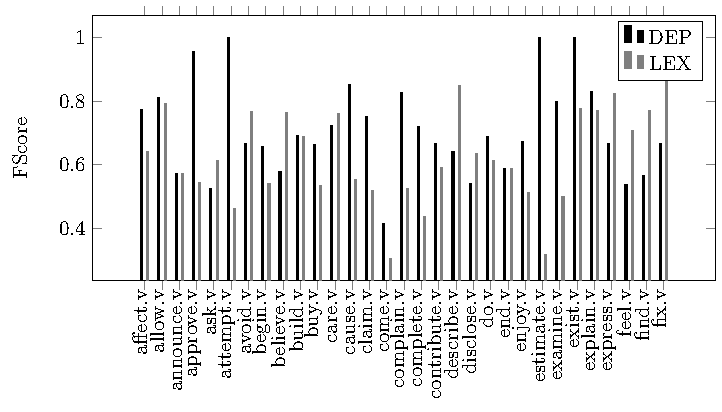
\includegraphics[width=1\linewidth]{images/Chapitre5/tex_img_files/verbs_fs_2.pdf}
\caption{Unsupervised F-measure results for the first half of verbs of the Semeval 2007 test set.}
\label{fig:verbs_fs2}
\end{figure}

 \begin{figure}[!htb]
\centering
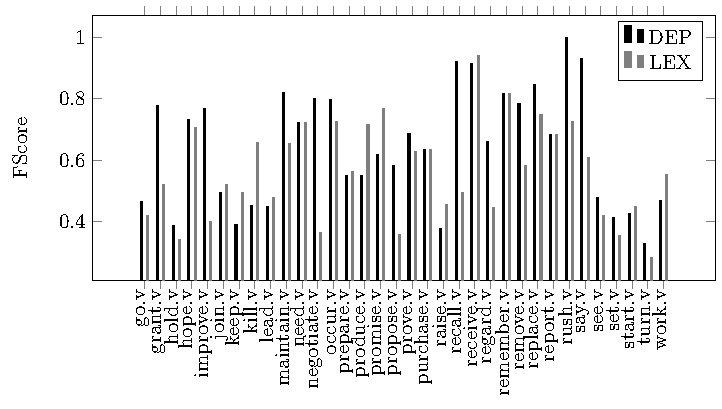
\includegraphics[width=1\linewidth]{images/Chapitre5/tex_img_files/verbs_fs_3.pdf}
\caption{Unsupervised F-measure results for the second half of verbs of the Semeval 2007 test set.}
\label{fig:verbs_fs3}
\end{figure}

%todo add phrase that says that syntactic is not as good as seen in the paper where they compare a lot of distributional models... 	


%todo split verbs?
\subparagraph{Semeval 2010}
In Semeval 2010, two unsupervised evaluation metrics are introduced: \textit{V-Measure} and \textit{paired F-measure}. Briefly, the V-Measure assesses the quality of a clustering solution by measuring the degree to which each cluster consists of instances principally belonging to a single gold standard class, or homogeneity; and to completeness, the level with which each gold standard class consists of instances primarily assigned to a single cluster.

The paired F-measure evaluation transforms the clustering problem into a classification one. Two instance pairs sets are generated, the first one coming from the system induced clusters, by including pairs of the instances found in each cluster. The second set of instance pairs is built from the gold standard classes. It contains pairs of the instances found in each class. We can then define \textit{Precision} and \textit{Recall}. Precision is computed as the ratio of the number of common instance pairs between the two sets divided by the total number of pairs in the clustering solution. Recall is the count of common instance pairs between the two sets divided by the total number of pairs in the gold standard. The paired F-measure is the harmonic mean of both quantities.

Concerning the supervised evaluation, it follows explicitly that of Semeval 2007, using recall as the main performance measure as in  \cite{Semeval2010,VandeCruys2011,pedersen2010duluth}.

\begin{table}[]
\centering
\caption{Unsupervised V-Measure (VM) on the Semeval 2010 test set. Results are obtained with our proposed algorithm.}
\begin{tabular}{@{}lrrrr@{}}
\toprule
\textbf{V-measure (\%)} & \textbf{all} & \textbf{nouns} & \textbf{verbs} & \textbf{\#cl} \\ \midrule
{Hermit} & 16.2 & 16.7 & 15.6 & 10.78 \\
NMF$_{lib}$&11.8&13.5&9.4&4.80\\
LEX & 11.6 & 8.8 & 11.9 & 10.5 \\
Random & 4.4 & 4.2 & 4.6 & 4.00 \\
DEP & 3.5 & 3.9 & 2.8 & 2.75 \\
MFS & 0.0 & 0.0 & 0.0 & 1.00 \\ \bottomrule
\end{tabular}

\label{tab:sem2010_VM}
\end{table}

In Table \ref{tab:sem2010_VM} we present our systems compared to the baseline and other methods using during Semeval 2010. V-Measure is a metric well-known for favoring systems producing a higher number of clusters \cite{VandeCruys2011,pedersen2010duluth}. Thus, it is considered not a very reliable metric. We have included it to have a global insight about the performance of our method. We remark that only LEX performed better than both baselines, random assignation of senses (Random) and using the most frequent sense (MFS). Also, we note that we included only the best performing systems, in this case \textit{NMF$_{lib}$} and  \textit{Hermit}. The former  did not participate on the competition but was developed later. We include it henceforth to illustrate how systems variate from one position to another depending the metric used to assess the performance. The latter was the best method on this metric from the task challenge. It is important to notice that other systems exist between Hermit and LEX. They were not included for the sake of clarity.

\begin{table}[]
\centering
\caption{Unsupervised Paired F-measure (FM) for the Semeval 2010 test set. Results are obtained with our proposed algorithm.}
\begin{tabular}{@{}lrrrr@{}}
\toprule
\textbf{F-measure (\%)} & \textbf{all} & \textbf{nouns} & \textbf{verbs} & \textbf{\#cl} \\ \midrule
MFS & 63.5 & 57.0 & 72.4 & 1.00 \\
Duluth-WSI-SVD-Gap & 63.3 & 57.0 & 72.4 & 1.02 \\
DEP & 53.6 & 50.1 & 58.7 & 2.75 \\
NMF$_{lib}$&45.3&42.2&49.8&5.42\\
LEX & 38.4 & 46.7 & 28.5 & 10.5 \\
Random & 31.9 & 30.4 & 34.1 & 4.00 \\ \bottomrule
\end{tabular}

\label{tab:sem2010_FS}
\end{table}

The second unsupervised measure, Paired F-measure, can be seen in Table \ref{tab:sem2010_FS}. In this case both systems presented performed better than the random baseline. Any system presented was able to beat the MFS baseline. We note that DEP does much better compared to LEX concerning verbs, namely 58\% vs. 28\% F-measure. Still, the results are low considering the best results of the competition, 63\% from Duluth, although again, it generates a number of senses very similar to the MFS baseline. Both our systems induce a considerable amount of clusters while keeping a descent F-measure.



\begin{table}[tb]
\centering
\caption{Supervised recall (SR) for Semeval 2010 test set (80\% mapping, 20\% evaluation). Results are obtained with our proposed algorithm.}
\begin{tabular}{@{}lrrr@{}}
\toprule
\textbf{Recall (\%)} & \textbf{all} & \textbf{nouns} & \textbf{verbs} \\ \midrule
NMF$_{lib}$&62.6&57.3&70.2\\
UoY(2010) & 62.4 & 59.4 & 66.8 \\

LEX & 59.8 & 55.8 & 67.4 \\
DEP & 59.3 & 53.9 & 67.2 \\
MFS & 58.7 & 53.2 & 66.6 \\
Random & 57.3 & 51.5 & 65.7 \\ \bottomrule

\end{tabular}


\label{tab:sem2010_SR}
\end{table}


Finally, we in Table \ref{tab:sem2010_SR} we show the supervised Recall results of Semeval 2010. The best performing algorithm shown is NMF$_{lib}$. During the competition, UoY(2010) was the best method. It is a graph-based algorithm which shares the name with the UoY  system presented in Semeval 2007, but it is a different  approach. 

Concerning our systems, in this evaluation they seem to perform the best, or in a comparable level, to the top methods.  We find that in general our systems seem to perform better on the Semeval 2007 dataset. Discovering the reason could shed light into improving the performance on the Semeval 2010 test set. Given the results, it seems like a combination of features (syntactic plus lexical) in  a single algorithm could yield better results. 

As a side note, it is argued that supervised Recall is not a very robust metric as the supervised method within tends to converge towards the most frequent sense. In this regard, several researchers \cite{VandeCruys2011,pedersen2010duluth} have voiced their concerns about the quality of the current WSI/WSD evaluation metrics as well as the need of new, more robust techniques to properly evaluate these systems.



%\paragraph{Conclusion}

\section{Conclusion}
\label{chap6:conclusion}
In this chapter we addressed two NLP tasks from two different points of view: on the one hand, we computed several representation spaces using fusion operations in order to enrich and densify otherwise sparse and independent features. The matrices generated were used to train both supervised and unsupervised models to solve named entity recognition and word sense induction and disambiguation.

On the other hand, we proposed a model that leverages the inner structure of the hypergraph network to group words that belong to a shared sense. This approach was used to solve word sense induction.

More specifically, concerning the first part, we presented  a comparative study of multimedia fusion techniques applied to named entity recognition.  We also tested hybrid fusion recombinations in order to complement the information contained in the single representation matrices. In order to accomplish this goal, we built upon basic fusion techniques such as early and late fusion, as well as cross media fusion to transfer quality information from one set of features to another. 

%We found that by taking a strong feature, in our case lexical context, $\mlex$, and enriching it with the output of rather complex fusion combinations, we can improve the performance of the tasks addressed. The enrichment has to give more relevance to the strong feature matrix, by selecting the right parameters. 

We analyzed the results to understand how the enrichment of features improved the performance. We found that at each fusion step, a different type of NER tag is benefited. We studied what features where driving the decision towards the correct class and found that while the enriched features are not the most prominent  in the decision function, they play an important role by tipping said decision towards the correct label and away from the wrong one. 

Concerning fusion enrichment and WSI/WSD, we found that the fusion operations also improve the results of the task, although not as clearly as in NER. The metrics used to measure the performance on this ask does not allow a clear understanding on the behavior of the model employed. While we want to avoid converging to the trivial one sense per word solution, we know that words do not have numerous senses. In that sense, the results obtained stay reasonably away from the trivial solution while not producing many senses as other approaches.

While there is an improvement using fusion techniques, we do note that they  enlarge the feature space, especially early fusion, which is used frequently. This may imply the need of larger quantities of memory and longer execution time. In that sense, as future work, more intelligent ways of finding the most appropriate fusion must be researched. This is indeed one of our future work paths: determining an optimal fusion path from single features to a high degree fusion recombination. Coupled with this, the automatic determination of the parameters is still ongoing research in the multimedia fusion community. Consequently, we believe that efficiently determining both parameters and fusion combinations is the general domain of our future work. Another route we would like to explore is testing these techniques on other tasks and with datasets from different domains, in order to assert its effectiveness.


% WSD network
Concerning our proposed network-based method, we show how using the inner links within the hypergraph structure we can group words that represent senses and then assign them to target words. Our method distinguishes from similar works in two main aspects: the definition of similarity used, the reduced number of parameters that are needed, the use of diverse types of contexts to solve the task. 	We show that our method beats said similar approaches. Also, we discovered the behavior of syntactic contexts in comparison to lexical contexts at word-level. Indeed, lexical contexts seem to perform better. This is in line with other works on distributional representations \cite{kiela2014systematic}.



%\minitoc

%\subsubsection{Introduction}

%

\chapter{Wikipedia Syntactic Dump}
In order to have a working dataset, we first built a software that process and parse any input corpus. We describe its properties, its inputs, the information extracted, as well as the output generated by the software.



\section{Introduction and Related Work}
%Today, the broad reach of Wikipedia in Text Mining (TM) and Natural Language Processing (NLP) research  is indisputable. Several recent approaches and tools have  been conducted based on the explicit and implicit knowledge contained in it. Certainly, Wikipedia provides a common ground for researchers and developers to test and compare their results.

The online encyclopedia Wikipedia has been used as a source of valuable data as well as a common background corpus to perform experiments and compare results for diverse NLP/TM related tasks. For example, concerning the first case, in the area of Information Extraction, Wikipedia's infoboxes structured information is used in \cite{Wu2010} as a valuable resource to complement and improve their open IE system. Along the same line, \cite{charton2010}  extracted metadata from Wikipedia while leveraging its internal structure in order to produce a semantically annotated corpus. Moving on to the Information Retrieval field, features extracted from Wikipedia can also help to better predict the performance of a query  \cite{katz2014} in a given  corpus.  In the second case, as a background collection for experiments, a document-aligned version of English and Italian Wikipedia has been used to determine the quality between word's translations \cite{vulic2011}.  

Wikipedia, being such a popular resource  already has various off-the-shelf parsed snapshots (or dumps). These parsed dumps allow researchers to focus more into their approaches than into the extraction and transformation of Wikipedia's data.  We briefly describe certain relevant parses found in the literature.   
%



%The already mentioned parsed dump from \cite{ATSERIAS08}
A relevant Wikipedia parsed dump example comes from \cite{ATSERIAS08}. Their work provides a balanced amount of syntactic and semantic information. In short, the dump includes each word's Part-of-Speech (PoS) tag, their dependency relations as well as the output of three different named entity recognition parsers. Additionally, they provide a graph structure that leverages Wikipedia's internal composition alongside its corresponding metadata. Nonetheless, the resource is no longer available on the original URL although it may be obtained through Yahoo's Webscope\footnote{\url{https://webscope.sandbox.yahoo.com/}} datasets library.  In \cite{FLICKINGER10}, they perform a deep parse analysis is performed to provide detailed syntactic and semantic information. The authors leverage a previously manually annotated portion of the English Wikipedia. They extract a grammar from this portion and also train a statistical model  to automatically parse the rest of Wikipedia. Even though the parse offered is deep and rich in details, the annotation labels, as well as the corpus output format, may not be convenient and easy to use because of its complexity and particular nature. \cite{SchenkelSK07}  released a purely semantic XML parse that links WordNet concepts to Wikipedia pages. They focus greatly on cleaning and pre-treating Wikipedia. In this paper we do not focus as much into the cleaning of Wikipedia as already available tools can solve the task quite well for non-specific needs. 
Finally, there are certain Wikipedia dumps that offer the raw cleaned text without any extra subsequent parsing or analysis. Such is the case of the corpus made available by \cite{westbury2010}. This corpus makes  use of the \textit{WikiExtractor} script  \cite{Attardi2015} to clean the Wikipedia dump.
  
  
Although the existing parses and dumps already satisfy numerous specific research needs, they have certain limitations that drove us to build our own resource: the Syntactically Annotated English Wikipedia  Dump (SAEWD). Specifically, we address the following shortcomings: the lack of constituents-based tree information, the complex output formats, the limited online access and the absence of the tools used (i.e., the source code) to create the annotated corpus. In SAEWD we include the complete parse tree information for each word provided by well-known parsing tools. We store the extracted information in a simple and already existing output format. Additionally, we give open access to the parsed dump and we share our source code with the community. The code allows anyone (with programming skills) to  apply our processing pipeline and build their own particular Wikipedia parse or even to parse other text collections. Finally, we present and provide a hypergraph linguistic network for fast NLP/TM experimentation. Indeed, SAEWD aims to be used as a stepping stone for a standard Wikipedia parsed version for the largest possible set of tasks in future research. 

SAEWD uses widely known English language parsing tools, namely those included in the Stanford CoreNLP suite.  Aside from being accessible and regularly maintained, it provides a common set of labels (Universal Dependencies\footnote{\url{http://universaldependencies.github.io/docs/}}) used by numerous NLP and TM experiments. Regarding SAEWD output's format, we believe that the file format we use, which follows  that of \cite{ATSERIAS08}, allows for fast reading and simple interpretation. Among other syntactical information, we provide the constituents parse branch for each word (explained in detail in Section \ref{text:description}). 
Constituent's paths, and hence chunk's production rules, have been proved useful as a complement feature to classic text representations \cite{sagae2009,Bergsma2012,Massung2013}. 
%This information is commonly missed by most Wikipedia parses. It may be due to the fact that it may not be easy or clear to use the constituents nodes information; or may be because storing a tree branch is not as straightforward as stocking a single relationship type label, as is the case of a dependency parse.

As a second contribution, we propose a hypergraph linguistic representation. Over the past few years, research on the NLP domain has been focusing on novel techniques that take advantage of the characteristics of language networks to achieve new and interesting results \cite{Mihalcea11}. That is why, in addition to SAEWD, we also propose, as a proof of concept, a hypergraph representation that stores certain information found in a SAEWD in a practical way that allows for fast and effortless data extraction. This hypergraph can be indeed considered as a Linguistic Network \cite{Choudhury09}.  It aims to facilitate the implementation of graph-based approaches by allowing researchers to jump directly into the algorithm development stage. We use a sub-sample of the Wikipedia corpus consisting of articles related to Natural Language Processing and Text Mining. 
% Our parsed dump,  the source code used to generate it, the network and its metadata will be online and available for LREC 2016.

In the following sections we describe the steps we undertook to transform a Wikipedia dump into SAEWD (Section 2), we give a detailed account of the contents of SAEWD and the format in which we stored the parsed information (Section 3), then we explain the characteristics of our proposed network structure (Section 4). Lastly, we present our final comments on the nature of the work done as well as possible future work perspectives.




\begin{figure}[t]

	\centering
	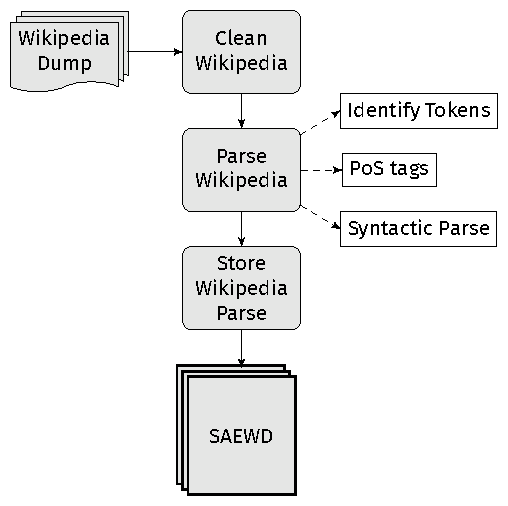
\includegraphics[scale=.8]{images/Chapitre7/flow_chart.pdf}
	\caption{The tree steps we took to build SAEWD.}
	\label{fig:flow}

\end{figure}

\section{Construction of SAEWD}
The three main steps we followed to build SAEWD are presented in Figure \ref{fig:flow}. Briefly, we have one input, which is the Wikipedia dump and one output which is the parsed snapshot. In the following we provide a detailed description of each of the process. 

 
We begin the construction of the parsed corpus with the Wikipedia dump XML file obtained from the Wikipedia database\footnote{\url{https://dumps.wikimedia.org/enwiki}} from early November 2014. This dump  contains around 4.7 million article pages\footnote{We kept all articles available in the Wikipedia dump.}. As shown in Figure \ref{fig:flow}, we apply the following processing steps in order to yield the final parsed version.
 
\subsection{Cleaning Wikipedia} First, we discard Wikipedia's  tables, references and lists, markup annotations and HTML tags with the \textit{WikiExtractor} \cite{Attardi2015}  script. 
We used this tool to clean and split the content of the original XML file into 429 folders each one containing 100 files of approximately 300 kB. These files contain a certain number of complete Wikipedia articles which is automatically determined by WikiExtractor  according to the maximum possible size assigned for each file, 300 kB in our case, thus the number of articles in each file may vary. We decided to use numerous files as well as a small size to easily read their content into memory while parsing. Having multiple small files also makes it easier to handle the multi-threading aspect of our parsing tool.
We kept WikiExtractor's original folder nomenclature which assigns to each one of them a sequence of letters sorted lexicographically\footnote{We have folders named \textit{AA}, \textit{AB}, \textit{AC} and so on.}. The files containing the cleaned text is simply named \textit{wiki\_XX} where  \textit{XX} goes from 00 to 99, as we have 100 files per folder. 
It is important to note that the Wikipedia articles' titles themselves are not sorted in any specific way, as it was not in the interest of our research to have them ordered. 
Inside each cleaned file, besides the article's text, WikiExtractor keeps the original article's URL as well as its unique Wikipedia ID within an XML-like label that also doubles as  article separator. 

\subsection{Parsing Wikipedia} Next, once the Wikipedia dump had been cleaned, we use the Stanford CoreNLP\footnote{\url{http://nlp.stanford.edu/software/corenlp.shtml}} \cite{manning2014} analysis tools to parse all the file texts produced during the previous step. As a part of our processing pipeline, we first perform  sentence segmentation, word tokenization and lemmatization. Below, we briefly describe each of the extracted attributes. We also exemplify them in detail in Section \ref{text:description}.
\begin{itemize}
\item PoS tagging: We obtain the grammatical category of each word, i.e., the part-of-speech tag, using the CoreNLP default tagger, the \textit{left3words} PoS tagging model.
\item Dependency parse: this attribute consists on an extracted tree that describes the types of grammatical relations between words, i.e., the dependency-based parse tree. 
The analysis was performed with the Stanford's \textit{Shift-Reduce}  parser.
% This parser is known to perform better than other Stanford parsers.                                  
 %(notably  faster and  with stronger \textit{F1} measure than the previous PCFG parser, although not as accurate as the Recurrent Neural Network system trained with semantic word vectors).
As information representation, we use the basic dependencies scheme, as we wanted to include each one of the possible dependency relations without any collapsing between them.    
                                                                                                                                                                                    
                                                                                                                                                                                    
\item Constituents parse:                                                                                                                                                           
the output of this analysis is a rooted tree that represents the syntactic structure of a phrase.                                                                                  
This tree is commonly known as the constituency-based parse tree.                                                                                                                  
For each word, we store its complete path in the constituency tree.
 Specifically, we keep all the nodes of a word's own branch from the root to the word itself.
 We employ the Stanford Shift-Reduce parser.
 This path is transformed into a single line and included in SAEWD. 
 

\end{itemize} 	
%\section{Parsed files organization}
 Finally, once the parsing process is complete, the parsed files are stored into individual files and thus there are as much parsed files as input Wikipedia cleaned files. The parsed files keep their original name plus the \texttt{parsed} extension, e.g., \texttt{wiki\_00.parsed}. The structure within the files is described in Section \ref{section3.2}. After parsing, we found the statistics shown in Table \ref{tab:corpus_stats}.
 
\begin{table}[t]
\centering
\caption{English Wikipedia dump statistics.}
\label{tab:corpus_stats}
\begin{tabular}{lr}
{\bf Number of tokens}      & 1,889,769,908 \\
{\bf Unique tokens (types)} & 8,761,691 \\
{\bf Number of sentences}   &  84,760,512\\
{\bf Average number of tokens per sentence} & 22.30
\end{tabular}
\end{table}

\section{SAEWD Description}\label{text:description}
In this section we describe in detail the characteristics of SAEWD.




\begin{table*}[ht]
\centering
\caption{Extract of a Wikipedia parsed file. The phrase shown is the parse result of the previous example sentence in Figure~\ref{fig:tree} }
\label{tab:parse}
\noindent\makebox[\textwidth]{%
\begin{tabular}{llllll}
 \multicolumn{6}{l}{\textit{FILENAME wiki\_00.parsed}}                                           \\ \hline
  \textbf{token}   & \textbf{lemma}   & \textbf{POS} & \textbf{constituency}                      & \textbf{head} & \textbf{dependency} \\ \hline
 \multicolumn{6}{l}{\textit{\%\%\#PAGE Anarchism}}                                         \\ \hline
  {$\vdots$}      &      {$\vdots$}   &  {$\vdots$}   &     {$\vdots$}                              &    {$\vdots$}  &     {$\vdots$}       \\  \hline
 \multicolumn{6}{l}{\textit{\%\%\#SEN 25  9}}                                             \\ \hline
						 A       & a       & DT  & NP\_22,S\_97                      & 3    & det        \\ %\cline{2-7} 
                         great   & great   & JJ  & NP\_22,S\_97                      & 3    & amod       \\ %\cline{2-7} 
                         brigand & brigand & NN  & NP\_22,S\_97                      & 4    & nsubj      \\ %\cline{2-7} 
                         becomes & become  & VBZ & VP\_44,S\_97                      & 0    & root       \\ %\cline{2-7} 
                         a       & a       & DT  & NP\_18,NP\_20,VP\_44,S\_97        & 6    & det        \\ %\cline{2-7} 
                         ruler   & ruler   & NN  & NP\_18,NP\_20,VP\_44,S\_97        & 4    & xcomp      \\ %\cline{2-7} 
                         of      & of      & IN  & PP\_57,NP\_20,VP\_44,S\_97        & 9    & case       \\ %\cline{2-7} 
                         a       & a       & DT  & NP\_18,PP\_57,NP\_20,VP\_44,S\_97 & 9    & det        \\ %\cline{2-7} 
                         Nation  & nation  & NN  & NP\_18,PP\_57,NP\_20,VP\_44,S\_97 & 6    & nmod       \\ %	\cline{2-7} 
\hline 
      
\end{tabular}}
\end{table*}

% Please add the following required packages to your document preamble:
% \usepackage{multirow}
% \usepackage{graphicx}
\begin{table*}[ht]
\centering
\resizebox{\textwidth}{!}{%
\begin{tabular}{cl|cccc|cccc|c}
\multirow{2}{*}{\textbf{PoS Tag}} & \multirow{2}{*}{\textbf{Token}} & \multicolumn{4}{c}{\textbf{NP}} & \multicolumn{4}{c}{\textbf{DEP}} & \multicolumn{1}{l}{\textbf{SEN}} \\ 
 &  & \multicolumn{1}{c}{$ \text{NP\_22}_1 $} & \multicolumn{1}{c}{$ \text{NP\_20}_1 $} & $ \text{NP\_18}_1  $& \multicolumn{1}{c}{$ \text{NP\_18}_2 $} & nsubj\_become & xcomp\_become & nmod\_ruler & \multicolumn{1}{c}{amod\_brigand} & \multicolumn{1}{l}{$ \text{~~S}_1 $} \\ \cline{1-11} 
\multirow{3}{*}{\textbf{NN}} & \multicolumn{1}{l|}{brigand} & 1 &  &  &  & 1 &  &  & & 1 \\
 & \multicolumn{1}{l|}{ruler} &  & 1 & 1 &  &  & 1 &  &  & 1 \\
 & \multicolumn{1}{l|}{nation} &  & 1 &  & 1&  &  & 1 &  & 1 \\ \hline
\textbf{VB} & \multicolumn{1}{l|}{becomes} &  &  &  &  &  &  &  & & 1 \\ \hline
\textbf{JJ} & \multicolumn{1}{l|}{great} & 1 &  &  &  &  &  &  & 1 & 1 \\ \hline
\end{tabular}
}
\caption{Brief example of the linguistic network incidence matrix of the previous used phrase. On the left side, as on the top, we can see the metadata we store for each word (rows) and each column (hyperedges). We omit the rest of the words from the example phrase for brevity.  }
\label{ref:incidence}
\end{table*}

\subsection{Constituency parse storage in detail}
%The  result from the constituency parse is not as straightforward to store as the other kinds of parses, i.e., the output is  a deeper tree structure than that of a dependency parse. Thus, we believe that the storage of this information in SAEWD requires a more in detail explanation. 
%In this subsection, we will describe how we stock the information concerning  the phrases' constituents. 

We will use an example to better explain the storage of the constituency-based parse tree. In Figure \ref{fig:tree} we can see the constituency parse of the phrase  \textit{A great brigand becomes a ruler of a Nation}. On the bottom of the figure, we observe the constituent's path (or branch), of the words \textit{brigand} and \textit{Nation}. As in any tree structure, each leaf node has a defined path from the root node to itself. In this example, the leaf containing the noun \textit{brigand} 
%(PoS tag \textit{NN})
 follows the bottom-up path \textit{NP22}$\rightarrow$\textit{S97}. \textit{Brigand's} parent node is a Noun Phrase (NP) node which in turn comes from the root of the tree, the Sentence node \textit{S}. We assign to each phrase chunk an identifier (22 and 97 in this case) in order to distinguish them according to their building elements as specified by the grammar rule used.
  In other words, a phrase chunk, e.g., a NP, a Verbal Phrase (VP), a Prepositional Phrase (PP), or other chunk defined by the grammar in CoreNLP, may be built from different types of PoS tags. Thus, again from Figure \ref{fig:tree}, we see that the sentence \textit{S97} is  built both from a NP and a VP chunk. 
 In a similar way, the noun phrase \textit{NP18} is produced by a determinant (DT) and a noun (NN), while  \textit{NP22} is generated by a determinant, an adjective (JJ) and a noun.
  The identification digits are obtained from the hash code that represents each chunk object inside our Java application. For each phrase-chunk tree node, we keep the last two significative figures produced by the \texttt{hashCode}\footnote{Java \texttt{hashCode} function description: \url{https://en.wikipedia.org/wiki/Java\_hashCode\%28\%29}} Java method.

\forestset{
    sn edges/.style={for tree={parent anchor=south, child anchor=north}},
    blue text/.style={for tree={text=blue!70}}}

\begin{figure}[]
\resizebox{\linewidth}{!}{%
\begin{forest} 
[S97
	[NP22 [DT [A, blue text]] [JJ [great, blue text]] [NN [brigand, blue text]]]
    [VP44 [VBZ [becomes, blue text]]
      [NP20
        [NP18 [DT [a, blue text]] [NN [ruler, blue text]]]
        [PP57 [IN [of, blue text]]
          [NP18 [DT [a, blue text]] [NN [Nation, blue text]]]]]]]
	\node [draw,fill = blue!20,text width=21em] at (1.5,-6.8) (sparse) {\textbf{brigand} (NN): NP22$\rightarrow$S97 \\ \textbf{Nation} (NN): NP18$\rightarrow$PP57$\rightarrow$NP20$\rightarrow$VP44$\rightarrow$S97};
\end{forest}
}

\caption{Constituency tree for the phrase \textit{{A great brigand becomes a ruler of a Nation}.}
% On the bottom, we can see the bottom-up path stored for the words \textit{brigand} and \textit{Nation}.
}
\label{fig:tree}
\end{figure}

 


As another example, the noun \textit{Nation} has the following bottom-up constituency path: \textit{NP18}$\rightarrow$\textit{PP57}$\rightarrow$\textit{NP20}$\rightarrow $\textit{VP44}. Indeed, the string \texttt{NP\_18,PP\_57,NP\_20,VP\_44,S\_97}, originating from the previously described path,  is the information we keep about the constituency parse for each token in the Wikipedia dump.



\subsection{Annotation scheme}\label{section3.2}
To store the parsed text we use a scheme  inspired by that used in \cite{ATSERIAS08}. The format can be considered as a regular tsv file (i.e., the entries are separated by tab spaces) with additional metadata tags. An extract from a parsed file can be observed in Table \ref{tab:parse}. 

The file includes two headers: the first one simply indicates the name of the current parse file; the second one contains the names that describe each column. The tags and columns our parsed dump contains are the following:
\begin{itemize}
\item Metadata tags:
\begin{enumerate}
\item {FILENAME}: indicates the original file used to extract the current parse, 
\item {\%\%\#PAGE}: denotes a new Wikipedia article, as well as its title, 
\item {\%\%\#SEN}: marks the beginning of a new sentence. It is followed by two integers: (1) the number of the current sentence, and (2), the number of tokens in the sentence.

\end{enumerate}

\item Parse columns for each token:
\begin{enumerate}
\item Token: the token itself,
\item Lemma: the token the canonical form,
\item POS: its part of speech tag,
\item Constituency: the bottom-up constituency path described before,
\item Head: the head index of the dependency relation the current token belongs to,
\item Constituency: the name of the grammatical relationship this token participates in as a dependent.
\end{enumerate}
\end{itemize}

Using the example phrase introduced before (Table \ref{tab:parse}), the token \textit{becomes} has \textit{become} as lemma, it is a verb, thus it has \textit{VBZ} as PoS tag, its constituency path is \textit{VP\_44,S\_97}, so it belongs to the verb phrase {VP44} which in turn comes from sentence {S97}. Finally, \textit{becomes}, being the main verb, is in this case the grammatical root of the sentence and its head is by convention determined as  zero. 

Concerning the computation time, SAEWD takes around 40 hours to be produced using a general purpose laptop (Intel i7 4700MQ with 4 cores, 8 GB and Linux Mint 17 as operative system). Most of the time is taken by the parsing step. 

We verified the consistency of the corpus built by analyzing a sample of 20 Wikipedia articles. The output of CoreNLP and the information contained in the corpus match.



\chapter{Conclusions and Future Work}
\label{chap:conclusions}
%\minitoc
\section{Conclusion}
Linguistic Networks are useful methods to understand the nature of our language. In the literature, they are generally used to comprehend either the dynamics of words and other textual units within language, and to solve practical NLP tasks. Nonetheless, no mater the objective, they are usually based on the distributional hypothesis, that is, words will be found in similar contexts if they tend to be semantically related.

Distributional models are based on several parameters, such as the size of the context to be used, their linguistic type (either syntactic, lexical, etc.), the weight that affects each context-word co-occurrence, as well as determining how the semantic relatedness is computed. Indeed, most of the linguistic networks in the literature deal with a single type of contexts, either lexical or syntactical.

On the other hand, text data representations, described through contexts in a distributional framework, are sparse by nature: the large majority of the entries in a co-occurrence matrix are zero. This translates to greatly sparse features' matrices which represent problems for knowledge discovery methods as they do not have much information about words because each one of them is has a very low number of features. We considered the lack of heterogeneity and data sparsity two open challenges in textual representations.

To treat these concerns, on this thesis we proposed three contributions. The first and second entail a fusion enriched linguistic network,  which entails denser text representations by combining heterogeneous feature spaces. The second is a method based on graph structure to find groups of related words.

The linguistic model we proposed unifies language networks by means of a hypergraph structure. We consider three different types of co-occurrence contexts in order to represent three distinct levels of semantic relatedness. These contexts are based on lexical and syntactic co-occurrences, which are unified with a hypergraph. This union yields words that are related by any of the three contexts and thus creating more links among words. 

These heterogeneous features are important as they represent relations between words from different points of view. Nonetheless, they tend to generate sparse representations, as is common with text representations. In this sense, we proposed  as second contribution the use of fusion techniques to combine these features while reducing the sparsity of the representation space. 

Lastly, the third contribution entails a network-based method that leverages the structure of the hypergraph to find communities of words using contexts independently. These groups are found based on the intuition that words tend to group together around a single hub word which represents, broadly, the general semantic topic of these words.


In order to evaluate the methods and intuitions proposed, we performed experiments on two semantic tasks: WSI/WSD and NER.



With regard to our fusion techniques, we tested them over both WSI/WSD and NER tasks. Particularly, in NER, we created new representation matrices that showed overall improvement in performance. In order to get to these improvements, which are consistent in the whole ensemble of datasets tested, we consistently performed a high level of fusion aggregation. Once again, lexical and task-standard features, proved more useful that syntactic features. We estimate this is due to the fact that syntactic features require larger corpora to actually populate the relations between words using dependency functions. Our experiments show that reducing the sparsity by combining heterogeneous features can ameliorate over using independent features and over the trivial feature concatenation. For all our experiments, while our results can be regarded as "baseline" performances, we do stay in the same ball-park of similar task-tailored methods.
% We note that in contrast to NER, in WSI/WSD the best systems consisted of single feature enriched spaces. We argue that the senses are correlated 

Concerning our graph-based model, we tested it on the WSI/WSD task, over the Semeval 2007 corpus. Using the free-scale presumption we found communities of words describing senses by using sentence-level lexical contexts and raw frequencies to weight the co-occurrences. Jaccard similarity was chosen to measure the relatedness among words. These parameters were defined experimentally. Also, we found that contrary to what we expected initially, the contexts defined by syntactic-based co-occurrences perform worse than lexical contexts. The fusion operators produced representation spaces that improved over using single features, as in NER experiments. Nonetheless, the heterogeneity aspect of our proposed linguistic network is not particularly leveraged by the proposed method. Heterogeneous networks seem not to allow the retrieval of important hubs that represent senses. Finally, we analyzed the differences of the two contexts in terms of performance for each word in the Semeval 2007 test corpus. In general, it seems that verbs are better off with syntactical contexts while nouns are best represented by lexical contexts. 

Finally, the proposed hypergraph, through its fusion representations, generate large matrices that need to be correctly manipulated in order to solve NLP tasks. To address this challenge, we use simple solutions as simple as word filtering to more complex approaches that computationally deal with large, sparse, and dense, spaces, such as parallelization and out-of-core computing methods\footnote{Algorithms that only keep in memory the required parts of a matrix during computations, keeping the rest on the hard drive}. Several other techniques may be used, and were tried, such as dimension reduction via random projections or hash-valued  representation spaces (commonly known as the hash trick). The downside is, in our experience, a considerable loss in performance.


\section{Future Work}
The work we present still has several research paths to be explored.
The hypergraph model itself could utilize different contexts, going further than syntactic or lexical contexts, for example using morphological or even phonological contexts for words or other utterances. Even more, the constituent-based contexts are surely open for improvement: trying more literature approaches or devising intelligent ways to leverage the information provided by this syntactic parse.  Regarding the computationally implemented resource, which follows the proposed model guidelines, it would be interesting to leverage the information within by means of key-valued queries. The extracted information could be helpful to discover, for example, which and how many nouns participate in adjective modifier dependency relation, or exploring what are the must recurring type of noun phrases in corpus to better adequate a NLP system.

%The choice of weights and similarity measures is also open for exploration. While in my research experience, no great improvement comes from changing from one to another, it is still interesting to understand in which task what parameters are the most appropriate. This is still an open research question in the domain.

Concerning fusion techniques, a more principled way to determine what type of context with what type of fusion operation would indeed reduce the need for exploring the whole space of possibilities. In the same sense, in the NER experiments, finding which fusion operators work best for each of the classes tested (location, organization, person, miscellaneous) in order to better exploit them in a single fusion operator. On the other hand, for WSI/WSD experiments, a more in-deep exploration of the senses found by each fusion operator may give us a layered overview of the textual properties according to each type of feature employed. Coupled with this exploration, a larger analysis on the contributions of each one of the parameters used in the fusion operators ($\alpha, \beta, \gamma$) would allow us to properly weight each feature type to each experimental setting.

Comparing fusion methods with other well-established dimension reduction approaches would be interesting to understand the trade-offs of lower performance versus dimension reduction, while focusing on not-so-large corpora. Indeed, if the new wave of distributional representations, or word embeddings, has a shortcoming is that empirically it does not perform as well on smaller corpus. This may represent an avenue of opportunity to methods such as feature fusion functions.


Regarding the network-based algorithm for WSI/WSD, a deeper errors' analysis would deep a larger glimpse on the behavior of nouns and verbs according to the context. Understanding what is the syntactic or lexical difference among contexts, which induce the good or bad performance of each type of feature could make the system more flexible to other text domains. Also, the hypergraph could be better leveraged by using hypergraph-specific methods, mainly through spectral analysis.

Lastly, we built a enriched hypergraph resource based on a very large corpus such as Wikipedia. The relations between words contained within could be leveraged to generate more powerful representations as the one created in this work. Indeed, we explored this avenue but was put aside given the size of a matrix extracted from a very large corpus. Furthermore, a comparison with other distributional representations may signal other advantages of our proposed model. Specially for smaller corpora. 


%\appendix

%\chapter{Appendix Example}
\label{chap:appendix1}

\section{Appendix Example section}

And I cite myself to show by bibtex style file (two authors) \cite{Commowick_MICCAI_2007}.

This for other bibtex stye file : only one author \cite{Oakes_RStat_1999} and many authors \cite{Guimond_CVIU_2000}.

\bibliographystyle{ThesisStyle}
\bibliography{Thesis_f}

%\printnomenclature

\cleardoublepage

\end{document}
